% Compile from the project root: latexmk -xelatex main.tex
% Base class: 12pt; config/pde-layout.tex sets the main text to 13pt.
\documentclass[cover=pde,margin=right,12pt,fonts=tex,fontset=fandol,language=english]{lumenbook}
\title{Partial Differential Equations: Annotated Reading Notes}
\covertitle{Partial\\Differential\\Equations}
\notebookseries{MATHEMATICS\\ANNOTATED READING NOTES}
\subtitle{英文精读札记与中文边注\\Prefaces and Chapter Outline}
\coverreference{Reading companion to Lawrence C. Evans\\
  \emph{Partial Differential Equations}, Second Edition}
\covermark{PDE}
\coverequation{\partial_t u-\Delta u=0}
\author{基于 Evans 原著的学习整理}
\date{2026-11-09}

% Project-specific interfaces. Keep the supplied lumen*.sty files unchanged.
\RequirePackage{emptypage}
% Ordinary notes float to avoid collisions; use optional offsets only after visual QA.
\NewDocumentCommand{\PDEVocab}{m +m}{%
  \mn{\marginheading{Language / 词句}\textbf{#1}\par #2}}
\NewDocumentCommand{\PDEIdea}{+m}{%
  \mn{\marginheading{Idea / 难点}#1}}
\NewDocumentCommand{\PDEChinese}{+m}{%
  \mn{\marginheading{中文提示}#1}}
\NewDocumentCommand{\PDESource}{m m}{%
  \readingsource{Evans, \emph{Partial Differential Equations}, second edition}%
  {English source: #1.\newline Chinese reference: #2}}
\NewDocumentCommand{\PDEPending}{}{%
  \par\noindent{\small\color{LumenMuted}%
    Outline only. Text, annotations, and proof details are pending.}\par}
\NewDocumentEnvironment{expandedproof}{O{}}{%
  \begin{proof}[Expanded proof\ifstrempty{#1}{}{ (#1)}]}{\end{proof}}
% Put long explanations and derivations in the main text, not in a margin box.
\NewDocumentEnvironment{proofdetails}{O{Proof details / 证明展开}}{%
  \begin{notebox}{#1}}{\end{notebox}}

% Project layout: wider main text, narrower notes, and full-width part pages.
% With margin=right in main.tex, all margin notes stay on the right.
% Explicit A4 avoids geometry's unrelated, global "screen" paper-size option.
\geometry{a4paper,top=24mm,bottom=24mm,left=22mm,right=56mm,
  marginparwidth=38mm,marginparsep=6mm,bindingoffset=0mm}
\normalmarginpar

% Keep book's standard part typography, numbering, and bookmark handling.
% Temporarily remove the annotation column so titles are centered on the page.
% Starred and optional short titles remain supported.
\NewCommandCopy{\PDEOriginalPart}{\part}
\RenewDocumentCommand{\part}{s o m}{%
  \newgeometry{top=24mm,bottom=24mm,left=22mm,right=22mm,
    marginparwidth=0pt,marginparsep=0pt,bindingoffset=0mm}%
  \IfBooleanTF{#1}{\PDEOriginalPart*{#3}}{%
    \IfNoValueTF{#2}{\PDEOriginalPart{#3}}{\PDEOriginalPart[#2]{#3}}}%
  \restoregeometry}

% The original table of contents lists chapters and sections.
\setcounter{tocdepth}{1}

\begin{document}
\frontmatter
\maketitle
\chapter*{How to Use These Notes}
\addcontentsline{toc}{chapter}{How to Use These Notes}
\markboth{How to Use These Notes}{How to Use These Notes}
These notes follow Lawrence C. Evans's \emph{Partial Differential Equations},
second edition. The English PDF supplies the chapter order and mathematical
source. The supplied Chinese translation is a reference for terminology and
reading support.

\section*{English text and margin notes}
Read the main argument first. Each Chinese margin note addresses a specific
mathematical issue: the role of a hypothesis, the structure of an operator,
a counterexample, a limiting case, or the connection to a later method.
Headings name the mathematical issue. Longer calculations and proofs belong
in the main text and are marked as editorial supplements.
\PDEAnnotation{边注的数学任务}{边注应回答可检验的问题：某条件在哪里使用？
删去后有什么反例？方程的主部如何决定方法？
不以句式分析、常用词翻译或正文复述占据边栏。}

\section*{Expanded proofs}
An expanded proof will state the assumptions, explain the strategy, and fill
in omitted calculations. Each use of approximation, integration by parts,
compactness, or passage to a limit must identify the applicable hypotheses.
Source theorem numbers will be recorded explicitly; the notes' own numbering
does not automatically coincide with the original book.

\section*{Current status}
The prefaces and Chapters~1--6 are annotated.
Chapter~2 emphasizes harmonic and heat-ball means; Chapter~3 develops
characteristics, Hopf--Lax and entropy solutions. Chapter~4 treats
representation methods, asymptotics and analytic Cauchy theory.
Chapter~5 develops Sobolev theory; Chapter~6 applies it to weak elliptic
solutions, regularity, maximum principles and eigenvalues.
Chapters~7--12 and Appendices~A--E remain outlines.
Source comparison, editorial checking, and independent review are
recorded separately in the project documentation.

The introduction precedes Part I, as in the source. The three parts contain
Chapters 2--4, 5--7, and 8--12. Appendices A--E supply background material.
The bilingual glossary is an added study aid. Detailed subsection headings
will be added when their source pages are studied.

\tableofcontents
\chapter*{Preface to the second edition}
\addcontentsline{toc}{chapter}{Preface to the second edition}
\markboth{Preface to the second edition}{Preface to the second edition}
\readingsource{Lawrence C. Evans: original preface}%
  {English printed pp.~xi--xii; PDF pages~12--13.
   Chinese reference: PDF page~9.\newline
   原著序言全文；中文边注为整理者补充，英文印次信息按所提供的英文 PDF 保留。}

% BEGIN ORIGINAL PREFACE
Let me thank everyone who over the past decade has provided me with suggestions
and corrections for improving the first edition of this book.%

I am extraordinarily
grateful. Although I have not always followed these many pieces of advice and
criticism, I have thought carefully about them all. So many people have helped
me out that it is unfortunately no longer feasible to list all their names. I have
also received great help from everyone at the AMS, especially Sergei Gelfand,
Stephen Moye and Arlene O'Sean. The NSF has generously supported my research
during the writing of both the original edition of the book and this revision.
I will continue to maintain lists of errors on my homepage, accessible through
the \texttt{math.berkeley.edu} website.

When you write a big book on a big subject, the temptation is to include
everything.%

A critic famously once imagined Tolstoy during the writing of
\emph{War and Peace}: ``The book is long, but even if it were twice as long,
if it were three times as long, there would always be scenes that have been
omitted, and these Tolstoy, waking up in the middle of the night, must have
regretted. There must have been a night when it occurred to him that he had
not included a yacht race\ldots'' (G.~Moore, \emph{Avowals}).

This image notwithstanding,%
\PDEAnnotation{爆破与延拓判据}{有限时间爆破必须说明失控的量：
可能是解的幅度、梯度，或某个 Sobolev 范数。
局部存在与全局存在之间的关键，是控制延拓定理所要求的范数。}
I have tried to pack into this second edition as
many fascinating new topics in partial differential equations (PDE) as I could
manage, most notably in the new Chapter~12 on nonlinear wave equations.
There are new sections on Noether's Theorem and on local minimizers in the
calculus of variations, on the Radon transform, on Turing instabilities for
reaction-diffusion systems, etc. I have rewritten and expanded the previous
discussions on blow-up of solutions, on group and phase velocities, and on
several further subjects. I have also updated and greatly increased citations
to books in the bibliography and have moved references to research articles
to within the text. There are countless further minor modifications in notation
and wording. Most importantly, I have added about 80 new exercises, most quite
interesting and some rather elaborate. There are now over 200 in total.

And there is a yacht race among the problems for Chapter~10.

\begin{flushright}
LCE\\
January, 2010\\
Berkeley
\end{flushright}

This third printing of the second edition corrects all known mistakes, as of
February, 2022.
\PDEAnnotation{印次差异}{英文此处为 2022 年；中译本对应写 2015 年，
并附译者注说明参考了 2020 年勘误。此处按英文 PDF 保留，不能混作同一印次。}
% END ORIGINAL PREFACE

\chapter*{Preface to the first edition}
\addcontentsline{toc}{chapter}{Preface to the first edition}
\markboth{Preface to the first edition}{Preface to the first edition}
\readingsource{Lawrence C. Evans: original preface}%
  {English printed pp.~xiii--xv; PDF pages~14--16.
   Chinese reference: PDF pages~11--12.\newline
   原著序言全文；中文边注为整理者补充。保留作者的写作原则、致谢和署名。}

% BEGIN ORIGINAL PREFACE
I present in this book a wide-ranging survey of many important topics in the
theory of partial differential equations (PDE), with particular emphasis on
various modern approaches.%
\PDEVocab{survey; exposition}{survey 在此指综述；exposition 指系统讲解。全书既讲显式解公式，也讲能量方法、变分法与守恒律。}
I have made a huge number of editorial decisions
about what to keep and what to toss out, and can only claim that this selection
seems to me about right. I of course include the usual formulas for solutions
of the usual linear PDE, but also devote large amounts of exposition to energy
methods within Sobolev spaces, to the calculus of variations, to conservation
laws, etc.

My general working principles in the writing have been these:

\noindent\textbf{a. PDE theory is (mostly) not restricted to two independent variables.}
\PDEIdea{作者提醒：偏微分方程不限于两个自变量，也研究高维问题。他质疑的是把二维分类当作普适框架，并非否定具体方程的分类。}
Many texts describe PDE as if functions of the two variables $(x,y)$ or $(x,t)$
were all that matter. This emphasis seems to me misleading, as modern
discoveries concerning many types of equations, both linear and nonlinear,
have allowed for the rigorous treatment of these in any number of dimensions.
I also find it unsatisfactory to ``classify'' partial differential equations:
this is possible in two variables, but creates the false impression that there
is some kind of general and useful classification scheme available in general.

\noindent\textbf{b. Many interesting equations are nonlinear.}
\PDEVocab{accordingly; analogues}{accordingly：因此、相应地。nonlinear analogues 指线性理论在非线性问题中的相应思想或结果；能否推广仍须逐项证明。}
My view is that overall we know too much about linear PDE and too little about
nonlinear PDE. I have accordingly introduced nonlinear concepts early in the
text and have tried hard to emphasize everywhere nonlinear analogues of the
linear theory.

\clearpage
\noindent\textbf{c. Understanding generalized solutions is fundamental.}
\PDEIdea{“弱化解的定义”与“保持唯一性”必须一起考虑。弱解、熵解、黏性解有各自的定义和适用情形，不能简单混用。}
Many of the partial differential equations we study, especially nonlinear
first-order equations, do not in general possess smooth solutions. It is
therefore essential to devise some kind of proper notion of generalized or
weak solution. This is an important but subtle undertaking, and much of the
hardest material in this book concerns the uniqueness of appropriately
defined weak solutions.

\noindent\textbf{d. PDE theory is not a branch of functional analysis.}
\PDEChinese{作者强调不能只依靠抽象算子框架；具体的微积分计算、测度论和估计同样关键。这并不排斥使用泛函分析。}
Whereas certain classes of equations can profitably be viewed as generating
abstract operators between Banach spaces, the insistence on an overly abstract
viewpoint, and consequent ignoring of deep calculus and measure theoretic
estimates, is ultimately limiting.

\noindent\textbf{e. Notation is a nightmare.}
\PDEVocab{at variance with}{意为“与……不一致”。本书为保持全书统一，部分符号可能不同于某个专门领域的惯例；阅读时先核对附录 A。}
I have really tried to introduce consistent notation, which works for all the
important classes of equations studied. This attempt is sometimes at variance
with notational conventions within a given subarea.

\noindent\textbf{f. Good theory is (almost) as useful as exact formulas.}
\PDEChinese{三部分的主线：先求显式公式，再研究线性方程的一般理论，最后研究若干重要非线性方程。存在性、唯一性等结论本身也是“求解”的成果。}
I incorporate this principle into the overall organization of the text, which
is subdivided into three parts, roughly mimicking the historical development
of PDE theory itself. Part~I concerns the search for explicit formulas for
solutions, and Part~II the abandoning of this quest in favor of general theory
asserting the existence and other properties of solutions for linear equations.
Part~III is the mostly modern endeavor of fashioning general theory for
important classes of nonlinear PDE.

Let me also explicitly comment here that I intend the development within each
section to be rigorous and complete (exceptions being the frankly heuristic
treatment of asymptotics in \S4.5 and an occasional reference to a research
paper).%
\PDEVocab{heuristic / sharp}{heuristic：启发式的；arcane：深奥的；sharp：条件、常数等更精确或接近最优。作者优先解释思想；初读可暂缓部分难证明，不能把启发式推导当作完整证明。}
This means that even locally within each chapter the topics do not
necessarily progress logically from ``easy'' to ``hard'' concepts. There are
many difficult proofs and computations early on, but as compensation many
easier ideas later. The student should certainly omit on first reading some
of the more arcane proofs.

I wish next to emphasize that this is a textbook, and not a reference book.
I have tried everywhere to present the essential ideas in the clearest possible
settings, and therefore have almost never established sharp versions of any
of the theorems. Research articles and advanced monographs, many of them
listed in the Bibliography, provide such precision and generality. My goal
has rather been to explain, as best I can, the many fundamental ideas of the
subject within fairly simple contexts.

I have greatly profited from the comments and thoughtful suggestions of many
of my colleagues, friends and students, in particular: S.~Antman, J.~Bang,
X.~Chen, A.~Chorin, M.~Christ, J.~Cima, P.~Colella, J.~Cooper, M.~Crandall,
B.~Driver, M.~Feldman, M.~Fitzpatrick, R.~Gariepy, J.~Goldstein, D.~Gomes,
O.~Hald, W.~Han, W.~Hrusa, T.~Ilmanen, I.~Ishii, I.~Israel, R.~Jerrard,
C.~Jones, B.~Kawohl, S.~Koike, J.~Lewis, T.-P.~Liu, H.~Lopes, J.~McLaughlin,
K.~Miller, J.~Morford, J.~Neu, M.~Portilheiro, J.~Ralston, F.~Rezakhanlou,
W.~Schlag, D.~Serre, P.~Souganidis, J.~Strain, W.~Strauss, M.~Struwe,
R.~Temam, B.~Tvedt, J.-L.~Vazquez, M.~Weinstein, P.~Wolfe, and Y.~Zheng.

I especially thank Tai-Ping Liu for many years ago writing out for me the
first draft of what is now Chapter~11.

I am extremely grateful for the suggestions and lists of mistakes from earlier
drafts of this book sent to me by many readers, and I encourage others to send
me their comments, at \nolinkurl{evans@math.berkeley.edu}. I have come to realize
that I must be more than slightly mad to try to write a book of this length
and complexity, but I am not yet crazy enough to think that I have made no
mistakes. I will therefore maintain a listing of errors which come to light,
and will make this accessible through the \texttt{math.berkeley.edu} homepage.

Faye Yeager at UC Berkeley has done a really magnificent job typing and
updating these notes, and Jaya Nagendra heroically typed an earlier version at
the University of Maryland. My deepest thanks to both.

I have been supported by the NSF during much of the writing, most recently
under grant DMS-9424342.

\begin{flushright}
LCE\\
August, 1997\\
Berkeley
\end{flushright}
% END ORIGINAL PREFACE


\mainmatter
% Source: English Chapter 1, printed p. 1, PDF page 18.
\chapter{Introduction}
\label{chap:introduction}

\PDESource
  {Chapter 1; printed pp.~1--13; PDF pages~18--30}
  {中译本：引言，书内第 1--9 页；PDF 第 19--27 页。}

\noindent\textit{Editorial convention.}
The source exposition and all five source problems are retained below.
Chinese margin notes and passages headed ``Editorial supplement'' are added
by the editor. Only the two equations numbered (1) and (2) in the source
carry those source numbers here; supplementary displays are unnumbered.

This chapter surveys the principal theoretical issues concerning the solving of
partial differential equations.

To follow the subsequent discussion, the reader should first of all turn to
Appendix A and look over the notation presented there, particularly the
multiindex notation for partial derivatives.

% Evans second edition, section 1.1.
% English source: printed p. 1; PDF page 18 (1-based).
% Chinese subsection/page correspondence: pending verification against the scan.
% Status: outline-only; no source text or proof has been transcribed/reviewed.
\section{Partial Differential Equations}
\label{sec:1-1}

\PDEPending

% TODO: English exposition with source theorem/equation identifiers.
% TODO: Add necessary \PDEVocab, \PDEIdea, or \PDEChinese notes.
% TODO: Expand abbreviated arguments in expandedproof/proofdetails.
% TODO: Verify hypotheses, endpoints, constants, limits, and cross-references.

% Evans second edition, section 1.2, printed pp. 3--6; PDF pages 20--23.
% Chinese: printed pp. 2--5; PDF pages 20--23.
\section{Examples}
\label{sec:1-2}

There is no general theory known concerning the solvability of all partial
differential equations. Such a theory is extremely unlikely to exist, given the
rich variety of physical, geometric, and probabilistic phenomena which can be
modeled by PDE. Instead, research focuses on various particular partial
differential equations that are important for applications within and outside
of mathematics, with the hope that insight from the origins of these PDE can
give clues as to their solutions.

Following is a list of many specific partial differential equations of interest
in current research. This listing is intended merely to familiarize the reader
with the names and forms of various famous PDE. To display most clearly the
mathematical structure of these equations, we have mostly set relevant physical
constants to unity. We will later discuss the origin and interpretation of many
of these PDE.

Throughout $x\in U$, where $U$ is an open subset of $\R^n$, and $t\geq0$.
Also $Du=D_xu=(u_{x_1},\ldots,u_{x_n})$ denotes the gradient of $u$ with
respect to the spatial variable $x=(x_1,\ldots,x_n)$. The variable $t$ always
denotes time.

\subsection{Single partial differential equations}
\subsubsection*{a. Linear equations}
\begin{enumerate}
\item Laplace's equation
\[ \Delta u=\sum_{i=1}^n u_{x_ix_i}=0. \]
\item Helmholtz's (or eigenvalue) equation
\[ -\Delta u=\lambda u. \]
\item Linear transport equation
\[ u_t+\sum_{i=1}^n b^iu_{x_i}=0. \]
\item Liouville's equation
\[ u_t+\sum_{i=1}^n(b^iu)_{x_i}=0. \]
\end{enumerate}
\par\Needspace{65mm}
\PDEAnnotation{随流不变与质量守恒}{输运方程沿 $\dot X=b(X,t)$ 保持 $u(X(t),t)$ 不变。
Liouville 方程展开后多出 $(\operatorname{div}b)u$，描述密度随体积伸缩而变。
只有 $\operatorname{div}b=0$ 时两式一致。}
\begin{enumerate}[resume]
\item Heat (or diffusion) equation
\[ u_t-\Delta u=0. \]
\item Schrödinger's equation
\[ \mathrm i u_t+\Delta u=0. \]
\item Kolmogorov's equation
\[ u_t-\sum_{i,j=1}^n a^{ij}u_{x_ix_j}+\sum_{i=1}^n b^iu_{x_i}=0. \]
\item Fokker--Planck equation
\[ u_t-\sum_{i,j=1}^n(a^{ij}u)_{x_ix_j}-\sum_{i=1}^n(b^iu)_{x_i}=0. \]
\end{enumerate}
\par\Needspace{65mm}
\PDEAnnotation{算子与形式伴随}{令 $L=a^{ij}\partial_{ij}-b^i\partial_i$（重复指标求和）。
分部积分给出 $L^*\rho=\partial_{ij}(a^{ij}\rho)+\partial_i(b^i\rho)$。
两式分别为 $u_t=Lu$ 与 $\rho_t=L^*\rho$，漂移项符号因此不同。}
\begin{enumerate}[resume]
\item Wave equation
\[ u_{tt}-\Delta u=0. \]
\item Klein--Gordon equation
\[ u_{tt}-\Delta u+m^2u=0. \]
\item Telegraph equation
\[ u_{tt}+2du_t-u_{xx}=0. \]
\par\Needspace{65mm}
\PDEAnnotation{阶数与时间初值}{热方程、波方程都是二阶 PDE，但前者时间一阶，
后者时间二阶，通常分别需给 $u(0)$ 与 $(u(0),u_t(0))$。
梁方程总阶数为四、时间阶数为二；总阶数不能直接决定初值个数。}
\item General wave equation
\[ u_{tt}-\sum_{i,j=1}^n a^{ij}u_{x_ix_j}+\sum_{i=1}^n b^iu_{x_i}=0. \]
\item Airy's equation
\[ u_t+u_{xxx}=0. \]
\item Beam equation
\[ u_{tt}+u_{xxxx}=0. \]
\end{enumerate}

\subsubsection*{b. Nonlinear equations}
\begin{enumerate}
\item Eikonal equation
\[ |Du|=1. \]
\item Nonlinear Poisson equation
\[ -\Delta u=f(u). \]
\item $p$-Laplacian equation
\[ \operatorname{div}(|Du|^{p-2}Du)=0. \]
\item Minimal surface equation
\[ \operatorname{div}\left(\frac{Du}{(1+|Du|^2)^{1/2}}\right)=0. \]
\item Monge--Ampère equation
\[ \det(D^2u)=f. \]
\end{enumerate}
\par\Needspace{65mm}
\PDEAnnotation{退化与奇异}{对 $p$-Laplacian，$p>2$ 时主部在 $Du=0$ 退化；
$1<p<2$ 时其线性化系数在那里奇异。散度形式及相应弱形式仍有意义，
不能把只在 $Du\ne0$ 合法的展开直接用于临界点。}
\begin{enumerate}[resume]
\item Hamilton--Jacobi equation
\[ u_t+H(Du,x)=0. \]
\item Scalar conservation law
\[ u_t+\operatorname{div}\mathbf F(u)=0. \]
\item Inviscid Burgers' equation
\[ u_t+uu_x=0. \]
\item Scalar reaction-diffusion equation
\[ u_t-\Delta u=f(u). \]
\item Porous medium equation
\[ u_t-\Delta(u^\gamma)=0. \]
\end{enumerate}
\par\Needspace{65mm}
\PDEAnnotation{多孔介质的扩散系数}{在 $u>0$ 的光滑区，
$\Delta(u^\gamma)=\gamma u^{\gamma-1}\Delta u+
\gamma(\gamma-1)u^{\gamma-2}|Du|^2$。
通常取 $\gamma>1,u\geq0$，主部在 $u=0$ 退化；$0<\gamma<1$ 对应快扩散情形。}
\begin{enumerate}[resume]
\item Nonlinear wave equation
\[ u_{tt}-\Delta u+f(u)=0. \]
\item Korteweg--deVries (KdV) equation
\[ u_t+uu_x+u_{xxx}=0. \]
\item Nonlinear Schrödinger equation
\[ \mathrm i u_t+\Delta u=f(|u|^2)u. \]
\end{enumerate}

\subsection{Systems of partial differential equations}
\subsubsection*{a. Linear systems}
\begin{enumerate}
\item Equilibrium equations of linear elasticity
\[ \mu\Delta\mathbf u+(\lambda+\mu)D(\operatorname{div}\mathbf u)=\mathbf0. \]
\item Evolution equations of linear elasticity
\[ \mathbf u_{tt}-\mu\Delta\mathbf u
 -(\lambda+\mu)D(\operatorname{div}\mathbf u)=\mathbf0. \]
\item Maxwell's equations
\[
 \begin{cases}
 \mathbf E_t=\operatorname{curl}\mathbf B,\\
 \mathbf B_t=-\operatorname{curl}\mathbf E,\\
 \operatorname{div}\mathbf B=\operatorname{div}\mathbf E=0.
 \end{cases}
\]
\end{enumerate}
\par\Needspace{65mm}
\PDEAnnotation{约束的传播}{真空 Maxwell 系统中，
$\partial_t\operatorname{div}\mathbf E=0$、
$\partial_t\operatorname{div}\mathbf B=0$，因为散度作用于旋度为零。
散度条件是初值必须满足且由演化保持的约束，不能视作任意额外数据。}

\subsubsection*{b. Nonlinear systems}
\begin{enumerate}
\item System of conservation laws
\[ \mathbf u_t+\operatorname{div}\mathbf F(\mathbf u)=\mathbf0. \]
\item Reaction-diffusion system
\[ \mathbf u_t-\Delta\mathbf u=\mathbf f(\mathbf u). \]
\item Euler's equations for incompressible, inviscid flow
\[
 \begin{cases}
 \mathbf u_t+\mathbf u\cdot D\mathbf u=-Dp,\\
 \operatorname{div}\mathbf u=0.
 \end{cases}
\]
\item Navier--Stokes equations for incompressible, viscous flow
\[
 \begin{cases}
 \mathbf u_t+\mathbf u\cdot D\mathbf u-\Delta\mathbf u=-Dp,\\
 \operatorname{div}\mathbf u=0.
 \end{cases}
\]
\end{enumerate}
\par\Needspace{65mm}
\PDEAnnotation{压力是约束乘子}{对光滑不可压流取散度，得到
$-\Delta p=\sum_{i,j}(\partial_i u^j)(\partial_j u^i)$。
压力由速度及边界条件耦合确定；没有独立的压力演化方程。
仅看速度的扩散项会漏掉这一非局部约束。}

See Zwillinger [Zw] for a much more extensive listing of interesting PDE.


\PDEBodyDiagram{1.2}{Three evolution mechanisms.}
{Dashed curves are initial profiles and solid curves are later profiles. Transport translates a shape; heat spreads a Gaussian while preserving its integral; the one-dimensional wave equation with zero initial velocity splits a profile into two half-amplitude translates. The panel axes are schematic and use separate scales.}
{ch01-models}

\subsection*{Editorial supplement: two principal-part calculations}
For $1<p<\infty$ and a $C^2$ function at a point where $Du\ne0$, the
chain rule gives
\begin{align*}
 \operatorname{div}(|Du|^{p-2}Du)
 &=\sum_{i,j=1}^n A_{ij}(Du)u_{x_ix_j},\\
 A(q)&=|q|^{p-2}\left(I+(p-2)\frac{q\otimes q}{|q|^2}\right).
\end{align*}
The eigenvalue in the direction of $q$ is $(p-1)|q|^{p-2}$; in every
orthogonal direction it is $|q|^{p-2}$. This proves ellipticity at $q\ne0$
and explains its failure to be uniform as $|q|\to0$ or $|q|\to\infty$
when $p\ne2$. At $p=2$ the equation is exactly Laplace's equation.

Similarly, the minimal surface equation expands as
\[
 \frac1{\sqrt{1+|Du|^2}}
 \sum_{i,j=1}^n\left(\delta_{ij}-\frac{u_{x_i}u_{x_j}}{1+|Du|^2}\right)
 u_{x_ix_j}=0.
\]
The matrix in parentheses has eigenvalues $1$ transverse to $Du$ and
$(1+|Du|^2)^{-1}$ parallel to $Du$. Thus it is positive definite for each
finite gradient, and a bound on $|Du|$ supplies a uniform ellipticity bound.
Both calculations exhibit quasilinear second-order equations.
\par\Needspace{65mm}
\PDEAnnotation{Monge--Ampère 的分支}{当 $n\geq2$，行列式非线性地依赖 Hessian。
在 $D^2u$ 正定的凸解分支上，线性化系数为正定的余子式矩阵。
离开该分支，椭圆性没有保证；仅写 $\det D^2u=f$ 还不足以指定椭圆问题。}

% Evans second edition, section 1.3, printed pp. 6--8; PDF pages 23--25.
% Chinese: printed pp. 5--7; PDF pages 23--25.
\section{Strategies for Studying PDE}
\label{sec:1-3}

As explained in \S1.1 our goal is the discovery of ways to solve partial differential equations of various sorts, but---as should now be clear in view of the many diverse examples set forth in \S1.2---this is no easy task. And indeed the very question of what it means to ``solve'' a given PDE can be subtle, depending in large part on the particular structure of the problem at hand.

\subsection{Well-posed problems, classical solutions} The informal notion of a well-posed problem captures many of the desirable features of what it means to solve a PDE. We say that a given problem for a partial differential equation is well-posed if \begin{enumerate}[label=(\roman*)]
\item the problem in fact has a solution;
\item this solution is unique; and
\item the solution depends continuously on the data given in the problem.
\end{enumerate} \par\Needspace{65mm}
\PDEAnnotation{适定性依赖拓扑}{连续依赖必须指定数据空间 $X$ 和解空间 $Y$。
常见目标是 $\|u-\widetilde u\|_Y\leq C\|g-\widetilde g\|_X$。
同一方程更换范数、时间方向或边界条件后，适定性可能改变。}

The last condition is particularly important for problems arising from physical applications: we would prefer that our (unique) solution changes only a little when the conditions specifying the problem change a little. (For many problems, on the other hand, uniqueness is not to be expected. In these cases the primary mathematical tasks are to classify and to characterize the solutions.)

Now clearly it would be desirable to ``solve'' PDE in such a way that (i)--(iii) hold. But notice that we still have not carefully defined what we mean by a ``solution''. Should we ask, for example, that a ``solution'' $u$ must be real analytic or at least infinitely differentiable? This might be desirable, but perhaps we are asking too much. Maybe it would be wiser to require a solution of a PDE of order $k$ to be at least $k$ times continuously differentiable. Then at least all the derivatives which appear in the statement of the PDE will exist and be continuous, although maybe certain higher derivatives will not exist. Let us informally call a solution with this much smoothness a classical solution of the PDE: this is certainly the most obvious notion of solution.

So by solving a partial differential equation in the classical sense we mean if possible to write down a formula for a classical solution satisfying (i)--(iii) above, or at least to show such a solution exists, and to deduce various of its properties.


\PDEMarginDiagram{1.M}{连续依赖的方向}
{先说明数据与解各用什么范数，再检验解映射是否连续。存在、唯一和连续依赖是三个不同问题。}
{ch01-data-map-margin}

\subsection{Weak solutions and regularity} But can we achieve this? The answer is that certain specific partial differential equations (e.g. Laplace's equation) can be solved in the classical sense, but many others, if not most others, cannot. Consider for instance the scalar conservation law \[ u_t+F(u)_x=0. \] We will see in \S3.4 that this PDE governs various one-dimensional phenomena involving fluid dynamics, and in particular models the formation and propagation of shock waves. Now a shock wave is a curve of discontinuity of the solution $u$; and so if we wish to study conservation laws, and recover the underlying physics, we must surely allow for solutions $u$ which are not continuously differentiable or even continuous. In general, as we shall see, the conservation law has no classical solutions but is well-posed if we allow for properly defined generalized or weak solutions. \par\Needspace{65mm}
\PDEAnnotation{经典解可局部存在}{“没有经典解”不能理解成任意初值、任意短时间都无解。
光滑 Burgers 初值通常先产生局部经典解，再因特征线相交形成激波。
失效的是一般情形下全局保持光滑的要求。}

This is all to say that we may be forced by the structure of the particular equation to abandon the search for smooth, classical solutions. We must instead, while still hoping to achieve the well-posedness conditions (i)--(iii), investigate a wider class of candidates for solutions. And in fact, even for those PDE which turn out to be classically solvable, it is often most expedient initially to search for some appropriate kind of weak solution.

The point is this: if from the outset we demand that our solutions be very regular, say $k$-times continuously differentiable, then we are usually going to have a really hard time finding them, as our proofs must then necessarily include possibly intricate demonstrations that the functions we are building are in fact smooth enough. A far more reasonable strategy is to consider as separate the existence and the smoothness (or regularity) problems. The idea is to define for a given PDE a reasonably wide notion of a weak solution, with the expectation that since we are not asking too much by way of smoothness of this weak solution, it may be easier to establish its existence, uniqueness, and continuous dependence on the given data. Thus, to repeat, it is often wise to aim at proving well-posedness in some appropriate class of weak or generalized solutions. \par\Needspace{65mm}
\PDEAnnotation{弱形式与唯一性}{分部积分把导数转移给光滑试验函数，降低对 $u$ 的正则性要求。
但守恒律的分布弱解通常不唯一；还需熵条件筛选物理解。
“弱解存在”本身不等于问题已经适定。}

Now, as noted above, for various partial differential equations this is the best that can be done. For other equations we can hope that our weak solution may turn out after all to be smooth enough to qualify as a classical solution. This leads to the question of regularity of weak solutions. As we will see, it is often the case that the existence of weak solutions depends upon rather simple estimates plus ideas of functional analysis, whereas the regularity of the weak solutions, when true, usually rests upon many intricate calculus estimates.

Let me explicitly note here that once we are past Part I (Chapters 2--4), our efforts will be largely devoted to proving mathematically the existence of solutions to various sorts of partial differential equations, and not so much to deriving formulas for these solutions. This may seem wasted or misguided effort, but in fact mathematicians are like theologians: we regard existence as the prime attribute of what we study. But unlike theologians, we need not always rely upon faith alone.

\subsection{Typical difficulties} Following are some vague but general principles, which may be useful to keep in mind: \begin{enumerate}[label=(\roman*)]
\item Nonlinear equations are more difficult than linear equations; and, indeed, the more the nonlinearity affects the higher derivatives, the more difficult the PDE is.
\item Higher-order PDE are more difficult than lower-order PDE.
\item Systems are harder than single equations.
\item Partial differential equations entailing many independent variables are harder than PDE entailing few independent variables.
\item For most partial differential equations it is not possible to write out explicit formulas for solutions.
\end{enumerate}
None of these assertions is without important exceptions.

\subsection*{Editorial supplement: estimates, instability, and shocks}
The following three calculations make the preceding distinctions precise.
They are editorial additions, not proofs stated in the source introduction.

\paragraph{1. A forward heat estimate.}
Let $U$ be a bounded smooth domain, and let $u,v$ be sufficiently smooth
solutions of $u_t-\Delta u=0$ with the same homogeneous Dirichlet boundary
condition. For $w=u-v$, multiplication by $w$ and integration by parts give
\[
 \frac12\frac{d}{dt}\int_U w^2\,dx
 +\int_U|Dw|^2\,dx
 =\int_{\partial U}w\,\partial_\nu w\,dS=0.
\]
Consequently, for every time within their common interval of existence,
\[
 \|u(t)-v(t)\|_{L^2(U)}\leq\|u(0)-v(0)\|_{L^2(U)}.
\]
This proves uniqueness in this smooth class and an $L^2$ continuous-dependence
estimate. It does not prove existence. Extending the calculation to weak
solutions requires a justification for the time derivative and the test
function $w$; the formal identity alone is not that justification.
\par\Needspace{65mm}
\PDEAnnotation{边界项决定估计}{这里消失的是 $w\partial_\nu w$，依据为相同的齐次
Dirichlet 条件。若边值不同，就不能直接令边界项为零。
同样的能量计算必须随边界条件调整，不能只从方程形式照抄结论。}

\paragraph{2. Reversing time destroys this stability.}
On $U=(0,\pi)$ fix $T>0$, with zero boundary values, and define
\[
 u_j(x,t)=e^{j^2(T-t)}\sin(jx),\qquad 0\leq t\leq T.
\]
Every $u_j$ is a smooth forward heat solution. Its terminal and initial
norms satisfy
\[
 \|u_j(T)\|_2=\sqrt{\pi/2},\qquad
 \|u_j(0)\|_2=e^{j^2T}\sqrt{\pi/2}.
\]
More decisively, $v_j=e^{-j^2T/2}u_j$ satisfies
\[
 \|v_j(T)\|_2\longrightarrow0,
 \qquad \|v_j(0)\|_2\longrightarrow\infty.
\]
Thus the map from terminal data to the initial solution cannot be continuous
at zero in $L^2$, even when restricted to these smooth solvable data.
No claim of nonexistence is needed for this instability argument.


\PDEBodyDiagram{1.3}{High frequencies distinguish stability from solvability.}
{For the Dirichlet mode $\sin(kx)$ on $(0,\pi)$, forward heat evolution multiplies amplitude by $e^{-k^2T}$; reconstruction multiplies by its reciprocal. Here $T=0.35$ and vertical scales differ. Arbitrarily small terminal errors in high modes can therefore give large reconstructed initial errors.}
{ch01-heat-stability}

\paragraph{3. Smooth data can create a Burgers singularity.}
For $u_t+uu_x=0$ on the line, let $u(x,0)=g(x)$, where $g\in C^1(\R)$
and both $g$ and $g'$ are bounded. Along a characteristic starting at $\xi$,
\[
 X(\xi,t)=\xi+t g(\xi),\qquad u(X(\xi,t),t)=g(\xi).
\]
Before $\partial_\xi X=1+t g'(\xi)$ vanishes, inversion and the chain rule
give
\[
 u_x(X(\xi,t),t)=\frac{g'(\xi)}{1+t g'(\xi)}.
\]
If $g'(\xi_0)<0$, this denominator vanishes at
$t=-1/g'(\xi_0)>0$, so the formula cannot continue as a $C^1$ solution
through that event. If the negative minimum $m=\min_{\R}g'$ is attained,
the first such time is $T_*=-1/m$. A bounded amplitude therefore does not
prevent derivative blow-up.
\par\Needspace{65mm}
\PDEAnnotation{爆破的量必须说明}{Burgers 特征线上 $u=g(\xi)$ 始终有界，
失控的是 $u_x$。这叫梯度爆破，不能误写成 $|u|\to\infty$。
局部存在定理的延拓判据通常取决于某个特定范数，而不是笼统的“解变大”。}


\PDEBodyDiagram{1.4}{Loss of invertibility precedes a shock.}
{For the local initial profile $g(\xi)=-\xi$, the characteristics meet at $t=1$. The characteristic formula is valid for $t<1$; the meeting point depicts failure of a classical continuation, rather than several values of an admissible solution at one point.}
{ch01-burgers-focus}

To include a discontinuity, write $F(u)=u^2/2$. A locally bounded weak
solution with initial data $g$ must satisfy
\[
 \int_0^\infty\!\int_{\R}
   \bigl(u\varphi_t+F(u)\varphi_x\bigr)\,dx\,dt
 +\int_{\R}g(x)\varphi(x,0)\,dx=0
\]
for every smooth test function compactly supported in
$\R\times[0,\infty)$. The initial term follows from time integration by
parts; compact support removes the spatial boundary term.

For a piecewise constant state $u_L$ to the left of $x=st$ and $u_R$ to
the right, the delta coefficient in $u_t+F(u)_x$ is
$-s(u_R-u_L)+F(u_R)-F(u_L)$. It vanishes precisely when
\[
 s(u_R-u_L)=F(u_R)-F(u_L).
\]
This is the Rankine--Hugoniot condition. For Burgers with $u_L\ne u_R$,
it gives $s=(u_L+u_R)/2$. Yet it permits both compressive and expansive
jumps. The entropy criterion selects a compressive shock, $u_L>u_R$,
for which $u_R<s<u_L$; a jump with $u_L<u_R$ is not the entropy solution.
This calculation explains why merely imposing the weak identity is
insufficient. The general entropy theory belongs to the later chapters.

% Evans second edition, section 1.4.
% English source: printed p. 8; PDF page 25 (1-based).
% Chinese subsection/page correspondence: pending verification against the scan.
% Status: outline-only; no source text or proof has been transcribed/reviewed.
\section{Overview}
\label{sec:1-4}

\PDEPending

% TODO: English exposition with source theorem/equation identifiers.
% TODO: Add necessary \PDEVocab, \PDEIdea, or \PDEChinese notes.
% TODO: Expand abbreviated arguments in expandedproof/proofdetails.
% TODO: Verify hypotheses, endpoints, constants, limits, and cross-references.

% Evans second edition, section 1.5, printed pp. 11--12; PDF pages 28--29.
% Chinese: printed pp. 8--9; PDF pages 26--27.
\section{Problems}
\label{sec:1-5}

\subsection*{Source problems (Evans, Chapter 1, Problems 1--5)}
The numbering in this list is the source problem numbering. Solutions in
the next subsection are editorial additions.
\begin{enumerate}
\item Classify each of the partial differential equations in \S1.2 as follows:
\begin{enumerate}[label=(\alph*)]
\item Is the PDE linear, semilinear, quasilinear or fully nonlinear?
\item What is the order of the PDE?
\end{enumerate}
\item Let $k$ be a positive integer. Show that a smooth function defined on
$\R^n$ has in general
\[
 \binom{n+k-1}{k}=\binom{n+k-1}{n-1}
\]
distinct partial derivatives of order $k$.

(Hint: This is the number of ways of inserting $n-1$ dividers $|$ within a
row of $k$ symbols $\circ$: for example,
$\circ\circ\,||\,\circ\circ\circ\,|\,\circ\,|\,\circ\circ\circ\,||\,
\circ\circ\circ\circ\,|$.
Explain why each such pattern corresponds to precisely one of the partial
derivatives of order $k$.)
\end{enumerate}

The next exercises provide some practice with the multiindex notation
introduced in Appendix A.
\begin{enumerate}[resume]
\item Prove the Multinomial Theorem:
\[
 (x_1+\cdots+x_n)^k=\sum_{|\alpha|=k}\binom{|\alpha|}{\alpha}x^\alpha,
\]
where $\binom{|\alpha|}{\alpha}:=|\alpha|!/\alpha!$,
$\alpha!=\alpha_1!\cdots\alpha_n!$, and
$x^\alpha=x_1^{\alpha_1}\cdots x_n^{\alpha_n}$.
The sum is taken over all multiindices $\alpha=(\alpha_1,\ldots,\alpha_n)$
with $|\alpha|=k$.
\item Prove Leibniz's formula:
\[
 D^\alpha(uv)=\sum_{\beta\leq\alpha}\binom{\alpha}{\beta}
 D^\beta uD^{\alpha-\beta}v,
\]
where $u,v:\R^n\to\R$ are smooth,
$\binom{\alpha}{\beta}:=\alpha!/[\beta!(\alpha-\beta)!]$, and
$\beta\leq\alpha$ means $\beta_i\leq\alpha_i$ $(i=1,\ldots,n)$.
\item Assume that $f:\R^n\to\R$ is smooth. Prove
\[
 f(x)=\sum_{|\alpha|\leq k}\frac1{\alpha!}D^\alpha f(0)x^\alpha
 +O(|x|^{k+1})\qquad\text{as }x\to0
\]
for each $k=1,2,\ldots$. This is Taylor's formula in multiindex notation.

(Hint: Fix $x\in\R^n$ and consider the function of one variable
$g(t):=f(tx)$.)
\end{enumerate}

\subsection*{Editorial supplement: solutions to Problems 1--5}
\paragraph{Problem 1: classification.}
The following tables use the most restrictive applicable class, for generic
nonlinearities. The order is the largest total derivative order in space
and time. Coefficients and forcing terms are prescribed, not additional
unknowns, unless explicitly stated otherwise.

\begin{center}\small
\begin{tabular}{@{}llc@{}}
\textbf{Scalar linear equation (\S1.2.1a)}&\textbf{Class}&\textbf{Order}\\\hline
1. Laplace & Linear & 2\\
2. Helmholtz & Linear & 2\\
3. Transport & Linear & 1\\
4. Liouville & Linear & 1\\
5. Heat & Linear & 2\\
6. Schrödinger & Linear & 2\\
7. Kolmogorov & Linear & 2\\
8. Fokker--Planck & Linear & 2\\
9. Wave & Linear & 2\\
10. Klein--Gordon & Linear & 2\\
11. Telegraph & Linear & 2\\
12. General wave & Linear & 2\\
13. Airy & Linear & 3\\
14. Beam & Linear & 4
\end{tabular}
\end{center}

\begin{center}\small
\begin{tabular}{@{}llc@{}}
\textbf{Scalar nonlinear equation (\S1.2.1b)}&\textbf{Class}&\textbf{Order}\\\hline
1. Eikonal & Fully nonlinear & 1\\
2. Nonlinear Poisson & Semilinear & 2\\
3. $p$-Laplacian & Quasilinear & 2\\
4. Minimal surface & Quasilinear & 2\\
5. Monge--Ampère & Fully nonlinear & 2\\
6. Hamilton--Jacobi & Fully nonlinear & 1\\
7. Scalar conservation law & Quasilinear & 1\\
8. Inviscid Burgers & Quasilinear & 1\\
9. Reaction-diffusion & Semilinear & 2\\
10. Porous medium & Quasilinear & 2\\
11. Nonlinear wave & Semilinear & 2\\
12. KdV & Semilinear & 3\\
13. Nonlinear Schrödinger & Semilinear & 2
\end{tabular}
\end{center}
\par\Needspace{65mm}
\PDEAnnotation{先约定参数与分支}{表中按一般非线性列出。
$p=2$ 时 $p$-Laplacian 变为线性；$\gamma=1$ 时多孔介质式变为热方程；
$n=1$ 且 $f$ 已知时 Monge--Ampère 式是 $u_{xx}=f$。
忽略这些例外会把分类误当成方程名称的固定属性。}

The $p$-Laplacian entry assumes $1<p<\infty$, $p\ne2$, using its
classical expansion away from $Du=0$ as in \S\ref{sec:1-2}.
The porous medium entry assumes $\gamma>1$ and uses the expansion where
$u>0$. The Monge--Ampère entry assumes $n\geq2$ and given $f$.
If $H(q,x)$ is affine in $q$, Hamilton--Jacobi is quasilinear (in fact
linear in this particular displayed form). If $f(u)$ is affine, the
nonlinear Poisson, reaction-diffusion and nonlinear wave equations become
linear. For the Schrödinger equations the unknown is complex-valued; one
may equivalently use its real and imaginary parts as a real system.

\begin{center}\small
\begin{tabular}{@{}llc@{}}
\textbf{System (\S1.2.2)}&\textbf{Class}&\textbf{Order}\\\hline
a1. Elastic equilibrium & Linear & 2\\
a2. Elastic evolution & Linear & 2\\
a3. Maxwell & Linear & 1\\
b1. Conservation laws & Quasilinear & 1\\
b2. Reaction-diffusion & Semilinear & 2\\
b3. Incompressible Euler & Quasilinear & 1\\
b4. Incompressible Navier--Stokes & Semilinear & 2
\end{tabular}
\end{center}

For a smooth scalar flux, the chain rule gives
\[
 \operatorname{div}\mathbf F(u)=\sum_i(F^i)'(u)u_{x_i},
\]
hence its quasilinear form. For a system with $m$ components,
$\mathbf F:\R^m\to\R^{m\times n}$ and
$(\operatorname{div}\mathbf F(\mathbf u))^a
=\sum_i\partial_{x_i}F^{ai}(\mathbf u)$.
Affine fluxes give linear equations or systems.

For the incompressible flow entries, the unknowns are $(\mathbf u,p)$.
Navier--Stokes has constant coefficients on the second derivatives of
$\mathbf u$; its nonlinear convection term has order one. This is the
sense of the semilinear classification in the table. The divergence equation
has order one, and there are no second derivatives of $p$ in the displayed
system. It is a system of mixed differential orders, not an unconstrained
uniformly parabolic system for all $n+1$ unknowns. Euler has first-order
derivatives with coefficients depending on $\mathbf u$, hence is quasilinear.

\paragraph{Problem 2: counting independent derivative operators.}
\begin{expandedproof}[editorial solution to source Problem 2]
For a $C^k$ function, the order of differentiation does not matter. Thus a
distinct derivative operator of order $k$ is determined by a multiindex
$\alpha\in\{0,1,2,\ldots\}^n$ satisfying
$\alpha_1+\cdots+\alpha_n=k$. Represent $\alpha_i$ by $\alpha_i$ circles
in the $i$th compartment between $n-1$ dividers. Empty compartments are
allowed: they encode $\alpha_i=0$. This is a bijection.

Among the $k+n-1$ positions, choose the $n-1$ divider positions, giving
$\binom{k+n-1}{n-1}=\binom{k+n-1}{k}$. For $n=1$ there are no dividers
and exactly one derivative, as the same formula predicts. This counts
operators; special functions may have several derivatives with equal values.
\end{expandedproof}

\paragraph{Problem 3: the multinomial theorem.}
\begin{expandedproof}[editorial solution to source Problem 3]
Expand the product of $k$ copies of $(x_1+\cdots+x_n)$ by distributivity.
A term $x^\alpha$ is obtained by selecting $x_i$ from exactly $\alpha_i$
of the factors. First choose $\alpha_1$ of the $k$ factors, then
$\alpha_2$ of the remaining factors, and so on. The number of such choices is
\[
 \binom{k}{\alpha_1}\binom{k-\alpha_1}{\alpha_2}\cdots
 \binom{\alpha_n}{\alpha_n}=\frac{k!}{\alpha_1!\cdots\alpha_n!}.
\]
Grouping all terms with the same multiindex proves the formula. The
identity also holds for $k=0$, with the single multiindex $\alpha=0$.
\end{expandedproof}
\par\Needspace{65mm}
\PDEAnnotation{两类组合系数}{多项式展开中 $\binom{k}{\alpha}=k!/\alpha!$，要求 $|\alpha|=k$。
乘积求导中 $\binom{\alpha}{\beta}=\prod_i\binom{\alpha_i}{\beta_i}$，
逐坐标分配导数。后者一般不等于 $\binom{|\alpha|}{|\beta|}$。}

\paragraph{Problem 4: the multiindex product rule.}
\begin{expandedproof}[editorial solution to source Problem 4]
Apply the one-variable product rule $\alpha_i$ times in coordinate $x_i$,
for each $i=1,\ldots,n$. If exactly $\beta_i$ of these derivatives fall
on $u$, the remaining $\alpha_i-\beta_i$ fall on $v$, and the coefficient
is $\binom{\alpha_i}{\beta_i}$. Since mixed derivatives commute under the
smoothness assumption, the resulting term is
$D^\beta u\,D^{\alpha-\beta}v$, with coefficient
\[
 \prod_{i=1}^n\binom{\alpha_i}{\beta_i}
 =\frac{\alpha!}{\beta!(\alpha-\beta)!}.
\]
Summing over all coordinatewise choices $0\leq\beta_i\leq\alpha_i$
proves the identity. For $\alpha=0$ it reduces to $uv=uv$.
\end{expandedproof}

\paragraph{Problem 5: Taylor's formula with a uniform remainder.}
\begin{expandedproof}[editorial solution to source Problem 5]
It suffices that $f\in C^{k+1}$ on a neighborhood of $0$. Choose $r>0$
so the closed ball $\overline B_r(0)$ lies inside this neighborhood. For
$|x|<r$ set $g_x(t)=f(tx)$, $0\leq t\leq1$. Repeated differentiation
and the multinomial theorem give, for $0\leq j\leq k+1$,
\[
 g_x^{(j)}(t)
 =\left(\sum_{i=1}^n x_i\partial_{x_i}\right)^j f(tx)
 =\sum_{|\alpha|=j}\frac{j!}{\alpha!}x^\alpha D^\alpha f(tx).
\]
The one-variable Taylor formula with integral remainder gives
\begin{align*}
 f(x)&=\sum_{j=0}^k\frac{g_x^{(j)}(0)}{j!}+R_k(x),\\
 R_k(x)&=\frac1{k!}\int_0^1(1-t)^k g_x^{(k+1)}(t)\,dt.
\end{align*}
Substituting the derivative formula converts the finite sum into
\[
 \sum_{|\alpha|\leq k}\frac{D^\alpha f(0)}{\alpha!}x^\alpha.
\]
Continuity and compactness give a finite common bound
\[
 M=\max_{\substack{|\alpha|=k+1\\y\in\overline B_r(0)}}
       |D^\alpha f(y)|.
\]
Using $|x^\alpha|\leq|x|^{k+1}$ and
$\int_0^1(1-t)^k\,dt=1/(k+1)$, we obtain
\[
 |R_k(x)|\leq M\left(\sum_{|\alpha|=k+1}\frac1{\alpha!}\right)
 |x|^{k+1}.
\]
The constant depends only on $n,k$ and the indicated local derivative bound,
not on the direction of $x$. This proves the required $O(|x|^{k+1})$.
\end{expandedproof}
\par\Needspace{65mm}
\PDEAnnotation{余项须对方向一致}{逐条射线使用一元 Taylor 公式还不够：余项常数可能依赖方向。
在固定闭球上统一控制所有 $k+1$ 阶导数，才得到真正的多元
$O(|x|^{k+1})$。仅假设 $C^k$ 通常只能得到 $o(|x|^k)$。}

% Evans second edition, section 1.6.
% English source: printed p. 12; PDF page 29 (1-based).
% Chinese subsection/page correspondence: pending verification against the scan.
% Status: outline-only; no source text or proof has been transcribed/reviewed.
\section{References}
\label{sec:1-6}

\PDEPending

% TODO: English exposition with source theorem/equation identifiers.
% TODO: Add necessary \PDEVocab, \PDEIdea, or \PDEChinese notes.
% TODO: Expand abbreviated arguments in expandedproof/proofdetails.
% TODO: Verify hypotheses, endpoints, constants, limits, and cross-references.


\part{Representation Formulas for Solutions}
% Source: English Chapter 2, printed p. 17, PDF page 34.
\chapter[Four Important Linear Partial Differential Equations]{Four Important Linear\\Partial Differential\\Equations}
\label{chap:four-important-linear-partial-differential-equations}

\PDESource
  {Chapter 2; printed pp.~17--87; PDF pages~34--104}
  {中译本：书内第 13 页起；球均值见第 18--19 页，热球均值见第 35--37 页。}

\noindent\textit{Editorial study edition.}
The exposition and proofs are reconstructed in the order of Evans,
Chapter 2; they are not a verbatim transcription. Source theorem numbers
are identified separately from our chapter-wide numbering. Chinese
mathematical notes, worked examples, figures, and exercise solutions are
editorial additions.

\Needspace{45mm}
\PDEAnnotation{四个模型四种机制}{传输沿特征线搬运；Laplace 方程描述静态平衡；热方程耗散并向未来扩散；波动方程保存能量并有限速传播。相同的“平均”符号背后可能是完全不同的测度。}
Our main route is
\[
 \begin{gathered}
 \text{fundamental solutions}\ \longrightarrow\
 \text{representation formulas}\\
 \longrightarrow\ \text{estimates and uniqueness}.
 \end{gathered}
\]
The central comparison is between harmonic means
(\S\ref{sec:2-elliptic-mean}) and the heat-ball mean
(\S\ref{sec:2-heatball}). The latter is a positive weighted average over
past space-time, not a uniform average over an ordinary ball.

\paragraph{Conventions and prerequisites.}
$\omega_n=|B_1|$ and $|\partial B_1|=n\omega_n$.
The elliptic operator is $-\Delta$; the heat operator is
$L=\partial_t-\Delta_x$; the wave speed is one unless stated otherwise.
$C^{2,1}$ means two continuous spatial derivatives and one continuous
time derivative. Basic multivariable calculus, Green's identities,
polar integration, dominated convergence, convolution, and smooth
cutoffs are prerequisites. Boundary correctors on general domains are
explicitly conditional on their existence; ball and half-space kernels
are constructed here.

\clearpage

% Evans second edition, section 2.1.
% English source: printed p. 17; PDF page 34 (1-based).
% Chinese subsection/page correspondence: pending verification against the scan.
% Status: outline-only; no source text or proof has been transcribed/reviewed.
\section{Transport Equation}
\label{sec:2-1}

\PDEPending

% TODO: English exposition with source theorem/equation identifiers.
% TODO: Add necessary \PDEVocab, \PDEIdea, or \PDEChinese notes.
% TODO: Expand abbreviated arguments in expandedproof/proofdetails.
% TODO: Verify hypotheses, endpoints, constants, limits, and cross-references.

% Evans second edition, section 2.2.
% English source: printed p. 19; PDF page 36 (1-based).
% Chinese section starts checked from chapter opening, PDF 31; mean-value pages checked at PDF 36-37 and 53-55.
% Status: editorial study draft with reconstructed proofs and mathematical annotations.
\section{Laplace's Equation}
\label{sec:2-2}

\subsection{Fundamental solution (Evans \S2.2.1, Theorem 1)}
A radial function $v(x)=F(r)$, $r=|x|>0$, satisfies
\[
 \Delta v=F''(r)+\frac{n-1}rF'(r).
\]
Thus harmonicity off zero gives $(r^{n-1}F')'=0$. Integration yields
a constant plus $r^{2-n}$ if $n\geq3$, or a constant plus $\log r$
if $n=2$. Choose the constants so that the inward flux is one:
\[
 \Phi(x)=
 \begin{cases}
 [n(n-2)\omega_n]^{-1}|x|^{2-n},&n\geq3,\\
 -(2\pi)^{-1}\log|x|,&n=2.
 \end{cases}
 \qquad -\Delta\Phi=\delta_0.
\]
\Needspace{45mm}
\PDEAnnotation{符号由通量固定}{我们求解 $-\Delta u=f$，故要求 $-\int_{\partial B_r}\partial_\nu\Phi=1$。若改用 $\Delta$ 作基本算子，基本解及 Green 公式的符号也要一起改。}
\begin{expandedproof}[the distributional singularity]
The displayed function is locally integrable and harmonic away from zero,
and $\partial_r\Phi=-1/(n\omega_n r^{n-1})$.
For $\phi\in C_c^\infty$, apply Green's identity on a large ball
containing its support, with $\overline B_\varepsilon$ removed:
\[
 \int_{|x|>\varepsilon}\Phi(-\Delta\phi)
 =\int_{\partial B_\varepsilon}
      \bigl(\Phi\partial_r\phi-\phi\partial_r\Phi\bigr)\,dS.
\]
The first term tends to zero: it is $O(\varepsilon)$ for $n\geq3$,
and $O(\varepsilon|\log\varepsilon|)$ for $n=2$.
The second is the normalized spherical mean of $\phi$, tending to
$\phi(0)$. Local integrability permits passage in the volume integral.
Hence $-\Delta\Phi=\delta_0$ as a distribution.
\end{expandedproof}

For $f\in C_c^2(\R^n)$ put $u=\Phi*f$. Write
$u(x)=\int\Phi(y)f(x-y)\,dy$ and differentiate $f$, not the singular
kernel. On each compact set of $x$, all these integrals have common
bounded support in $y$ and are dominated by an integrable multiple of
$|\Phi|$. Thus $u\in C^2$ and
\[
 -\Delta u(x)=\int\Phi(y)(-\Delta_y f(x-y))\,dy=f(x)
\]
by the distribution identity just proved. This avoids an illegal
unqualified differentiation of $D^2\Phi$ at zero.
For $n=1$, $\Phi(x)=-|x|/2$ has the same normalization.

\input{chapters/02-four-important-linear-partial-differential-equations/02a-laplace-mean-value}

\subsection{Consequences of averaging (Evans \S2.2.3)}
\begin{theorem}[Strong maximum principle; source Theorems 4--5]
If $U$ is bounded and $u\in C^2(U)\cap C(\overline U)$ is harmonic,
its maximum and minimum are attained on $\partial U$.
If $U$ is connected and a maximum is attained inside, $u$ is constant.
Consequently the classical Dirichlet problem $-\Delta u=f$, $u=g$
has at most one solution in this class.
\end{theorem}
\begin{expandedproof}
Let $M=\max_{\overline U}u$ and suppose $u(x)=M$ at an interior point.
The ball identity gives $\int_{B_r(x)}(M-u)=0$.
The integrand is nonnegative and continuous. If it were positive at
one point, continuity would give a positive integral on a smaller ball,
a contradiction. Thus $u=M$ throughout $B_r(x)$.
The set $\{u=M\}$ is open and relatively closed in $U$.
On a connected component containing an interior maximum it is the
whole component, and continuity transfers this value to that component's
boundary, which lies in $\partial U$. This proves the boundary maximum
statement even if $U$ has several components.
Apply the argument to $-u$ for minima.
The difference of two Dirichlet solutions is harmonic with zero boundary
values, so its maximum and minimum are both zero.
\end{expandedproof}
\Needspace{45mm}
\PDEAnnotation{正权平均的等号条件}{平均值达到所有被平均数的上界，意味着它们几乎处处都达到该上界；连续性再把“几乎处处”提升为处处。热球的强最大值原理使用同一机制。}

\paragraph{Smoothness and derivative estimates (source Theorems 6--7).}
Radial convolution equals $u$ by the mean identity, as proved in
\S\ref{sec:2-elliptic-mean}, so harmonic functions are $C^\infty$.
Fix a radial mollifier $\rho$ with support in $B_1$.
For $B_r(x)\Subset U$, use a convolution radius $r/2$ near $x$:
\[
 |D^\alpha u(x)|
 =\left|\int D^\alpha\rho_{r/2}(x-y)u(y)\,dy\right|
 \leq C_{\alpha,n}r^{-n-|\alpha|}\|u\|_{L^1(B_r(x))}.
 \tag{D}
\]
All derivatives land on the smooth kernel; its scaling explains the power
of $r$. With a first derivative the same argument gives
$\|Du\|_{L^\infty(B_{R-\delta})}
 \leq C_n\delta^{-1}\|u\|_{L^\infty(B_R)}$.

\begin{theorem}[Liouville and bounded Poisson representation; source 8--9]
A bounded harmonic function on $\R^n$ is constant.
For $n\geq3$ and $f\in C_c^2$, every bounded solution of
$-\Delta u=f$ is $\Phi*f+C$.
\end{theorem}
\begin{expandedproof}
Apply (D) for $|\alpha|=1$ on $B_R(x)$:
$|Du(x)|\leq C_nR^{-1}\|u\|_\infty\to0$ as $R\to\infty$.
Thus $Du=0$ and connectedness makes $u$ constant.
For $n\geq3$, $\Phi*f$ is continuous and tends to zero at infinity,
hence bounded. Subtract it from $u$ and apply Liouville.
For $n=2$, the logarithmic potential need not be bounded at infinity,
so that final step cannot be asserted with the same hypotheses.
\end{expandedproof}

\begin{theorem}[Analyticity; source Theorem 10]
Harmonic functions are real analytic in the interior.
\end{theorem}
\begin{expandedproof}[quantitative iteration rather than smoothness alone]
Fix $B_R(x_0)\Subset U$, with $M=\|u\|_{L^\infty(B_R)}$.
Every derivative of $u$ is harmonic, because derivatives commute with
$\Delta$. Iterate the first-derivative estimate $k$ times on concentric
balls whose successive radii differ by $R/(2k)$.
For any $|\alpha|=k$ this gives
\[
 \|D^\alpha u\|_{L^\infty(B_{R/2})}
 \leq M(2C_n k/R)^k
 \leq M(2eC_n/R)^k k!.
\]
The last inequality follows from
$\log(k!)=\sum_{j=1}^k\log j\geq\int_1^k\log s\,ds
\geq k\log k-k$.
For $h$ small enough that the segment from $x_0$ to $x_0+h$ stays in
$B_{R/2}$, apply one-dimensional Taylor's theorem to
$q(t)=u(x_0+th)$. Its $k$th derivative is
\[
 q^{(k)}(t)=\sum_{|\alpha|=k}\frac{k!}{\alpha!}
                    h^\alpha D^\alpha u(x_0+th).
\]
Dividing the remainder by $k!$ and using
$\sum_{|\alpha|=k}|h^\alpha|/\alpha!=|h|_1^k/k!$ bounds it by
$M(2eC_n|h|_1/R)^k$, tending to zero for sufficiently small $h$.
Thus the multivariable Taylor series equals $u$ near $x_0$.
\end{expandedproof}
\Needspace{45mm}
\PDEAnnotation{光滑不等于解析}{$C^\infty$ 只说明每阶导数存在；解析还需控制高阶导数的增长。这里的 $k!$ 型估计让 Taylor 余项趋零，不能省略这一环。}

\begin{theorem}[Harnack; source Theorem 11]
For connected $V\Subset U$ and nonnegative harmonic $u$,
$\sup_Vu\leq C_{U,V,n}\inf_Vu$.
\end{theorem}
\begin{expandedproof}
Choose $\rho>0$ with every $B_{2\rho}(z)$, $z\in V$, inside $U$.
If $x,y\in V$ and $|x-y|\leq\rho$, then
$B_\rho(y)\subset B_{2\rho}(x)$ and positivity gives
\[
 u(x)=\frac1{|B_{2\rho}|}\int_{B_{2\rho}(x)}u
 \geq2^{-n}\frac1{|B_\rho|}\int_{B_\rho(y)}u=2^{-n}u(y).
\]
Exchange $x,y$ for the other inequality.
Compactness gives a finite $\rho/4$ net of $V$.
Connectedness permits a chain between any two net points with successive
centers separated by at most $\rho$; one may obtain this by covering a
path in $V$ and deleting loops in the finite cover graph.
There is a uniform finite bound on the chain length.
Multiplying the local factors proves the global comparison.
If one value is zero, the same inequalities force every value in $V$
to be zero, so the statement includes that case.
\end{expandedproof}

\subsection{Green and Poisson kernels (Evans \S2.2.4)}
For sufficiently smooth $u,v$, the two Green identities are
\[
 \int_U Du\cdot Dv=-\int_Uv\Delta u+\int_{\partial U}v\partial_\nu u,
\]
\[
 \int_U(u\Delta v-v\Delta u)
 =\int_{\partial U}(u\partial_\nu v-v\partial_\nu u).
\]
The second is the difference of the first identity in the two orders.

\paragraph{Boundary correction.}
For fixed $x\in U$, suppose a harmonic corrector $h_x$ with
$h_x(y)=\Phi(y-x)$ on $\partial U$ has been constructed.
Set $G(x,y)=\Phi(y-x)-h_x(y)$. Then
\[
 -\Delta_yG(x,y)=\delta_x,\qquad G(x,y)=0\quad(y\in\partial U).
\]
General-domain existence of this corrector is not proved by the notation;
it belongs to Dirichlet existence theory later in the book.
The following representation is conditional on such a sufficiently
regular Green function. Explicit examples below avoid that existence issue.
\Needspace{45mm}
\PDEAnnotation{Green 函数是修正后的点源}{基本解有正确的点源奇性，却通常不满足边界条件。减去调和修正项保留奇性、消掉边界值；“定义修正项”本身不等于证明它存在。}

\begin{theorem}[Representation and symmetry; source Theorems 12--13]
For $-\Delta u=f$, $u=g$ on the boundary,
\[
 u(x)=\int_U G(x,y)f(y)\,dy
       -\int_{\partial U}g(y)\partial_{\nu_y}G(x,y)\,dS_y.
 \tag{G}
\]
Furthermore $G(x,y)=G(y,x)$.
\end{theorem}
\begin{expandedproof}
Apply the second Green identity on $U\setminus\overline B_\varepsilon(x)$
to $u$ and $G(x,\cdot)$. Away from $x$, $\Delta G=0$.
On the outer boundary $G=0$, leaving $\int g\partial_\nu G$.
On the inner boundary the singular normal derivative has total flux
one, with normal directed into the removed ball; the resulting term
tends to $u(x)$. Terms involving $G\partial_\nu u$ tend to zero at
rates $O(\varepsilon)$ or $O(\varepsilon|\log\varepsilon|)$.
Thus $\int_U Gf=\int_{\partial U}g\partial_\nu G+u(x)$, giving (G).

For symmetry, apply the same second identity to
$G(x,\cdot),G(z,\cdot)$ with small disjoint balls about $x,z$ removed.
Both are harmonic on the remaining domain and zero on the outer
boundary. At the sphere around $x$, the term with the singular normal
derivative tends to $G(z,x)$ and the opposite product tends to zero;
the sphere around $z$ gives $-G(x,z)$.
Their sum is zero, proving symmetry.
\end{expandedproof}

\paragraph{The upper half-space (source Theorem 14).}
For $x_n>0$ let $x^*=(x',-x_n)$.
Reflection gives $G(x,y)=\Phi(y-x)-\Phi(y-x^*)$.
The singularity of the image lies outside the domain, and the two
distances agree on $y_n=0$.
Its boundary normal derivative gives
\[
 P(x,z)=\frac{2x_n}{n\omega_n(|x'-z|^2+x_n^2)^{n/2}},
 \quad z\in\R^{n-1}.
\]
\[
 u(x)=\int_{\R^{n-1}}P(x,z)g(z)\,dz.
\]
The kernel is harmonic in $x$, positive, and has mass one.
To check the mass without imposing boundary decay, put $z=x'+x_n w$;
the remaining integral is
$[2/(n\omega_n)]\int(1+|w|^2)^{-n/2}\,dw=1$.
Its value follows by polar coordinates, or the Gaussian integral and
Gamma substitution.
For bounded continuous $g$, split the boundary integral into
$|z-x'_0|<\delta$ and its complement.
Uniform continuity near $x'_0$ controls the first error; the latter
kernel mass tends to zero as $x\to(x'_0,0)$.
This proves boundary recovery and, by differentiation on compact interior
sets, harmonicity.
Uniqueness here is among bounded solutions: a bounded zero-boundary
harmonic function extends oddly across the plane, is harmonic by the
reflection argument in Problem 10, and is constant by Liouville, hence zero.


\PDEBodyDiagram{2.2}{A reflected point source enforces the boundary value.}
{The solid source at $x$ is inside the upper half-space; the image at $x^*$ is outside and has the opposite sign. Every boundary point $y$ is equidistant from the pair, so their potentials cancel there. The labels indicate source signs, not signed coordinate locations.}
{ch02-image-source}

\paragraph{The ball (source Theorem 15).}
For $n\geq3$, $0<|x|<R$, put $x^*=R^2x/|x|^2$. An explicit Green function is
\[
 G(x,y)=\Phi(y-x)-(R/|x|)^{n-2}\Phi(y-x^*).
\]
On $|y|=R$, $|y-x^*|=(R/|x|)|y-x|$, so the boundary value is zero.
At $x=0$ the formula has the limit $\Phi(y)-\Phi(R)$.
In two dimensions use instead
\[
 G(x,y)=\frac1{2\pi}
 \log\frac{|x|\,|y-x^*|}{R|y-x|},
\]
with the corresponding center limit $(2\pi)^{-1}\log(R/|y|)$.
Differentiating in the boundary normal gives, for every $n\geq2$,
\[
 P_R(x,y)=\frac{R^2-|x|^2}{n\omega_n R|x-y|^n},
 \qquad
 u(x)=\int_{\partial B_R}P_R(x,y)g(y)\,dS_y.
 \tag{PB}
\]
\begin{expandedproof}[why the boundary formula solves the problem]
The constructed Green function and (G) applied to $u=1$ give
$\int_{\partial B_R}P_R=1$. This uses a known constant harmonic function,
so does not assume existence for arbitrary data.
For $|y|=R$, direct differentiation yields
\[
 \Delta_x\big[(R^2-|x|^2)|x-y|^{-n}\big]
 =2n(R^2-|y|^2)|x-y|^{-n-2}=0.
\]
Thus the integral is harmonic; all differentiations are dominated
on compact subsets separated from the sphere.
For $x\to y_0\in\partial B_R$ split $g(y)-g(y_0)$ into a small spherical
neighborhood and its complement. Positivity and mass one control the
near part by the modulus of continuity. On the complement the denominator
stays bounded below while $R^2-|x|^2\to0$, so the far part tends to zero.
This proves the boundary data. The maximum principle gives uniqueness.
At $x=0$, $P_R$ is constant and (PB) reduces exactly to the spherical
mean identity.
\end{expandedproof}
\Needspace{45mm}
\PDEAnnotation{中心平均与偏心平均}{从球心看，边界各方向权重相同；从偏心点看，靠近该点的边界权重更大，变成 Poisson 核。球面均值是 Poisson 表示的球心特例。}

\subsection{Energy and Dirichlet's principle (Evans \S2.2.5, Theorems 16--17)}
Let $U$ be bounded and smooth enough for the following integrations.
For two $C^2(\overline U)$ solutions of the same Dirichlet problem,
their difference $w$ has $\Delta w=0$ and $w|_{\partial U}=0$.
Green's first identity gives
$\int_U|Dw|^2=-\int_Uw\Delta w+\int_{\partial U}w\partial_\nu w=0$.
Thus $w$ is constant on each component, and its boundary values make it zero.

For $-\Delta u=f$, $u=g$, define
\[
 J(v)=\int_U\left(\tfrac12|Dv|^2-fv\right)\,dx.
\]
For $v=u+w$ with $w|_{\partial U}=0$,
\[
 J(v)-J(u)
 =\int_U(Du\cdot Dw-fw)+\tfrac12\int_U|Dw|^2
 =\tfrac12\int_U|Dw|^2\geq0.
\]
Here the linear term vanishes by Green's identity and the PDE.
Conversely, if a smooth $u$ minimizes $J$ for its boundary data, test
$v=u+\varepsilon\phi$ with $\phi\in C_c^\infty(U)$ and both signs of
$\varepsilon$. Differentiating the quadratic polynomial at zero gives
$\int Du\cdot D\phi=\int f\phi$, hence $-\Delta u=f$.
This proves the equivalence in the smooth class; existence of a minimizer
in a Sobolev class uses the later functional-analytic theory.
\Needspace{45mm}
\PDEAnnotation{从第二章走向第五章}{能量只含一阶导数，所以弱形式 $\int Du\cdot D\phi=\int f\phi$ 自然进入 $H^1$。第二章的显式公式与第五章的函数空间方法在这里接上。}

% Evans second edition, section 2.3.
% English source: printed p. 42; PDF page 59 (1-based).
% Chinese subsection/page correspondence: pending verification against the scan.
% Status: outline-only; no source text or proof has been transcribed/reviewed.
\section{Heat Equation}
\label{sec:2-3}

\PDEPending

% TODO: English exposition with source theorem/equation identifiers.
% TODO: Add necessary \PDEVocab, \PDEIdea, or \PDEChinese notes.
% TODO: Expand abbreviated arguments in expandedproof/proofdetails.
% TODO: Verify hypotheses, endpoints, constants, limits, and cross-references.

% Evans second edition, section 2.4.
% English source: printed p. 63; PDF page 80 (1-based).
% Chinese section starts checked from chapter opening, PDF 31; mean-value pages checked at PDF 36-37 and 53-55.
% Status: editorial study draft with reconstructed proofs and mathematical annotations.
\section{Wave Equation}
\label{sec:2-4}

\subsection{Spherical means and explicit solutions (Evans \S2.4.1)}
The wave equation $u_{tt}-\Delta u=0$ needs two initial data:
$u(\cdot,0)=g$, $u_t(\cdot,0)=h$.
Unlike the heat equation, it scales with $t\mapsto\lambda t$ when
$x\mapsto\lambda x$.

\paragraph{One dimension: d'Alembert (source Theorem 1).}
Write $\xi=x+t$, $\eta=x-t$. Then
$\partial_t^2-\partial_x^2=-4\partial_\xi\partial_\eta$.
Thus $u_{\xi\eta}=0$, and integration gives $u=F(\xi)+G(\eta)$.
At $t=0$, $F+G=g$ and $F'-G'=h$, whereas $F'+G'=g'$.
Solving for $F',G'$ and integrating yields
\[
 u(x,t)=\frac{g(x+t)+g(x-t)}2
              +\frac12\int_{x-t}^{x+t}h(y)\,dy .
 \tag{DA}
\]
For $g\in C^2$, $h\in C^1$, direct differentiation verifies the equation,
$u(\cdot,0)=g$, and $u_t(\cdot,0)=h$.
Only initial points in $[x-t,x+t]$ matter.

\Needspace{45mm}
\PDEAnnotation{两个初值各管什么}{初始位移 $g$ 生成两列反向平移的形状；初始速度 $h$ 在区间内累积。热方程只需一个初值，而波动方程的二阶时间导数要求两个。}


\PDEBodyDiagram{2.4}{The wave equation has a finite domain of dependence.}
{For speed one in one dimension, the solution at $(x,t)$ uses initial data only on $[x-t,x+t]$. At an intermediate time $s$, the relevant interval is $|y-x|\leq t-s$. In higher dimensions this interval becomes a ball. A forced equation also accumulates sources from the past cone.}
{ch02-wave-cone}

\paragraph{The common spherical-mean identity.}
Fix a spatial center $x$ and set
$M(r,t)=|\partial B_r|^{-1}\int_{\partial B_r(x)}u(y,t)\,dS$.
The radius-flux computation used for harmonic means now gives
\[
 M_r=\frac1{n\omega_n r^{n-1}}\int_{B_r(x)}\Delta u,\qquad
 (r^{n-1}M_r)_r=r^{n-1}M_{tt}.
\]
Thus $M$ satisfies the Euler--Poisson--Darboux equation
\[
 M_{tt}=M_{rr}+\frac{n-1}rM_r,\qquad
 M(0,t)=u(x,t),\quad M_r(0,t)=0 .
 \tag{EPD}
\]
The second radius derivative differentiates the ball integral by shells;
the wave equation changes $\Delta u$ into $u_{tt}$.
\Needspace{45mm}
\PDEAnnotation{同一个通量公式三次出现}{Laplace 方程令球面平均对半径不变；波动方程把同一半径变化联系到二阶时间导数；热方程则需要带方向的时空平均。不要因都出现球面而混为一谈。}

\paragraph{Three dimensions: Kirchhoff.}
For $n=3$, $W(r,t)=rM(r,t)$ satisfies $W_{tt}=W_{rr}$.
Extend $M$ evenly in $r$, hence $W$ oddly. Its initial data are
$rS_g(x,r)$ and $rS_h(x,r)$.
Use (DA) for $W$ and differentiate in $r$ at zero.
Since $W_r(0,t)=u(x,t)$, this gives
\[
 u(x,t)=\partial_t\big[tS_g(x,t)\big]+tS_h(x,t).
 \tag{KIR}
\]
Equivalently
\[
 u(x,t)=\frac1{4\pi}\int_{\partial B_1}
 [g(x+t\theta)+tDg(x+t\theta)\cdot\theta+t h(x+t\theta)]\,dS_\theta.
\]
The latter fixed-sphere expression makes initial limits transparent.
The formula solves the wave equation: by (EPD) applied to spatial
spherical means of $g$ or $h$, $tS_h$ satisfies the wave equation
in the variables $(x,t)$; time differentiation handles the $g$ term.
At zero, $tS_h=t h(x)+O(t^3)$ and
$\partial_t(tS_g)=g(x)+O(t^2)$.
These observations prove existence as well as the derivation from a
hypothetical solution, for smooth data.

\paragraph{Two dimensions: descent from three dimensions.}
Make $g,h$ independent of a third coordinate.
Project the upper and lower hemispheres onto the disk. Each contributes
surface Jacobian $t/\sqrt{t^2-|y-x|^2}$.
Formula (KIR) becomes
\[
 u(x,t)=\partial_t\left[\frac1{2\pi}
          \int_{B_t(x)}\frac{g(y)}{\sqrt{t^2-|y-x|^2}}\,dy\right]
       +\frac1{2\pi}\int_{B_t(x)}
          \frac{h(y)}{\sqrt{t^2-|y-x|^2}}\,dy .
 \tag{W2}
\]
Use $y=x+tz$ before differentiating: the singularity
$(1-|z|^2)^{-1/2}$ is integrable on the fixed unit disk.
This justifies differentiation for sufficiently smooth data.
Descent preserves the PDE because the third-coordinate derivative is
zero; the three-dimensional initial limits give the desired two data.
\Needspace{45mm}
\PDEAnnotation{降维为何出现权重}{投影把球面压到圆盘，靠近圆周时球面近乎竖直，面积 Jacobian 变大，产生 $(t^2-|y-x|^2)^{-1/2}$。它是几何投影权重，不是热球的权重。}

\paragraph{All odd dimensions (source Theorem 2).}
For $n=2k+1\geq3$, put $D_r=r^{-1}\partial_r$ and
$\gamma_n=1\cdot3\cdots(n-2)$. Define
\[
 S_n(t)f=\frac1{\gamma_n}D_t^{\,k-1}
                         \big[t^{n-2}S_f(x,t)\big].
\]
Then
\[
 u(x,t)=\partial_t S_n(t)g+S_n(t)h.
 \tag{WO}
\]
Here $S_n(t)$ denotes a solution operator, whereas $S_f(x,t)$ is the
normalized spherical average defined earlier.

\begin{expandedproof}[the radial intertwining step]
Let $E=r\partial_r$ and
$A_kF=D_r^{k-1}(r^{2k-1}F)=rP(E)F$,
where $P(E)=\prod_{j=1}^{k-1}(E+2j+1)$; for $k=1$ the product is one.
This factorization follows successively from
$D_r(r^aF)=r^{a-2}(E+a)F$.
The radial Laplacian is $r^{-2}E(E+2k-1)$.
The polynomial identity
\[
 (E+1)P(E)=(E+2k-1)P(E-2)
\]
therefore proves
\[
 (A_kF)''=A_k\left(F''+\frac{2k}{r}F'\right).
\]
For $F(r)=S_f(x,r)$ the bracket equals $\Delta_xF$ by the divergence
identity behind (EPD). Hence $A_kS_f$, now with $r=t$, solves the wave
equation. It commutes with $\Delta_x$ since the operator acts only on $r$.

Spherical symmetry gives $S_f(x,t)=f(x)+O(t^2)$ with an even smooth
extension at zero. The coefficient of $t f(x)$ in
$A_kS_f$ is $P(0)=3\cdot5\cdots(2k-1)=\gamma_n$.
All other terms start at $t^3$.
Thus $S_n(t)f=t f+O(t^3)$, giving initial value zero and initial
velocity $f$. Its time derivative has initial value $f$ and initial
velocity zero. This proves (WO) for smooth data and explains its constants.
Finite differentiability follows by differentiating the fixed-sphere
integrals; the source sufficient assumptions are
$g\in C^{m+1}$, $h\in C^m$, $m=(n+1)/2$.
\end{expandedproof}

\paragraph{All even dimensions (source Theorem 3).}
For even $n\geq2$, put $\gamma_n=2\cdot4\cdots n$ and
\[
 B_f(x,t)=\frac{t^n}{\omega_nt^n}
          \int_{B_t(x)}\frac{f(y)}{\sqrt{t^2-|y-x|^2}}\,dy
 =\frac1{\omega_n}\int_{B_t(x)}
          \frac{f(y)}{\sqrt{t^2-|y-x|^2}}\,dy .
\]
Set $S_n(t)f=\gamma_n^{-1}D_t^{(n-2)/2}B_f(x,t)$.
The same formula $u=\partial_tS_n(t)g+S_n(t)h$ holds.
To derive it, extend the data constantly in one extra coordinate,
apply (WO) in dimension $n+1$, and project both hemispheres.
Their Jacobian gives $2t/\sqrt{t^2-|y-x|^2}$; the sphere and ball
area constants simplify to the displayed $\gamma_n$.
The inherited PDE and initial limits prove it.
For smooth data there is no endpoint issue; for the source finite
regularity statement take $m=(n+2)/2$, $g\in C^{m+1}$, $h\in C^m$.
When $n=2$, this reduces to (W2).

For odd $n\geq3$, only data on the sphere at distance $t$ enter the
formula, the sharp Huygens phenomenon.
For even $n$, the whole ball enters and a trailing influence remains.
Dimension one is an exception to the odd-dimensional sharp-front
statement: (DA) includes an interval integral of $h$.

\subsection{Forcing (Evans \S2.4.2, Theorem 4)}
The operator $S_n(t)$ above solves the homogeneous equation with
initial displacement zero and velocity $f$.
For smooth forcing set
\[
 v(t)=\int_0^t S_n(t-s)f(s)\,ds.
\]
Since $S_n(0)=0$ and $\partial_tS_n(0)=I$, differentiate twice:
\[
 v_t=\int_0^t\partial_tS_n(t-s)f(s)\,ds,\qquad
 v_{tt}=f(t)+\int_0^t\partial_t^2S_n(t-s)f(s)\,ds.
\]
The integrals in $v_{tt}$ and $\Delta v$ cancel.
Thus $v_{tt}-\Delta v=f$, with both initial data zero.
Add the homogeneous solution for general initial data.

\subsection{Energy and finite propagation (Evans \S2.4.3, Theorems 5--6)}
For a smooth solution with fixed zero Dirichlet boundary values,
\[
 \mathcal E(t)=\frac12\int_U(u_t^2+|Du|^2),\qquad
 \mathcal E'(t)=\int_{\partial U}u_t\partial_\nu u=0.
\]
The boundary term vanishes because $u=0$ there for all times implies
$u_t=0$ there. Apply this to the difference for uniqueness; zero initial
energy gives $Du=u_t=0$, and zero initial displacement removes constants.

For local propagation, consider the shrinking ball
$B_{R-t}(x_0)$ and the cone energy
\[
 e(t)=\frac12\int_{B_{R-t}(x_0)}(u_t^2+|Du|^2).
\]
Differentiating the moving domain contributes a negative surface term.
The PDE and spatial integration by parts yield
\[
 e'(t)=\int_{\partial B_{R-t}}
 \left[u_t\partial_\nu u-\tfrac12(u_t^2+|Du|^2)\right]\,dS\leq0.
\]
The inequality follows from
$2u_t\partial_\nu u\leq u_t^2+|\partial_\nu u|^2\leq u_t^2+|Du|^2$.
If both initial data vanish on $B_R(x_0)$, $e(0)=0$ and hence
$e(t)=0$ for $t<R$. Along each vertical segment inside the cone
$u_t=0$ and its initial value is zero, so $u=0$ throughout the cone.
Continuity gives the apex value when applicable.
\Needspace{45mm}
\PDEAnnotation{传播速度来自能量通量}{球半径以速度 $1$ 收缩时，移边界损失足以压住波的能量流入。热核虽处处为正，波的锥外影响却严格为零；这是两个方程的本质区别。}

% Evans second edition, section 2.5.
% English source: printed p. 81; PDF page 98 (1-based).
% Chinese section starts checked from chapter opening, PDF 31; mean-value pages checked at PDF 36-37 and 53-55.
% Status: editorial study draft with reconstructed proofs and mathematical annotations.
\section{Problems}
\label{sec:2-5}

\noindent\textit{Source: Evans \S2.5, Problems 1--24, printed pp.~81--86
(PDF pp.~98--103).} Statements are concisely restated, and solutions
are editorial. Smoothness is assumed wherever a displayed differentiation
requires it. Problems 3--5 and 17 are especially useful checks on the
mean-value arguments.

\subsection{Problems 1--8: transport and elliptic averages}
\paragraph{1. Transport with a zeroth-order term.}
Solve $u_t+b\cdot Du+cu=0$, $u(\cdot,0)=g$.
\begin{proof}[Solution]
Along $X(s)=x+(s-t)b$, the quantity $e^{cs}u(X(s),s)$ has derivative
zero. Evaluate at $s=0,t$ to obtain $u(x,t)=e^{-ct}g(x-tb)$.
\end{proof}

\paragraph{2. Rotation invariance of the Laplacian.}
\begin{proof}[Solution]
For an orthogonal matrix $O$, the Hessian of $v(x)=u(Ox)$ is
$D^2v=O^T(D^2u)(Ox)O$. Its trace equals
$\operatorname{tr}((D^2u)(Ox)OO^T)=\Delta u(Ox)$.
Thus a harmonic $u$ gives a harmonic $v$.
\end{proof}

\paragraph{3. The center value for Poisson's equation.}
Derive the center formula for $-\Delta u=f$ on $B_r$, $u=g$ on $\partial B_r$.
\begin{proof}[Solution]
Integrate (M) from zero to $r$:
\[
 S_u(0,r)-u(0)
 =-\frac1{n\omega_n}\int_0^r\rho^{1-n}
                         \int_{B_\rho}f(y)\,dy\,d\rho.
\]
Changing the order gives (P), with the nonnegative kernel
$[|y|^{2-n}-r^{2-n}]/[n(n-2)\omega_n]$ when $n\geq3$.
Replace $S_u(0,r)$ by the boundary average of $g$.
The kernel's singularity is locally integrable, justifying the change
for bounded $f$; signed $f$ is treated by absolute integrability.
\end{proof}

\paragraph{4. A direct maximum-principle proof.}
\begin{proof}[Solution]
For $\varepsilon>0$, $v=u+\varepsilon|x|^2$ satisfies
$\Delta v=2n\varepsilon>0$. At an interior maximum its Hessian would
be negative semidefinite and $\Delta v\leq0$, impossible.
Thus $v$ reaches its maximum on the boundary.
Bound the added quadratic uniformly on bounded $U$ and let
$\varepsilon\downarrow0$.
\end{proof}

\paragraph{5. Subharmonic functions.}
Show the mean inequality and boundary maximum principle for $\Delta v\geq0$;
prove that $\phi(u)$ and $|Du|^2$ are subharmonic for harmonic $u$
and smooth convex $\phi$.
\begin{proof}[Solution]
Formula (M) makes spherical means nondecreasing, and (SB) gives
$v(x)\leq A_v(x,r)$.
For the boundary maximum argument use
$v+\varepsilon|x|^2$, as in Problem 4.
The chain rule gives
$\Delta\phi(u)=\phi''(u)|Du|^2+\phi'(u)\Delta u\geq0$.
Since harmonic functions are smooth, differentiating the PDE is valid:
\[
 \Delta|Du|^2=2|D^2u|^2+2Du\cdot D\Delta u=2|D^2u|^2\geq0.
\]
\end{proof}
\Needspace{45mm}
\PDEAnnotation{凸性与平均相容}{调和函数经凸函数变换后不一定仍调和，却成为次调和。Jensen 不等式给直觉，链式法则中的 $\phi''(u)|Du|^2$ 给出可核验的原因。}

\paragraph{6. A uniform Poisson bound.}
\begin{proof}[Solution]
Enclose $U$ in $B_R(0)$, put $F=\|f\|_\infty$, $G=\|g\|_\infty$, and set
$b(x)=G+F(R^2-|x|^2)/(2n)$.
Then $b\geq G$ on $\partial U$ and $-\Delta b=F$.
The function $u-b$ is subharmonic because $-\Delta(u-b)=f-F\leq0$;
its boundary values are nonpositive. Problem 5 yields $u\leq b$.
Repeat for $-u$, giving
$\|u\|_\infty\leq G+R^2F/(2n)$.
\end{proof}

\paragraph{7. Explicit Harnack bounds on a ball.}
\begin{proof}[Solution]
For positive harmonic $u$ on $B_R$ with continuous boundary values,
use (PB), $R-|x|\leq|x-y|\leq R+|x|$, and
$\int_{\partial B_R}u=n\omega_nR^{n-1}u(0)$:
\[
 R^{n-2}\frac{R-|x|}{(R+|x|)^{n-1}}u(0)
 \leq u(x)\leq
 R^{n-2}\frac{R+|x|}{(R-|x|)^{n-1}}u(0).
\]
If $u$ is only given on the open ball, first use radii $\rho<R$
with $|x|<\rho$, then let $\rho\uparrow R$.
\end{proof}

\paragraph{8. Verify the ball Poisson formula.}
\begin{proof}[Solution]
The full verification following (PB) establishes mass one using the
known solution $1$, harmonicity by direct differentiation, and boundary
convergence by a near/far split. Positivity controls the near error,
and the factor $R^2-|x|^2$ kills the far error.
This proves existence; the maximum principle supplies uniqueness.
\end{proof}

\subsection{Problems 9--17: boundaries and the heat equation}
\paragraph{9. Lipschitz boundary data can give an unbounded normal derivative.}
Let bounded continuous half-space data satisfy $g(z)=|z|$ for $|z|\leq1$,
$n\geq2$. Show the Poisson solution has unbounded gradient near zero.
\begin{proof}[Solution]
The boundary value at zero is zero. For $\lambda>0$,
\[
 \frac{u(\lambda e_n)}{\lambda}
 =\frac2{n\omega_n}\int_{\R^{n-1}}
                \frac{g(z)}{(|z|^2+\lambda^2)^{n/2}}\,dz.
\]
The portion $|z|>1$ is uniformly bounded in absolute value, by boundedness
of $g$ and the integrable radial tail.
On $\lambda<|z|<1$, polar coordinates bound the remaining positive
integral below by $c_n\int_\lambda^1 d\rho/\rho$, diverging.
A bounded gradient would bound this difference quotient, a contradiction.
\end{proof}

\paragraph{10. Odd reflection across a flat zero boundary.}
\begin{proof}[Solution]
First assume $u$ is $C^2$ up to the flat boundary of a half-ball,
harmonic inside, and zero on the flat portion.
Tangential first and second derivatives vanish there.
The PDE then makes $u_{nn}=0$ there.
For the odd extension, tangential derivatives change sign below the
plane, normal first derivatives match, mixed derivatives match, and
normal second derivatives match because their boundary values are zero.
Thus the extension is $C^2$ and harmonic.

For only continuous boundary regularity, take a small full ball centered
on the flat plane. Prescribe its continuous odd-reflected spherical data
and solve by (PB). Uniqueness makes this harmonic extension odd,
hence zero on the plane. On the upper half-ball it and $u$ have the
same full boundary data, so the maximum principle makes them equal.
Its lower half is the desired odd reflection. Such balls cover the interface.
\end{proof}
\Needspace{45mm}
\PDEAnnotation{反射要检查到二阶}{奇延拓的函数值匹配只是第一步。要直接证明 $C^2$，还需用零边界值消去切向二阶导数，再用方程推出法向二阶导数为零。}

\paragraph{11. Kelvin transform.}
Show $\overline u(x)=|x|^{2-n}u(x/|x|^2)$ is harmonic when $u$ is harmonic,
on the inverted domain away from zero.
\begin{proof}[Solution]
Put $r=|x|$, $z=x/r^2$ and $e=x/r$.
Then $Dz=r^{-2}(I-2ee^T)$, so $Dz(Dz)^T=r^{-4}I$,
and $\Delta z_i=-2(n-2)x_i/r^4$.
Also $\Delta r^{2-n}=0$ off zero.
In the Laplacian product and chain rule, the first-derivative terms cancel:
the contribution from $r^{2-n}\Delta z_i$ is opposite to that from
$2D(r^{2-n})\cdot Dz_i$. The remaining Hessian term is
\[
 \Delta_x\big[r^{2-n}u(z)\big]=r^{-n-2}(\Delta u)(z).
\]
This proves the claim, including $n=2$ with prefactor one.
\end{proof}

\paragraph{12. Parabolic scaling and its infinitesimal generator.}
\begin{proof}[Solution]
For $\lambda>0$, define $u_\lambda(x,t)=u(\lambda x,\lambda^2t)$. The chain rule gives
\[
 Lu_\lambda=\lambda^2(Lu)(\lambda x,\lambda^2t)=0.
\]
Differentiate this identity in $\lambda$ at one.
The result is $L(x\cdot Du+2tu_t)=0$.
Nonzero negative $\lambda$ also gives a solution by spatial reflection;
$\lambda=0$ requires data at time zero and is not needed for the argument.
\end{proof}

\paragraph{13. A self-similar profile.}
For $u(x,t)=v(x/\sqrt t)$ in one space dimension, derive the kernel.
\begin{proof}[Solution]
For $z=x/\sqrt t$, $u_t=-zv'/(2t)$ and $u_{xx}=v''/t$.
Thus $v''+(z/2)v'=0$, so $v'=c e^{-z^2/4}$ and
$v(z)=c\int_0^z e^{-q^2/4}\,dq+d$.
Choose $c=(4\pi)^{-1/2}$ and $d=1/2$ to obtain initial step data.
Differentiating in $x$ gives
$u_x=(4\pi t)^{-1/2}e^{-x^2/(4t)}=K(x,t)$.
The distributional derivative of the initial step is $\delta_0$,
so this construction indeed produces the fundamental solution.
\end{proof}

\paragraph{14. Heat flow with reaction and forcing.}
\begin{proof}[Solution]
For $u_t-\Delta u+cu=f$, let $v=e^{ct}u$.
Then $Lv=e^{ct}f$ and $v(\cdot,0)=g$. Duhamel gives
\[
 u(x,t)=e^{-ct}(K_t*g)(x)
       +\int_0^te^{-c(t-s)}(K_{t-s}*f(\cdot,s))(x)\,ds.
\]
\end{proof}

\paragraph{15. Heat equation on a half-line with boundary forcing.}
For zero initial data and boundary value $g(t)$, $g(0)=0$, derive
\[
 u(x,t)=\int_0^t
 \frac{x\,e^{-x^2/[4(t-s)]}}{\sqrt{4\pi}(t-s)^{3/2}}g(s)\,ds,\qquad x>0.
\]
\begin{proof}[Solution]
The zero-boundary half-line heat Green kernel is
$K(x-y,\tau)-K(x+y,\tau)$.
Its inward boundary flux gives the Poisson kernel
$P(x,\tau)=-2K_x(x,\tau)
=x e^{-x^2/(4\tau)}/(\sqrt{4\pi}\tau^{3/2})$.
It satisfies the heat equation for $x,\tau>0$.
The substitution $z=x/(2\sqrt\tau)$ shows
$\int_0^\infty P(x,\tau)\,d\tau=1$.
As $x\downarrow0$, the mass on $\tau>\delta$ tends to zero.
Thus $P(x,\cdot)$ is an approximate identity at time zero.
After extending $g$ by zero to negative times, its convolution tends
to $g(t)$; compatibility $g(0)=0$ makes the corner continuous.
For fixed $x>0$, the exponential kills all singular powers at
$\tau=0$, justifying differentiation and the PDE.
The time interval shrinks to zero at the initial limit, proving the
zero initial datum.
\end{proof}

\paragraph{16. Direct parabolic maximum principle.}
\begin{proof}[Solution]
The argument $v=u-\varepsilon t$ in \S2.3.3 supplies the proof.
At a top-time maximum the left derivative is nonnegative; one does not
need to pretend that the terminal point is a two-sided time maximum.
\end{proof}

\paragraph{17. Subsolutions and convex transformations.}
\begin{proof}[Solution]
For $Lv\leq0$, (HR) and its limit at zero imply $v(x,t)\leq M_r[v]$.
The perturbed maximum argument from Problem 16 applies to subsolutions,
giving the boundary maximum principle on bounded cylinders.
If $\phi$ is smooth and convex and $Lu=0$, then
\[
 L\phi(u)=\phi'(u)Lu-\phi''(u)|Du|^2\leq0.
\]
For a smooth caloric $u$, spatial and time derivatives are caloric,
and $L(w^2)=-2|Dw|^2$ whenever $Lw=0$.
Sum for $w=\partial_i u$ and $w=u_t$:
\[
 L(|Du|^2+u_t^2)=-2|D^2u|^2-2|Du_t|^2\leq0.
\]
\end{proof}
\Needspace{45mm}
\PDEAnnotation{椭圆与热的凸性公式}{椭圆侧是 $\Delta\phi(u)=\phi''(u)|Du|^2\geq0$；热算子侧是 $L\phi(u)=-\phi''(u)|Du|^2\leq0$。符号不同，得到的平均不等式方向一致。}

\subsection{Problems 18--24: waves, systems, and energy}
\paragraph{18. Stokes' rule.}
If $u$ has wave data $(0,h)$, show $v=u_t$ has data $(h,0)$.
\begin{proof}[Solution]
Time differentiation commutes with $\partial_t^2-\Delta$, so $v$ solves
the same PDE. At zero, $v=h$ and
$v_t=u_{tt}=\Delta u=\Delta0=0$. This is also the reason the displacement
part of the solution is a time derivative of the velocity solution operator.
\end{proof}

\paragraph{19. Null coordinates and one-way waves.}
\begin{proof}[Solution]
The equation $u_{xy}=0$ first makes $u_x$ independent of $y$;
integrating gives $u=F(x)+G(y)$.
For $\xi=x+t$, $\eta=x-t$, the wave operator is
$-4\partial_\xi\partial_\eta$, so
$u=F(x+t)+G(x-t)$. The initial conditions give
$F'=(g'+h)/2$, $G'=(g'-h)/2$, producing (DA).
A purely right-moving profile $G(x-t)$ requires $h=-g'$.
A purely left-moving profile $F(x+t)$ requires $h=g'$.
Additive constants can be allocated to either profile without changing
these derivative conditions.
\end{proof}

\paragraph{20. Undistorted radial profiles.}
For nonzero attenuation $\alpha(r)$ and nonnegative delay $\beta(r)$,
$\beta(0)=0$, suppose $\alpha(r)\phi(t-\beta(r))$ solves the wave
equation for every smooth profile $\phi$.
\begin{proof}[Solution]
Insert the form into $u_{tt}-u_{rr}-(n-1)u_r/r$.
Independence of $\phi,\phi',\phi''$ gives
\[
 \alpha(1-\beta'^2)=0,\qquad
 2\alpha'\beta'+\alpha\beta''+\frac{n-1}r\alpha\beta'=0,
\]
\[
 \alpha''+\frac{n-1}r\alpha'=0.
\]
For a nontrivial smooth attenuation, the first and the nonnegative-delay
condition give $\beta(r)=r$; the middle equation gives
$\alpha=Cr^{-(n-1)/2}$.
Substitution into the last equation yields
$(n-1)(n-3)C=0$. Thus $n=1$, $\alpha=C$, or $n=3$, $\alpha=C/r$.
The identically zero attenuation is a trivial exception and has to be
excluded to make the dimension claim true.
\end{proof}
\Needspace{45mm}
\PDEAnnotation{量词“任意波形”很强}{把 $\phi,\phi',\phi''$ 的系数分别置零，依赖于要求对所有光滑 $\phi$ 成立。若只要求某一个特定波形，不能推出相同的维数限制。}

\paragraph{21. Maxwell and elastic waves.}
\begin{proof}[Solution]
Differentiate $E_t=\operatorname{curl}B$ and use
$B_t=-\operatorname{curl}E$:
\[
 E_{tt}=-\operatorname{curl}\operatorname{curl}E
       =-\nabla\operatorname{div}E+\Delta E=\Delta E.
\]
Likewise $B_{tt}=\Delta B$, using the divergence constraints.
For elasticity,
$u_{tt}-\mu\Delta u-(\lambda+\mu)\nabla\operatorname{div}u=0$.
Taking divergence and curl respectively gives
\[
 w_{tt}-(\lambda+2\mu)\Delta w=0,\qquad
 \mathbf w_{tt}-\mu\Delta\mathbf w=0,
\]
where $w=\operatorname{div}u$ and $\mathbf w=\operatorname{curl}u$.
When $\mu>0$ and $\lambda+2\mu>0$, the longitudinal and transverse
speeds are $\sqrt{\lambda+2\mu}$ and $\sqrt\mu$.
\end{proof}

\paragraph{22. Telegraph equation from velocity switching.}
Given $u_t+u_x=d(v-u)$ and $v_t-v_x=d(u-v)$, show each component satisfies
$w_{tt}+2dw_t-w_{xx}=0$.
\begin{proof}[Solution]
Let $a=u+v$, $b=u-v$. Adding and subtracting gives
$a_t+b_x=0$ and $b_t+a_x=-2db$.
Differentiate the first in time:
$a_{tt}=-b_{xt}=a_{xx}+2db_x=a_{xx}-2da_t$.
Differentiate the second in time and use $a_{xt}=-b_{xx}$:
$b_{tt}=b_{xx}-2db_t$.
Linear combinations give the same telegraph equation for $u,v$.
\end{proof}

\paragraph{23. A compact space-time source and its outgoing shape.}
In the diamond $S=\{|x|+|t-2|<1\}$, take $f=1$ below $t=x+2$
and $f=-1$ above it, zero elsewhere. Solve with zero wave data
and describe $u$ for $t>3$.
\begin{proof}[Solution]
The one-dimensional Duhamel formula is
\[
 u(x,t)=\frac12\int_0^t
                 \int_{x-(t-s)}^{x+(t-s)}f(y,s)\,dy\,ds.
\]
Set $\alpha=s+y$, $\beta=s-y$.
Then $S$ becomes $1<\alpha<3$, $1<\beta<3$,
and $dy\,ds=\tfrac12d\alpha\,d\beta$.
The sign depends only on $\beta$: it is $+1$ for $\beta<2$,
$-1$ for $\beta>2$.
The backward cone imposes $\alpha\leq t+x$, $\beta\leq t-x$.
Define
\[
 F(a)=\min\{2,\max\{0,a-1\}\},
\]
\[
 H(b)=
 \begin{cases}
 0,&b\leq1,\\
 b-1,&1<b\leq2,\\
 3-b,&2<b<3,\\
 0,&b\geq3.
 \end{cases}
\]
The integrals factor, giving $u(x,t)=\tfrac14F(t+x)H(t-x)$.
If $t>3$ and $H(t-x)\ne0$, then $t+x=2t-(t-x)>3$,
so $F(t+x)=2$. Therefore
\[
 u(x,t)=\tfrac12H(t-x)\quad(t>3).
\]
It is a right-moving triangular pulse of height $1/2$, supported on
$t-3<x<t-1$, with peak at $x=t-2$. The sign-balanced source cancels
the other outgoing pulse.
This piecewise forcing is interpreted through the integral formula;
across its jump lines the PDE is read distributionally.
\end{proof}
\Needspace{45mm}
\PDEAnnotation{特征坐标把菱形变方形}{$\alpha=s+y,\beta=s-y$ 同时把波锥不等式变成坐标上界。二重积分才能分解成两个一维截断积分；漏掉 Jacobian 的 $1/2$ 会让最终脉冲高度错一倍。}

\paragraph{24. Equipartition in one dimension.}
For compactly supported smooth $g,h$, show total wave energy is constant
and kinetic and potential energies eventually coincide.
\begin{proof}[Solution]
Write $u=F(x+t)+G(x-t)$ as in Problem 19.
Although the primitives $F,G$ need not be compactly supported,
their derivatives $F'=(g'+h)/2$, $G'=(g'-h)/2$ are.
Since $u_t=F'-G'$ and $u_x=F'+G'$,
\[
 k(t)+p(t)=\int_{\R}\bigl(F'(x+t)^2+G'(x-t)^2\bigr)\,dx
\]
is independent of $t$ by translation invariance. Also
\[
 k(t)-p(t)=-2\int_{\R} F'(x+t)G'(x-t)\,dx.
\]
For sufficiently large $t$ the translated compact supports are disjoint,
so this integral is zero. If the initial supports lie in $[-R,R]$,
every $t>R$ suffices.
\end{proof}

% Evans second edition, section 2.6.
% English source: printed p. 86; PDF page 103 (1-based).
% Chinese section starts checked from chapter opening, PDF 31; mean-value pages checked at PDF 36-37 and 53-55.
% Status: editorial study draft with reconstructed proofs and mathematical annotations.
\section{References}
\label{sec:2-6}

The primary source is Lawrence C. Evans, \emph{Partial Differential
Equations}, second edition, Chapter 2, printed pp.~17--87
(local PDF pp.~34--104). The exposition here is reconstructed for study;
source theorem numbering is retained only as an explicit source identifier.

Evans's \S2.6 attributes the heat-ball theorem and the associated
strong maximum principle to N.~Watson, \emph{Proceedings of the London
Mathematical Society} 26 (1973), pp.~385--417.
The proof above follows the source's scaling/logarithm method and adds
the full mass computation, tip estimates, scale-defect identity, and
moment interpretation. The latter supplements are editorial deductions;
no separate Watson-paper comparison is claimed.
The English source omits the normalization calculation; the Chinese
translator's footnote on printed p.~37 suggests polar coordinates and
a Gamma substitution. The present proof spells out those constants.

The source points to Gilbarg--Trudinger, Chapters 2--4, for elliptic
theory; John and Friedman for the heat equation; Mikhailov for
regularity; Payne for backward uniqueness; and Folland and Strauss
for wave representation formulas. These are source reading directions,
not claims that those books were independently consulted for this draft.

The Chinese chapter opening (PDF p.~31) provides section starts at
printed pp.~13, 14, 30, 43, 56, and 60 for \S2.1--\S2.6.
Its mean-value and heat-ball pages were visually checked for terminology
and formulas as recorded in the chapter log. This is not a claim of
a line-by-line comparison of the entire Chinese chapter.

\paragraph{Scope and review.}
Elementary calculus, measure-theoretic limit theorems, the Gaussian
integral and Gamma integral, and the explicitly invoked complex-analytic
parameter-integral/Cauchy facts are prerequisites.
General-domain existence of harmonic boundary correctors is left to
later Dirichlet theory. All four model equations, their representation
methods, and the 24 source exercises have study explanations here;
mathematical self-checks and numerical moment checks are not independent
mathematical review.


% Source: English Chapter 3, printed p. 89, PDF page 106.
\chapter{Nonlinear First-Order PDE}
\label{chap:nonlinear-first-order-pde}

\PDESource
  {Chapter 3; printed pp.~89--158; PDF pages~106--175}
  {中译本：第三章，书内第 61 页起；章首页为 PDF 第 79 页。}

\noindent\textit{Editorial study edition.}
This chapter reconstructs Evans's exposition and proofs in the source
order; it is not a verbatim transcription. Source theorem identifiers
are distinguished from our chapter-wide numbering. Expanded calculations,
Chinese mathematical annotations, figures, and exercise solutions are
editorial additions.

For $F=F(p,z,x)$ we study $F(Du,u,x)=0$, with $p$ denoting the gradient
variable and $z$ the function-value variable. The main route is
\[
 \begin{gathered}
 \text{envelopes and characteristic ODE}\\
 \longrightarrow\ \text{local smooth solutions}\\
 \longrightarrow\ \text{variational formulas and admissible weak solutions}.
 \end{gathered}
\]
\Needspace{45mm}
\PDEAnnotation{从局部光滑到全局弱解}{特征线在相空间中仍可光滑演化，但投影到物理空间后可能相交。单值光滑解因此失效；Hamilton--Jacobi 选择半凹分支，守恒律选择满足熵条件的跳跃。}
\paragraph{Conventions and prerequisites.}
Spatial gradients are column vectors. Time is a distinguished extra
coordinate for evolution equations. Hamiltonians and fluxes are real
valued; convexity and superlinearity are stated wherever used.
We use local ODE existence/uniqueness and smooth dependence, the implicit
and inverse function theorems, standard integration and weak derivative
calculus, Rademacher's theorem, and Gronwall's inequality as explicit
prerequisites. Supporting hyperplanes for finite convex functions are
invoked for the nonsmooth convex-duality statements.

\clearpage

% Evans second edition, section 3.1.
% English source: printed p. 90; PDF page 107 (1-based).
% Chinese section starts: checked against the chapter-opening list, PDF p. 79.
% Status: editorial study draft with detailed proofs and mathematical notes; no independent review.
\Needspace{65mm}
\section{Complete Integrals, Envelopes}
\label{sec:3-1}

\subsection{Complete integrals (Evans \S3.1.1)}
An $n$-parameter family $u(x;a)$ is a complete integral for
$F(Du,u,x)=0$ in $n$ independent variables if every member solves the
PDE and the $n\times(n+1)$ matrix
\[
 \bigl(D_a u,\ D^2_{ax}u\bigr)
\]
has rank $n$. The condition concerns variation of the whole first jet,
not only the gradient.
\Needspace{45mm}
\PDEAnnotation{完全积分不是所有解}{它是含足够独立参数的一族解，不能把“完全”理解成已经穷尽全部解。边界值通常是一整个函数，有限多个常数不能直接编码任意边界数据。}
If this family factored through $n-1$ parameters, $u(x;a)=v(x;\psi(a))$,
the chain rule would factor the displayed matrix through $D_a\psi$,
whose rank is at most $n-1$. Thus full rank rules out that redundancy.

\paragraph{Three useful families.}
For Clairaut's equation $x\cdot Du+f(Du)=u$,
\[
 u(x;a)=a\cdot x+f(a)
\]
solves the PDE and $D^2_{ax}u=I$, proving full rank.
For the eikonal equation $|Du|=1$, use $u=a\cdot x+b$ with $|a|=1$.
A local chart of the sphere has $n-1$ independent parameters and $b$
adds one; the independent tangential gradient variations and value
variation give rank $n$. This family is locally parametrized by an
open subset of $\R^n$, rather than treating the sphere as an open set.

For $u_t+H(D_xu)=0$ in $n+1$ independent variables,
\[
 u(x,t;a,b)=a\cdot x-tH(a)+b.
\]
There are $n+1$ parameters. The $a$ derivatives change $D_xu$ by the
standard basis, and the $b$ derivative changes the value by one
without changing the gradient. The corresponding jet matrix has
rank $n+1$, as required.

\subsection{Envelopes and singular integrals (Evans \S3.1.2, Theorem 1)}
\begin{theorem}\label{thm:3-envelope}
Let $U(x;a)$ be a smooth family of solutions and suppose
$D_aU(x;\alpha(x))=0$ with $\alpha$ continuously differentiable.
Then $v(x)=U(x;\alpha(x))$ is also a solution wherever this construction
is defined.
\end{theorem}
\begin{expandedproof}
For each coordinate, the full chain rule is
\[
 \partial_i v
 =\partial_{x_i}U(x;\alpha(x))
   +\sum_j\partial_{a_j}U(x;\alpha(x))\partial_i\alpha_j.
\]
The sum vanishes by the stationary-parameter condition. Thus $v$ and
the selected family member have the same value and the same spatial
gradient at $x$. Substitution into $F$ proves the PDE.
To obtain a smooth stationary parameter locally, one sufficient condition
is invertibility of $D^2_{aa}U$, by the implicit function theorem.
That condition is sufficient, not part of the abstract envelope identity.
\end{expandedproof}
\Needspace{45mm}
\PDEAnnotation{为何参数导数消失}{对 $U(x,\alpha(x))$ 求导时，不能忘掉参数链式项。正是 $D_aU=0$ 使它消失，包络与被选中的曲面才在该点相切。}

For $U(x,t;a)=a\cdot x-t|a|^2$, stationarity gives $a=x/(2t)$,
and the envelope is $v(x,t)=|x|^2/(4t)$ for $t>0$.
Indeed $v_t=-|x|^2/(4t^2)$ and $|D_xv|^2=|x|^2/(4t^2)$.
This example uses $H(p)=|p|^2$; later the common choice $H=|p|^2/2$
has a different factor of two.
\Needspace{45mm}
\PDEAnnotation{二次 Hamiltonian 的系数}{若 $H(p)=|p|^2$，其对偶为 $L(v)=|v|^2/4$；若 $H(p)=|p|^2/2$，则 $L(v)=|v|^2/2$。检查公式时，把 PDE、对偶与包络中的系数一起核对。}

For $U(x;a)=\pm\sqrt{1-|x-a|^2}$, the PDE is
$U^2(1+|DU|^2)=1$. Stationarity yields $a=x$ and the envelopes
$v=\pm1$. The derivative with respect to $a$ of the upper branch is
$(x-a)/\sqrt{1-|x-a|^2}$; changing the branch changes the sign.

One can restrict the parameters to $a=(a',h(a'))$ and then form an
envelope over $a'$. The stationary equations become
$U_{a_i}+U_{a_n}h_{a_i}=0$. The resulting general integral depends on
the arbitrary function $h$, whenever a smooth envelope exists.
It still need not describe every PDE solution: a factorized equation
$F_1(Du,u,x)F_2(Du,u,x)=0$ may have a branch belonging only to $F_2$.

\begin{center}
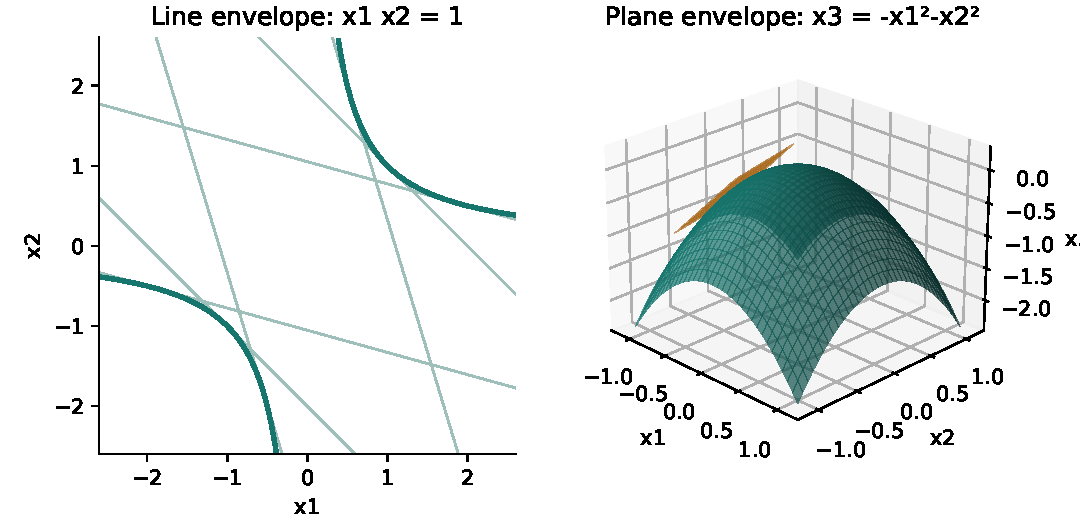
\includegraphics[width=\linewidth]{output/figures/ch03-envelopes.pdf}
\end{center}
\noindent\textit{Editorial figure for Problem 2.}
A hyperbola is tangent to a family of lines; a negative paraboloid
is tangent to the associated family of planes. Elimination and
parameter-domain restrictions are worked out in the exercise solution.

% Evans second edition, section 3.2.
% English source: printed p. 94; PDF page 111 (1-based).
% Chinese section starts: checked against the chapter-opening list, PDF p. 79.
% Status: editorial study draft with detailed proofs and mathematical notes; no independent review.
\Needspace{65mm}
\section{Characteristics}
\label{sec:3-2}

\subsection{Deriving the full characteristic system (Evans \S3.2.1)}
Suppose first that a $C^2$ solution exists. Along a curve $X(s)$ set
$Z(s)=u(X(s))$ and $P(s)=Du(X(s))$.
Then
\[
 \dot P_i=\sum_j u_{x_ix_j}(X)\dot X_j.
\]
Differentiate the PDE itself in $x_i$:
\[
 \sum_j F_{p_j}u_{x_jx_i}+F_z u_{x_i}+F_{x_i}=0.
\]
Choosing $\dot X_j=F_{p_j}$ makes the unknown Hessian sum match
the first expression. Hence
\[
 \boxed{\begin{aligned}
 \dot X&=F_p(P,Z,X),\\
 \dot P&=-F_x(P,Z,X)-F_z(P,Z,X)P,\\
 \dot Z&=P\cdot F_p(P,Z,X).
 \end{aligned}}
 \tag{CH}
\]
All partial derivatives of $F$ here hold its other arguments fixed.
The third equation is the chain rule for $u(X(s))$.
\Needspace{45mm}
\PDEAnnotation{选择路径是为了消去 Hessian}{任意路径的梯度变化含 $D^2u$，并不封闭。取速度 $F_p$ 后，恰好能用微分后的 PDE 替换这组二阶导数，得到只含 $X,P,Z$ 的 ODE。}

\paragraph{An invariant of the system.}
Even before knowing $P=Du$, solutions of (CH) satisfy
\[
 \frac d{ds}F(P,Z,X)
 =F_p\cdot(-F_x-F_zP)+F_z(P\cdot F_p)+F_x\cdot F_p=0.
\]
Initial data with $F(P(0),Z(0),X(0))=0$ therefore remain on the
PDE constraint surface. This invariant alone does not yet prove
that the transported vector $P$ is the gradient of a single-valued function.

\subsection{Reduced systems and explicit examples (Evans \S3.2.2)}
For $b(x)\cdot Du+c(x)u=f(x)$, only
\[
 \dot X=b(X),\qquad \dot Z=f(X)-c(X)Z
\]
are needed to compute values.
If $b=b(x,u)$, the value equation remains
$\dot Z=-c(X,Z)$ for $b(x,u)\cdot Du+c(x,u)=0$;
the path now depends on the unknown value.

\paragraph{Rotation.}
For $x_1u_{x_2}-x_2u_{x_1}=u$ in the first quadrant with
$u(r,0)=g(r)$,
\[
 X(s)=(r\cos s,r\sin s),\qquad Z(s)=e^s g(r).
\]
Thus
$u(x_1,x_2)=e^{\arctan(x_2/x_1)}g(\sqrt{x_1^2+x_2^2})$.
This is also immediate from $u_\theta=u$ in polar coordinates.

\paragraph{Value blow-up without crossing.}
For $u_{x_1}+u_{x_2}=u^2$, $u(x_1,0)=g(x_1)$,
\[
 X(s)=(r+s,s),\qquad Z(s)=\frac{g(r)}{1-sg(r)},
\]
so
\[
 u(x_1,x_2)=\frac{g(x_1-x_2)}
                      {1-x_2g(x_1-x_2)}
\]
on the connected region reached before a denominator vanishes.
If $g(r)>0$, the characteristic value blows up at $s=1/g(r)$.
Continuing the rational expression beyond its pole is not continuing
a finite classical solution through the blow-up time.
\Needspace{45mm}
\PDEAnnotation{两种失效机制}{半线性例子可在路径不相交时因 $Z$ 爆破失效；守恒律常见的是值仍有界、空间梯度先爆破。只检查特征线位置还不够。}

\paragraph{A fully nonlinear example.}
For $u_{x_1}u_{x_2}=u$, $u(0,r)=r^2$, compatibility gives
$P_2(0)=2r$ and $P_1(0)=r/2$ when $r\ne0$.
The system is $\dot P_i=P_i$, $\dot X_1=P_2$,
$\dot X_2=P_1$, $\dot Z=2P_1P_2$.
It integrates to
\[
 X_1=2r(e^s-1),\quad X_2=\tfrac r2(e^s+1),\quad Z=r^2e^{2s}.
\]
Since $4X_2-X_1=4r$ and $4X_2+X_1=4re^s$,
\[
 u(x_1,x_2)=\frac{(x_1+4x_2)^2}{16}.
\]
Direct differentiation verifies the PDE and boundary data everywhere.
The characteristic construction just given is locally invertible only
where $r\ne0$; the polynomial formula extends across the excluded locus.
An explicit extension does not mean the local existence theorem was
applicable at the characteristic boundary point $r=0$.

\subsection{Admissible and noncharacteristic data (Evans \S3.2.3)}
Flatten the initial hypersurface to $x_n=0$ and write its coordinates
as $y\in\R^{n-1}$. Prescribing $u(y,0)=g(y)$ fixes
\[
 Z(0)=g(y),\quad P_i(0)=g_{y_i}(y)\ (i<n),\quad
 F(P(0),g(y),(y,0))=0.
 \tag{IC}
\]
Only the normal derivative $P_n(0)$ remains to be found.
At an admissible root $p^0$, the sufficient condition
$F_{p_n}(p^0,g(y_0),(y_0,0))\ne0$
lets the implicit function theorem solve for a smooth branch $q_n(y)$.
Different roots may produce different local solutions; uniqueness is
relative to the chosen admissible branch.
\Needspace{45mm}
\PDEAnnotation{边界值没有给出完整梯度}{沿边界求导只能得到切向分量，法向分量要由 PDE 求出。代数方程可能无根或多根；非特征条件保证的是已选根附近的局部唯一分支。}

For a curved surface, choose a smooth extension of $g$ and write
$p=D_{\tan}g+\lambda\nu$, where $\nu$ is its unit normal.
Differentiating the scalar constraint in $\lambda$ gives
\[
 \frac d{d\lambda}F(D_{\tan}g+\lambda\nu,g,x)
       =F_p\cdot\nu.
\]
Thus the invariant geometric noncharacteristic condition is
$F_p\cdot\nu\ne0$: the characteristic velocity crosses the surface.
Changing the normal's orientation changes the sign, not this condition.

For example $u_{x_2}=0$ with data on $x_2=0$ is noncharacteristic.
The equation $u_{x_1}=0$ on the same boundary is characteristic:
nonconstant data in $x_1$ are incompatible, while constant data leave
the $x_2$ dependence undetermined. Failure of the hypothesis can mean
either nonexistence or nonuniqueness.


\PDEBodyDiagram{3.1}{Noncharacteristic data permit local reconstruction.}
{The projected characteristic direction is $F_p$. Transversality makes the initial-surface parameters together with the flow parameter independent local coordinates. A tangent direction makes this coordinate construction singular; it does not by itself prove that no solution can exist.}
{ch03-transverse}

\subsection{Reconstructing a local solution (Evans \S3.2.4, Theorem 2)}
\Needspace{45mm}
\PDEAnnotation{非特征条件是局部条件}{$F_p\cdot\nu\ne0$ 让特征穿过初始曲面，从而给出局部坐标。它不保证以后投影仍可逆；法向速度的正负另用于区分流入、流出方向。}
\begin{theorem}\label{thm:3-local}
For smooth $F,g$ and a chosen admissible noncharacteristic triple,
(CH) with data (IC) reconstructs a smooth local solution.
The construction is unique locally among smooth solutions sharing
that branch of boundary gradient.
\end{theorem}
\begin{expandedproof}[including the gradient compatibility step]
\paragraph{1. Solve the ODE with boundary parameters.}
Use the boundary-parameterized solution
\[
 (X,P,Z)(y,0)=((y,0),q(y),g(y)).
\]
Local ODE theory with smooth dependence supplies a common parameter neighborhood.
At $s=0$, the columns $X_{y_i}$ are $e_i$, $i<n$, and
$X_s=F_p$. Hence
\[
 \det D_{(y,s)}X(y_0,0)=F_{p_n}(p^0,z^0,x^0)\ne0.
\]
The inverse function theorem gives local coordinates
$(y,s)=(y(x),s(x))$. Define $u(x)=Z(y(x),s(x))$.

\paragraph{2. Preserve the algebraic PDE constraint.}
The invariant above and initial compatibility give
$F(P(y,s),Z(y,s),X(y,s))=0$.
We still have to prove $P(y,s)=Du(X(y,s))$.

\paragraph{3. Propagate the contact identities.}
The $s$ identity $Z_s=P\cdot X_s$ is in (CH).
For every boundary parameter set
$R_i=Z_{y_i}-P\cdot X_{y_i}$.
Initially $R_i=0$, by the tangential compatibility in (IC).
Differentiate:
\[
 \begin{split}
 (R_i)_s
 &=P_{y_i}\cdot X_s-P_s\cdot X_{y_i}\\
 &=F_p\cdot P_{y_i}+F_x\cdot X_{y_i}
                         +F_zP\cdot X_{y_i}.
 \end{split}
\]
Differentiating the preserved identity $F(P,Z,X)=0$ in $y_i$ yields
$F_p\cdot P_{y_i}+F_x\cdot X_{y_i}=-F_zZ_{y_i}$.
Therefore $(R_i)_s=-F_zR_i$ with zero initial value.
Uniqueness for this scalar linear ODE gives $R_i=0$.

\paragraph{4. Return to physical coordinates.}
Together the identities say $dZ=P\cdot dX$ for all parameter
differentials. Since $D_{(y,s)}X$ is invertible, every physical
differential occurs, so $Du=P$.
The preserved constraint now becomes $F(Du,u,x)=0$.
At $s=0$ we recover $u=g$. Any other smooth solution with the same
boundary gradient branch generates the same characteristic ODE data,
so ODE uniqueness and coordinate invertibility identify the solutions.
\end{expandedproof}
\Needspace{45mm}
\PDEAnnotation{不能提前把 $P$ 叫作梯度}{从 ODE 构造出来的 $P$ 起初只是向量场。必须证明 $dZ=P\cdot dX$，再利用坐标可逆性，才能认定 $P=Du$；否则只保留 $F(P,Z,X)=0$ 还没有解出 PDE。}

\subsection{Evolution equations and breakdown (Evans \S3.2.5)}
For $u_t+\mathbf f'(u)\cdot D_xu=0$ with initial data $g$,
\[
 X(a,t)=a+t\mathbf f'(g(a)),\qquad u(X(a,t),t)=g(a).
\]
Eliminating $a$ gives $u=g(x-t\mathbf f'(u))$ while the map is invertible.
Its Jacobian is $I+t\,\mathbf f''(g(a))\otimes Dg(a)$.
The rank-one determinant identity yields
\[
 \det D_aX=1+t\,Dg(a)\cdot\mathbf f''(g(a)).
\]
In one dimension,
\[
 u_x(X(a,t),t)=\frac{g'(a)}
                    {1+t f''(g(a))g'(a)}.
\]
If the denominator first vanishes with $g'(a)<0$ and $f''>0$,
gradients blow up although $u=g(a)$ remains finite.
For Burgers flux $f(u)=u^2/2$ and bounded $C^1$ data with
$m=\inf g'<0$, the first loss of a uniform positive Jacobian is at
$T_*=-1/m$. If the infimum is attained, that characteristic gives
an actual zero Jacobian at $T_*$.
\Needspace{45mm}
\PDEAnnotation{相空间不交不保证投影不交}{扩展状态 $(X,P,Z)$ 的 ODE 可保持唯一性，但只看 $X$ 时不同状态可落在同一位置。物理空间的逆映射失效，正是特征构造中光滑解失效的关键。}

For $u_t+H(D_xu,x)=0$, the full system becomes Hamilton's equations
and an action equation:
\[
 \dot X=H_p(P,X),\qquad
 \dot P=-H_x(P,X),\qquad
 \dot Z=P\cdot H_p-H.
\]
When $H=H(p)$, $P=Dg(a)$ stays constant and
\[
 X=a+tDH(Dg(a)),\qquad
 Z=g(a)+t[Dg(a)\cdot DH(Dg(a))-H(Dg(a))].
\]
This formula is local until the projection ceases to be invertible.
The next section gives a variational continuation with a selection rule.

% Evans second edition, section 3.3.
% English source: printed p. 110; PDF page 127 (1-based).
% Chinese section starts: checked against the chapter-opening list, PDF p. 79.
% Status: editorial study draft with detailed proofs and mathematical notes; no independent review.
\Needspace{65mm}
\section{Introduction to Hamilton--Jacobi Equations}
\label{sec:3-3}

\subsection{Variations and Hamilton's ODE (Evans \S3.3.1)}
For a path $X:[0,t]\to\R^n$ with fixed endpoints consider
\[
 \mathcal A[X]=\int_0^t L(\dot X(s),X(s))\,ds.
\]
Suppose a smooth minimizer exists. For every smooth variation $V$
vanishing at both endpoints, differentiate the action at $X+\varepsilon V$:
\[
 0=\int_0^t[L_v(\dot X,X)\cdot\dot V+L_x(\dot X,X)\cdot V]\,ds.
\]
Integration by parts, with the endpoint terms zero, gives
$\frac d{ds}L_v(\dot X,X)=L_x(\dot X,X)$ by the fundamental lemma
of the calculus of variations. These are the Euler--Lagrange equations.
They are necessary conditions; their derivation does not prove a
minimizer exists or that every stationary path minimizes.

Assume now the velocity--momentum relation $P=L_v(v,x)$ can be inverted,
and define
$H(P,x)=P\cdot v(P,x)-L(v(P,x),x)$.
In differentiating this identity the terms containing derivatives of
$v$ cancel because $P=L_v$. Thus $H_p=v$ and $H_x=-L_x$.
The Euler--Lagrange equations become
\[
 \dot X=H_p(P,X),\qquad \dot P=-H_x(P,X).
\]
For $L(v,x)=|v|^2/2-V(x)$ this gives $P=v$,
$H=|P|^2/2+V(x)$ and $\ddot X=-DV(X)$.
For an autonomous Hamiltonian,
$\frac d{ds}H=H_p\cdot(-H_x)+H_x\cdot H_p=0$.
\Needspace{45mm}
\PDEAnnotation{两个来源得到同一组 ODE}{变分法从作用量的驻值推出 Hamilton 方程；特征线法从 Hamilton--Jacobi PDE 推出同一方程。前者给出力学意义，后者解释它如何搬运函数与梯度。}

\subsection{Convex duality and Hopf--Lax (Evans \S3.3.2)}
\label{sec:3-hopflax}
A function $A$ is superlinear if $A(v)/|v|\to+\infty$ as $|v|\to\infty$.
For a finite convex function define
\[
 A^*(p)=\sup_v\{p\cdot v-A(v)\}.
\]
Superlinearity of $A$ makes the objective tend to $-\infty$,
so the maximum is attained and $A^*$ is finite.
It is convex as a supremum of affine functions.
For every $R>0$,
\[
 A^*(p)\geq R|p|-\max_{|v|=R}A(v);
\]
hence $A^*$ is also superlinear when $A$ is finite everywhere.

\begin{theorem}[Convex duality; source Theorem 3]
For finite convex superlinear $A$, $A^{**}=A$ and
\[
 A(v)+A^*(p)\geq p\cdot v.
\]
Equality holds precisely when $p$ is a supporting slope of $A$ at $v$.
For differentiable $A$, this means $p=DA(v)$.
\end{theorem}
\begin{expandedproof}
The inequality is the definition of the supremum.
A supporting slope satisfies
$A(w)\geq A(v)+p\cdot(w-v)$ for every $w$.
Rearranging shows the supremum defining $A^*(p)$ is attained at $v$,
giving equality. Conversely equality rearranges to that support inequality.
Always $A^{**}(v)\leq A(v)$. Choose a supporting slope at $v$;
then the equality just established gives the reverse inequality.
Existence of supporting hyperplanes for finite convex functions is
the invoked convex-analysis prerequisite.
For a differentiable convex function the tangent-plane inequality
provides this slope directly as $DA(v)$.
\end{expandedproof}
The supporting-plane argument for $A^{**}=A$ also holds for every
finite convex $A$ without superlinearity; in that case $A^*$ may take
the value $+\infty$. Subdifferentials of such extended-valued functions
are taken only at points where the function is finite.
\Needspace{45mm}
\PDEAnnotation{对偶变换中的极大值}{求 $v\cdot p-H(p)$ 的驻点只是候选；凸性让该目标关于 $p$ 凹，超线性增长使它在无穷远趋负无穷，才保证极大值确实取得。}

\PDEBodyDiagram{3.2}{Legendre duality is a supporting-line construction.}
{For $H(p)=p^2/2$ and $v=1$, maximizing $vp-H(p)$ finds the tangent point $p=1$. The tangent's intercept is $-L(1)=-1/2$. Convexity makes the whole graph lie above this line, which is exactly the Fenchel inequality.}
{ch03-legendre-support}

For the rest of this subsection assume $H$ is finite, convex, smooth
and superlinear on $\R^n$, set $L=H^*$, and let $g$ be globally
Lipschitz with constant $K$. Then $L$ is finite, convex and superlinear,
and $H=L^*$.

\Needspace{45mm}
\PDEAnnotation{超线性排除逃向远方的起点}{$g$ 的下降至多是线性的，而 $tL((x-y)/t)$ 在位移很大时增长更快。这不仅给出最小值存在，还把最优起点限制在 $|x-y|\leq Rt$ 内。}
\paragraph{Why a straight path gives the formula (source Theorem 4).}
Since $L$ no longer depends on position, Jensen's inequality gives
for any absolutely continuous path with $X(0)=y$, $X(t)=x$,
\[
 \int_0^tL(\dot X(s))\,ds
 \geq tL\left(\frac1t\int_0^t\dot X(s)\,ds\right)
 =tL((x-y)/t).
\]
The straight path $X(s)=y+s(x-y)/t$ attains equality.
Minimizing over its starting point gives
\[
 \boxed{u(x,t)=\min_{y\in\R^n}
             \{tL((x-y)/t)+g(y)\}.}
 \tag{HL}
\]
The minimum exists: with $v=(x-y)/t$, its objective is at least
$g(x)+t[L(v)-K|v|]$, coercive in $v$.
Comparing with $y=x$ also proves that every minimizer satisfies
$L(v)-K|v|\leq L(0)$, hence $|v|\leq R_K$ for a fixed finite $R_K$.
This is the first finite-range localization of the minimization.
\Needspace{45mm}
\PDEAnnotation{直线最优依赖哪些条件}{这里用到 $L$ 的凸性和无位置依赖。若 $L=L(v,x)$，不同路径经过不同势场，不能只用端点位移除以时间就替代整条作用量。}


\PDEMarginDiagram{3.M}{把路径在中途切开}
{中间点 $z$ 也要优化。两段代价相加后再取下确界，才得到动态规划恒等式。}
{ch03-path-split-margin}

\begin{lemma}[Dynamic programming; source Lemma 1]\label{lem:3-dpp}
For $0<s<t$,
\[
 u(x,t)=\min_z\{(t-s)L((x-z)/(t-s))+u(z,s)\}.
 \tag{DP}
\]
\end{lemma}
\begin{expandedproof}
For any $z$ and a minimizing starting point $y$ for $u(z,s)$,
convexity applied to
$(x-y)/t=[(t-s)/t](x-z)/(t-s)+(s/t)(z-y)/s$
gives
$u(x,t)\leq(t-s)L((x-z)/(t-s))+u(z,s)$.
This proves one inequality for the infimum over $z$.
Conversely take a minimizer $y$ in (HL) and choose
$z=y+(s/t)(x-y)$. Both subinterval velocities then equal $(x-y)/t$.
Use this same $y$ as a competitor for $u(z,s)$ to obtain the opposite
inequality. Coercivity ensures the intermediate minimum exists.
\end{expandedproof}

\begin{lemma}[Lipschitz bounds and initial values; source Lemma 2]
The function in (HL) is globally Lipschitz in $(x,t)$ for $t\geq0$,
when defined by $u(x,0)=g(x)$.
\end{lemma}
\begin{expandedproof}
If $y$ minimizes at $x$, use $y+h$ as competitor at $x+h$.
The velocity is unchanged, so $u(x+h,t)-u(x,t)\leq K|h|$.
Exchange $x,x+h$ for the reverse inequality.

For time zero, the competitor $y=x$ gives
$u(x,t)\leq g(x)+tL(0)$, while duality gives
\[
 u(x,t)\geq g(x)+t\inf_v[L(v)-K|v|]
 =g(x)-t\max_{|p|\leq K}H(p).
\]
Thus $|u(x,t)-g(x)|\leq Ct$, uniformly in $x$, with
\[
 C=\max\{|L(0)|,\max_{|p|\leq K}|H(p)|\}.
\]
Apply the same argument to (DP), using the spatial Lipschitz bound
for $u(\cdot,s)$, to get $|u(x,t)-u(x,s)|\leq C|t-s|$.
\end{expandedproof}


\PDEBodyDiagram{3.3}{Equal minimizing costs can produce a corner in the value.}
{With $H(p)=p^2/2$, $t=1$ and $g(y)=\max(-|y|,-2)$, the Hopf--Lax cost at $x=0$ has two minimizers $y=\pm1$. Their candidate endpoint slopes $(x-y)/t$ differ. Indeed near $x=0$ the value is $u(x,1)=-1/2-|x|$, so it is not differentiable there.}
{ch03-hopflax-tie}

\begin{theorem}[PDE at differentiability points; source Theorems 5--6]
The Hopf--Lax function satisfies $u_t+H(Du)=0$ at every point where
it is differentiable, hence almost everywhere by Rademacher's theorem.
\end{theorem}
\begin{expandedproof}
At a differentiability point $(x,t)$, (DP) with the competitor $x$
over a short forward time gives
$u(x+hv,t+h)\leq hL(v)+u(x,t)$ for every fixed $v$.
Divide by $h>0$ and pass to zero:
$u_t+v\cdot Du\leq L(v)$. Supremizing in $v$ yields
$u_t+H(Du)\leq0$.

For the other sign choose a minimizing $y$ in (HL) at $(x,t)$ and
put $v_*=(x-y)/t$.
At time $t-h$, $z=x-hv_*$ lies on the straight minimizing path.
Using $y$ as competitor there yields
$u(x,t)-u(z,t-h)\geq hL(v_*)$.
Differentiability gives $u_t+v_*\cdot Du\geq L(v_*)$.
Since $H(Du)\geq v_*\cdot Du-L(v_*)$, the reverse sign follows.
Neither argument differentiates a potentially nonsmooth minimizing
point $y(x,t)$.
\end{expandedproof}
\Needspace{45mm}
\PDEAnnotation{最小值不一定可微}{多个最优起点可能同时出现，不能直接对 $y(x,t)$ 求导。动态规划用固定竞争者给一侧不等式，再沿一条最优路径给另一侧，避开了这个问题。}

For $H(p)=|p|^2/2$, $L(v)=|v|^2/2$ and
$u(x,t)=\min_y\{|x-y|^2/(2t)+g(y)\}$.
At a smooth minimizing branch,
$(x-y)/t=Dg(y)$, so $x=y+tDg(y)$ and $Du=Dg(y)$,
recovering the local characteristic formulas.
When branches compete, the minimum remains meaningful even though
their smooth projection has broken down.

\input{chapters/03-nonlinear-first-order-pde/03a-semiconcavity-uniqueness}

% Evans second edition, section 3.4.
% English source: printed p. 130; PDF page 147 (1-based).
% Chinese section starts: checked against the chapter-opening list, PDF p. 79.
% Status: editorial study draft with detailed proofs and mathematical notes; no independent review.
\Needspace{65mm}
\section{Introduction to Conservation Laws}
\label{sec:3-4}

\subsection{Shocks and entropy (Evans \S3.4.1)}
We now work in one space dimension:
\[
 u_t+f(u)_x=0,\qquad u(x,0)=g(x).
\]
The conservative form must be retained after smoothness breaks down.
An integral solution is a locally bounded function satisfying
\[
 \int_0^\infty\!\!\int_{\R}[u\phi_t+f(u)\phi_x]\,dx\,dt
       +\int_{\R}g(x)\phi(x,0)\,dx=0
 \tag{CL}
\]
for every smooth compactly supported test function on $\R\times[0,\infty)$.
For smooth $u$, integration by parts proves equivalence with the PDE.
For discontinuous $u$, the expression $f'(u)u_x$ is not an ordinary
product of functions and cannot replace (CL) without additional theory.
\Needspace{45mm}
\PDEAnnotation{先守恒后求导}{光滑时 $f(u)_x=f'(u)u_x$；跳跃时 $u_x$ 含集中测度。守恒形式能直接对 $f(u)$ 作分布求导，避免给不连续函数与 Dirac 的乘积随意赋值。}

\begin{theorem}[Rankine--Hugoniot]\label{thm:3-rh}
Across a smooth shock curve $x=\gamma(t)$ with traces $u_l,u_r$,
an otherwise smooth integral solution must satisfy
\[
 \gamma'(t)(u_r-u_l)=f(u_r)-f(u_l).
 \tag{RH}
\]
For unequal states, the speed is the secant slope of $f$.
\end{theorem}
\begin{expandedproof}
Write locally $u=u_l+(u_r-u_l)\mathbf1_{\{x>\gamma(t)\}}$,
with the smooth extensions on each side understood.
The singular part of $u_t$ is $-\gamma'[u]\delta_{x=\gamma(t)}$;
that of $f(u)_x$ is $[f]\delta_{x=\gamma(t)}$.
Here $[u]=u_r-u_l$ and $[f]=f(u_r)-f(u_l)$.
The regular parts vanish by the PDE on each side.
The remaining distribution is zero precisely when (RH) holds.
Equivalently, integrate each smooth side of (CL) and add their
oppositely oriented interface fluxes.
\end{expandedproof}

For strictly convex $f$, an admissible shock has $u_l>u_r$.
Its speed satisfies
$f'(u_r)<\gamma'<f'(u_l)$, since secant slopes lie strictly between
endpoint tangent slopes.
Characteristics enter the shock from both sides.
An upward jump also satisfies (RH) with its secant speed, but would
send characteristics outward and is rejected by entropy.


\PDEBodyDiagram{3.4}{Shock speed is a secant slope.}
{For $f(u)=u^2/2$, the secant between $u_R=0.2$ and $u_L=1.4$ has slope $\sigma=0.8$. The tangent slopes satisfy $0.2<0.8<1.4$, so characteristics from both sides enter the shock. Reversing the spatial states keeps the secant slope but violates the compression direction.}
{ch03-flux-chord}

\paragraph{Why weak conservation alone is not unique.}
For Burgers flux $f(u)=u^2/2$ and data $g=0$ on $x<0$, $g=1$ on $x>0$,
both the upward step moving at speed $1/2$ and
\[
 u(x,t)=\begin{cases}
 0,&x\leq0,\\ x/t,&0<x<t,\\1,&x\geq t
 \end{cases}
\]
satisfy (CL). In the fan the PDE is
$-x/t^2+(x/t)(1/t)=0$, and both interfaces are continuous.
Each candidate attains the same initial data in local $L^1$.
Only the fan satisfies the one-sided bound derived below.
\Needspace{45mm}
\PDEAnnotation{跳跃条件不负责筛选方向}{Rankine--Hugoniot 只保证接口两侧通量守恒，上跳和下跳都可能满足。熵条件额外保留压缩型跳跃，排除向外散开的非物理解。}

\paragraph{Convex entropy pairs: an editorial explanation.}
For smooth convex $\eta$, define $q$ by $q'=\eta'f'$.
A smooth solution satisfies $\eta(u)_t+q(u)_x=0$.
For the viscous equation $u_t+f(u)_x=\varepsilon u_{xx}$,
\[
 \eta(u)_t+q(u)_x
 =\varepsilon\partial_{xx}\eta(u)
       -\varepsilon\eta''(u)|u_x|^2
 \leq\varepsilon\partial_{xx}\eta(u).
\]
If bounded viscous solutions converge strongly locally, their limit
therefore satisfies the distributional entropy inequality.
This is a conditional explanation of the selection rule, not a proof
of viscous existence or convergence.

For a downward shock $l=u_l>u_r=r$ with secant speed $s$, let
$C(v)=f(v)-f(r)-s(v-r)\leq0$ on $[r,l]$.
The singular entropy coefficient is
\[
 [q]-s[\eta]=-\int_r^l\eta'(v)C'(v)\,dv
            =\int_r^l\eta''(v)C(v)\,dv\leq0.
\]
Thus the convex entropy inequality selects the same direction.
For general nonsmooth solutions this chapter uses the source's
one-sided derivative condition as its explicit uniqueness class.

\subsection{The Lax--Oleinik construction (Evans \S3.4.2)}
\label{sec:3-laxoleinik}
Assume $f$ smooth and $f''\geq\theta>0$ on $\R$, and $g\in L^\infty$.
An additive constant in $f$ does not affect the PDE; take $f(0)=0$.
Let
\[
 P(x)=\int_0^xg(y)\,dy,\qquad
 L=f^*,\qquad G=(f')^{-1}=L'.
\]
The potential
\[
 W(x,t)=\min_y\{tL((x-y)/t)+P(y)\}
 \tag{LOP}
\]
is a Hopf--Lax solution of $W_t+f(W_x)=0$.
The candidate conservation-law solution is $u=W_x$ a.e.
\Needspace{45mm}
\PDEAnnotation{HJ 解是守恒律解的原函数}{$W_t+f(W_x)=0$ 对空间作分布求导，就得到 $u_t+f(u)_x=0$。给初始原函数 $P$ 加常数只会给 $W$ 加同一常数，不改变 $u$ 或最优起点。}
Since $f'$ is strictly increasing and onto, $G$ exists and is
$1/\theta$-Lipschitz. Differentiating the convex dual at its unique
maximizer gives $L'=G$ and $L''=1/f''(G)>0$.

\begin{theorem}[Source Theorem 1]\label{thm:3-lo}
For each $t>0$, minimizing starting points in (LOP) are ordered with $x$.
The minimizer is unique except at at most countably many $x$.
At differentiability points of $W$,
\[
 \boxed{u(x,t)=G((x-y(x,t))/t).}
 \tag{LO}
\]
\end{theorem}
\begin{expandedproof}
\paragraph{1. Ordering and countability.}
Put $c(x,y)=tL((x-y)/t)$.
Its mixed derivative is $c_{xy}=-L''((x-y)/t)/t<0$.
If $x_1<x_2$ and proposed minimizers had $y_1>y_2$,
integration of this mixed derivative on the rectangle gives
\[
 c(x_1,y_2)+c(x_2,y_1)<c(x_1,y_1)+c(x_2,y_2).
\]
Adding $P(y_1)+P(y_2)$ contradicts the sum of the two minimizing
inequalities. Hence every minimizer at $x_1$ is at most every minimizer
at $x_2$.
The minimum sets are nonempty compact sets by coercivity.
If a set has two distinct endpoints $y_-<y_+$, its interval
$(y_-,y_+)$ is disjoint from the corresponding intervals for other $x$.
Assigning a rational point to each nonempty interval proves there are
at most countably many such $x$.

\Needspace{45mm}
\PDEAnnotation{可数例外指固定的时间切片}{每个多重最优点对应一个互不相交的起点开区间，再各选一个有理数，才得到可数性。这不表示整个时空只存在可数个激波点，也不等于全局光滑。}
\paragraph{2. Differentiate the value without differentiating the optimizer.}
For a fixed minimizing $y$, use that same point as a competitor at
$x+h$. Then
$W(x+h,t)-W(x,t)\leq c(x+h,y)-c(x,y)$.
For positive and negative $h$, differentiability of $W$ gives
$W_x=L'((x-y)/t)=G((x-y)/t)$.
This works even if $P$ is not differentiable at the minimizing $y$.
Strict monotonicity of $G$ also forces uniqueness of $y$ at such a point.
\end{expandedproof}
\Needspace{45mm}
\PDEAnnotation{最优起点的跳跃产生激波}{$y(x,t)$ 保持单调，但可发生跳跃。跨过竞争分支时，$(x-y)/t$ 随之下降，因此 $u=G((x-y)/t)$ 出现向下跳跃；这把变分选择和熵方向联系起来。}

\begin{theorem}[Integral solution and initial trace; source Theorem 2]
The construction gives a bounded integral solution of (CL).
It satisfies $u(\cdot,t)\to g$ in $L^1_{\mathrm{loc}}$ as $t\downarrow0$.
\end{theorem}
\begin{expandedproof}
First $W$ is spatially Lipschitz with constant $\|g\|_\infty$, hence
$|u|\leq\|g\|_\infty$ a.e.
The a.e. HJ equation $W_t+f(W_x)=0$ is an equality of locally integrable
functions. Multiply it by $\phi_x$.
Integration by parts first in time and then in space gives
\[
 \iint W_t\phi_x
 =-\iint W\phi_{xt}-\int P\phi_x(\cdot,0)
 =\iint W_x\phi_t+\int g\phi(\cdot,0).
\]
All supports are compact and $W$ is Lipschitz; thus these are valid
weak integration identities. Substituting $u=W_x$ proves (CL).

To strengthen initial recovery, fix a Lebesgue point $x$ of $g$,
with value $g_0$. Then
$P(x+h)=P(x)+g_0h+o(|h|)$.
The coercive minimizer bound gives $|x-y|/t\leq R$ uniformly.
Writing $y=x-tv$, the minimizing objective becomes
\[
 P(x)+t[L(v)-g_0v]+o(t)
\]
uniformly for $|v|\leq R$.
The strictly convex function $L(v)-g_0v$ has unique minimizer
$v_*=f'(g_0)$. Compactness implies every minimizing velocity tends
to $v_*$: otherwise a convergent subsequence away from $v_*$ would
minimize the limiting strictly convex objective.
Formula (LO) therefore gives $u(x,t)\to G(v_*)=g_0$.
The uniform $L^\infty$ bound and dominated convergence on compact
intervals give the asserted local $L^1$ convergence.
\end{expandedproof}

\input{chapters/03-nonlinear-first-order-pde/04a-entropy-uniqueness}

\subsection{Riemann's problem (Evans \S3.4.4, Theorem 4)}
For $g=u_l$ on $x<0$ and $g=u_r$ on $x>0$, the entropy solution for
a strictly convex flux is as follows.
If $u_l>u_r$, it is a shock with speed
$s=[f(u_l)-f(u_r)]/(u_l-u_r)$.
If $u_l<u_r$, it is the rarefaction
\[
 u(x,t)=\begin{cases}
 u_l,&x/t\leq f'(u_l),\\
 G(x/t),&f'(u_l)<x/t<f'(u_r),\\
 u_r,&x/t\geq f'(u_r).
 \end{cases}
 \tag{RF}
\]
Equal states give a constant solution.
\begin{expandedproof}
The shock satisfies the PDE off its interface, (RH) on it, and the
downward entropy direction.
In the fan, $u_t=-(x/t^2)G'(x/t)$ and
$f'(u)u_x=(x/t)G'(x/t)/t$, which cancel.
The fan joins continuously to both constant states and
$u_x=G'(x/t)/t\leq1/(\theta t)$.
Both candidates are integral solutions and approach their Riemann data
locally in $L^1$; the transition region has width $O(t)$.
The entropy uniqueness theorem just proved identifies them as the
selected solutions.
\end{expandedproof}
\begin{center}
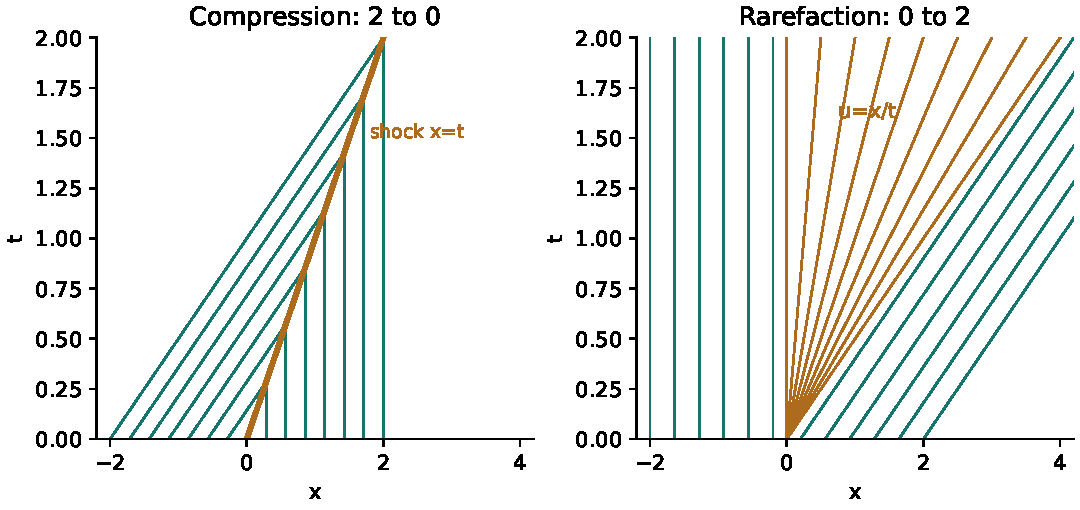
\includegraphics[width=\linewidth]{output/figures/ch03-riemann-characteristics.pdf}
\end{center}
\noindent\textit{Editorial figure.} For Burgers flow, a downward step
compresses characteristics into a shock; an upward step opens a
rarefaction fan. Both geometries use the same flux, but different data.

\input{chapters/03-nonlinear-first-order-pde/04b-long-time-behavior}

% Evans second edition, section 3.5.
% English source: printed p. 154; PDF page 171 (1-based).
% Chinese section starts: checked against the chapter-opening list, PDF p. 79.
% Status: editorial study draft with detailed proofs and mathematical notes; no independent review.
\Needspace{65mm}
\section{Problems}
\label{sec:3-5}

\noindent\textit{Source: Evans \S3.5, Problems 1--20, printed pp.~154--158
(PDF pp.~171--175).} Statements below are concisely restated.
All solutions are editorial, with smoothness assumed where required;
extensions beyond the smooth class are identified explicitly.

\subsection{Problems 1--8: envelopes and characteristics}
\Needspace{30mm}
\paragraph{1. A complete Hamilton--Jacobi integral.}
\begin{proof}[Solution]
For $U=a\cdot x-tH(a)+b$, $D_xU=a$ and $U_t=-H(a)$, proving the PDE.
There are $n+1$ parameters for $n+1$ independent variables.
The derivatives with respect to $a_i$ independently vary $D_xU$;
the derivative with respect to $b$ changes the value by one without
changing any gradient component.
These $n+1$ jet variations are linearly independent, proving completeness.
\end{proof}

\Needspace{30mm}
\paragraph{2. Envelopes of lines and planes.}
\begin{proof}[Solution]
For $G=x_1+a^2x_2-2a$, the stationary condition is $G_a=2ax_2-2=0$.
Thus $a\ne0$, $x_2=1/a$, and $G=0$ then gives $x_1=a$.
The envelope is $x_1x_2=1$, with both branches represented.
The line with $a=0$ has no finite stationary contact.
For $G=2a_1x_1+2a_2x_2-x_3+a_1^2+a_2^2$,
stationarity yields $a_i=-x_i$ and elimination gives
$x_3=-x_1^2-x_2^2$.
The derivatives of this paraboloid equal the slopes $2a_i$ of the
selected plane, directly verifying tangency. The figure in \S3.1
shows both constructions.
\end{proof}

\Needspace{30mm}
\paragraph{3. Eliminate parameters to obtain a PDE.}
\begin{proof}[Solution]
(a) For $\sum_i a_ix_i^2+u^3=0$, implicit differentiation gives
$2a_ix_i+3u^2u_{x_i}=0$.
Multiply by $x_i$, sum, and eliminate $\sum_i a_ix_i^2=-u^3$:
\[
 u^2(3x\cdot Du-2u)=0.
\]
On a nonzero branch this is $3x\cdot Du=2u$.
For a $C^1$ graph it extends to the zero set by continuity from
nonzero points, while on the interior of $\{u=0\}$ the gradient is zero.
This avoids division by a possibly zero coordinate $x_i$.

(b) A unit sphere centered at $(a,0)$ has
$|x-a|^2+u^2=1$. Differentiation yields $x-a=-uDu$.
Substitution eliminates $a$ and gives $u^2(1+|Du|^2)=1$,
on regions where the sphere is a differentiable graph.
\end{proof}
\Needspace{45mm}
\PDEAnnotation{参数消元要记录分支}{除以 $u$、$x_i$ 或某个行列式前，先说明它不为零。得到的简化 PDE 可能丢掉零解或特殊分支；保留未约去的形式有助于检查。}

\Needspace{30mm}
\paragraph{4. Forced transport.}
\begin{proof}[Solution]
For $u_t+b\cdot Du=f(x,t)$, use time as the characteristic parameter:
$\dot X=b$, $\dot Z=f(X,s)$.
Starting from the target, $X(s)=x-(t-s)b$.
Therefore
\[
 u(x,t)=g(x-tb)+\int_0^tf(x-(t-s)b,s)\,ds.
\]
This is the same formula as in Chapter 2.
In the full characteristic system the spatial gradient satisfies
$\dot P=D_xf$ and the time-gradient component satisfies $\dot Q=f_t$.
\end{proof}

\Needspace{30mm}
\paragraph{5. Three characteristic calculations.}
\begin{proof}[Solution]
(a) For $x_1u_{x_1}+x_2u_{x_2}=2u$, start at $(a,1)$.
Then $X=(ae^s,e^s)$, $Z=e^{2s}g(a)$.
For $x_2>0$, $s=\log x_2$ and $a=x_1/x_2$, so
$u=x_2^2g(x_1/x_2)$.

(b) For $x_1u_{x_1}+2x_2u_{x_2}+u_{x_3}=3u$,
start at $(a,b,0)$.
Then $X=(ae^s,be^{2s},s)$, $Z=e^{3s}g(a,b)$, giving
$u(x)=e^{3x_3}g(x_1e^{-x_3},x_2e^{-2x_3})$.

(c) For $uu_{x_1}+u_{x_2}=1$, start at $(a,a)$ with $Z(0)=a/2$.
The equations integrate to
\[
 X_2=a+s,\qquad Z=a/2+s,\qquad X_1=a+(a/2)s+s^2/2.
\]
Eliminate $s=X_2-a$:
$X_1=a(1-X_2/2)+X_2^2/2$.
Thus
\[
 a=\frac{2x_1-x_2^2}{2-x_2},\qquad u(x_1,x_2)=x_2-a/2
\]
locally near boundary points $(a,a)$ with $a\ne2$.
The parameter Jacobian is $1-x_2/2$.
At $(2,2)$ the boundary conditions themselves are incompatible:
Tangential differentiation gives $u_{x_1}+u_{x_2}=1/2$,
whereas the PDE and $u=1$ give the same left side equal to one.
There is no $C^1$ solution through that boundary point.
\end{proof}

\Needspace{30mm}
\paragraph{6. Flow Jacobians and a continuity equation.}
\begin{proof}[Solution]
Let $X(s;x,t)$ solve $\dot X=b(X)$ with $X(t;x,t)=x$.
On any interval where the smooth flow exists, its derivative matrix
$M=D_xX$ satisfies $M_s=Db(X)M$ and $M(t)=I$.
Jacobi's determinant formula gives
\[
 J_s=\operatorname{tr}(M^{-1}Db(X)M)J=(\operatorname{div}b)(X)J,
 \quad J(t)=1.
\]
In particular $J>0$ and is the exponential of the divergence integral.
For the forward map $Y(t;a)$, the desired density satisfies
\[
 \frac d{dt}\big[u(Y(t;a),t)\det D_aY(t;a)\big]=0.
\]
Set the product equal to $g(a)$; differentiating proves
$u_t+b\cdot Du+u\operatorname{div}b=0$.
Inverting the flow then gives
$u(x,t)=g(X(0;x,t))J(0;x,t)$.
A smooth vector field need not have a global complete flow; the formula
is asserted on its actual existence interval unless completeness is assumed.
\end{proof}

\Needspace{30mm}
\Needspace{45mm}
\PDEAnnotation{密度与被搬运的数值不同}{连续性方程保持的是 $u(Y,t)\det D_aY$，因为体积也在变化；纯传输保持 $u(Y,t)$。当速度无散时 Jacobian 为一，两者才在这一点上重合。}
\paragraph{7. A curved noncharacteristic surface.}
\begin{proof}[Solution]
The tangential boundary gradient is fixed. Write admissible gradients
as $D_{\tan}g+\lambda\nu$.
The derivative of their scalar PDE constraint in $\lambda$ is
$F_p\cdot\nu$. Nonvanishing permits local implicit solution for the
normal component. Equivalently, the characteristic column $F_p$ and
the boundary tangent columns form a basis exactly when this scalar
product is nonzero.
\end{proof}

\Needspace{30mm}
\paragraph{8. Verify the implicit conservation formula.}
\begin{proof}[Solution]
Let $a=x-t\mathbf f'(u)$ and $u=g(a)$.
With $D=1+tDg(a)\cdot\mathbf f''(u)\ne0$, differentiate:
\[
 Du=\frac{Dg(a)}D,\qquad
 u_t=-\frac{Dg(a)\cdot\mathbf f'(u)}D.
\]
Hence $u_t+\mathbf f'(u)\cdot Du=0$.
The nonzero denominator is exactly the rank-one determinant from the
characteristic projection. Its loss is not repaired by the implicit
formula itself.
\end{proof}

\subsection{Problems 9--16: variations and convex duality}
\Needspace{30mm}
\paragraph{9. A free initial endpoint.}
\begin{proof}[Solution]
Variations have $V(t)=0$ but arbitrary $V(0)$.
After integration by parts the first variation is
\[
 \int_0^t\left[L_x-\frac d{ds}L_v\right]\cdot V\,ds
                  -L_v(\dot X(0),X(0))\cdot V(0).
\]
First choose $V(0)=0$ to obtain the Euler--Lagrange equation.
Then arbitrary $V(0)$ gives $L_v(\dot X(0),X(0))=0$.
Adding the initial cost $g(X(0))$ adds
$Dg(X(0))\cdot V(0)$, so the new boundary condition is
$L_v(\dot X(0),X(0))=Dg(X(0))$.
\end{proof}
\Needspace{45mm}
\PDEAnnotation{初始代价决定初始动量}{自由起点不代表可以忽略端点项。变分边界项的负号与 $g(X(0))$ 的变化抵消后，得到 $P(0)=Dg(X(0))$，恰好接上 HJ 特征初值。}

\Needspace{30mm}
\paragraph{10. Two Legendre transforms.}
\begin{proof}[Solution]
(a) For $H(p)=|p|^r/r$, $1<r<\infty$, the maximizer of $v\cdot p-H(p)$
is parallel to $v$, with $|p|^{r-1}=|v|$.
Writing $1/r+1/s=1$ gives $L(v)=|v|^s/s$, also valid at $v=0$.
(b) For $H(p)=\tfrac12p^TAp+b\cdot p$, $A$ symmetric positive definite,
stationarity gives $p=A^{-1}(v-b)$.
Substitution gives $L(v)=\tfrac12(v-b)^TA^{-1}(v-b)$.
Positive definiteness makes this stationary point the unique global maximum
of the concave objective.
\end{proof}

\Needspace{30mm}
\paragraph{11. Subdifferential reciprocity.}
\begin{proof}[Solution]
The condition $v\in\partial H(p)$ is
$H(q)\geq H(p)+v\cdot(q-p)$ for every $q$.
It is equivalent to $p$ maximizing $v\cdot q-H(q)$,
hence to $H(p)+L(v)=p\cdot v$.
Using $H=L^*$, the same argument with the roles exchanged is equivalent
to $p\in\partial L(v)$.
For nonsmooth finite convex functions, this uses the supporting-hyperplane
version of the duality established above, rather than an unjustified gradient.
\end{proof}

\Needspace{30mm}
\paragraph{12. A finite-dimensional dual minimum.}
For smooth convex superlinear $L_i$ and $H_i=L_i^*$, prove
\[
 \min_v[L_1(v)+L_2(v)]=\max_p[-H_1(p)-H_2(-p)].
\]
\begin{proof}[Solution]
For any $v,p$, Fenchel's inequalities give
$L_1(v)+L_2(v)\geq-H_1(p)-H_2(-p)$.
The convex superlinear sum has a minimizing $v_*$.
Smoothness gives $DL_1(v_*)+DL_2(v_*)=0$.
Choose $p_*=DL_1(v_*)=-DL_2(v_*)$.
Both Fenchel inequalities are equalities for this pair.
Thus the minimum equals the stated dual maximum, which is attained at $p_*$.
\end{proof}

\Needspace{30mm}
\paragraph{13. A sharper finite-speed radius.}
\begin{proof}[Solution]
Assume here the source's smooth initial datum, with bounded gradient.
At a minimizing $y$ in (HL), differentiation in $y$ gives
$DL((x-y)/t)=Dg(y)$ when $L$ is smooth.
More generally the convex optimality condition is
$Dg(y)\in\partial L((x-y)/t)$.
Reciprocity and differentiability of $H$ give
$(x-y)/t=DH(Dg(y))$.
Thus $|x-y|\leq Rt$ for $R=\sup_y|DH(Dg(y))|$, proving the restricted
minimum formula on the closed ball $\overline B_{Rt}(x)$.
For merely Lipschitz $g$, a minimizing point need not be a differentiability
point of $g$; the coarser coercive radius already proved for (HL)
remains available without that assumption.
\end{proof}

\Needspace{30mm}
\Needspace{45mm}
\PDEAnnotation{不要对不可微的初值硬求导}{Lipschitz 函数几乎处处可微，但指定的最优起点仍可能落在不可微集合。习题 13 的驻点等式使用光滑初值；一般情形可先用不依赖求导的强制性估计。}
\paragraph{14. Distance to a closed set.}
\begin{proof}[Solution]
For $H(p)=|p|^2$, $L(v)=|v|^2/4$.
If the initial cost is zero on a nonempty closed set $E$ and infinity
elsewhere, the extended-value formula reduces to
\[
 \inf_{y\in E}\frac{|x-y|^2}{4t}
              =\frac{\operatorname{dist}(x,E)^2}{4t}.
\]
Closedness and coercivity give a nearest point.
The formula tends to zero on $E$ and to infinity at each point outside
$E$ as $t\downarrow0$. These are extended-value data, outside the
globally Lipschitz-data theorem; this is a computation of the proposed
formula rather than an invocation of that theorem.
For empty $E$, both sides are infinity by convention.
\end{proof}

\Needspace{30mm}
\paragraph{15. Semiconcavity from uniform convexity.}
\begin{proof}[Solution]
The proof in \S\ref{sec:3-semiconcavity} gives all steps:
strong monotonicity of $DH$ makes $DL=(DH)^{-1}$ Lipschitz with
constant $1/\theta$; integrate its increment to obtain the quadratic
upper bound on $L$; add opposite increments; use the same minimizing
starting point and increments $\pm z/t$. The factor is exactly
$1/(\theta t)$.
\end{proof}

\Needspace{30mm}
\paragraph{16. Supremum contraction.}
\begin{proof}[Solution]
Let $\delta=\sup|g_1-g_2|<\infty$.
For every competitor $y$, the objective for $u_1$ is at most that for
$u_2$ plus $\delta$. Taking infima gives $u_1\leq u_2+\delta$.
Interchanging indices gives the reverse bound, so
$\sup|u_1(\cdot,t)-u_2(\cdot,t)|\leq\delta$.
No differentiation or uniqueness theorem is needed.
\end{proof}

\subsection{Problems 17--20: entropy and wave interactions}
\Needspace{30mm}
\paragraph{17. An unbounded Burgers entropy example.}
Consider
\[
 u(x,t)=\begin{cases}
 -\tfrac23(t+\sqrt{3x+t^2}),&4x+t^2>0,\\
 0,&4x+t^2<0.
 \end{cases}
\]
\begin{proof}[Solution]
On the right smooth region write $A=\sqrt{3x+t^2}$.
Then $u_x=-1/A$ and $u_t=-\tfrac23(1+t/A)$,
whereas $uu_x=\tfrac23(1+t/A)$.
Thus Burgers' equation holds there; it also holds in the zero region.
The interface is $\gamma(t)=-t^2/4$.
At that point $A=t/2$, so $u_l=0$, $u_r=-t$.
Its speed $\gamma'=-t/2$ equals $(u_l+u_r)/2$, proving (RH).
The jump is downward and $u_x<0$ on the right.
Hence at every fixed $t>0$, $u$ is nonincreasing and satisfies the
one-sided entropy bound even with constant zero.
The formula has initial trace
$g(x)=0$ for $x<0$ and $g(x)=-2\sqrt{3x}/3$ for $x>0$,
locally in $L^1$.
It is an unbounded entropy example in this local sense, not an element
of the globally bounded uniqueness class stated in \S3.4.3.
\end{proof}
\Needspace{45mm}
\PDEAnnotation{例子与定理的解空间不同}{这题的熵解无界，不能直接套用要求全局 $L^\infty$ 的唯一性定理。验证 PDE、跳跃条件、单边估计后，还需明确它实际属于哪个局部解类。}

\Needspace{30mm}
\paragraph{18. One-sided bounds survive smoothing.}
\begin{proof}[Solution]
If $u(x+h)-u(x)\leq Eh$ for $h>0$, integrate this inequality after
translation against a nonnegative mollifier of mass one:
$u_\varepsilon(x+h)-u_\varepsilon(x)\leq Eh$.
Divide by $h$ and pass to $h\downarrow0$, obtaining
$(u_\varepsilon)'(x)\leq E$.
Only an upper derivative bound is obtained; there is no absolute-value
bound. The same argument in each spatial direction gives the
regularized Hessian bound used in the HJ uniqueness proof.
\end{proof}

\Needspace{30mm}
\paragraph{19. Conservation of mass.}
Assume a continuous integral solution, $f(0)=0$, and a common compact
spatial support on each bounded time interval.
\begin{proof}[Solution]
For a fixed time horizon choose a spatial cutoff equal to one on that
common support and use its product with a time test in (CL).
The flux term is zero: where the spatial cutoff changes, $u=0$
and $f(u)=f(0)=0$.
Thus the distributional time derivative of $\int u(x,t)\,dx$ is zero,
with initial value $\int g$ supplied by (CL).
Continuity of $u$ and the common support make this integral continuous
in time, so the equality holds at every time, not only almost everywhere.
\end{proof}

\Needspace{30mm}
\paragraph{20. Two shocks interacting with one rarefaction.}
For Burgers flux take $g=1$ on $x<-1$, $0$ on $(-1,0)$,
$2$ on $(0,1)$, and $0$ on $x>1$.
\begin{proof}[Solution]
At $-1$, a $1\to0$ shock starts with speed $1/2$:
$\gamma_l=-1+t/2$.
At $0$, a $0\to2$ fan has $u=x/t$ on $0<x<2t$.
At $1$, a $2\to0$ shock starts with speed one:
$\gamma_r=1+t$.

\paragraph{First stage: $0<t<1$.}
The regions from left to right are
\[
 \begin{array}{c|ccccc}
 x&(-\infty,\gamma_l)&(\gamma_l,0)&(0,2t)&(2t,\gamma_r)&(\gamma_r,\infty)\\
 u&1&0&x/t&2&0 .
 \end{array}
\]
The right shock first meets the fan when $1+t=2t$, namely at $t=1$.

\paragraph{Second stage: $1\leq t<2$.}
The right shock now separates $u_l=\gamma_r/t$ from zero, so
$\gamma_r'=\gamma_r/(2t)$.
Matching $\gamma_r(1)=2$ gives $\gamma_r=2\sqrt t$.
The height-two plateau has disappeared.
The remaining regions have $u=1$ for $x<\gamma_l$,
$u=0$ for $\gamma_l<x<0$, $u=x/t$ for $0<x<\gamma_r$,
and zero to the right.
At $t=2$, the left shock reaches the fan's left edge $x=0$.

\paragraph{Third stage: $2\leq t<T$.}
The left shock now separates one from $\gamma_l/t$, hence
$\gamma_l'=(1+\gamma_l/t)/2$.
Multiply by $t^{-1/2}$ to integrate:
$(\gamma_l/\sqrt t)'=1/(2\sqrt t)$.
Matching $\gamma_l(2)=0$ gives
$\gamma_l=t-\sqrt{2t}$.
Between this curve and $\gamma_r=2\sqrt t$, the state is $x/t$;
it is one to the left and zero to the right.
The shocks meet at
\[
 T=(2+\sqrt2)^2=6+4\sqrt2,\qquad X=2\sqrt T=4+2\sqrt2.
\]

\paragraph{Final stage: $t\geq T$.}
Only a $1\to0$ shock remains, of speed $1/2$.
Continuity of its trajectory at the interaction gives
$\gamma(t)=X+(t-T)/2=1+t/2$.
Thus $u=1$ for $x<1+t/2$ and $u=0$ for $x>1+t/2$.
In all stages each smooth piece solves the PDE, each discontinuity
satisfies (RH), and each shock is downward.
The fan has derivative $1/t$ and other smooth pieces have zero derivative;
therefore the global one-sided bound holds. The initial trace and
entropy uniqueness identify this as the required solution.
Values assigned exactly on the shock curves do not change the weak solution.
\Needspace{45mm}
\PDEAnnotation{最终激波位置可用质量再检查}{相对于 $x=0$ 处的 $1\to0$ 阶跃，初值的积分差为 $-1+2=1$。最终阶跃应比速度 $1/2$ 的参考激波右移一，故为 $x=t/2+1$。}
\end{proof}
\Needspace{45mm}
\PDEAnnotation{进入稀疏波后速度会变}{激波两侧的值不再是两个固定常数，而包含 $\gamma(t)/t$，所以速度要重新由 Rankine--Hugoniot 求出。不能把初始的两条直线一直延长到所有时间。}
\begin{center}
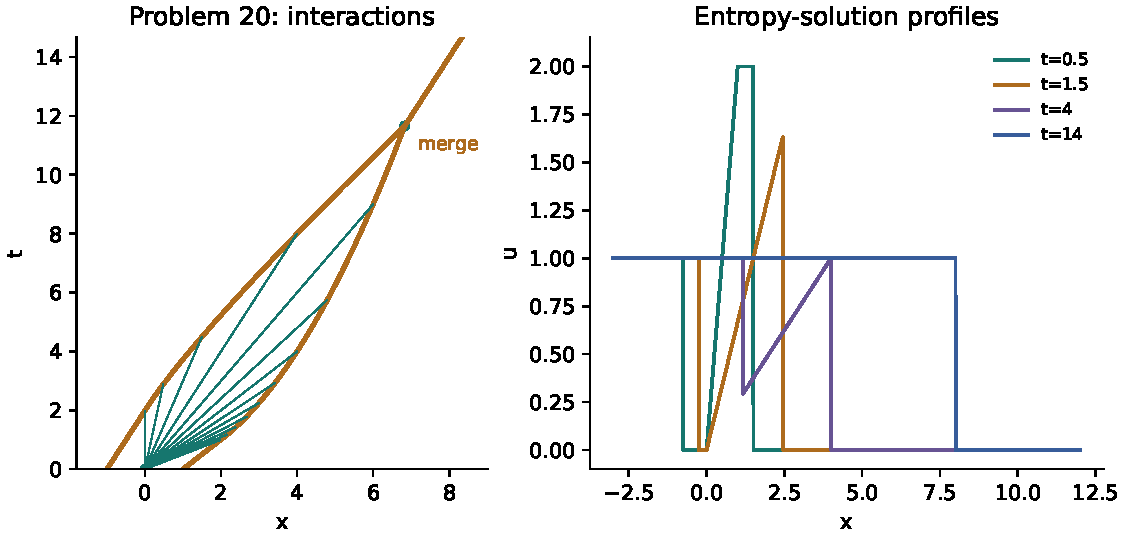
\includegraphics[width=\linewidth]{output/figures/ch03-interacting-waves.pdf}
\end{center}
\noindent\textit{Editorial figure.}
The space-time plot records interactions at $t=1$, $t=2$ and $T$;
the profiles show all four stages. Independent piecewise Hopf--Lax
minimization checks the formulas numerically away from shock ties.

% Evans second edition, section 3.6.
% English source: printed p. 158; PDF page 175 (1-based).
% Chinese section starts: checked against the chapter-opening list, PDF p. 79.
% Status: editorial study draft with detailed proofs and mathematical notes; no independent review.
\Needspace{65mm}
\section{References}
\label{sec:3-6}

The primary source is Lawrence C. Evans, \emph{Partial Differential
Equations}, second edition, Chapter 3, printed pp.~89--158
(local PDF pp.~106--175). The section order and explicit source
theorem identifiers follow that edition. The prose, expanded arguments,
Chinese notes, plots and exercise solutions are editorial reconstructions.

Evans's \S3.6 points to Courant--Hilbert for complete integrals;
Carath\'eodory, Garabedian, John, Chester and Sneddon for characteristics;
Lions, Rund and Benton for Hamilton--Jacobi theory; and Lax, Smoller
and Whitham for conservation laws.
The source attributes the HJ uniqueness argument to Douglis, the
entropy uniqueness argument to Oleinik, and the long-time estimates
to DiPerna, \emph{Indiana University Mathematics Journal} 24 (1975),
pp.~1047--1071.
These are source attributions and reading directions, not claims of
independent consultation of each listed work.

The Chinese chapter opening (PDF p.~79) lists section starts at printed
pp.~61, 64, 76, 90, 107, and 110 for \S3.1--\S3.6.
Selected Chinese pages for the local characteristic construction,
Hopf--Lax and shocks were checked as recorded in the chapter log.
A line-by-line comparison of the whole Chinese chapter has not been made.

\paragraph{Review boundary.}
The chapter invokes ODE existence and smooth dependence, implicit and
inverse function theorems, supporting hyperplanes for convex functions,
integration and weak calculus, Rademacher, and Gronwall as prerequisites.
The local existence proof includes the contact-compatibility step;
the two uniqueness arguments explicitly retain their different
selection classes. Long-time estimates are stated under convenient
sufficient convexity hypotheses, not optimal assumptions.
All 20 source exercises have solutions or exact pointers to full earlier
arguments. Numerical agreement with selected models and successful
compilation do not establish independent mathematical review.


% Source: Evans, Chapter 4, printed pp. 159--236; PDF pp. 176--253.
\chapter[Other Ways to Represent Solutions]{Other Ways to\\Represent Solutions}
\label{chap:other-ways-to-represent-solutions}
\PDESource
 {Chapter 4; printed pp.~159--236; PDF pp.~176--253}
 {中译本：第四章，书内第 111 页起；章首页 PDF 第 129 页。}
\noindent\emph{Editorial study edition.}
This chapter reconstructs the source exposition, not its wording.
Source theorem identifiers are stated separately from our numbering.
Detailed proofs, Chinese mathematical annotations, exercise solutions
and figures are editorial additions.

The organizing question is how a PDE can be represented by simpler objects:
\[
 \begin{gathered}
 \text{modes and profiles}\ \longrightarrow\ \text{integral transforms},\\
 \text{changes of unknown}\ \longrightarrow\ \text{asymptotics and power series}.
 \end{gathered}
\]
\Needspace{45mm}
\PDEAnnotation{表示公式还需要合法性}{猜到一个形式不等于已经解决问题。接着要检查初边值、可逆性、级数或积分的收敛，以及能否逐项求导；渐近展开还需另估余项。}
\paragraph{Reading conventions.}
Fourier transforms use the unitary normalization $(2\pi)^{-n/2}$.
The diffusion exponent is denoted by $m$ to distinguish it from
multiindices. A formal asymptotic calculation is identified explicitly;
its conclusion is not promoted to an unconditional convergence theorem.
We invoke standard integration, ODE theory, implicit and inverse function
theorems, and elementary complex analysis. Spectral completeness and
elliptic solvability are identified where used, rather than proved by
writing a series. Sobolev terminology is available in Chapter~5.
\clearpage
% Evans 4.1, printed pp. 159--167; PDF pp. 176--184.
% Editorial reconstruction; independent mathematical review not performed.
\Needspace{65mm}
\section{Separation of Variables}\label{sec:4-1}
\Needspace{35mm}
\subsection{Separated modes and the missing convergence question}
For $u_t-\Delta u=0$ with zero Dirichlet data on a bounded domain $U$,
try $u(x,t)=T(t)X(x)$. On a product neighborhood where both factors
are nonzero,
\[
 \frac{T'}T=\frac{\Delta X}X=-\lambda .
\]
Fixing $x$ and then $t$ shows that the common expression is constant.
The separated equations are
\[
 -\Delta X=\lambda X,\quad X|_{\partial U}=0,\qquad
 T'=-\lambda T .
\]
The identities without division continue across zeros of $X$.
For a nonzero smooth eigenfunction, integration by parts gives
\[
 \lambda\int_U|X|^2=\int_U|DX|^2>0 .
\]
Strict positivity follows since a zero-gradient function with zero
boundary trace is zero. Thus $e^{-\lambda t}X$ is a heat mode.

\Needspace{45mm}
\PDEAnnotation{分离与叠加是两步}{乘积形式只构造单个模态；把多个模态相加依赖方程的线性。非线性方程即使能分离变量，也通常不能把分离解相加来拟合任意初值。}

\PDEBodyDiagram{4.1}{A separated mode and its nodal line.}
{On the unit square, this Dirichlet mode is the product of two one-dimensional modes. The dashed line $y=1/2$ is a zero set inside the domain. Applying $-\Delta$ adds the two eigenvalues, giving $5\pi^2$; heat evolution then changes only the time factor.}
{ch04-product-mode}

\begin{theorem}[A justified spectral representation, conditional on the spectral basis]
Assume the Dirichlet eigenfunctions $X_j$ form an orthonormal basis
of $L^2(U)$, with eigenvalues $\lambda_j>0$.
For $g\in L^2(U)$, set $g_j=(g,X_j)$ and
\[
 u(\cdot,t)=\sum_{j=1}^\infty e^{-\lambda_jt}g_jX_j .
 \tag{S4}
\]
This converges in $L^2$, tends to $g$ in $L^2$ at time zero, and
solves the heat equation in the spectral weak sense.
\end{theorem}
\begin{expandedproof}
Parseval gives $\sum|g_j|^2=\|g\|_2^2$, so the tail norm squared is
at most $\sum_{j>N}|g_j|^2$, uniformly for $t\geq0$.
Moreover
\[
 \|u(t)-g\|_2^2
 =\sum_j|e^{-\lambda_jt}-1|^2|g_j|^2\longrightarrow0
\]
by dominated convergence for a summable series.
For $t\geq\tau>0$, $\sup_{\lambda\geq0}\lambda^ke^{-\tau\lambda}<\infty$.
Hence time derivatives of every order converge in $L^2$ away from zero;
the spectral Laplacian and time derivative agree termwise.
Testing against any finite eigenfunction combination proves the weak
equation, and density extends it to the corresponding energy test class.
Interior classical smoothness requires the usual elliptic/local
regularity facts; it does not follow simply from writing (S4).
Existence and completeness of the basis are the later spectral theorem
of Chapter~6, not a conclusion of separation itself.
\end{expandedproof}
On $(0,\pi)$ one has $X_j=\sqrt{2/\pi}\sin(jx)$, $\lambda_j=j^2$.
The coefficient formula is then an ordinary sine-series expansion.
A finite sum is already a classical solution for its own initial datum.

\Needspace{35mm}
\subsection{Nonlinear and additive separation}
For $u_t-\Delta(u^m)=0$, $m>1$, try $u=T(t)X(x)\geq0$.
Homogeneity gives $T'/T^m=\Delta(X^m)/X=\mu$ and therefore
\[
 T(t)=[c-(m-1)\mu t]^{-1/(m-1)},\qquad \Delta(X^m)=\mu X .
\]
Taking $X=|x|^\alpha$ and using
$\Delta r^q=q(q+n-2)r^{q-2}$ for $r>0$ yields
\[
 \alpha=\frac2{m-1},\qquad
 \mu=\alpha m(\alpha m+n-2)>0 .
\]
The positive bracket restricts the solution interval to
$t<c/((m-1)\mu)$. At the origin $X$ need not be $C^2$,
but $X^m=r^{2+2/(m-1)}$ is $C^2$ and its Laplacian extends
continuously to zero. Thus the equation holds there in this natural
sense. The profile grows at infinity and has infinite total mass.
\Needspace{45mm}
\PDEAnnotation{无穷远的条件影响物理解}{这个分离解能在有限时间爆破，但它从一开始就有无限质量。不能用它否定有限质量、紧支集数据下的扩散结论；全空间问题也要记录增长类。}
For the Hamilton--Jacobi equation, additive separation is more natural:
$u=X(x)+T(t)$ gives $H(DX)=\mu$ and $T=-\mu t+b$.
The affine choice $X=a\cdot x$ recovers the complete family of Chapter~3.

\Needspace{35mm}
\subsection{Turing instability: diffusion can destabilize a coupled system}
Let $J=D\mathbf f(0)=\left(\begin{smallmatrix}\alpha&\beta\\
\gamma&\delta\end{smallmatrix}\right)$, and
$D=\operatorname{diag}(d_1,d_2)$, $d_i>0$.
The reaction ODE is linearly asymptotically stable precisely when
\[
 \operatorname{tr}J=\alpha+\delta<0,\qquad
 \det J=\alpha\delta-\beta\gamma>0 .
\]
Indeed its two eigenvalues either are real with negative sum and
positive product, or are conjugate with negative real part.

For $\mathbf v_t-D\Delta\mathbf v=J\mathbf v$, expand in Laplacian modes.
The coefficient of $X_j$ solves
\[
 s_j'=(J-\lambda_jD)s_j .
\]
Its trace is still negative, but its determinant is
\[
 p(\lambda)=d_1d_2\lambda^2-(d_1\delta+d_2\alpha)\lambda+\det J .
\]
\begin{theorem}[Linear mode instability]
A mode grows exponentially if and only if $p(\lambda_j)<0$.
For a continuous positive instability band it is necessary and sufficient that
\[
 B=d_1\delta+d_2\alpha>0,\qquad B^2>4d_1d_2\det J .
\]
Actual instability additionally requires a domain eigenvalue in
$(\lambda_-,\lambda_+)$, where
\[
 \lambda_\pm=\frac{B\pm\sqrt{B^2-4d_1d_2\det J}}{2d_1d_2}.
\]
\end{theorem}
\begin{expandedproof}
Negative determinant gives two real eigenvalues of opposite signs.
Positive determinant and negative trace give negative real parts;
zero determinant is a neutral threshold, not strict exponential growth.
The quadratic $p$ opens upward and has positive roots exactly under
the displayed conditions. Its negative set is the interval between them.
The discrete spectrum of the chosen domain must meet this interval.
\end{expandedproof}
\Needspace{45mm}
\PDEAnnotation{连续波段不等于域内存在模态}{代数条件先给出不稳定的 $\lambda$ 区间；还要看具体区域的离散特征值是否落入其中。$p=0$ 只是临界中性情形，严格增长需要 $p<0$。}
For example, take
\[
 J=\begin{pmatrix}1&-2\\2&-3\end{pmatrix},\qquad
 D=\operatorname{diag}(0.01,1).
\]
Then $\operatorname{tr}J=-2$, $\det J=1$, while
$p(4)=0.16-3.88+1=-2.72$.
On $(0,\pi)$ the second sine mode has $\lambda_2=4$ and grows.
If $D=dI$, by contrast, every eigenvalue is shifted by $-d\lambda_j$,
so a stable $J$ remains stable.
\Needspace{45mm}
\PDEAnnotation{线性失稳不等于已证明斑图形成}{这里证明的是线性化系统存在增长模态。非线性解是否饱和、形成何种稳定空间图案，需要额外的分岔与演化理论，不能由特征值计算直接得出。}
\par\noindent\begin{minipage}{\linewidth}
\begin{center}
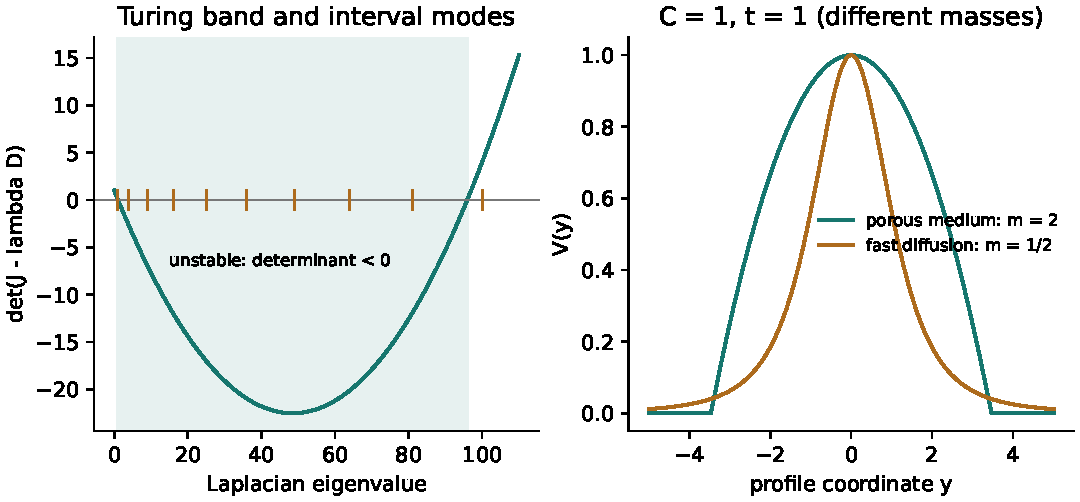
\includegraphics[width=\linewidth]{output/figures/ch04-modes-profiles.pdf}
\end{center}
\noindent\emph{Editorial figure.} The determinant band is compared with
the actual interval spectrum; the other panel compares scaling profiles.
\end{minipage}
% Evans second edition, section 4.2.
% English source: printed p. 167; PDF page 184 (1-based).
% Chinese subsection/page correspondence: pending verification against the scan.
% Status: outline-only; no source text or proof has been transcribed/reviewed.
\section{Similarity Solutions}
\label{sec:4-2}

\PDEPending

% TODO: English exposition with source theorem/equation identifiers.
% TODO: Add necessary \PDEVocab, \PDEIdea, or \PDEChinese notes.
% TODO: Expand abbreviated arguments in expandedproof/proofdetails.
% TODO: Verify hypotheses, endpoints, constants, limits, and cross-references.

% Evans 4.3.1, printed pp. 177--186; PDF pp. 194--203.
\Needspace{65mm}
\section{Transform Methods}\label{sec:4-3}
\Needspace{35mm}
\subsection{Fourier transform: normalization and Plancherel}
For $f\in L^1(\R^n)$ define
\[
 \begin{aligned}
 \widehat f(\xi)&=(2\pi)^{-n/2}\int e^{-ix\cdot\xi}f(x)\,dx,\\
 \mathcal F^{-1}h(x)&=(2\pi)^{-n/2}\int e^{ix\cdot\xi}h(\xi)\,d\xi .
 \end{aligned}
\]
The integrals are absolutely convergent.
For Schwartz functions integration by parts and Fubini yield
\[
 \widehat{\partial_j f}=i\xi_j\widehat f,\qquad
 \widehat{f*h}=(2\pi)^{n/2}\widehat f\,\widehat h .
 \tag{F4}
\]
For the second identity, set $x=z+y$ in the double integral.
Both normalizations must be retained; $\mathcal F$ is unitary,
whereas ordinary convolution has no normalizing factor.
\Needspace{45mm}
\PDEAnnotation{卷积公式为何多一个常数}{每个 Fourier 变换自带 $(2\pi)^{-n/2}$，两个变换相乘就出现两份。卷积只做一次变换，所以要乘回 $(2\pi)^{n/2}$；后面的核常数都由此决定。}


\PDEBodyDiagram{4.2}{Fourier transformation turns differentiation into multiplication.}
{The square commutes with the unitary normalization used here. There is no $2\pi$ in the multiplier because the exponential is $e^{-ix\cdot\xi}$. The heat multiplier is small at large $|\xi|$, connecting this representation with the stability picture in Chapter 1.}
{ch04-fourier-square}

\begin{theorem}[Plancherel and inversion; source Theorems 1--2]
The Fourier transform extends uniquely to a unitary operator on $L^2$.
It preserves inner products, has the displayed inverse, and
$\widehat{D^\gamma f}=(i\xi)^\gamma\widehat f$ whenever
the weak derivative is in $L^2$.
\end{theorem}
\begin{expandedproof}[Gaussian regularization without circular inversion]
\paragraph{1. The Gaussian transform.}
For $a>0$, $I(b)=\int_{\R} e^{-ax^2}e^{-ibx}\,dx$.
Differentiate under the integral and integrate by parts to get
$I'(b)=-bI(b)/(2a)$.
Since $I(0)=\sqrt{\pi/a}$,
$I(b)=\sqrt{\pi/a}\,e^{-b^2/(4a)}$.
Products give the $n$-dimensional identity.
This real-variable proof does not yet require contour deformation.

\paragraph{2. The norm identity.}
For $f\in L^1\cap L^2$ and $\eta>0$, Fubini gives
\[
 \int e^{-\eta|\xi|^2}|\widehat f(\xi)|^2\,d\xi
 =\iint f(x)\overline{f(y)}G_\eta(x-y)\,dx\,dy,
\]
where $G_\eta(z)=(4\pi\eta)^{-n/2}e^{-|z|^2/(4\eta)}$.
Fubini is legitimate since $\|f\|_1^2<\infty$ and the frequency
Gaussian is integrable.
The right side tends to $\|f\|_2^2$ because $G_\eta*f\to f$ in $L^2$.
For completeness,
\[
 \|G_\eta*f-f\|_2
 \leq\int G_\eta(z)\|f(\cdot-z)-f\|_2\,dz\longrightarrow0:
\]
translations are continuous in $L^2$ by approximation with compact
continuous functions; split the last integral into a small ball and
its Gaussian tail. Monotone convergence on the left gives the norm identity.
Polarization gives the inner-product identity.

\paragraph{3. Inversion and extension.}
For Schwartz $f$, (F4) implies rapid decay of $\widehat f$.
Fubini and the Gaussian formula give
\[
 \mathcal F^{-1}(e^{-\eta|\xi|^2}\widehat f)=G_\eta*f.
\]
The right side tends to $f$; the left tends to
$\mathcal F^{-1}\widehat f$ by dominated convergence.
Thus inversion holds on Schwartz functions.
Approximate arbitrary $L^2$ data by Schwartz functions.
The norm identity makes their transforms Cauchy and makes the limit
independent of the approximation. Inversion extends by continuity,
so the range is all of $L^2$.
Finally integration by parts against Schwartz tests proves the derivative
identity in distributions; if both sides belong to $L^2$, it is an
a.e. equality of those representatives.
\end{expandedproof}
\Needspace{45mm}
\PDEAnnotation{$L^2$ 变换不必是逐点积分}{一般 $L^2$ 函数未必可积，其 Fourier 变换通过范数极限定义。反演和乘子公式首先是 $L^2$ 等式；若要逐点表示，还须增加可积性或正则性。}

\Needspace{35mm}
\subsection{Fourier multipliers and evolution equations}
\paragraph{Bessel potential.}
For $-\Delta u+u=f$, $f\in L^2$,
$\widehat u=(1+|\xi|^2)^{-1}\widehat f$.
This gives a unique $L^2$ distributional solution with
$\int(1+|\xi|^2)^2|\widehat u|^2<\infty$.
A rigorous kernel representation is
\[
 K(x)=\int_0^\infty e^{-s}G_s(x)\,ds,\qquad u=K*f .
\]
Tonelli gives $K\geq0$ and $\|K\|_1=1$;
its transform is $(2\pi)^{-n/2}/(1+|\xi|^2)$.
The kernel called $B$ in the source is $(2\pi)^{n/2}K$.
The singularity of $K$ at zero in some dimensions does not prevent
its $L^1$ integrability or convolution action on $L^2$.
\Needspace{45mm}
\PDEAnnotation{乘子有界不表示核处处有限}{$(1+|\xi|^2)^{-1}$ 给出有界的 $L^2$ 乘子。对应核可能在原点无界，但仍可积；不能把一个点的奇性误当作表示公式失效。}

\paragraph{Heat and Schr\"odinger equations.}
Spatial transformation of $u_t-\Delta u=0$ gives
$\widehat u_t+|\xi|^2\widehat u=0$, hence
$\widehat u=e^{-t|\xi|^2}\widehat g$.
Gaussian inversion recovers $u=G_t*g$ from Chapter~2.
For $iu_t+\Delta u=0$ the sign is instead
$\widehat u_t=-i|\xi|^2\widehat u$, so
\[
 \widehat u=e^{-it|\xi|^2}\widehat g,\qquad
 u(x,t)=(4\pi it)^{-n/2}\int e^{i|x-y|^2/(4t)}g(y)\,dy .
 \tag{SC4}
\]
For $t\ne0$ use
$(it)^{-n/2}=|t|^{-n/2}e^{-i\pi n\,\operatorname{sgn}(t)/4}$.
The kernel identity follows by first replacing $it$ with $\eta+it$,
$\eta>0$, and then letting $\eta\downarrow0$.
For $g\in L^1\cap L^2$, the kernels converge under the spatial integral
by domination, while the multipliers converge in $L^2$.
Thus both descriptions agree.
For $L^2$ data this defines a unitary group:
\[
 \|u(t)\|_2=\|g\|_2,\qquad
 \|u(t)-g\|_2^2
 =\int|e^{-it|\xi|^2}-1|^2|\widehat g|^2\longrightarrow0 .
\]
If $g,|x|^2g\in L^1$, differentiation of (SC4) on compact
space-time sets away from $t=0$ verifies the classical PDE.
For arbitrary $L^2$ data the statement is distributional.
\Needspace{45mm}
\PDEAnnotation{色散与耗散的范数表现不同}{热乘子模长小于一，会压低高频；Schr\"odinger 乘子模长为一，保持 $L^2$。后者的点态衰减来自振荡抵消，不来自 $L^2$ 质量损失。}

\paragraph{Wave and telegraph equations.}
For $u_{tt}-\Delta u=0$, $u(0)=g$, $u_t(0)=h$,
\[
 \widehat u(\xi,t)=\cos(t|\xi|)\widehat g
              +\frac{\sin(t|\xi|)}{|\xi|}\widehat h.
 \tag{WV4}
\]
At $\xi=0$ the quotient is defined as $t$.
It is bounded by $t$, so the formula has no genuine zero-frequency pole.
For $u_{tt}+2du_t-u_{xx}=0$ use $\widehat u=e^{-dt}v$.
Then $v''+(\xi^2-d^2)v=0$ and
\[
 \widehat u=e^{-dt}
 \begin{cases}
 \cosh(qt)\widehat g+\dfrac{\sinh(qt)}q(\widehat h+d\widehat g),
                 &|\xi|<d,\ q=\sqrt{d^2-\xi^2},\\
 \widehat g+t(\widehat h+d\widehat g),&|\xi|=d,\\
 \cos(qt)\widehat g+\dfrac{\sin(qt)}q(\widehat h+d\widehat g),
                 &|\xi|>d,\ q=\sqrt{\xi^2-d^2}.
 \end{cases}
\]
These are the overdamped, critical and oscillatory regimes.
The common limiting formula at $q=0$ is essential.

\begin{theorem}[Asymptotic energy equipartition; source \S4.3.1]
If $g\in H^1(\R^n)$ and $h\in L^2(\R^n)$, the wave solution has
\[
 \|Du(t)\|_2^2\longrightarrow E_0,\qquad
 \|u_t(t)\|_2^2\longrightarrow E_0,\qquad
 E_0=\tfrac12(\|Dg\|_2^2+\|h\|_2^2).
\]
\end{theorem}
\begin{expandedproof}
Write $A=|\xi|\widehat g$ and $B=\widehat h$ in $L^2$.
Plancherel and (WV4) give
\[
 \|Du\|_2^2
 =\int|A|^2\cos^2(t|\xi|)+|B|^2\sin^2(t|\xi|)
       +2\operatorname{Re}(A\overline B)\sin(t|\xi|)\cos(t|\xi|).
\]
All three coefficient functions are $L^1$, the cross term by
Cauchy--Schwarz.
For any $F\in L^1(\R^n)$, polar coordinates give
$\int e^{2it|\xi|}F(\xi)\,d\xi=\int_0^\infty e^{2itr}H(r)\,dr$
with $\|H\|_1\leq\|F\|_1$.
The latter tends to zero: approximate $H$ in $L^1$ by smooth functions
supported inside $(0,\infty)$ and integrate those by parts.
Now use the double-angle identities to obtain the first limit.
The analogous formula for $u_t$ gives energy conservation and
the second limit.
This also handles $n=1$ without discarding a possible endpoint term
in a radial integration by parts.
\end{expandedproof}
\input{chapters/04-other-ways-to-represent-solutions/03a-radon-laplace}

% Evans second edition, section 4.4.
% English source: printed p. 195; PDF page 212 (1-based).
% Chinese subsection/page correspondence: pending verification against the scan.
% Status: outline-only; no source text or proof has been transcribed/reviewed.
\section{Converting Nonlinear into Linear PDE}
\label{sec:4-4}

\PDEPending

% TODO: English exposition with source theorem/equation identifiers.
% TODO: Add necessary \PDEVocab, \PDEIdea, or \PDEChinese notes.
% TODO: Expand abbreviated arguments in expandedproof/proofdetails.
% TODO: Verify hypotheses, endpoints, constants, limits, and cross-references.

% Evans 4.5.1--2, printed pp. 200--206; PDF pp. 217--223.
\Needspace{65mm}
\section{Asymptotics}\label{sec:4-5}
The source presents several asymptotic constructions formally.
We distinguish exact algebraic identities, proved local integral
asymptotics, and conditional PDE expansions.
No convergence theorem is inferred merely by matching powers.

\Needspace{35mm}
\subsection{A small-diffusion plume: geometry and transverse scale}
Consider $\operatorname{div}(\mathbf b\,\mu)=\delta_0$ in two dimensions.
Let $\dot X=\mathbf b(X)$, $X(0)=0$, and suppose $|\mathbf b(X)|>0$.
If the forward trajectory leaves compact sets, the locally finite measure
\[
 \int\phi\,d\mu=\int_0^\infty\phi(X(t))\,dt
\]
solves this equation, since
\[
 -\int\mathbf b\cdot D\phi\,d\mu
 =-\int_0^\infty\frac d{dt}\phi(X(t))\,dt=\phi(0).
\]
This is an outgoing solution; an extra background homogeneous solution
is not excluded by this calculation.
With speed $\sigma=|\mathbf b(X)|$, tangent $\tau$ and unit normal $\nu$,
use $x=X(t)+y\nu(t)$ in a nonoverlapping tubular neighborhood.
Frenet identities give $\nu'=-\sigma\kappa\tau$ and
\[
 x_t=\sigma(1-\kappa y)\tau,\quad x_y=\nu,\quad
 dx=H\,dt\,dy,\qquad H=\sigma(1-\kappa y)>0.
\]
Thus the same measure has density $\delta(y)/\sigma(t)$ with respect
to spatial area.
\Needspace{45mm}
\PDEAnnotation{线上的密度必须带速度因子}{注入量按行进时间计量，而面积元在曲线处含 $\sigma(t)$。因此横向 Dirac 前要乘 $1/\sigma$。若轨道封闭或反复回返，时间积分可能不是局部有限测度。}

Now perturb to $-\varepsilon\Delta u^\varepsilon+
\operatorname{div}(\mathbf b u^\varepsilon)=\delta_0$.
Away from the injection point, set
$z=y/\sqrt\varepsilon$,
$u^\varepsilon=\varepsilon^{-1/2}v^\varepsilon(t,z)$.
The coordinate metric gives the exact identity
\[
 \Delta w=\frac1H\partial_t(H^{-1}w_t)
                  +\frac1H\partial_y(Hw_y).
\]
Also write
$\mathbf b=(\sigma+\alpha y+O(y^2))\tau+
(\beta y+O(y^2))\nu$.
Then on compact $t>0$, bounded $z$, provided the needed derivatives
of $v^\varepsilon$ are uniformly bounded,
\[
 \mathbf b\cdot Dv^\varepsilon
       =v^\varepsilon_t+\beta z v^\varepsilon_z+O(\sqrt\varepsilon),
 \qquad
 \varepsilon\Delta v^\varepsilon=v^\varepsilon_{zz}+O(\sqrt\varepsilon),
\]
\[
 \operatorname{div}\mathbf b
       =\sigma'/\sigma+\beta+O(\sqrt\varepsilon).
\]
For example the transverse first-derivative term in the Laplacian
is $\varepsilon(H_y/H)\partial_yv^\varepsilon=O(\sqrt\varepsilon)$;
the tangential second-derivative terms are $O(\varepsilon)$.
Thus the conditional leading equation is
\[
 v_t-v_{zz}+(\beta z v)_z+(\sigma'/\sigma)v=0,\qquad
 v(0)=\delta_0/\sigma(0).
 \tag{PL4}
\]
Its exact Gaussian solution, derived again in Problem 13, is
\[
 v(t,z)=\frac{e^{-z^2/\Gamma(t)}}{\sigma(t)\sqrt{\pi\Gamma(t)}},
 \qquad \Gamma'=4+2\beta\Gamma,\quad\Gamma(0)=0 .
\]
Indeed $A=\sigma v$ satisfies $A_t=A_{zz}-(\beta zA)_z$;
substituting the Gaussian gives the displayed ODE and mass $\int A=1$.
The transverse width is $\sqrt{\varepsilon\Gamma(t)}$.
This does not by itself prove approximation of the original elliptic
Green function, nor control the injection region or large times.
\Needspace{45mm}
\PDEAnnotation{形式余项依赖尚未证明的统一界}{把 $y$ 换成 $\sqrt\varepsilon z$ 后，系数误差很小，但它仍乘着解的导数。只有这些导数在所考察区域有统一界，才能写成统一的 $O(\sqrt\varepsilon)$。}

\Needspace{35mm}
\subsection{Laplace concentration and vanishing viscosity}\label{sec:4-laplace}
\begin{lemma}[Source asymptotics lemma, with tail control]
Let $k,l$ be continuous on $\R$, $|l(y)|\leq C(1+|y|)$,
and $k(y)\geq c y^2-C$, $c>0$.
If $k$ has a unique minimum at $y_0$, then
\[
 \frac{\int l(y)e^{-k(y)/\varepsilon}\,dy}
      {\int e^{-k(y)/\varepsilon}\,dy}\longrightarrow l(y_0).
 \tag{LC4}
\]
\end{lemma}
\begin{expandedproof}
Subtract the minimum $k_0$ and put $h=k-k_0\geq0$.
Fix a small neighborhood $N$ of $y_0$ on which
$|l-l(y_0)|<\eta$.
On a large compact interval outside $N$, $h\geq d>0$ by uniqueness.
Increase the interval so that outside it
$h(y)\geq d/2+(c/2)y^2$, decreasing $d$ if necessary.
By continuity there is an interval of length $2r>0$ near $y_0$
where $h<d/4$.
The denominator is at least $2r e^{-d/(4\varepsilon)}$.
The numerator of the absolute error over the compact complement
is at most $C_1e^{-d/\varepsilon}$.
The tail numerator is bounded by
\[
 C_2e^{-d/(2\varepsilon)}
       \int(1+|y|)e^{-cy^2/(2\varepsilon)}\,dy,
\]
whose ratio to the denominator tends to zero.
Inside $N$ the normalized error is at most $\eta$.
Let $\varepsilon\downarrow0$ and then $\eta\downarrow0$.
This proves concentration together with the required control of
the unbounded observable $l$.
\end{expandedproof}
\Needspace{45mm}
\PDEAnnotation{逐点密度趋零不足以推出集中}{归一化密度在每个非极小点趋零，还不能控制积分或无穷远的质量。证明需要分母下界、远离极小点的能量间隙，以及带权尾积分。}

For bounded initial $g$, let $P'=g$ and
$K(y)=(x-y)^2/(2t)+P(y)$.
The quadratic term dominates the Lipschitz primitive.
Formula (VB4) and (LC4), with parameter $2\varepsilon$, imply
\[
 u^\varepsilon(x,t)\longrightarrow \frac{x-y(x,t)}t
\]
whenever the minimizing point is unique.
By Chapter~3, at each $t>0$ only countably many $x$ have multiple
minimizers, and the right side is the Lax--Oleinik entropy solution.
Since $|u^\varepsilon|\leq\|g\|_\infty$, this convergence is also
$L^1_{\rm loc}$ in $x$ for each fixed $t$.
Joint a.e. convergence and the same bound give local space-time
$L^1$ convergence away from zero.
The multiple-minimizer set is measurable, for instance by expressing
separation of two minimizers using rational compact neighborhoods;
Fubini therefore applies to the countable time slices.
\Needspace{45mm}
\PDEAnnotation{与第三章的最小化公式接上了}{黏性解是最优速度的指数加权平均。黏性趋零时，权重集中到作用量最低点；最低点的分支竞争正对应守恒律的激波。}

If $k$ is smooth with finitely many nondegenerate global minima $y_j$,
local Taylor expansion $y=y_j+\sqrt\varepsilon z$ and Gaussian
domination give
\[
 \int l e^{-k/\varepsilon}
 =e^{-k_0/\varepsilon}\sqrt{2\pi\varepsilon}
       \left(\sum_j\frac{l(y_j)}{\sqrt{k''(y_j)}}+o(1)\right).
\]
To justify domination, restrict to a small neighborhood where
$k-k_0\geq c_j|y-y_j|^2$, and use the energy gap outside.
Thus at a tie the limit is a weighted average, not necessarily
the velocity at one selected minimizing point.
Values on shock curves do not affect the weak solution.
\input{chapters/04-other-ways-to-represent-solutions/05a-stationary-phase}
\input{chapters/04-other-ways-to-represent-solutions/05b-homogenization}
% Evans second edition, section 4.6.
% English source: printed p. 220; PDF page 237 (1-based).
% Chinese subsection/page correspondence: pending verification against the scan.
% Status: outline-only; no source text or proof has been transcribed/reviewed.
\section{Power Series}
\label{sec:4-6}

\PDEPending

% TODO: English exposition with source theorem/equation identifiers.
% TODO: Add necessary \PDEVocab, \PDEIdea, or \PDEChinese notes.
% TODO: Expand abbreviated arguments in expandedproof/proofdetails.
% TODO: Verify hypotheses, endpoints, constants, limits, and cross-references.

% Evans 4.7, Problems 1--19, printed pp. 231--236; PDF pp. 248--253.
\Needspace{65mm}
\section{Problems}\label{sec:4-7}
\noindent\emph{Source: Evans \S4.7, Problems 1--19.}
Statements are restated concisely; all solutions and domain
clarifications below are editorial.

\Needspace{35mm}
\subsection{Separation, scaling and traveling profiles}
\Needspace{30mm}
\paragraph{1. Aronsson's infinity-harmonic example.}
\begin{proof}[Solution]
For $u=f(x)+g(y)$, the equation is
$(f')^2f''+(g')^2g''=0$.
Set these terms equal to $64/81$ and $-64/81$ respectively.
A resulting profile is
\[
 u(x,y)=|x|^{4/3}-|y|^{4/3}.
\]
Off the axes, $(f')^2f''=64/81$ and
$(g')^2g''=-64/81$, so the PDE holds classically there.
The function is $C^1$ on $\R^2$ but not $C^2$ on the axes.
It is a global viscosity solution of
$F(Du,D^2u)=-Du\cdot D^2u\,Du=0$, as follows.

At $x=0$, $y\ne0$, no $C^2$ function touches $u$ from above:
the positive $|x|^{4/3}$ increment is larger than every quadratic
with zero first derivative at zero.
For a test $\phi$ touching from below, $D\phi=Du$ and
$\phi_{yy}\leq u_{yy}<0$, so
$D\phi\cdot D^2\phi D\phi\leq0$, giving $F\geq0$.
At $y=0$, $x\ne0$ the lower tests are absent, while an upper test has
$\phi_{xx}\geq u_{xx}>0$ and hence $F\leq0$.
At the origin every touching test has gradient zero, and $F=0$.
These are exactly the viscosity inequalities.
An affine function supplies a global classical solution if that
solution class is required; the nonaffine Aronsson example needs the
explicit weaker interpretation.
\end{proof}
\Needspace{45mm}
\PDEAnnotation{经典解与黏性解要分清}{$|x|^{4/3}-|y|^{4/3}$ 不能在坐标轴上按经典二阶导数代入。本题用接触测试说明它的全局解意义；黏性解的一般理论留待第十章。}

\Needspace{30mm}
\paragraph{2. Hadamard instability of Laplace Cauchy data.}
\begin{proof}[Solution]
The separated ansatz $\sin(nx_1)T(x_2)$ gives $T''=n^2T$.
The data $T(0)=0$, $T'(0)=1/n$ yield
\[
 u_n(x_1,x_2)=n^{-2}\sin(nx_1)\sinh(nx_2).
\]
The Cauchy data tend uniformly to zero, but on any line $x_2=h>0$,
$\sup_{x_1}|u_n|=n^{-2}\sinh(nh)\to\infty$.
Thus the data-to-solution map is not continuous in these uniform
data and solution norms. One must not claim pointwise divergence
at every fixed $x_1$, since $\sin(nx_1)$ can vanish.
Existence of analytic solutions does not restore this stability.
\end{proof}

\Needspace{30mm}
\paragraph{3. A balanced bistable front.}
\begin{proof}[Solution]
For $f(v)=-2v^3+3v^2-v$, $\int_0^1f=0$.
The energy identity (BF4) forces speed $c=0$ for a nonconstant front.
Here $F(v)=-v^2(1-v)^2/2$, so
$(v')^2=v^2(1-v)^2$ and the increasing branch obeys $v'=v(1-v)$.
Hence $v(s)=(1+e^{-(s-s_0)})^{-1}$.
It has the required endpoints and vanishing derivatives.
Its second derivative is $v(1-v)(1-2v)=-f(v)$,
verifying the ODE directly.
\end{proof}

\Needspace{30mm}
\paragraph{4. Emden--Fowler coordinates.}
\begin{proof}[Solution]
Put $a=2/(p-1)$, $t=\log r$, and $X(t)=e^{at}v(e^t)$.
Then
\[
 v'=r^{-a-1}(X'-aX),\quad
 v''=r^{-a-2}\{X''-(2a+1)X'+a(a+1)X\}.
\]
Since $ap=a+2$, the radial equation becomes the autonomous ODE
\[
 X''+(n-2-2a)X'+a(a-n+2)X+X^p=0.
\]
This change treats $r>0$; regularity at the center is an additional
condition corresponding to $t\to-\infty$.
\end{proof}

\Needspace{30mm}
\paragraph{5. Fast-diffusion scaling profile.}
\begin{proof}[Solution]
In the standard parabolic range $\max\{0,(n-2)/n\}<m<1$, use
$\beta=1/(n(m-1)+2)>0$, $\alpha=n\beta$ as in \S4.2.
Integrating $(W^m)'=-\beta rW$ gives
\[
 u(x,t)=t^{-\alpha}
 \left(C+\frac{(1-m)\beta}{2m}|x|^2t^{-2\beta}\right)^{-1/(1-m)},
 \qquad C>0.
\]
It is positive and smooth at every $t>0$.
Its spatial tail is $|x|^{-2/(1-m)}$; integrability is equivalent to
$2/(1-m)>n$, the stated mass-critical lower bound.
Directly differentiating $W^{m-1}=C+(1-m)\beta r^2/(2m)$ verifies
the profile ODE.
Unlike the porous-medium profile it has no compact support.
If $n=1$, the source's written bound $(n-2)/n<m<1$ alone
also permits $m\leq0$. The above forward diffusion construction uses
$m>0$; it does not assert a decaying positive profile for those
nonparabolic exponents. At $m=0$ the positive equation is $u_t=0$,
a separate degeneracy.
\end{proof}
\Needspace{45mm}
\PDEAnnotation{快扩散仍需正的扩散指数}{扩散系数为 $m u^{m-1}$。$0<m<1$ 时在低密度处很大，产生代数尾；若 $m<0$，最高阶符号反转，已不是同一类前向抛物扩散。}

\Needspace{30mm}
\paragraph{6. A boundary blowup solution.}
\begin{proof}[Solution]
Assume $n\geq3$ and set $p=(n+2)/(n-2)$.
For $u=A(1-r^2)^{-b}$, radial differentiation gives
\[
 \Delta u=2bA(1-r^2)^{-b-2}
                 \{n+(2b+2-n)r^2\}.
\]
Choose $b=(n-2)/2$ so the brace is $n$ and $bp=b+2$.
Then $-\Delta u+u^p=0$ if
\[
 A=[n(n-2)]^{(n-2)/4}.
\]
This is smooth and finite in the open ball but diverges at every
boundary point, as required.
\end{proof}

\Needspace{30mm}
\paragraph{7. Viscous shock profiles and the entropy direction.}
\begin{proof}[Solution]
For $u_t+F(u)_x-au_{xx}=0$ put $u=v(x-ct)$.
Integration yields
\[
 av'=F(v)-cv+b=:Q(v).
\]
Separation gives $s=\int_{v(0)}^{v(s)}a/Q(z)\,dz$ wherever $Q\ne0$.
A connection from $u_l$ to $u_r$ forces both endpoint values of $Q$
to vanish; otherwise $v'$ stays away from zero near that endpoint
and $v$ cannot have the asserted limit.
Subtracting the endpoint identities gives
$c=(F(u_l)-F(u_r))/(u_l-u_r)$.
Conversely, for $u_l>u_r$, strict convexity makes
$Q<0$ on $(u_r,u_l)$ when $b$ is chosen to make the endpoints zero.
The zeros are simple: $Q'(u_r)<0<Q'(u_l)$.
The integral therefore diverges to $+\infty$ as $v\downarrow u_r$
and to $-\infty$ as $v\uparrow u_l$.
Its inverse is the decreasing heteroclinic profile, unique up to shift.

Normalize $v^\varepsilon(0)=(u_l+u_r)/2$.
Then $v^\varepsilon(s)=v^1(s/\varepsilon)$.
For $x-ct<0$ its limit is $u_l$, for $x-ct>0$ it is $u_r$,
and on $x=ct$ it is the chosen midpoint.
Boundedness gives local $L^1$ convergence to the Rankine--Hugoniot
downward shock. The viscous connection thus selects the entropy direction.
\end{proof}

\Needspace{35mm}
\subsection{Transforms and linearization}
\Needspace{30mm}
\paragraph{8. Schr\"odinger dispersive bound.}
\begin{proof}[Solution]
For $g\in L^1$, the modulus of the kernel in (SC4) is
$(4\pi|t|)^{-n/2}$. The triangle inequality gives
$\|u(t)\|_\infty\leq(4\pi|t|)^{-n/2}\|g\|_1$.
The bound holds for both signs of $t\ne0$.
It is consistent with conservation of the $L^2$ norm, since the
norms measure different features.
\end{proof}

\Needspace{30mm}
\paragraph{9. Inverting a nonlinear heat equation.}
\begin{proof}[Solution]
For $y=u(x,t)$, $x=v(y,t)$ and $u_x>0$, differentiate
$u(v(y,t),t)=y$:
\[
 u_x=1/v_y,\quad u_t=-v_t/v_y,\quad u_{xx}=-v_{yy}/v_y^3.
\]
Substitution into $u_t=u_{xx}/u_x^2$ gives $v_t=v_{yy}$.
This is local in the range of $u$; the inverse's spatial interval
and boundary conditions may move with time.
\end{proof}

\Needspace{30mm}
\paragraph{10. A local transformation to Liouville's equation.}
\begin{proof}[Solution]
Taken literally for every solution $u$ with a smooth real
$f:\R^3\to\R$, the request is impossible: constant $u$ would give
constant $w=f(u,0,0)$, while $w_{xt}=e^w>0$.
The intended transformation must be local on a nondegenerate branch.

For $u_{xt}=0$, write $u=A(x)+B(t)$.
On $u\ne0$, $u_xu_t>0$, choose
\[
 w=f(u,u_x,u_t)=\log(2u_xu_t/u^2)
        =\log2+\log|u_x|+\log|u_t|-2\log|u|.
\]
The first two derivative terms have zero mixed derivative, while
\[
 (-2\log|u|)_{xt}=2u_xu_t/u^2=e^w .
\]
This verifies the transformation on its real domain.
More generally, for an additive ansatz $f=a(z)+b(p)+c(q)$,
the mixed derivative equals $a''(u)u_xu_t$,
which explains the logarithmic separation.
\end{proof}
\Needspace{45mm}
\PDEAnnotation{变换的定义域不能隐去}{本题对数公式只在 $u\ne0$ 且 $u_xu_t>0$ 的分支上成立。常数解给出一个直接检查：不存在对所有三元输入光滑、又能转换所有解的实函数。}

\Needspace{30mm}
\paragraph{11. Lax pairs preserve a smooth eigenvalue branch.}
\begin{proof}[Solution]
Differentiate $Lw=\lambda w$ and take the real Hilbert inner
product with $w\ne0$.
Symmetry of $L$ cancels the two $w_t$ terms, leaving
$\lambda'\|w\|^2=(L_tw,w)$.
If $L_t=BL-LB$, then
\[
 (L_tw,w)=\lambda(Bw,w)-(Bw,Lw)=0.
\]
Thus $\lambda'=0$.
For unbounded operators all these pairings require a common
suitable domain and the differentiability stipulated by the exercise;
formal operator symbols alone do not supply these hypotheses.
\end{proof}

\Needspace{30mm}
\paragraph{12. The KdV commutator.}
\begin{proof}[Solution]
Let $D=\partial_x$, $L=-D^2+u$,
$B=-4D^3+6uD+3u_x$.
Using $D(av)=aDv+a_xv$ gives
\[
\begin{aligned}
 [-4D^3,u]&=-12u_xD^2-12u_{xx}D-4u_{xxx},\\
 [6uD,-D^2]&=12u_xD^2+6u_{xx}D,\\
 [3u_x,-D^2]&=6u_{xx}D+3u_{xxx},\\
 [6uD,u]&=6uu_x .
\end{aligned}
\]
All derivative terms cancel, leaving $[B,L]=-u_{xxx}+6uu_x$.
Since $L_t$ is multiplication by $u_t$,
$(L_t-[B,L])v=(u_t+u_{xxx}-6uu_x)v$.
For a KdV solution, every eigenvalue branch meeting Problem 11's
operator hypotheses is constant.
This is a conditional spectral conclusion, not a domain-free proof
about every possible realization of the differential expression.
\end{proof}

\Needspace{35mm}
\subsection{Asymptotics, homogenization and analytic obstructions}
\Needspace{30mm}
\paragraph{13. The plume's Gaussian width.}
\begin{proof}[Solution]
Set $A=\sigma v$ in (PL4). Then
$A_t-A_{zz}+(\beta zA)_z=0$ and $A(0)=\delta_0$.
For $A=(\pi\Gamma)^{-1/2}e^{-z^2/\Gamma}$,
\[
 A_t/A=-\Gamma'/(2\Gamma)+z^2\Gamma'/\Gamma^2,\quad
 A_{zz}/A=-2/\Gamma+4z^2/\Gamma^2.
\]
Also $(\beta zA)_z/A=\beta-2\beta z^2/\Gamma$.
Both coefficients vanish precisely when
$\Gamma'=4+2\beta\Gamma$, with $\Gamma(0)=0$ for the point-mass trace.
Hence
\[
 \Gamma(t)=4e^{2\int_0^t\beta(r)\,dr}
                \int_0^te^{-2\int_0^s\beta(r)\,dr}\,ds>0 .
\]
The normalized Gaussian has mass one and converges weakly to $\delta_0$,
verifying the initial condition after division by $\sigma$.
\end{proof}

\Needspace{30mm}
\paragraph{14. A relaxation system produces logarithmic diffusion.}
\begin{proof}[Solution]
Write the equations as
$u_t^\varepsilon+\varepsilon^{-1}u_x^\varepsilon
=\varepsilon^{-2}((v^\varepsilon)^2-(u^\varepsilon)^2)$
and the opposite equation for $v^\varepsilon$.
Multiplying by $\varepsilon^2$ and using the assumed bounded
remainders yields $(u^0)^2=(v^0)^2$.
Positivity forces $u^0=v^0=w$.

Define the bounded corrections
$U^\varepsilon=(u^\varepsilon-w)/\varepsilon$ and
$V^\varepsilon=(v^\varepsilon-w)/\varepsilon$;
the source's remainder is only assumed to be order $\varepsilon$.
The first equation, multiplied by $\varepsilon$, gives
\[
 (V^\varepsilon-U^\varepsilon)(u^\varepsilon+v^\varepsilon)
       =u_x^\varepsilon+\varepsilon u_t^\varepsilon.
\]
On compact sets $w>0$, so the denominator stays positive and
$V^\varepsilon-U^\varepsilon\to w_x/(2w)$ locally uniformly.
Adding the two original equations gives
\[
 u_t^\varepsilon+v_t^\varepsilon
                 +\partial_x(U^\varepsilon-V^\varepsilon)=0 .
\]
Pass to the limit in distributions, using the uniform derivative
bounds in the hypotheses. The result is
$2w_t-\partial_x(w_x/(2w))=0$, or
\[
 w_t-\tfrac14(\log w)_{xx}=0 .
\]
No separate limit of the two first-order corrections is needed.
\end{proof}
\Needspace{45mm}
\PDEAnnotation{只能按实际余项阶数做比较}{若余项仍是 $\varepsilon$ 乘一个有界函数，就不能把固定的 $u_1,v_1$ 自动认作唯一一阶系数。证明直接控制两者的差，再用两方程之和取极限。}

\Needspace{30mm}
\paragraph{15. Gaussian contour deformation.}
\begin{proof}[Solution]
For $q=\delta-i\lambda$, $\delta>0$, the completed-square variable
puts the contour on a translated line $e^{i\theta}\R+c$,
where $\theta=\arg\sqrt q$ satisfies $|\theta|<\pi/4$.
First remove the translation: close the two parallel line segments
at parameters $\pm R$ by segments of bounded length.
On those connectors
$\operatorname{Re}z^2\geq R^2\cos(2\theta)-C R-C$,
so their integrals of $e^{-z^2}$ tend to zero.
Cauchy's theorem equates the two infinite line integrals.

Then rotate $e^{i\theta}\R$ onto $\R$.
On connecting arcs of radius $R$ within the fixed sector,
$|e^{-z^2}|\leq e^{-R^2\cos(2\theta)}$; their length is $O(R)$,
so they also vanish. The integral is $\sqrt\pi$ with the inherited
orientation.
This argument holds for each fixed $\delta>0$;
the limiting Fresnel branch is obtained afterward, not by claiming
uniform decay on a sector boundary where the cosine is zero.
\end{proof}

\Needspace{30mm}
\paragraph{16. Schr\"odinger initial recovery.}
\begin{proof}[Solution]
For $g\in C_c^\infty$, apply (SP4) to
$\phi(y)=|x-y|^2/4$ with parameter $t>0$.
Its sole critical point is $y=x$ and Hessian is $I/2$.
The factor $(4\pi t)^{n/2}e^{i\pi n/4}$ from stationary phase
cancels the prefactor in (SC4), so $u(x,t)=g(x)+O(t)$,
uniformly for $x$ in compact sets.
For general $g\in L^2$, the multiplier and dominated convergence give
$u(t)\to g$ strongly in $L^2$, as proved in \S4.3.
One cannot replace this by absolute-integral approximate-identity
theory for a positive kernel: the Schr\"odinger kernel is oscillatory
and is not in $L^1$ as a function of space.
\end{proof}

\Needspace{30mm}
\paragraph{17. One-dimensional effective coefficient.}
\begin{proof}[Solution]
Set $F(x)=\int_0^xf(s)\,ds$ and $b=1/a$.
Integration of the flux equation gives
\[
 (u^\varepsilon)'=b(x/\varepsilon)(C_\varepsilon-F(x)),\qquad
 C_\varepsilon=
 \frac{\int_0^1b(x/\varepsilon)F(x)\,dx}
      {\int_0^1b(x/\varepsilon)\,dx}.
\]
The boundary condition $\int_0^1(u^\varepsilon)'=0$
determines this constant.
Periodic averaging gives $b(x/\varepsilon)\rightharpoonup^*\langle b\rangle$,
$C_\varepsilon\to C=\int_0^1F$.
The formula is uniformly bounded in $L^2$, and its weak limit is
$u'=\langle b\rangle(C-F)$.
The zero traces and uniqueness identify the weak $H_0^1$ limit, with
$-\overline a\,u''=f$, $\overline a=\langle1/a\rangle^{-1}$.
For the cell problem, $a(1-\chi')$ is constant;
integrating $\chi'=1-\overline a/a$ over a period yields exactly
the same harmonic mean.
\end{proof}

\Needspace{30mm}
\paragraph{18. Primal and dual variational principles.}
\begin{proof}[Solution]
All averages use the unit cube, of volume one.
For $\chi_\xi=\sum\xi_i\chi_i$, the cell orthogonality proves
\[
 \xi\cdot\overline A\xi
 =\min_{v\ {\rm periodic}}\int_Q(\xi+Dv)\cdot A(\xi+Dv),
\]
with minimizer $v=-\chi_\xi$.
For the dual problem fix $\eta$ and set
$\xi=\overline A^{-1}\eta$,
$\sigma_*=A(\xi-D\chi_\xi)$.
It is periodic, divergence free and has mean $\eta$.
For any admissible $\sigma=\sigma_*+\tau$, $\int_Q\tau=0$ and
$\operatorname{div}\tau=0$, so periodic integration by parts gives
\[
 \int_Q\tau\cdot A^{-1}\sigma_*
 =\int_Q\tau\cdot(\xi-D\chi_\xi)=0 .
\]
Expansion of the square therefore shows that $\sigma_*$ minimizes
$\int_Q\sigma\cdot A^{-1}\sigma$, with minimum
$\xi\cdot\overline A\xi=\eta\cdot\overline A^{-1}\eta$.

The primal competitor $v=0$ gives $\overline A\leq\int_QA$.
The constant dual competitor $\sigma=\eta$ gives
$\overline A^{-1}\leq\int_QA^{-1}$.
Inverting positive definite matrices reverses this order
(conjugate by a square root and diagonalize), so
\[
 \left(\int_QA^{-1}\right)^{-1}\leq\overline A\leq\int_QA .
\]
These are quadratic-form inequalities, not entrywise inequalities.
\end{proof}

\Needspace{30mm}
\paragraph{19. Analytic initial data need not give a time-analytic heat solution.}
\begin{proof}[Solution]
The total-order-two principal polynomial of $u_t-u_{xx}$ is $-\xi^2$.
At the normal to $\{t=0\}$, $(\xi,\tau)=(0,1)$, it vanishes.
Thus this is a characteristic surface for the CK theorem.

If a solution with $u(x,0)=1/(1+x^2)$ were analytic near $(0,0)$,
the PDE would give
\[
 \partial_t^ku(0,0)=\partial_x^{2k}(1+x^2)^{-1}|_{x=0}
                 =(-1)^k(2k)! .
\]
Its time Taylor series along $x=0$ would be
$\sum_{k\geq0}(-1)^k(2k)!t^k/k!$.
For every $t\ne0$, successive term magnitudes have ratio
$|t|(2k+2)(2k+1)/(k+1)\to\infty$, so terms do not even tend to zero.
There is no analytic solution in a neighborhood of $(0,0)$,
and therefore none on all $\R^2$.
The bounded forward heat solution still exists and is smooth for
$t>0$; it is time analyticity across the initial surface that fails.
\end{proof}
\Needspace{45mm}
\PDEAnnotation{数据解析与跨初始面的解析性不同}{空间初值在原点附近解析，却可能因连续两次空间求导反复产生过快的阶乘增长，使时间 Taylor 级数发散。这与正时间的热方程光滑化没有矛盾。}

% Evans 4.8, printed p. 236; PDF p. 253.
\Needspace{65mm}
\section{References}\label{sec:4-8}
The primary source is Lawrence C. Evans, \emph{Partial Differential
Equations}, second edition, Chapter~4, printed pp.~159--236
(local PDF pp.~176--253).
Section order and explicit source theorem numbers follow that edition;
exposition, proof expansions, Chinese annotations, figures and
exercise solutions are editorial reconstructions.

The source's \S4.8 directs readers to Pinsky, Strauss,
Thoe and Zachmanoglou, and Weinberger for separation;
Grindrod and Nishiura for Turing instability;
Linares--Ponce, Tao and Olver for dispersive equations and symmetries;
Stein--Weiss, Stein, H\"ormander, Rauch, Treves and Zworski for Fourier
methods; Helgason, John and Lax for Radon methods;
and Courant--Hilbert for hodograph and Legendre transforms.
Its asymptotics discussion credits Neu, Ralston and
Bensoussan--Lions--Papanicolaou; its analytic Cauchy theory refers to
Folland, John and DiBenedetto.
These are source reading directions, not claims of independent
consultation of every listed work.
The Aronsson and Hadamard exercise attributions are retained;
the source credits Kurtz for Problem~14 and Kohn for Problem~18.

The Chinese chapter opening (PDF p.~129) lists the section starts
at printed pp.~111, 116, 124, 136, 140, 154, 162 and 165.
Selected scanned pages and the exact review range are recorded
in the chapter log. A line-by-line comparison of the whole Chinese
chapter has not been made.

\paragraph{Scope of the proofs.}
Spectral basis existence, periodic Poincar\'e, weak Hilbert compactness,
Rellich and standard local hyperbolic ODE manifold theory are explicitly
invoked prerequisites. Formal plume and geometric-optics expansions
are kept distinct from convergence theorems.
Stationary phase is proved for smooth compact amplitudes and
nondegenerate critical points. The homogenization proof uses the
symmetric uniformly elliptic periodic setting; it makes no global
boundary-layer error claim. CK is proved in its analytic quasilinear
noncharacteristic setting, not for arbitrary smooth data.
Problems 1, 5 and 10 explicitly record the relevant solution classes
or transformation domains instead of silently using formulas outside
their domains.
Numerical model checks and typesetting checks do not constitute
independent mathematical review.



\part{Theory for Linear Partial Differential Equations}
% Source: English Chapter 5, printed p. 239, PDF page 256.
\chapter{Sobolev Spaces}
\label{chap:sobolev-spaces}

\PDESource
  {Chapter 5; printed pp.~239--292; PDF pages~256--309}
  {中译本：书内第 169--207 页；PDF 第 187--225 页。}

\noindent\textit{Editorial study edition.}
This is an original expanded exposition following Evans, Chapter 5, rather
than a verbatim transcription. Source section and theorem identifiers are
given in headings. Proofs, worked solutions, and Chinese annotations are
editorial reconstructions. Our theorem numbers run throughout the chapter
and differ from the source. The 21 source problems are concisely restated
with editorial solutions in \S5.10.

\Needspace{45mm}
\PDEAnnotation{先看整条逻辑链}{弱导数容纳能量有限但不光滑的函数；逼近让经典计算可用；延拓处理边界；迹解释边界值；嵌入与紧性负责估计和取极限。}
The model is the Dirichlet problem $-\Delta u=f$. Its weak formulation is
\[
 \int_U Du\cdot D\phi\,dx=\langle f,\phi\rangle,
 \qquad\phi\in H^1_0(U).
\]
Only one derivative of $u$ is required. This chapter makes each symbol
precise and explains which estimates survive limits of approximate solutions.

\paragraph{Reading route and prerequisites.}
Read \S\ref{sec:5-2}--\S\ref{sec:5-7} in order; use \S\ref{sec:5-8}
as a toolbox and \S\ref{sec:5-9} for evolution equations. Unless stated
otherwise, $U\subset\R^n$ is open, derivatives are weak, and functions equal
almost everywhere are identified. The notation $V\Subset U$ means
$\overline V$ is compact and contained in $U$. Constants $C$ are independent
of the functions being estimated. Basic integration theory, H\"older and
Minkowski inequalities, completeness of $L^p$, smooth partitions of unity,
and explicitly named functional analysis theorems are prerequisites;
they are not proved anew here.

\clearpage
% Evans second edition, section 5.1.
% English source: printed p. 240; PDF page 257 (1-based).
% Chinese section starts checked against the chapter opening on PDF page 187; see docs/CHAPTER-05.md.
% Status: editorial study draft; expanded proofs and Chinese mathematical annotations.
\section{Hölder Spaces}
\label{sec:5-1}

\subsection{Definitions and a complete function space}
\begin{definition}[Evans \S5.1]
For $0<\gamma\leq1$, define
\[
 [u]_{C^{0,\gamma}(\overline U)}
 =\sup_{x\ne y\in U}\frac{|u(x)-u(y)|}{|x-y|^\gamma}.
\]
The space $C^{k,\gamma}(\overline U)$ consists of $C^k$ functions on $U$
whose derivatives through order $k$ extend continuously to $\overline U$
and have finite norm
\[
 \|u\|_{C^{k,\gamma}}
 =\sum_{|\alpha|\leq k}\|D^\alpha u\|_\infty
 +\sum_{|\alpha|=k}[D^\alpha u]_{C^{0,\gamma}}.
\]
Here $C^{0,1}$ means Lipschitz continuous.
\end{definition}
\Needspace{45mm}
\PDEAnnotation{半范数为何不够}{常数函数的 H\"older 半范数为零，故必须加上 $\|u\|_\infty$ 才成为范数。$\gamma$ 控制的是振荡速度，不是函数大小。}
For $0<\gamma<1$, $|x|^\gamma$ on $[-1,1]$ is $\gamma$-H\"older
but not Lipschitz at zero. Concavity gives
$|a^\gamma-b^\gamma|\leq|a-b|^\gamma$ for $a,b\geq0$, whereas
$|h|^\gamma/|h|\to\infty$. This distinguishes a quantitative modulus of
continuity from differentiability.

\begin{theorem}[Evans \S5.1, Theorem 1]
$C^{k,\gamma}(\overline U)$ is a Banach space.
\end{theorem}
\begin{expandedproof}[editorial; also source Problem 1]
Let $(u_j)$ be Cauchy. Each $D^\alpha u_j$, $|\alpha|\leq k$, converges
uniformly on $\overline U$ to a continuous bounded function $g_\alpha$.
Put $u=g_0$. We must verify that these limits are its derivatives.

Fix a closed ball contained in $U$. For a coordinate segment in the ball,
\[
 D^\alpha u_j(x+he_i)-D^\alpha u_j(x)
 =\int_0^h D^{\alpha+e_i}u_j(x+te_i)\,dt
 \quad (|\alpha|<k).
\]
Uniform convergence allows passage through the finite integral.
The fundamental theorem of calculus yields
$\partial_i g_\alpha=g_{\alpha+e_i}$. Induction in the derivative order
proves $u\in C^k(U)$ with the required extensions.

Given $\varepsilon>0$, choose $N$ with
$\|u_j-u_l\|_{C^{k,\gamma}}\leq\varepsilon$ for $j,l\geq N$.
Pass $l\to\infty$ in the difference quotients for each fixed pair $x,y$,
then take suprema. Lower semicontinuity of the finite sum of norm
components gives $\|u_j-u\|_{C^{k,\gamma}}\leq\varepsilon$.
Thus $u$ belongs to the space and the convergence is in norm.
The norm axioms follow from the triangle inequality and the included
supremum norm.
\end{expandedproof}
\Needspace{45mm}
\PDEAnnotation{导数的极限要认领}{一致收敛保证候选导数连续；线段积分恒等式保证它确实是极限函数的导数。仅凭 $u_j\to u$ 一致，不能推出 $Du_j\to Du$。}
\paragraph{Interpolation (source Problem 2).}
For $0<\beta<\gamma<1$, set $\theta=(\gamma-\beta)/(1-\beta)$.
For every $x\ne y$,
\[
 \frac{|u(x)-u(y)|}{|x-y|^\gamma}
 =\left(\frac{|u(x)-u(y)|}{|x-y|^\beta}\right)^{1-\theta}
  \left(\frac{|u(x)-u(y)|}{|x-y|}\right)^\theta.
\]
Hence $[u]_\gamma\leq[u]_\beta^{1-\theta}[u]_1^\theta$.
The two-term H\"older inequality on the supremum and seminorm components
also gives
$\|u\|_{C^{0,\gamma}}\leq
\|u\|_{C^{0,\beta}}^{1-\theta}\|u\|_{C^{0,1}}^\theta$.
For $\gamma=1$ this is an identity.

% Evans second edition, section 5.2.
% English source: printed p. 241; PDF page 258 (1-based).
% Chinese section starts checked against the chapter opening on PDF page 187; see docs/CHAPTER-05.md.
% Status: editorial study draft; expanded proofs and Chinese mathematical annotations.
\section{Sobolev Spaces}
\label{sec:5-2}

\subsection{Weak derivatives: transfer derivatives to test functions}
\begin{definition}[Evans \S5.2.1]
For $u,v\in L^1_{\mathrm{loc}}(U)$, write $D^\alpha u=v$ if
\[
 \int_U uD^\alpha\phi\,dx
 =(-1)^{|\alpha|}\int_U v\phi\,dx
 \qquad(\phi\in C_c^\infty(U)).
\]
The function $v$ is a weak derivative. A distributional derivative always
exists as a functional; it need not be represented by a locally integrable
function.
\end{definition}
\Needspace{45mm}
\PDEAnnotation{为何没有边界项}{试验函数的支集紧含于 $U$，所以在边界附近恒为零。弱导数的定义不规定 $u$ 的边界值；边界条件要靠 $W^{1,p}_0$ 和迹来表达。}
For a classical $C^{|\alpha|}$ function this identity follows by
$|\alpha|$ integrations by parts, each contributing one minus sign.
Thus the two notions agree whenever classical derivatives exist.

\begin{lemma}[Evans \S5.2.1: uniqueness]
A weak derivative is unique up to equality almost everywhere.
\end{lemma}
\begin{expandedproof}
If $v,w$ both work, $g=v-w$ satisfies $\int g\phi=0$ for every test
function. Take a nonnegative smooth kernel $\rho$, supported in the unit
ball with integral one, and set
$\rho_\varepsilon(x)=\varepsilon^{-n}\rho(x/\varepsilon)$.
On $V\Subset U$, for sufficiently small $\varepsilon$, testing with
$\rho_\varepsilon(x-\cdot)$ gives $g*\rho_\varepsilon=0$.
Approximate identities converge to $g$ in $L^1(V)$, so $g=0$ there.
A countable exhaustion of $U$ proves the assertion.
The approximate-identity fact follows from
\[
 \|\rho_\varepsilon*g-g\|_{L^1(V)}
 \leq\int\rho(z)\|g(\cdot-\varepsilon z)-g\|_{L^1(V)}\,dz\to0,
\]
using a cutoff on a larger compact set, translation continuity in $L^1$,
and domination by twice that cutoff's $L^1$ norm.
\end{expandedproof}

\paragraph{Corners, jumps, and singularities: editorial examples.}
On $(-1,1)$, splitting the integral at zero gives
\[
 \int_{-1}^1|x|\phi'(x)\,dx
 =-\int_{-1}^1\operatorname{sgn}(x)\phi(x)\,dx.
\]
The interface terms vanish because $|0|=0$. A corner therefore has a
bounded weak first derivative. Its second distributional derivative is
$2\delta_0$, which is not a locally integrable function.
\Needspace{45mm}
\PDEAnnotation{尖角与跳跃}{连续的分段光滑函数，其接口项可抵消；阶跃函数的跳跃留下 Dirac 质量。几乎处处有经典导数，不保证这个导数就是弱导数。}
For $H=\mathbf1_{(0,1)}$ on $(-1,1)$,
$-\int H\phi'=\phi(0)$. If some locally integrable $g$ represented this,
choose $|\phi_\varepsilon|\leq1$, supported in
$(-\varepsilon,\varepsilon)$, with $\phi_\varepsilon(0)=1$. Then
$|\int g\phi_\varepsilon|\leq
\int_{-\varepsilon}^{\varepsilon}|g|\to0$, a contradiction.

On $B_1\subset\R^n$, $n\geq2$, put $u(x)=|x|^{-a}$, $a>0$.
Away from zero, $|Du|=a|x|^{-a-1}$. For finite $p$,
\[
 \int_{B_1}|u|^p<\infty\iff ap<n,\qquad
 \int_{B_1}|Du|^p<\infty\iff (a+1)p<n.
\]
Under the second condition, integration by parts outside $B_\varepsilon$
leaves an inner boundary term at most
$C\varepsilon^{n-1-a}\|\phi\|_\infty\to0$. This identifies the weak
gradient. Equality of the exponent gives the divergent integral
$\int_0^1dr/r$.


\PDEBodyDiagram{5.1}{A corner and a jump have different distributional derivatives.}
{The continuous corner has a bounded weak first derivative. The step has a Dirac mass, so it has a distributional derivative but no weak first derivative representable by an $L^p$ function. The vertical Dirac arrow denotes mass, not a graph of a finite-valued function.}
{ch05-weak-cusp-jump}

\subsection{Spaces, norms, and convergence (Evans \S5.2.2)}
\begin{definition}
For an integer $k\geq0$ and $1\leq p\leq\infty$, $W^{k,p}(U)$ is the
space of $L^p$ functions whose weak derivatives through order $k$ are
all in $L^p(U)$. Use the norms
\[
 \|u\|_{W^{k,p}}=
 \left(\sum_{|\alpha|\leq k}\|D^\alpha u\|_p^p\right)^{1/p}
 \quad(p<\infty),
\]
\[
 \|u\|_{W^{k,\infty}}=\sum_{|\alpha|\leq k}\|D^\alpha u\|_\infty.
\]
Write $H^k=W^{k,2}$. Define $W^{k,p}_0(U)$ as the closure of
$C_c^\infty(U)$ in $W^{k,p}(U)$. Local membership means membership on
every $V\Subset U$. Functions equal almost everywhere are identified.
\end{definition}
Our $p=\infty$ norm is equivalent to the source's convention.
Strong convergence means $L^p$ norm convergence of every derivative.
For $1<p<\infty$, weak convergence means weak $L^p$ convergence of
every component. The inner product on $H^k$ is
$\sum_{|\alpha|\leq k}\int_U D^\alpha uD^\alpha v$.
\Needspace{45mm}
\PDEAnnotation{零下标是闭包}{先用紧支光滑逼近定义 $W^{1,p}_0$，不能提前把它解释成逐点边界值为零。有界 $C^1$ 域、$p<\infty$ 时，迹定理才证明两种表述等价。}

\subsection{Calculus and completeness (Evans \S5.2.3)}
\begin{theorem}[Source Theorem 1: weak calculus]
Weak derivatives are linear, restrict to open subsets, and commute:
$D^\beta D^\alpha u=D^{\alpha+\beta}u$ if the total order is at most $k$.
For $\zeta\in C_c^\infty(U)$,
\[
 D^\alpha(\zeta u)=\sum_{\beta\leq\alpha}
 {\alpha\choose\beta}D^\beta\zeta D^{\alpha-\beta}u.
\]
\end{theorem}
\begin{expandedproof}
Add the defining identities for linearity. A test function on an open
subset extends by zero to one on $U$, proving locality. For commutation,
\[
 \int D^\alpha uD^\beta\phi
 =(-1)^{|\alpha|}\int uD^{\alpha+\beta}\phi
 =(-1)^{|\beta|}\int D^{\alpha+\beta}u\phi.
\]
For the product, test with $\zeta\phi$:
\[
 \int\zeta u\partial_i\phi
 =\int u\partial_i(\zeta\phi)-\int u(\partial_i\zeta)\phi
 =-\int(\zeta\partial_i u+u\partial_i\zeta)\phi.
\]
Iterate. The coefficients combine by the multiindex Pascal identity,
giving the formula. All terms lie in $L^p$ because all cutoff derivatives
are bounded.
\end{expandedproof}

\begin{theorem}[Source Theorem 2]\label{thm:5-completeness}
$W^{k,p}(U)$ is complete, including $p=1$ and $p=\infty$.
\end{theorem}
\begin{expandedproof}
The norm axioms follow from those of the finite product of $L^p$ spaces.
If $(u_j)$ is Cauchy, completeness of $L^p$ gives
$D^\alpha u_j\to g_\alpha$ in $L^p$ for every $|\alpha|\leq k$.
Put $u=g_0$. For $\phi\in C_c^\infty(U)$,
\[
 \int uD^\alpha\phi
 =\lim_j\int u_jD^\alpha\phi
 =(-1)^{|\alpha|}\lim_j\int D^\alpha u_j\phi
 =(-1)^{|\alpha|}\int g_\alpha\phi.
\]
H\"older justifies each limit on the test function's compact support;
for $p=1$ use its $L^\infty$ norm, and for $p=\infty$ its $L^1$ norm.
Thus $g_\alpha=D^\alpha u$ and the finite sum of component errors tends
to zero.
\end{expandedproof}
\Needspace{45mm}
\PDEAnnotation{闭图思想}{把 $u$ 映到 $(u,Du,\ldots,D^ku)$，所得像是有限个 $L^p$ 的乘积中的闭子空间。闭性靠弱导数恒等式取极限，而不是对极限逐点求导。}
For $1<p<\infty$, the product of $L^p$ spaces is reflexive, hence its
closed Sobolev subspace is reflexive. Bounded sequences have weakly
convergent subsequences. This uses reflexivity and weak compactness from
functional analysis; strong convergence still requires additional work.

% Evans second edition, section 5.3.
% English source: printed p. 249; PDF page 266 (1-based).
% Chinese section starts checked against the chapter opening on PDF page 187; see docs/CHAPTER-05.md.
% Status: editorial study draft; expanded proofs and Chinese mathematical annotations.
\section{Approximation}
\label{sec:5-3}

\subsection{Interior smoothing (Evans \S5.3.1, Theorem 1)}
Use the kernel $\rho$ above. If $u\in W^{k,p}(U)$, $V\Subset U$, and
$\varepsilon<\operatorname{dist}(V,\partial U)$, then
\[
 D^\alpha(\rho_\varepsilon*u)=\rho_\varepsilon*D^\alpha u
 \quad\hbox{on }V,
\]
\[
 \rho_\varepsilon*u\to u\quad\hbox{in }W^{k,p}(V)
 \quad (1\leq p<\infty).
\]
\Needspace{45mm}
\PDEAnnotation{卷积不能越界}{卷积会读取半径 $\varepsilon$ 内的数据。任意补零可能在边界制造跳跃，因此不能直接把补零后的 $Du$ 当成补零函数的导数。}
\begin{expandedproof}
For fixed $x\in V$, differentiate the kernel under the integral; its
smooth compact support and local integrability of $u$ justify this.
Since $D_x^\alpha\rho_\varepsilon(x-y)=
(-1)^{|\alpha|}D_y^\alpha\rho_\varepsilon(x-y)$, the weak identity in
$y$ transfers derivatives to $u$ and cancels the signs.

For $f=D^\alpha u$, multiply by a cutoff equal to one near $\overline V$
and extend as an $L^p$ function to $\R^n$. Minkowski gives
\[
 \|\rho_\varepsilon*f-f\|_{L^p(V)}
 \leq\int\rho(z)\|f(\cdot-\varepsilon z)-f\|_{L^p(V)}\,dz.
\]
Translations are continuous in $L^p$ for finite $p$: prove this first
for continuous compactly supported functions by uniform continuity,
then use their $L^p$ density and the translation isometry.
The integrand is dominated by $2\|f\|_p$, so dominated convergence applies.
Sum the finitely many derivative errors.
\end{expandedproof}

\subsection{Smooth in the interior (Evans \S5.3.2, Theorem 2)}
\begin{theorem}[Meyers--Serrin approximation]
For any open $U$ and finite $p$, $C^\infty(U)\cap W^{k,p}(U)$ is dense
in $W^{k,p}(U)$.
\end{theorem}
\begin{expandedproof}
Choose a locally finite smooth partition $(\zeta_j)$ with
$\sum_j\zeta_j=1$ on $U$, each supported compactly in a relatively
compact patch $A_j$. Slight enlargements of these patches can also be
chosen locally finite, by using layers of an exhaustion of $U$.
Extend $f_j=\zeta_j u$ by zero. There are no interface derivatives:
the cutoff vanishes in a neighborhood of the edge of its patch.

Given $\delta>0$, choose radii $\varepsilon_j$ so small that
\[
 \supp(\rho_{\varepsilon_j}*f_j)\subset A_j,\qquad
 \|\rho_{\varepsilon_j}*f_j-f_j\|_{W^{k,p}(\R^n)}
 <\delta2^{-j}.
\]
Then $v=\sum_j\rho_{\varepsilon_j}*f_j$ is locally a finite sum of
smooth functions. The error series converges absolutely in the Banach
space $W^{k,p}$, with norm at most $\delta$. Locally it equals $v-u$,
since $\sum_j f_j=u$ locally. Uniqueness of distributions identifies
its global sum with $v-u$. Thus $\|v-u\|_{W^{k,p}(U)}\leq\delta$.
\end{expandedproof}
\Needspace{45mm}
\PDEAnnotation{每块半径不同}{靠近边界的块需要更小的 $\varepsilon_j$。误差预算 $\delta2^{-j}$ 控制无穷多块的总误差；局部有限性保证内点附近只相加有限项。}

\subsection{Smooth up to the boundary (Evans \S5.3.3, Theorem 3)}
\begin{theorem}\label{thm:5-boundary-density}
If $U$ is bounded with $C^1$ boundary and $p<\infty$, restrictions of
functions smooth in a neighborhood of $\overline U$ are dense in $W^{k,p}(U)$.
\end{theorem}
\begin{expandedproof}
Use a finite partition on $\overline U$, subordinate to interior patches
and boundary graph patches. In a rotated boundary patch write
$U=\{x_n>g(x')\}$ with $g\in C^1$. On the compact base, $g$ is
Lipschitz with a constant $L$. Localize to $f=\zeta u$ supported away
from the lateral edges. Translate inward:
$f_\delta(x)=f(x+\delta e_n)$.

For $x_n\geq g(x')$ and $|z|<c\delta$,
\[
 x_n+\delta-z_n-g(x'-z')
 \geq\delta-(1+L)|z|>0
 \quad\hbox{if }c<1/(1+L).
\]
Thus a small convolution of $f_\delta$ is defined in a neighborhood of
the closed patch. The translated weak derivatives are
$D^\alpha f(x+\delta e_n)$, by a change of test variables.
Extend each $D^\alpha f$ by zero only for estimating $L^p$ translations.
Translation continuity proves $f_\delta\to f$ in $W^{k,p}$ on the
original patch intersected with $U$. For each fixed $\delta$, choose
a smaller convolution radius giving any desired Sobolev error.
The result is smooth across the original boundary. Approximate interior
patches by ordinary convolution and sum the finitely many pieces.
\end{expandedproof}
\Needspace{45mm}
\PDEAnnotation{两种稠密性不同}{$C^\infty(\overline U)$ 稠密不等于 $C_c^\infty(U)$ 稠密。常数 $1$ 可光滑逼近，但在有界光滑域中不属于 $W^{1,p}_0$；它的迹不是零。}

\paragraph{Why the endpoint $p=\infty$ is excluded.}
The derivative of $|x|$ jumps from $-1$ to $1$. No continuous derivative
can approximate it in essential supremum norm with error less than one:
the two one-sided requirements contradict continuity at zero. Smooth
functions need not be norm dense in $W^{1,\infty}$.
Local smoothing does converge in every finite $W^{1,q}$ norm on bounded
interior sets and remains uniformly bounded in $W^{1,\infty}$. Later
endpoint arguments use those facts instead.

% Evans second edition, section 5.4.
% English source: printed p. 253; PDF page 270 (1-based).
% Chinese subsection/page correspondence: pending verification against the scan.
% Status: outline-only; no source text or proof has been transcribed/reviewed.
\section{Extensions}
\label{sec:5-4}

\PDEPending

% TODO: English exposition with source theorem/equation identifiers.
% TODO: Add necessary \PDEVocab, \PDEIdea, or \PDEChinese notes.
% TODO: Expand abbreviated arguments in expandedproof/proofdetails.
% TODO: Verify hypotheses, endpoints, constants, limits, and cross-references.

% Evans second edition, section 5.5.
% English source: printed p. 256; PDF page 273 (1-based).
% Chinese section starts checked against the chapter opening on PDF page 187; see docs/CHAPTER-05.md.
% Status: editorial study draft; expanded proofs and Chinese mathematical annotations.
\section{Traces}
\label{sec:5-5}

\subsection{Boundary values as a continuous operator}
\begin{theorem}[Evans \S5.5, Theorem 1]\label{thm:5-trace}
If $U$ is bounded with $C^1$ boundary and $1\leq p<\infty$, there is a
unique bounded linear map
\[
 T:W^{1,p}(U)\longrightarrow L^p(\partial U)
\]
agreeing with restriction for functions in $W^{1,p}(U)\cap C(\overline U)$.
In particular, $\|Tu\|_{L^p(\partial U)}\leq C\|u\|_{W^{1,p}(U)}$.
\end{theorem}
\Needspace{45mm}
\PDEAnnotation{边界不能随意赋值}{改变 $u$ 在零测集上的值不改变 Sobolev 元素；边界通常正是体积零测集。迹由域内逼近的极限决定，不能通过任意指定边界代表值来定义。}
\begin{expandedproof}

\PDEMarginDiagram{5.M}{沿法向控制边界值}
{先沿固定 $x'$ 的线段比较内部值与边界值，再对高度和切向变量积分。图中外法向朝下。}
{ch05-trace-strip-margin}

\paragraph{1. A flat strip estimate.}
For smooth $v$ on a strip $Q'\times[0,a]$, the fundamental theorem gives
\[
 |v(x',0)|^p
 \leq |v(x',t)|^p+
 p\int_0^a|v|^{p-1}|\partial_n v|(x',s)\,ds.
\]
For $p=1$, use the absolutely continuous function $|v|$ and its
derivative bound $|(|v|)'|\leq|v'|$.
Average $t$ over $(0,a)$ and integrate $x'$.
For $p>1$, Young's inequality bounds
$p|v|^{p-1}|\partial_n v|$ by $C_p(|v|^p+|Dv|^p)$.
Consequently
\[
 \int_{Q'}|v(x',0)|^p\,dx'
 \leq C_{p,a}\int_{Q'\times(0,a)}(|v|^p+|Dv|^p)\,dx.
\]
Boundary flattening introduces only bounded Jacobian and derivative
factors, including $\sqrt{1+|Dg|^2}$ for surface measure.
A finite partition yields the global estimate for smooth $u$.

\paragraph{2. Complete the restriction map.}
Choose $u_j$ smooth near $\overline U$, with $u_j\to u$ in $W^{1,p}$.
The estimate on $u_j-u_l$ shows that $u_j|_{\partial U}$ is Cauchy in
$L^p(\partial U)$. Define $Tu$ to be its limit. The same estimate on
two approximating sequences proves independence of choice and boundedness.
Linearity and uniqueness follow from density.

\paragraph{3. Agreement with continuous functions.}
For $u$ continuous on $\overline U$, the inward-translation and smoothing
construction in \S\ref{sec:5-3} can be chosen to converge uniformly as
well as in $W^{1,p}$. Uniform continuity on the compact closure justifies
this assertion for each localized piece. The boundary restrictions
therefore converge to $u|_{\partial U}$ uniformly, identifying the trace.
\end{expandedproof}
\Needspace{45mm}
\PDEAnnotation{迹估计的实际用处}{只要 $u_j\to u$ 于 $W^{1,p}$，就自动有 $Tu_j\to Tu$ 于边界 $L^p$。边界条件因此可随强逼近传递，而不要求逐点追踪边界值。}

\subsection{Zero trace and the closure definition}
\begin{theorem}[Evans \S5.5, Theorem 2]\label{thm:5-zero-trace}
Under the same hypotheses,
\[
 W^{1,p}_0(U)=\{u\in W^{1,p}(U):Tu=0\}.
\]
\end{theorem}
\begin{expandedproof}
If $u_j\in C_c^\infty(U)$ tends to $u$ in $W^{1,p}$, boundedness of $T$
gives $Tu=\lim Tu_j=0$.

For the reverse direction we supply the boundary-layer argument.
In a flat chart the trace equals the value at $t=0$ of the absolutely
continuous representative on almost every vertical line. To justify
this, use smooth approximations, Fubini, and the one-dimensional estimate
\[
 |w(0)|\leq a^{-1}\|w\|_{L^1(0,a)}+\|w'\|_{L^1(0,a)}.
\]
A subsequence converges in $W^{1,p}$ on almost every line, and this
estimate identifies the endpoint limit with the trace limit.

Thus if $Tv=0$,
$v(x',t)=\int_0^t\partial_n v(x',s)\,ds$ on almost every such line.
H\"older (or the integral triangle inequality for $p=1$) gives
\[
 \int_{Q'}\int_0^{2\delta}|v(x',t)|^p\,dt\,dx'
 \leq (2\delta)^p
       \int_{Q'}\int_0^{2\delta}|\partial_n v(x',t)|^p\,dt\,dx'.
\]
Choose a smooth $\chi_\delta(t)$ equal to zero for $t<\delta$, one
for $t>2\delta$, with $|\chi_\delta'|\leq C/\delta$. Then
\[
 D(\chi_\delta v)-Dv
 =(\chi_\delta-1)Dv+vD\chi_\delta.
\]
The first term tends to zero by absolute continuity of the integral.
The $p$-th power of the second norm is bounded by
$C\int_{0<t<2\delta}|Dv|^p$, hence also tends to zero.
The function error tends to zero in the same way.
Flattening and a finite partition transfer this argument to $U$.
It gives functions supported a positive distance from $\partial U$
converging to $u$ in $W^{1,p}$. For each one, convolution with a smaller
radius produces an element of $C_c^\infty(U)$ with arbitrarily small
additional error. A diagonal choice completes the proof.
\end{expandedproof}
\Needspace{45mm}
\PDEAnnotation{截断产生的危险项}{$D(\chi_\delta u)$ 中有 $uD\chi_\delta$，而 $D\chi_\delta$ 约为 $1/\delta$。零迹给出的法向积分公式补回一个 $\delta$ 因子，才使此项趋于零。}

\paragraph{Zero extension.}
If $u\in W^{1,p}_0(U)$, extend compactly supported approximations by
zero. They are Cauchy in $W^{1,p}(\R^n)$ with exactly the same norms,
so completeness gives a zero extension $\widetilde u$ satisfying
$D\widetilde u=\widetilde{Du}$. This argument works without regularity
of $U$ for finite $p$. A nonzero trace generally produces a boundary
distribution instead.

% Evans second edition, section 5.6.
% English source: printed p. 260; PDF page 277 (1-based).
% Chinese section starts checked against the chapter opening on PDF page 187; see docs/CHAPTER-05.md.
% Status: editorial study draft; expanded proofs and Chinese mathematical annotations.
\section{Sobolev Inequalities}
\label{sec:5-6}

\subsection{Scaling predicts the exponent}
For $u_\lambda(x)=u(\lambda x)$ on $\R^n$,
\[
 \|u_\lambda\|_q=\lambda^{-n/q}\|u\|_q,\qquad
 \|Du_\lambda\|_p=\lambda^{1-n/p}\|Du\|_p.
\]
An estimate $\|u\|_q\leq C\|Du\|_p$ with a constant independent of scale
must therefore have $1/q=1/p-1/n$. For $p<n$ put $p^*=np/(n-p)$.
\Needspace{45mm}
\PDEAnnotation{先用缩放验算}{$1/p^*=1/p-1/n$ 是量纲平衡，不是记忆技巧。若估计两侧缩放次数不同，就必须出现域尺度、低阶项或其他约束。}


\PDEBodyDiagram{5.3}{The dimension separates three embedding regimes.}
{The diagram records standard continuous embeddings on a bounded $C^1$ domain with $n\geq2$. At $p=n$, the conclusion is valid for each finite $q$, with constants that may depend on $q$. It does not provide a uniform estimate as $q\to\infty$. Compactness is a further question addressed in the next section.}
{ch05-embedding-regimes}

\subsection{Gagliardo--Nirenberg--Sobolev (Evans \S5.6.1)}
We first give the integral inequality behind the endpoint $p=1$.
For $n\geq2$ and nonnegative $f_i$ on $\R^{n-1}$, with
$\widehat x_i$ denoting all coordinates except $x_i$,
\[
 \int_{\R^n}\prod_{i=1}^n f_i(\widehat x_i)^{1/(n-1)}\,dx
 \leq\prod_{i=1}^n\left(\int_{\R^{n-1}}f_i\right)^{1/(n-1)}.
 \tag{LW}
\]
\begin{expandedproof}[editorial integral lemma]
For $n=2$ this is Fubini. Suppose it holds in dimension $n-1$.
Integrate first in $x_n$ and apply H\"older with $n-1$ equal exponents
to the factors $i<n$. Put
$F_i=\int_{\R} f_i(\widehat x_i)\,dx_n$. What remains is
\[
 \int_{\R^{n-1}}f_n^{1/(n-1)}
              \prod_{i<n}F_i^{1/(n-1)}\,dx'.
\]
Apply H\"older with exponents $n-1$ and $(n-1)/(n-2)$, obtaining
\[
 \left(\int f_n\right)^{1/(n-1)}
 \left(\int_{\R^{n-1}}\prod_{i<n}F_i^{1/(n-2)}
 \right)^{(n-2)/(n-1)}.
\]
The induction hypothesis on the last integral gives (LW).
Tonelli justifies the order changes, first for finite integrals and
then by monotone truncation in general.
\end{expandedproof}

\begin{theorem}[Evans \S5.6.1, Theorem 1]\label{thm:5-gns}
For $1\leq p<n$ and $u\in C_c^1(\R^n)$,
\[
 \|u\|_{p^*}\leq C_{n,p}\|Du\|_p.
\]
\end{theorem}
\begin{expandedproof}
\paragraph{1. Start with $p=1$.}
The fundamental theorem on the $i$th coordinate line gives
\[
 |u(x)|\leq\int_{\R}|\partial_i u(\widehat x_i,t)|\,dt
 =:f_i(\widehat x_i).
\]
Multiply the $n$ inequalities and raise to the power $1/(n-1)$.
By (LW),
\[
 \int|u|^{n/(n-1)}
 \leq\prod_i\|\partial_i u\|_1^{1/(n-1)}
 \leq\|Du\|_1^{n/(n-1)}.
\]
Taking the power $(n-1)/n$ proves the endpoint.

\paragraph{2. Obtain $1<p<n$ by a power substitution.}
Set $a=p(n-1)/(n-p)>1$. Apply the endpoint to $|u|^a$, a compactly
supported $C^1$ function. H\"older with $p'=p/(p-1)$ yields
\[
 \left(\int|u|^{an/(n-1)}\right)^{(n-1)/n}
 \leq Ca\int|u|^{a-1}|Du|
 \leq Ca\|Du\|_p
       \left(\int|u|^{(a-1)p'}\right)^{1/p'}.
\]
Both exponents $an/(n-1)$ and $(a-1)p'$ equal $p^*$.
The left side is $\|u\|_{p^*}^a$ and the last factor is
$\|u\|_{p^*}^{a-1}$. Cancel it if nonzero; if zero the conclusion
is immediate.
\end{expandedproof}
\Needspace{45mm}
\PDEAnnotation{幂次为何这样选}{$a$ 同时满足 $an/(n-1)=p^*$ 与 $(a-1)p'=p^*$，所以最后能约去同一个函数范数。随便取幂次，两个积分指数就对不上。}

\begin{corollary}[Evans \S5.6.1, Theorems 2--3]\label{thm:5-domain-gns}
On a bounded $C^1$ domain,
$\|u\|_{p^*}\leq C\|u\|_{W^{1,p}(U)}$.
On any bounded open set, for $u\in W^{1,p}_0(U)$,
\[
 \|u\|_{p^*}\leq C_{n,p}\|Du\|_p,\qquad
 \|u\|_p\leq C_{n,p}|U|^{1/n}\|Du\|_p .
\]
\end{corollary}
\begin{expandedproof}
For the first statement extend by Theorem~\ref{thm:5-extension},
smooth on $\R^n$ with fixed compact support, and apply
Theorem~\ref{thm:5-gns}. Applying it to differences shows the smooth
sequence is Cauchy in $L^{p^*}$. Its $L^p$ limit identifies the
$L^{p^*}$ limit with the extension, so the inequality passes to $u$.
For zero boundary data use zero extensions of the defining compactly
supported sequence instead. Finally H\"older gives
$\|u\|_p\leq|U|^{1/p-1/p^*}\|u\|_{p^*}$ and
$1/p-1/p^*=1/n$.
\end{expandedproof}
\Needspace{45mm}
\PDEAnnotation{为何一般域估计有低阶项}{常数 $u=1$ 满足 $Du=0$，所以对任意 $W^{1,p}$ 函数不能只有梯度控制。零迹排除非零常数，才可去掉右侧的 $\|u\|_p$。}

\subsection{The critical case $p=n$}
For $n\geq2$, bounded $C^1$ domains satisfy
$W^{1,n}(U)\hookrightarrow L^q(U)$ for every finite $q$.
Indeed choose $1\leq r<n$ so close to $n$ that $r^*\geq q$.
Finite measure gives $W^{1,n}\subset W^{1,r}$, and the preceding
inequality followed by H\"older proves the claim.
The constant depends on $q$ and need not stay bounded as $q\to\infty$.

A useful counterexample, equivalent in behavior to source Problem 14, is
\[
 u(x)=\log\log(e/|x|)\quad(0<|x|<1).
\]
It is unbounded, but $|Du|=1/(|x|\log(e/|x|))$ and
\[
 \int_{B_1}|Du|^n=C_n\int_0^1
 \frac{dr}{r\log(e/r)^n}<\infty\quad(n>1).
\]
The function itself has finite $L^n$ norm. Its weak derivative is
identified by integration outside $B_\varepsilon$; the interface term
is $O(\varepsilon^{n-1}\log\log(e/\varepsilon))\to0$.
In dimension one, by contrast, $W^{1,1}$ on an interval has an absolutely
continuous, hence bounded, representative.
\Needspace{45mm}
\PDEAnnotation{临界点不是无穷大嵌入}{$p\uparrow n$ 时公式中的 $p^*$ 趋于无穷，但常数也可能发散，不能把极限直接代入。$\log\log(e/|x|)$ 给出明确反例。}

\subsection{Morrey's inequality (Evans \S5.6.2, Theorems 4--5)}
\begin{theorem}\label{thm:5-morrey}
If $n<p<\infty$, then $W^{1,p}(\R^n)$ has a representative satisfying
\[
 |u(x)-u(y)|\leq C_{n,p}|x-y|^{1-n/p}\|Du\|_{L^p(\R^n)},
 \qquad \|u\|_\infty\leq C_{n,p}\|u\|_{W^{1,p}}.
\]
On a bounded $C^1$ domain,
$\|u\|_{C^{0,1-n/p}(\overline U)}\leq C\|u\|_{W^{1,p}(U)}$.
For $p=\infty$, the corresponding exponent is $1$.
\end{theorem}
\begin{expandedproof}
\paragraph{1. A local kernel estimate.}
Let $D$ be a ball of radius $R$ and $x\in\overline D$. For smooth $u$,
integrate the line identity
$|u(x)-u(z)|\leq\int_0^{|z-x|}|Du(x+t\omega)|\,dt$
over $z=x+s\omega\in D$. Convexity keeps each segment inside $D$.
The $s$ integration after changing order contributes at most $C R^n$.
Dividing by $|D|$ gives
\[
 |u(x)-u_D|\leq C_n\int_D\frac{|Du(z)|}{|x-z|^{n-1}}\,dz,
 \qquad u_D=|D|^{-1}\int_Du.
\]
H\"older bounds the integral by
\[
 C\|Du\|_{L^p(D)}
 \left(\int_0^{2R}t^{\,n-1-(n-1)p'}\,dt\right)^{1/p'}
 \leq C R^{1-n/p}\|Du\|_{L^p(D)}.
\]
The radial integral is finite exactly when $p>n$ (for $n=1$, the
same computation is simply the integral triangle inequality and H\"older).

\paragraph{2. Compare two points.}
For $r=|x-y|$, choose $D=B(x,2r)$ containing both.
Bound $|u(x)-u_D|$ and $|u(y)-u_D|$ by step 1.
This also yields the local estimate
\[
 |u(x)-u(y)|\leq C r^{1-n/p}\|Du\|_{L^p(B(x,2r))}
\]
whenever that ball lies in the domain.
With a unit ball in step 1,
$|u(x)|\leq|u_D|+C\|Du\|_p\leq C(\|u\|_p+\|Du\|_p)$.

\paragraph{3. Pass to Sobolev functions.}
Smooth approximation on $\R^n$ and the inequalities on differences
give uniform convergence to a H\"older representative, agreeing almost
everywhere with the $L^p$ limit. On $U$, use the extension operator.
For $p=\infty$ on $\R^n$, local smoothing has gradient bounded by
$\|Du\|_\infty$; the line identity gives a common Lipschitz constant.
A locally uniform subsequential limit, identified by finite $L^q$
convergence, proves the assertion. Extend first for the domain version.
\end{expandedproof}
\Needspace{45mm}
\PDEAnnotation{连续代表元的含义}{原先 $u$ 是几乎处处等价类。Morrey 证明其中存在连续函数；两个连续函数若几乎处处相同，便处处相同。因此此时谈逐点值才有唯一含义。}

\subsection{Higher-order embeddings (Evans \S5.6.3, Theorem 6)}
Let $U$ be bounded with $C^1$ boundary, $k\geq1$, and $1\leq p<\infty$.
If $kp<n$,
\[
 W^{k,p}(U)\hookrightarrow L^q(U),\qquad
 \frac1q=\frac1p-\frac{k}{n}.
\]
If $k>n/p$ and $n/p$ is not an integer, put
$l=\lfloor n/p\rfloor$, $m=k-l-1$, and $\gamma=l+1-n/p$.
Then $W^{k,p}\hookrightarrow C^{m,\gamma}(\overline U)$.
If $n/p=j$ is an integer and $k>j$, the conclusion is
$C^{k-j-1,\gamma}$ for every $0<\gamma<1$.
Each embedding has a norm bound depending on $U,n,k,p$ and, where
applicable, $\gamma$.
\begin{expandedproof}
Apply the first-order estimate to each derivative of order at most $k-1$.
This improves $W^{k,p}$ to $W^{k-1,p_1}$ with
$1/p_1=1/p-1/n$. Iterate while the input exponent is below $n$.
If $kp<n$, exactly $k$ steps yield $L^q$.
If $n/p$ is nonintegral, after $l$ steps the exponent $r$ satisfies
$1/r=1/p-l/n$ and $r>n$. Apply Morrey to each derivative through
order $k-l-1$; $1-n/r=l+1-n/p$.
If $n/p=j$ is integral, after $j-1$ steps the exponent is $n$.
The critical finite-$q$ estimate gives $W^{k-j,q}$ for arbitrary finite
$q$. Choose $q>n$ and apply Morrey, obtaining
$C^{k-j-1,1-n/q}$. Any $\gamma<1$ follows by choosing $q$ sufficiently
large. Multiplying the finitely many estimate constants gives the bounds.
The continuous weak derivatives obtained here are classical derivatives:
mollify locally and pass to the coordinate-segment integral identity,
as in the completeness proof in \S\ref{sec:5-1}.
For $n=p=1$, interval absolute continuity gives the needed bounded
derivatives directly and hence the stated weaker H\"older conclusions.
\end{expandedproof}
\Needspace{45mm}
\PDEAnnotation{高阶指数逐层算}{每使用一次一阶嵌入，导数阶数减一，$1/p$ 减去 $1/n$。到达临界指数时先转到任意有限 $q$，所以整数临界处不能擅自宣称 Lipschitz。}

% Evans second edition, section 5.7.
% English source: printed p. 270; PDF page 287 (1-based).
% Chinese section starts checked against the chapter opening on PDF page 187; see docs/CHAPTER-05.md.
% Status: editorial study draft; expanded proofs and Chinese mathematical annotations.
\section{Compactness}
\label{sec:5-7}

\subsection{Rellich--Kondrachov (Evans \S5.7, Theorem 1)}
\begin{theorem}\label{thm:5-rellich}
Let $U$ be bounded with $C^1$ boundary. If $1\leq p<n$ and
$1\leq q<p^*$, every bounded sequence in $W^{1,p}(U)$ has a subsequence
converging in $L^q(U)$. We write $W^{1,p}(U)\Subset L^q(U)$.
For $p=n$ the same conclusion holds for every finite $q$.
For $p>n$, including $p=\infty$, bounded sequences have subsequences
converging uniformly on $\overline U$.
\end{theorem}
\Needspace{45mm}
\PDEAnnotation{连续嵌入与紧嵌入}{连续嵌入只把有界集送到有界集；紧嵌入还能从任意有界序列抽出强收敛子列。强收敛常用于通过非线性项的极限。}
\begin{expandedproof}
\paragraph{1. Put every function on the same compact set.}
Extend a bounded sequence $(u_j)$ by the fixed operator in
Theorem~\ref{thm:5-extension}. Call the extensions $v_j$.
They have uniformly bounded $W^{1,p}(\R^n)$ norm and support in a fixed
compact set $K$.

\paragraph{2. Uniform smoothing error.}
For smooth $v$, the line integral formula and Minkowski give
\[
 \|v(\cdot+h)-v\|_p
 \leq |h|\int_0^1\|Dv(\cdot+th)\|_p\,dt
 =|h|\|Dv\|_p .
\]
Smooth approximation passes this to every finite-$p$ Sobolev function.
Consequently
\[
 \|\rho_\varepsilon*v_j-v_j\|_p
 \leq C\varepsilon\|Dv_j\|_p\leq C\varepsilon
\]
uniformly in $j$.
For $q\leq p$, finite support gives the corresponding $L^q$ bound.
For $p<q<p^*$ choose $0<\theta<1$ with
$1/q=\theta/p+(1-\theta)/p^*$. H\"older interpolation gives
\[
 \|\rho_\varepsilon*v_j-v_j\|_q
 \leq\|\rho_\varepsilon*v_j-v_j\|_p^\theta
      \|\rho_\varepsilon*v_j-v_j\|_{p^*}^{1-\theta}
 \leq C\varepsilon^\theta .
\]
The second factor is uniformly bounded by the Sobolev inequality
and convolution's $L^{p^*}$ bound.

\paragraph{3. Compactness for a fixed smoothing radius.}
For fixed $\varepsilon$, the functions $v_{j,\varepsilon}
=\rho_\varepsilon*v_j$ have support in $K+\overline B_\varepsilon$.
Moreover
\[
 \|v_{j,\varepsilon}\|_\infty
 \leq\|\rho_\varepsilon\|_\infty\|v_j\|_1,\qquad
 \|Dv_{j,\varepsilon}\|_\infty
 \leq\|D\rho_\varepsilon\|_\infty\|v_j\|_1 .
\]
The right sides are independent of $j$ by bounded support and H\"older.
Arzel\`a--Ascoli, invoked here as a prerequisite, supplies a uniformly
convergent subsequence on that compact set.

\paragraph{4. Make one subsequence work at every scale.}
Choose $\varepsilon_l\downarrow0$ so the $L^q$ smoothing error is
at most $2^{-l}$. Extract nested subsequences for $l=1,2,\ldots$, and
take the diagonal sequence $(v_{j_a})$. For fixed $l$, its smoothed
sequence is Cauchy, so
\[
 \limsup_{a,b\to\infty}\|v_{j_a}-v_{j_b}\|_q\leq2^{1-l}.
\]
Let $l\to\infty$. Completeness of $L^q$ gives convergence, and restriction
to $U$ proves the result.

\paragraph{5. The remaining exponents.}
If $p=n\geq2$, choose $1\leq r<n$ with $r^*>q$ and apply the preceding
result to the bounded $W^{1,r}$ sequence. If $p>n$, Morrey gives
uniform boundedness and a common H\"older modulus on $\overline U$;
Arzel\`a--Ascoli gives uniform convergence.
For the exceptional case $n=p=1$, extension to a fixed bounded interval
and the translation/smoothing argument above prove compactness in $L^1$.
The interval fundamental theorem gives a uniform $L^\infty$ bound;
interpolation then gives compactness in every finite $L^q$.
\end{expandedproof}
\Needspace{45mm}
\PDEAnnotation{对角线到底做什么}{固定 $\varepsilon$ 得到的子列可能随 $\varepsilon$ 改变。先抽嵌套子列再取对角线，保证每个固定尺度最终都收敛；最后才令尺度趋零。}

\subsection{Why the critical exponent is excluded}
Fix nonzero $\psi\in C_c^\infty(B_1)$ and an interior point $x_0$.
For $p<n$ define, for sufficiently large $\lambda$,
\[
 u_\lambda(x)=\lambda^{(n-p)/p}\psi(\lambda(x-x_0)).
\]
Then $\|Du_\lambda\|_p=\|D\psi\|_p$,
$\|u_\lambda\|_p=\lambda^{-1}\|\psi\|_p$, but
$\|u_\lambda\|_{p^*}=\|\psi\|_{p^*}>0$.
The sequence tends to zero at every $x\ne x_0$.
A strongly $L^{p^*}$ convergent subsequence would have a further
almost-everywhere convergent subsequence, so its limit would be zero,
contradicting its constant nonzero norm.
\Needspace{45mm}
\PDEAnnotation{集中导致临界失紧}{尖峰越来越窄、越来越高，梯度范数和临界范数都不变。次临界范数会衰减，因此 $q<p^*$ 留出的余量正好压住集中。}


\PDEBodyDiagram{5.4}{Bounded norms do not prevent concentration or escape.}
{The left panel uses radial bump profiles $\psi(x)=(1-|x|^2)_+^2$ in $\R^3$, scaled with $\varepsilon=0.8,0.4,0.2$; their gradient $L^2$ and critical $L^6$ norms stay fixed. The right panel illustrates translations of a compact bump on $\R$. Each mechanism obstructs strong compactness for a different reason.}
{ch05-loss-of-compactness}

\paragraph{Zero boundary data on rough bounded domains.}
For finite $p$, zero extensions of a bounded sequence in $W^{1,p}_0(U)$
have a common compact support and bounded whole-space Sobolev norm.
The proof above therefore gives compactness in $L^p(U)$ on any bounded
open $U$, without regular boundary. On unbounded domains, translations
of a fixed bump can escape to infinity and destroy global compactness.

% Evans second edition, section 5.8.
% English source: printed p. 273; PDF page 290 (1-based).
% Chinese subsection/page correspondence: pending verification against the scan.
% Status: outline-only; no source text or proof has been transcribed/reviewed.
\section{Additional Topics}
\label{sec:5-8}

\PDEPending

% TODO: English exposition with source theorem/equation identifiers.
% TODO: Add necessary \PDEVocab, \PDEIdea, or \PDEChinese notes.
% TODO: Expand abbreviated arguments in expandedproof/proofdetails.
% TODO: Verify hypotheses, endpoints, constants, limits, and cross-references.

% Evans second edition, section 5.9.
% English source: printed p. 282; PDF page 299 (1-based).
% Chinese subsection/page correspondence: pending verification against the scan.
% Status: outline-only; no source text or proof has been transcribed/reviewed.
\section{Other Spaces of Functions}
\label{sec:5-9}

\PDEPending

% TODO: English exposition with source theorem/equation identifiers.
% TODO: Add necessary \PDEVocab, \PDEIdea, or \PDEChinese notes.
% TODO: Expand abbreviated arguments in expandedproof/proofdetails.
% TODO: Verify hypotheses, endpoints, constants, limits, and cross-references.

% Evans second edition, section 5.10.
% English source: printed p. 289; PDF page 306 (1-based).
% Chinese section starts checked against the chapter opening on PDF page 187; see docs/CHAPTER-05.md.
% Status: editorial study draft; expanded proofs and Chinese mathematical annotations.
\section{Problems}
\label{sec:5-10}

\noindent\textit{Evans \S5.10, Problems 1--21, printed pp.~289--292
(PDF pp.~306--309).} Statements are concisely restated; solutions are
editorial. Boundary smoothness is assumed where needed.

\subsection{Problems 1--6: the basic language}
\paragraph{1. Completeness of H\"older spaces.}
Prove $C^{k,\gamma}(\overline U)$ is Banach.
\begin{proof}[Solution]
The full proof in \S\ref{sec:5-1} identifies uniform limits of derivative
components through coordinate-segment integration, then passes the
Cauchy bound to the H\"older seminorm. Derivative compatibility and
seminorm convergence are both needed, beyond uniform convergence of $u_j$.
\end{proof}

\paragraph{2. H\"older interpolation.}
For $0<\beta<\gamma\leq1$, prove
\[
 \|u\|_{C^{0,\gamma}}
 \leq\|u\|_{C^{0,\beta}}^{(1-\gamma)/(1-\beta)}
      \|u\|_{C^{0,1}}^{(\gamma-\beta)/(1-\beta)}.
\]
\begin{proof}[Solution]
The quotient factorization and two-term H\"older inequality in
\S\ref{sec:5-1} give this formula. The weights sum to one and satisfy
$\gamma=(1-\theta)\beta+\theta$ for
$\theta=(\gamma-\beta)/(1-\beta)$.
\end{proof}

\paragraph{3. A pyramid on a square.}
On $U=(-1,1)^2$ the source's piecewise function is
$u(x)=1-\max(|x_1|,|x_2|)$. Determine its $W^{1,p}$ membership.
\begin{proof}[Solution]
On the four sectors where one signed coordinate is largest, $Du$ is
respectively $(-1,0),(1,0),(0,-1),(0,1)$.
Integrate against a test function separately on the sectors.
At each shared edge, values of $u$ agree and outward normals are
opposite, so the interface terms cancel. This bounded vector field
is the weak gradient. Both $u$ and $Du$ are bounded on a finite-measure
domain, so $u\in W^{1,p}(U)$ for all $1\leq p\leq\infty$.
\end{proof}
\Needspace{45mm}
\PDEAnnotation{分片求导还要查接口}{每块导数有界仍不够，必须检查接口函数值相同。若有跳跃，弱导数就会多出沿接口集中的测度。}

\paragraph{4. One-dimensional Sobolev functions.}
Show $u\in W^{1,p}(0,1)$, $p<\infty$, has an absolutely continuous
representative, and derive a H\"older estimate for $p>1$.
\begin{proof}[Solution]
Let $g$ be its weak derivative and $G(x)=\int_0^xg(t)\,dt$.
Fubini shows $G'=g$ weakly. Since $(u-G)'=0$,
Lemma~\ref{lem:5-constant} makes $u-G$ constant.
The representative $c+G$ is absolutely continuous, with classical
derivative $g$ a.e. For every $x,y\in[0,1]$, H\"older gives
\[
 |u(x)-u(y)|\leq\int_{\min(x,y)}^{\max(x,y)}|g|
 \leq|x-y|^{1-1/p}\|g\|_{L^p(0,1)}.
\]
For $p=1$, absolute continuity persists but this argument supplies no
fixed positive H\"older exponent.
\end{proof}

\paragraph{5. A smooth cutoff.}
For $V\Subset U$, construct $\zeta\in C_c^\infty(U)$ with $\zeta=1$ on $V$.
\begin{proof}[Solution]
Put $d=\min\{1,\operatorname{dist}(\overline V,\R^n\setminus U)\}>0$ and
$W=\{x:\operatorname{dist}(x,\overline V)<d/3\}$.
For $\varepsilon<d/6$, $\zeta=\rho_\varepsilon*\mathbf1_W$ equals
one on $V$, lies in $[0,1]$, and has compact support within distance
$d/2$ of $\overline V$, hence inside $U$.
\end{proof}

\paragraph{6. A finite partition of unity.}
If $\overline U$ is compact and contained in $\bigcup_{i=1}^NV_i$,
construct smooth $\zeta_i$ supported in $V_i$, with $0\leq\zeta_i\leq1$
and $\sum_i\zeta_i=1$ on $U$.
\begin{proof}[Solution]
Cover $\overline U$ by finitely many smaller balls with closures in the
given cover. Choose nonnegative smooth bumps positive on these balls
and group them by $V_i$, obtaining $\psi_i\in C_c^\infty(V_i)$.
Their sum $S$ is positive on a neighborhood $O$ of $\overline U$.
Choose $\chi\in C_c^\infty(O)$ equal to one near $\overline U$,
with $0\leq\chi\leq1$. Set $\zeta_i=\chi\psi_i/S$ on $O$, zero
elsewhere. The cutoff makes this smooth globally, and $\psi_i\leq S$
gives $\zeta_i\leq1$. Their sum is $\chi$, as required.
\end{proof}
\Needspace{45mm}
\PDEAnnotation{分母先保证为正}{$S$ 只在目标集邻域中确定为正；乘上 $\chi$ 后，在离开该邻域前商已为零，才可安全延拓。}

\subsection{Problems 7--10: boundary and interpolation estimates}
\paragraph{7. Trace from a transverse vector field.}
If $\alpha$ is smooth and $\alpha\cdot\nu\geq1$ on $\partial U$, prove
the trace estimate for $1\leq p<\infty$.
\begin{proof}[Solution]
For smooth $u$ and $p>1$, divergence and Young's inequality give
\[
 \begin{split}
 \int_{\partial U}|u|^p
 &\leq\int_{\partial U}|u|^p\alpha\cdot\nu\\
 &=\int_U|u|^p\operatorname{div}\alpha
       +p|u|^{p-2}u\,\alpha\cdot Du\\
 &\leq C\int_U(|u|^p+|Du|^p).
 \end{split}
\]
The coefficients $\alpha,D\alpha$ are bounded on the compact closure.
For $p=1$, replace $|u|$ by $\sqrt{u^2+\varepsilon^2}$; its gradient
has magnitude at most $|Du|$. Let $\varepsilon\to0$.
Smooth boundary approximation gives the Sobolev estimate.
\end{proof}

\paragraph{8. No bounded trace on $L^p$ alone.}
On a nonempty bounded $C^1$ domain, show no bounded linear map
$L^p(U)\to L^p(\partial U)$, $p<\infty$, can agree with continuous
boundary restriction.
\begin{proof}[Solution]
Write $d(x)=\operatorname{dist}(x,\partial U)$.
Choose continuous $\eta:[0,\infty)\to[0,1]$ with $\eta(0)=1$ and
$\eta=0$ on $[1,\infty)$. The functions
$v_\delta(x)=\eta(d(x)/\delta)$ are continuous on $\overline U$,
equal one on $\partial U$, and tend pointwise to zero in $U$.
Dominated convergence gives $\|v_\delta\|_{L^p(U)}\to0$.
A bounded trace would force
$0<|\partial U|^{1/p}=\|Tv_\delta\|_p\to0$, a contradiction.
\end{proof}
\Needspace{45mm}
\PDEAnnotation{边界薄层反例}{函数支撑在越来越薄的边界层中，体积范数趋零，边界值却始终为 $1$。其梯度变大，说明迹估计为何需要导数信息。}

\paragraph{9. An $L^2$ interpolation estimate.}
Prove $\|Du\|_2\leq C\|u\|_2^{1/2}\|D^2u\|_2^{1/2}$ for
$C_c^\infty(U)$ and $H^2(U)\cap H^1_0(U)$.
\begin{proof}[Solution]
For compactly supported smooth $u$,
\[
 \|Du\|_2^2=-\int_Uu\Delta u
 \leq\|u\|_2\|\Delta u\|_2
 \leq C_n\|u\|_2\|D^2u\|_2.
\]
For $u\in H^2\cap H^1_0$, the distributional identity
$\int Du\cdot D\phi=-\int(\Delta u)\phi$ extends from tests to
$\phi\in H^1_0$ by density, since both sides are continuous in that
norm. Take $\phi=u$. No compactly supported $H^2$ approximation
is needed.
\end{proof}
\Needspace{45mm}
\PDEAnnotation{不能假设更强的逼近}{紧支函数在 $H^2$ 中的闭包还会限制法向导数，通常比 $H^2\cap H^1_0$ 小。此处只在 $H^1_0$ 中延伸测试恒等式，避免加上多余边界条件。}

\paragraph{10. Nonlinear interpolation.}
For compactly supported smooth $u$, prove
\[
 \|Du\|_p\leq C\|u\|_p^{1/2}\|D^2u\|_p^{1/2}\quad(2\leq p<\infty),
\]
\[
 \|Du\|_{2p}\leq C\|u\|_\infty^{1/2}\|D^2u\|_p^{1/2}
 \quad(1\leq p<\infty).
\]
\begin{proof}[Solution]
For $s\geq2$, integrate by parts and differentiate
$|Du|^{s-2}Du$ to get
\[
 \int|Du|^s\leq C_s\int|u|\,|Du|^{s-2}|D^2u|.
\]
The vector map $z\mapsto|z|^{s-2}z$ is $C^1$ for $s\geq2$,
including the linear case $s=2$.
With $s=p>2$, H\"older with exponents $p,p/(p-2),p$ gives
$\|Du\|_p^p\leq C_p\|u\|_p\|Du\|_p^{p-2}\|D^2u\|_p$.
At $p=2$ use Cauchy directly. Cancel the gradient factor unless zero,
then take a square root.
With $s=2p$, use $\|u\|_\infty$ and exponents $p,p/(p-1)$ to get
\[
 \|Du\|_{2p}^{2p}
 \leq C_p\|u\|_\infty\|D^2u\|_p\|Du\|_{2p}^{2p-2}.
\]
For $p=1$ the last factor is one. Cancellation gives the second result.
\end{proof}

\subsection{Problems 11--16: the limits of the theory}
\paragraph{11. Zero weak gradient.}
Prove on connected $U$ that $Du=0$ implies $u$ constant a.e.
\begin{proof}[Solution]
Lemma~\ref{lem:5-constant} gives the full argument: mollify on balls,
identify constant limits, and propagate the common constant along a
finite chain of overlapping balls. Connectedness enters the last step.
\end{proof}

\paragraph{12. Failure at $p=1$.}
Show bounded $L^1$ difference quotients do not imply $W^{1,1}$ membership.
\begin{proof}[Solution]
Take $U=(-2,2)$, $V=(-1,1)$, and $u=\mathbf1_{(0,2)}$ on $U$.
For small $h$, $|D^hu|=1/|h|$ on an interval of length $|h|$,
and is zero elsewhere in $V$. Thus $\|D^hu\|_{L^1(V)}=1$.
But its distributional derivative is $\delta_0$, so it is not in
$W^{1,1}(V)$.
\end{proof}

\paragraph{13. Bounded gradient without global Lipschitz continuity.}
\begin{proof}[Solution]
Let $U$ be the slit annulus
$\{(r\cos\theta,r\sin\theta):1/2<r<1,\ 0<\theta<2\pi\}$
and put $u(r,\theta)=\theta$.
This is smooth on $U$, with $|u|\leq2\pi$ and $|Du|=1/r\leq2$.
At $r=3/4$, points of angles $\varepsilon$ and $2\pi-\varepsilon$
approach each other, but their values differ by $2\pi-2\varepsilon$.
The function is in $W^{1,\infty}(U)$ and is not globally Lipschitz.
The domain is connected but fails the regular boundary hypothesis at
the slit.
\end{proof}
\Needspace{45mm}
\PDEAnnotation{梯度控制路径长度}{梯度界控制沿域内路径的变化；路径长度未必能由直线距离统一控制。裂缝反例不违背球内的局部 Lipschitz 结论。}

\paragraph{14. The source's unbounded critical example.}
For $n>1$ verify $u(x)=\log\log(1+1/|x|)\in W^{1,n}(B_1)$.
\begin{proof}[Solution]
For $r=|x|$,
\[
 |u'(r)|=\frac1{r(r+1)\log(1+1/r)}
 \asymp\frac1{r\log(1/r)}\quad(r\downarrow0).
\]
The gradient integral near zero is comparable to
$\int_0^{1/2}dr/(r\log(1/r)^n)$, finite for $n>1$.
The function integral has an exponentially decaying weight after
$t=\log(1/r)$, and is also finite. Away from zero all quantities are
bounded. The inner integration-by-parts term is bounded by
$C\varepsilon^{n-1}|u(\varepsilon)|\to0$, proving that the classical
gradient off zero is its weak gradient.
The function itself diverges as $r\downarrow0$.
\end{proof}

\paragraph{15. A zero set of positive measure.}
If $u\in H^1(B_1)$ and $|\{u=0\}|\geq\alpha>0$, prove
$\|u\|_2\leq C_{n,\alpha}\|Du\|_2$.
\begin{proof}[Solution]
Let $c=u_{B_1}$ and $Z=\{u=0\}$. Poincaré gives
\[
 \alpha|c|^2\leq\int_Z|u-c|^2
 \leq\|u-c\|_2^2\leq C_n\|Du\|_2^2.
\]
Then $\|u\|_2\leq\|u-c\|_2+|B_1|^{1/2}|c|$ proves the estimate,
with constant $C_n(1+|B_1|^{1/2}\alpha^{-1/2})$.
\end{proof}

\paragraph{16. Whole-space Hardy inequality.}
For $n\geq3$ prove
\[
 \int_{\R^n}\frac{|u|^2}{|x|^2}
 \leq\frac4{(n-2)^2}\int_{\R^n}|Du|^2,\qquad u\in H^1(\R^n).
\]
\begin{proof}[Solution]
First take compactly supported smooth $u$. Integrate the identity
\[
 \operatorname{div}\left(\frac{x}{|x|^2}\right)
 =\frac{n-2}{|x|^2}
\]
outside $B_\varepsilon$.
The inner boundary term is $O(\varepsilon^{n-2})$ and vanishes;
there is no outer term. Thus
\[
 (n-2)\int\frac{u^2}{|x|^2}
 =-2\int u\,Du\cdot\frac{x}{|x|^2}
 \leq2\left(\int\frac{u^2}{|x|^2}\right)^{1/2}\|Du\|_2.
\]
Cancel and square. For general $u$, compactly supported smooth
$H^1$ approximations are available by cutoff and convolution.
The estimate on differences makes $u_j/|x|$ Cauchy in $L^2$;
an a.e. convergent subsequence identifies its limit with $u/|x|$.
\end{proof}
\Needspace{45mm}
\PDEAnnotation{用常数检验边界项}{球域 Hardy 需要低阶项，因为常数在球上属于 $H^1$；全空间非零常数不在 $L^2$，所以不反驳纯梯度型估计。}

\subsection{Problems 17--19: nonlinear operations}
\paragraph{17. Chain rule.}
On bounded $U$, let $F\in C^1(\R)$ have bounded derivative.
Prove $F(u)\in W^{1,p}$ and $D(F(u))=F'(u)Du$.
\begin{proof}[Solution]
The bound $|F(s)|\leq|F(0)|+\|F'\|_\infty|s|$ gives integrability.
For finite $p$, smooth interior approximations converge in local
$W^{1,p}$ and, along a subsequence, a.e.
The Lipschitz bound gives $F(u_j)\to F(u)$ in local $L^p$.
Split the gradients:
\[
 F'(u_j)Du_j-F'(u)Du
 =F'(u_j)(Du_j-Du)+(F'(u_j)-F'(u))Du.
\]
The first term tends to zero by boundedness of $F'$; the second by
dominated convergence with majorant $2\|F'\|_\infty|Du|$.
Pass to the weak identity locally. The candidate derivative is globally
$L^p$, so this proves membership on $U$.
For $p=\infty$, use finite local exponents and retain the resulting
$L^\infty$ bounds on function and gradient.
\end{proof}
\Needspace{45mm}
\PDEAnnotation{链式法则如何取极限}{$F'(u_j)\to F'(u)$ 只是逐点信息；第二项需要由 $2\|F'\|_\infty|Du|$ 支配，第一项则依赖梯度的强收敛。}

\paragraph{18. Positive parts and level sets.}
Prove $|u|,u^+,u^-\in W^{1,p}(U)$ and
\[
 Du^+=\mathbf1_{\{u>0\}}Du,\qquad
 Du^-=-\mathbf1_{\{u<0\}}Du,\qquad
 Du=0\text{ a.e. on }\{u=0\}.
\]
\begin{proof}[Solution]
The function
\[
 F_\varepsilon(s)=
 \begin{cases}\sqrt{s^2+\varepsilon^2}-\varepsilon,&s\geq0,\\
 0,&s<0\end{cases}
\]
is $C^1$, with $|F_\varepsilon'|\leq1$,
$F_\varepsilon'\to\mathbf1_{\{s>0\}}$ pointwise, and
$|F_\varepsilon(s)-s^+|\leq\varepsilon$.
Problem 17 and dominated convergence show for finite $p$ that
\[
 F_\varepsilon(u)\to u^+\text{ in }L^p,\qquad
 D(F_\varepsilon(u))\to\mathbf1_{\{u>0\}}Du\text{ in }L^p.
\]
The weak identity yields the positive-part formula. Apply it to $-u$
for the negative part.
Differentiate $u=u^+-u^-$ to obtain
$Du=\mathbf1_{\{u\ne0\}}Du$, proving the level-set assertion.
Use $|u|=u^++u^-$ for the absolute value.
For $p=\infty$ use a finite exponent on bounded $U$ and the derivative
bounds to recover $W^{1,\infty}$ membership.
\end{proof}
\Needspace{45mm}
\PDEAnnotation{不能漏掉零水平集}{$\{u=0\}$ 可能有正测度，不能只在正负区域求导就结束。先证明正负部公式，再由 $u=u^+-u^-$ 推出该集合上梯度为零。}

\paragraph{19. A second level-set argument for $H^1$.}
Let $\phi$ be smooth, bounded, nondecreasing, with bounded derivative,
and $\phi(s)=s$ for $|s|\leq1$. Set
$u_\varepsilon=\varepsilon\phi(u/\varepsilon)$.
\begin{proof}[Solution]
Since $\phi(0)=0$ and $\phi'$ is bounded,
$|u_\varepsilon|\leq\|\phi'\|_\infty|u|$ while
$|u_\varepsilon|\leq\varepsilon\|\phi\|_\infty\to0$ pointwise.
Dominated convergence gives $u_\varepsilon\to0$ in $L^2$, even when
$U$ has infinite measure. Also
$Du_\varepsilon=\phi'(u/\varepsilon)Du$ is bounded in $L^2$.
Every sequence $\varepsilon_j\to0$ has a weak $H^1$ subsequence by
reflexivity; its limit is zero by strong $L^2$ convergence.
Thus the whole family converges weakly to zero.
Pairing its gradient with $Du$ gives
\[
 0\leq\int_{\{u=0\}}|Du|^2
 \leq\int_U\phi'(u/\varepsilon)|Du|^2
 =\int_U Du_\varepsilon\cdot Du\to0.
\]
We used $\phi'\geq0$ and $\phi'(0)=1$, without needing any pointwise
limit of $\phi'(u/\varepsilon)$ away from $\{u=0\}$.
\end{proof}

\subsection{Problems 20--21: Fourier estimates}
\paragraph{20. Boundedness above half the dimension.}
Show $H^s(\R^n)\hookrightarrow L^\infty$ for $s>n/2$.
\begin{proof}[Solution]
Put $w_s(\xi)=(1+|\xi|^2)^{s/2}$. Cauchy--Schwarz gives
\[
 \|\widehat u\|_1
 \leq\|w_s\widehat u\|_2
 \left(\int_{\R^n}(1+|\xi|^2)^{-s}\,d\xi\right)^{1/2}
 \leq C_{n,s}\|u\|_{H^s}.
\]
The radial integral at infinity is
$\int_1^\infty r^{n-1-2s}\,dr$, finite exactly when $2s>n$.
The inverse Fourier integral is bounded and continuous, with supremum
at most $(2\pi)^{-n/2}\|\widehat u\|_1$, and agrees with $u$ in $L^2$
by Plancherel/inversion.
\end{proof}
\Needspace{45mm}
\PDEAnnotation{半维数的来源}{要让逆变换绝对可积，频率权重的倒数需属于 $L^2$；径向积分恰好给出条件 $2s>n$，而不是随意选的正则性门槛。}

\paragraph{21. The algebra property.}
For $s>n/2$, prove
$\|uv\|_{H^s}\leq C_{n,s}\|u\|_{H^s}\|v\|_{H^s}$.
\begin{proof}[Solution]
For Schwartz functions the triangle inequality gives
$w_s(\xi)\leq C_s(w_s(\eta)+w_s(\xi-\eta))$.
The product-convolution formula implies
\[
 w_s|\widehat{uv}|\leq C_{n,s}
 \bigl[(w_s|\widehat u|)*|\widehat v|
       +|\widehat u|*(w_s|\widehat v|)\bigr].
\]
Young's $L^2*L^1\to L^2$ inequality and Problem 20 give
\[
 \begin{split}
 \|uv\|_{H^s}
 &\leq C_{n,s}\bigl(\|u\|_{H^s}\|\widehat v\|_1
                 +\|\widehat u\|_1\|v\|_{H^s}\bigr)\\
 &\leq C_{n,s}\|u\|_{H^s}\|v\|_{H^s}.
 \end{split}
\]
For general $u,v$, approximate their transforms by smooth compactly
supported functions in weighted $L^2$. Their inverse transforms are
Schwartz. The bilinear estimate makes their products Cauchy in $H^s$.
Problem 20 gives uniform convergence of the factors, and
\[
 \|u_jv_j-uv\|_2
 \leq\|u_j\|_\infty\|v_j-v\|_2
      +\|u_j-u\|_\infty\|v\|_2\to0.
\]
Thus the $H^s$ limit is the actual product $uv$.
\end{proof}
\Needspace{45mm}
\PDEAnnotation{乘积为何不丢阶}{$s>n/2$ 提供频率的 $L^1$ 控制，使卷积可用 $L^2*L^1$ 估计。因此多项式非线性可以在同一个 $H^s$ 空间内处理。}

% Evans second edition, section 5.11.
% English source: printed p. 292; PDF page 309 (1-based).
% Chinese subsection/page correspondence: pending verification against the scan.
% Status: outline-only; no source text or proof has been transcribed/reviewed.
\section{References}
\label{sec:5-11}

\PDEPending

% TODO: English exposition with source theorem/equation identifiers.
% TODO: Add necessary \PDEVocab, \PDEIdea, or \PDEChinese notes.
% TODO: Expand abbreviated arguments in expandedproof/proofdetails.
% TODO: Verify hypotheses, endpoints, constants, limits, and cross-references.


% Evans second edition, Chapter 6, printed pp. 293--348 / PDF pp. 310--365.
\chapter[Second-Order Elliptic Equations]{Second-Order Elliptic\\Equations}
\label{chap:second-order-elliptic-equations}
\PDESource
  {Chapter 6; printed pp.~293--348; PDF pages~310--365}
  {中译本：书内第 208--246 页；PDF 第 226--264 页。}

\noindent\textit{Editorial study edition.}
This chapter reconstructs Evans's exposition in original English, with
expanded proofs and Chinese mathematical annotations. It is not a verbatim
transcription. Headings identify the source results; our theorem numbers
run throughout this chapter. All 17 source problems are restated concisely
and solved. Foundational functional analysis is invoked explicitly;
the Schaefer fixed-point theorem and Weyl's asymptotic law are identified
where used or stated, rather than presented as proved here.

\Needspace{45mm}
\PDEAnnotation{弱解到经典解}{存在性先在能量空间中完成，不要求二阶导数。正则性随后补足导数，才能使用经典最大值原理；特征值问题再把紧性与正性结合起来。}
The central example is
\[
 -\operatorname{div}(A Du)+b\cdot Du+cu=f\quad\hbox{in }U,
 \qquad u=0\quad\hbox{on }\partial U.
\]
There are four distinct questions: does a weak solution exist, how smooth
is it, what controls its sign, and when does the homogeneous equation
have a nonzero solution? The answers require different hypotheses.

\paragraph{Conventions and reading route.}
Repeated indices are summed from $1$ to $n$. Unless specified otherwise,
$U$ is a bounded open subset of $\R^n$, $A=(a^{ij})$ is real symmetric,
and $a^{ij}\xi_i\xi_j\geq\theta|\xi|^2$ for some $\theta>0$.
The norm $\|\cdot\|_2$ is over the indicated domain, or over $U$ if omitted.
Begin with \S\ref{sec:6-1}--\S\ref{sec:6-2}, then follow the difference
quotient argument in \S\ref{sec:6-3}. Read \S\ref{sec:6-4} before the
positivity arguments in \S\ref{sec:6-5}. Chapter~5 supplies approximation,
traces, Poincar\'e, difference quotients, and Rellich compactness.
Riesz representation, weak subsequential compactness in Hilbert spaces,
and basic finite-dimensional linear algebra are prerequisites.

\clearpage
% Evans second edition, section 6.1.
% English source: printed p. 293; PDF page 310 (1-based).
% Chinese subsection/page correspondence: pending verification against the scan.
% Status: outline-only; no source text or proof has been transcribed/reviewed.
\section{Definitions}
\label{sec:6-1}

\PDEPending

% TODO: English exposition with source theorem/equation identifiers.
% TODO: Add necessary \PDEVocab, \PDEIdea, or \PDEChinese notes.
% TODO: Expand abbreviated arguments in expandedproof/proofdetails.
% TODO: Verify hypotheses, endpoints, constants, limits, and cross-references.

% Evans 6.2: English printed p.297 / PDF p.314; Chinese printed p.210 / PDF p.228.
\Needspace{65mm}
\section{Existence of Weak Solutions}
\label{sec:6-2}
\subsection{Lax--Milgram (Evans \S6.2.1, Theorem 1)}
\begin{theorem}\label{thm:6-lax-milgram}
Let $H$ be a real Hilbert space. Suppose a bilinear form $B$ satisfies
\[
 |B[u,v]|\leq M\|u\|_H\|v\|_H,\qquad
 B[u,u]\geq\beta\|u\|_H^2,\quad\beta>0.
\]
For each bounded linear functional $\ell$ on $H$ there is a unique $u\in H$
with $B[u,v]=\ell(v)$ for all $v\in H$. Moreover,
$\|u\|_H\leq\beta^{-1}\|\ell\|_{H^*}$.
\end{theorem}
\Needspace{45mm}
\PDEAnnotation{强制性排除失控方向}{有界性保证双线性型连续；强制性则使 $B[u,u]$ 控制整个空间范数。这里不要求 $B$ 对称，所以不能一律把证明改写成能量最小化。}
\begin{expandedproof}
By Riesz representation there is a bounded linear operator $T:H\to H$
such that $B[u,v]=(Tu,v)_H$. Coercivity and Cauchy--Schwarz give
\[
 \beta\|u\|_H^2\leq(Tu,u)_H\leq\|Tu\|_H\|u\|_H,
 \qquad \|Tu\|_H\geq\beta\|u\|_H.
\]
Thus $T$ is injective. Its range is closed: if $Tu_j$ converges, the
last inequality applied to $u_j-u_k$ makes $(u_j)$ Cauchy, and its limit
maps to the given range limit.

The range is also dense. If $w$ is orthogonal to it, then
$0=(Tw,w)_H=B[w,w]\geq\beta\|w\|_H^2$, so $w=0$.
A closed dense subspace is all of $H$. Represent $\ell(v)=(g,v)_H$
and solve $Tu=g$. Uniqueness follows from injectivity; testing with
$v=u$ gives the asserted bound.
\end{expandedproof}

\Needspace{35mm}
\subsection{Energy estimates and a shifted inverse (Evans \S6.2.2)}
\begin{theorem}[Boundedness and G{\aa}rding inequality]\label{thm:6-garding}
Under the hypotheses of \S\ref{sec:6-1}, there are constants $M,C_0$
such that
\[
 |B[u,v]|\leq M\|u\|_{H^1}\|v\|_{H^1},\qquad
 B[u,u]\geq\tfrac{\theta}{2}\|Du\|_2^2-C_0\|u\|_2^2.
\]
Consequently, for sufficiently large $\kappa>0$,
$B_\kappa[u,v]=B[u,v]+\kappa(u,v)_{L^2}$ is coercive on $H^1_0(U)$.
For every $f\in H^{-1}(U)$, $(L+\kappa)u=f$ has a unique weak solution,
with $\|u\|_{H^1}\leq C\|f\|_{H^{-1}}$.
\end{theorem}
\begin{expandedproof}
H\"older bounds each integral defining $B$. For the diagonal,
\[
 \left|\int_U b\cdot Du\,u\right|
 \leq\|b\|_\infty\|Du\|_2\|u\|_2
 \leq\tfrac{\theta}{2}\|Du\|_2^2+
       \tfrac{\|b\|_\infty^2}{2\theta}\|u\|_2^2 .
\]
The potential contributes at worst $-\|c_-\|_\infty\|u\|_2^2$.
Choose $C_0=\|b\|_\infty^2/(2\theta)+\|c_-\|_\infty$ and
$\kappa\geq C_0+1$. Then
\[
 B_\kappa[u,u]\geq
 \min(\theta/2,1)\|u\|_{H^1}^2.
\]
Apply Theorem~\ref{thm:6-lax-milgram}. All constants are independent of $f$.
\end{expandedproof}
\Needspace{45mm}
\PDEAnnotation{平移算子而非平移解}{加上 $\kappa u$ 是把算子换成 $L+\kappa I$，从而恢复强制性。原问题仍需另行研究；这个可逆的平移算子将成为 Fredholm 方法的起点。}
If $b=0$ and $c\geq0$, Poincar\'e gives coercivity without a shift.
For general drift, $c\geq0$ alone does not make this particular energy
estimate coercive. Uniqueness may nevertheless follow from a maximum
principle once the needed regularity is established.

\Needspace{35mm}
\subsection{The compact Fredholm mechanism (Evans \S6.2.3)}
Write $R=(L+\kappa)^{-1}$. As a map $L^2(U)\to H^1_0(U)$ it is bounded.
The inclusion $H^1_0(U)\Subset L^2(U)$ is compact, so $R$ is a compact
operator on $L^2(U)$. For arbitrary bounded open $U$, this last compactness
also follows by extending zero to a fixed enclosing ball and applying
Chapter~5 there.


\Needspace{45mm}
\PDEAnnotation{紧性来自空间之间的往返}{求解方程先把 $L^2$ 数据送入更强的 $H^1_0$ 空间，再忘掉导数回到 $L^2$。这第二步是紧嵌入；有界性本身不足以推出逆算子紧。}

\PDEBodyDiagram{6.2}{Compatibility uses the adjoint kernel.}
{In this explicit nonsymmetric matrix example, the range is the diagonal line. A right side with $f_1\ne f_2$ is unsolvable. Its obstruction is its component along $\ker M^T$, while the horizontal $\ker M$ describes nonuniqueness of solutions. The elliptic Fredholm alternative has the same distinction.}
{ch06-fredholm-plane}

\begin{lemma}[Compact Fredholm alternative]\label{lem:6-fredholm}
For a compact operator $T$ on a Hilbert space, $I-T$ has closed range,
finite-dimensional kernel and cokernel of equal dimension, and
\[
 \operatorname{ran}(I-T)=\ker(I-T^*)^\perp.
\]
In particular, injectivity is equivalent to surjectivity.
\end{lemma}
\Needspace{45mm}
\PDEAnnotation{无限维问题的有限维障碍}{紧性不能保证可逆，但能把不可逆的障碍压缩到有限维核中。右端必须与伴随核正交；非对称情形不能把伴随核随意换成原算子的核。}
\begin{expandedproof}
Compactness makes $T$ a norm limit of finite-rank operators: choose a
finite $\varepsilon$-net for the image of the unit ball, project onto
the span of its centers, and set $F=PT$. Then
$\|T-F\|\leq\varepsilon$. Choose $\varepsilon<1$, put $E=T-F$, and
invert $Q=I-E$ by its norm-convergent Neumann series.
We have $I-T=Q(I-G)$, where $G=Q^{-1}F$ has finite rank.

Let $M=\operatorname{ran}G$. Relative to $H=M\oplus M^\perp$,
\[
 I-G=\begin{pmatrix}D&-G|_{M^\perp}\\0&I\end{pmatrix},
 \qquad D=I_M-G|_M.
\]
Its kernel is $\ker D\oplus\{0\}$. Its range consists of pairs $(x,y)$
with $x+Gy\in\operatorname{ran}D$. This condition defines a closed
subspace of codimension $\dim(M/\operatorname{ran}D)=\dim\ker D$.
Multiplication by the isomorphism $Q$ preserves closedness and both
dimensions. Finally, for every bounded operator $S$,
$(\operatorname{ran}S)^\perp=\ker S^*$; closedness now gives the formula.
\end{expandedproof}

\begin{theorem}[Solvability and resonance]\label{thm:6-fredholm-pde}
For each real $\lambda$, the weak Dirichlet equation
$(L-\lambda)u=f$, $f\in L^2(U)$, has the following alternative.
Either the homogeneous equation has only the zero solution and every
$f$ has a unique solution, or its kernel is nonzero and finite dimensional.
In the latter case solvability is exactly
\[
 (f,v)_{L^2}=0
 \quad\hbox{for every weak solution }(L^*-\lambda)v=0.
\]
Whenever a solution exists, all solutions differ by a homogeneous solution.
\end{theorem}
\begin{expandedproof}
For $\lambda\ne-\kappa$ the equation is equivalent to
\begin{equation}\label{eq:6-resolvent}
 [I-(\lambda+\kappa)R]u=Rf
 \quad\hbox{in }L^2(U).
\end{equation}
Conversely, any $L^2$ solution of this identity satisfies
$u=R((\lambda+\kappa)u+f)$, so lies in $H^1_0(U)$ and solves the
original weak equation.

The adjoint inverse is $R^*=(L^*+\kappa)^{-1}$: if $u=Rf$ and
$v=(L^*+\kappa)^{-1}g$, then
$(u,g)=B_\kappa[u,v]=(f,v)$.
Thus the kernel of $I-(\lambda+\kappa)R^*$ is precisely
$\ker(L^*-\lambda)$. For $v$ in this kernel,
\[
 (Rf,v)=(f,R^*v)=\frac{(f,v)}{\lambda+\kappa}.
\]

\Needspace{45mm}
\PDEAnnotation{相容条件来自伴随恒等式}{若伴随齐次解为 $v$，把原方程与它配对就得到 $(f,v)=0$。Fredholm 定理补上反方向：所有这些正交条件满足时，解确实存在。}
Lemma~\ref{lem:6-fredholm} gives the required compatibility condition
and the finite dimensional alternative. At $\lambda=-\kappa$ the shifted
problem is already uniquely solvable. Subtraction describes all solutions.
\end{expandedproof}

\Needspace{35mm}
\subsection{The exceptional set and bounds for the inverse}
\begin{theorem}[Evans \S6.2.3, Theorems 5--6]\label{thm:6-discrete}
Let $\Sigma$ be the set of real Dirichlet eigenvalues of $L$.
It is bounded below and has only finitely many elements in any bounded
interval. If infinite, its elements tend to $+\infty$.
If $\lambda\notin\Sigma$, the solution of $(L-\lambda)u=f$ satisfies
\[
 \|u\|_{H^1(U)}\leq C_\lambda\|f\|_2.
\]
\end{theorem}
\begin{expandedproof}
For an eigenfunction, G{\aa}rding gives
$\lambda\|u\|_2^2=B[u,u]\geq-C_0\|u\|_2^2$, hence $\lambda\geq-C_0$.
Nonzero eigenvalues $\mu$ of the compact operator $R$ have finite
multiplicity and cannot accumulate away from zero.
Here is the compactness argument for the latter assertion. If infinitely
many distinct $\mu_j$ satisfy $|\mu_j|\geq\delta>0$, let $E_j$ be the
span of eigenvectors for $\mu_1,\ldots,\mu_j$, and choose
$x_j\in E_j\cap E_{j-1}^\perp$ with $\|x_j\|=1$.
Then $(R-\mu_j I)x_j\in E_{j-1}$, whereas $Rx_i\in E_{j-1}$ for $i<j$.
Consequently $\|Rx_j-Rx_i\|\geq|\mu_j|\geq\delta$, contradicting
compactness. An infinite-dimensional eigenspace is excluded by the
same argument with an orthonormal sequence.
Since $\mu=(\lambda+\kappa)^{-1}$, the assertions about real $\Sigma$ follow.

If an $L^2$ inverse bound failed at a fixed $\lambda\notin\Sigma$,
there would be solutions $u_j$ with $\|u_j\|_2=1$ and right sides
$f_j\to0$ in $L^2$. G{\aa}rding, applied to
$B[u_j,u_j]=\lambda\|u_j\|_2^2+(f_j,u_j)$, bounds $(u_j)$ in $H^1_0$.
A subsequence converges weakly in $H^1_0$ and strongly in $L^2$ to
$u$ of norm one. Passing to each fixed test function yields
$(L-\lambda)u=0$, a contradiction. The same energy inequality then
upgrades the $L^2$ bound to the displayed $H^1$ estimate.
\end{expandedproof}
\Needspace{45mm}
\PDEAnnotation{逼近共振时常数会变大}{若 $Lw=\lambda_*w$ 且 $\|w\|_2=1$，则用右端 $(\lambda_*-\lambda)w$ 得到解 $w$。因此逆算子范数至少为 $|\lambda-\lambda_*|^{-1}$，不能给出跨越共振点的一致估计。}
For a nonsymmetric operator, complex eigenvalues can also occur after
complexification, and the real exceptional set need not be infinite.
An orthogonal eigenbasis or an exact inverse norm equal to a reciprocal
spectral distance requires additional self-adjoint structure.
% Evans 6.3: English printed p.307 / PDF p.324; Chinese printed p.218 / PDF p.236.
\Needspace{65mm}
\section{Regularity}
\label{sec:6-3}
\subsection{Interior energy localization}
Throughout the $H^2$ argument, $A\in C^1(U)$ is uniformly elliptic,
$b,c\in L^\infty_{\mathrm{loc}}(U)$, $f\in L^2_{\mathrm{loc}}(U)$, and
$u\in H^1(U)$ solves $Lu=f$ against compactly supported tests.
All coefficient bounds below are on a fixed relatively compact region.

\begin{lemma}[Caccioppoli estimate]\label{lem:6-caccioppoli}
For a smooth cutoff $0\leq\eta\leq1$ with compact support in $U$,
\[
 \int_U\eta^2|Du|^2
 \leq C\int_{\operatorname{supp}\eta}
 \bigl(|f|^2+(1+|D\eta|^2)|u|^2\bigr).
\]
\end{lemma}
\begin{expandedproof}
The admissible test $\eta^2u$ gives
\[
 \int\eta^2 A Du\cdot Du
 =\int f\eta^2u-2\int\eta u\, A Du\cdot D\eta
       -\int b\cdot Du\,\eta^2u-\int c\eta^2u^2.
\]
The second and third terms are bounded, for any $\varepsilon>0$, by
\[
 \varepsilon\int\eta^2|Du|^2+
 C_\varepsilon\int(|D\eta|^2+\eta^2)u^2.
\]
Use $|fu|\leq(f^2+u^2)/2$, bound the potential term, and choose
the two $\varepsilon$'s so their sum is less than $\theta/2$.
Move these gradient terms to the left.
\end{expandedproof}
\Needspace{45mm}
\PDEAnnotation{截断函数的代价}{局部估计中出现 $D\eta$，所以常数依赖内外区域的距离。把内区推向边界会使常数变大，不能把内部估计直接当成全局边界估计。}

\Needspace{35mm}
\subsection{Interior $H^2$ regularity (Evans \S6.3.1, Theorem 1)}
\begin{theorem}\label{thm:6-interior-h2}
For $V\Subset U$, a weak solution as above belongs to $H^2(V)$ and
\[
 \|u\|_{H^2(V)}
 \leq C\bigl(\|f\|_{L^2(W)}+\|u\|_{L^2(W)}\bigr),
 \qquad V\Subset W\Subset U.
\]
Here $C$ depends on the nested regions, ellipticity and the local
$C^1$ norm of $A$ and $L^\infty$ norms of $b,c$.
Local Lipschitz bounds on $A$ suffice for this proof.
\end{theorem}
\begin{expandedproof}
\paragraph{1. Choose a legal discrete substitute for a second derivative.}
Fix a coordinate direction $e_k$ and set
$\delta_h z(x)=[z(x+he_k)-z(x)]/h$ for either sign of $h$.
Choose $\eta=1$ on $V$, compactly supported in an intermediate region,
and $|h|$ small enough that all translated supports remain in $W$.
For fixed $h$,
\[
 q=\eta^2\delta_h u\in H^1_0(W),\qquad
 v=-\delta_{-h}q\in H^1_0(W).
\]
The difference quotient is in $H^1$ for fixed $h$ even though its
$H^1$ norm has not yet been bounded uniformly. Thus $v$ is a valid test.

\Needspace{45mm}
\PDEAnnotation{不能先假定二阶导数}{直接测试 $-\partial_{kk}u$ 会预先要求尚未证明的正则性。固定步长的差商仍在 $H^1$ 中，先合法计算，再用一致估计令步长趋零。}

\PDEBodyDiagram{6.3}{Localize before taking differences.}
{The cutoff equals one on $V$ and is supported strictly inside $W$. A fixed geometric gap permits all sufficiently small positive and negative steps. The support condition is settled before the estimate; the estimate's constant must then stay independent of $h$ as $h\to0$.}
{ch06-cutoff-translates}

\paragraph{2. Discrete integration by parts.}
A change of variables, with no support crossing the boundary, gives
\[
 \int g\,\delta_{-h}q=-\int(\delta_h g)q.
\]
Absorb lower-order terms into
$\widetilde f=f-b\cdot Du-cu\in L^2(W)$. The weak equation becomes
\[
 \int\delta_h(a^{ij}u_i)\,\partial_j(\eta^2\delta_hu)
       =-\int\widetilde f\,\delta_{-h}(\eta^2\delta_hu).
\]
The exact product rule is
\[
 \delta_h(a^{ij}u_i)
 =a^{ij}(x+he_k)\delta_hu_i+(\delta_h a^{ij})u_i .
\]
The coefficient in the first term is translated and remains elliptic.

\paragraph{3. Estimate each error before absorbing it.}
Put $X=\|\eta\,\delta_h Du\|_2$ and
$Y=\|Du\|_{L^2(W)}+\|u\|_{L^2(W)}$.
The main term is at least $\theta X^2$.
Since $\|\delta_hu\|_2\leq\|\partial_k u\|_{L^2(W)}$ on the relevant
supports and $|\delta_h A|\leq\|DA\|_\infty$, the other terms on the
left are bounded by
\[
 CXY+CY^2\leq\varepsilon X^2+C_\varepsilon Y^2.
\]
For example the cutoff term is bounded by
$C\|\eta\delta_hDu\|_2\|D\eta\,\delta_hu\|_2$; the coefficient
commutator is bounded by
$C\|Du\|_2(X+\|\delta_hu\|_2)$.

For the right side, the difference quotient inequality applied to $q$
gives
\[
 \|\delta_{-h}q\|_2\leq\|\partial_kq\|_2
 \leq C(X+Y).
\]
Therefore it is at most
$\varepsilon X^2+C_\varepsilon(\|\widetilde f\|_2^2+Y^2)$.
Since $\|\widetilde f\|_2\leq C(\|f\|_2+Y)$, absorption yields
\begin{equation}\label{eq:6-dq-bound}
 \|\delta_h Du\|_{L^2(V)}^2
 \leq C\bigl(\|f\|_{L^2(W)}^2+\|u\|_{H^1(W)}^2\bigr),
\end{equation}
with $C$ independent of $h$.

\Needspace{45mm}
\PDEAnnotation{一致估计才能识别弱导数}{差商判别准则作用于每个一阶导数 $u_i$：各方向的 $\delta_hu_i$ 一致有界，就得到 $u_{ik}\in L^2$。只证明每个固定步长有限并没有用。}
\paragraph{4. Pass to weak derivatives and remove the first-order norm.}
The difference quotient criterion of Chapter~5 applied to each $u_i$
gives $u_{ik}\in L^2(V)$. Repeating in every direction proves $H^2$.
Apply \eqref{eq:6-dq-bound} on slightly larger nested regions and use
Lemma~\ref{lem:6-caccioppoli} there to bound $\|Du\|_2$ by $f$ and $u$.
This gives the stated estimate with only the $L^2$ norm of $u$.
\end{expandedproof}

\Needspace{35mm}
\subsection{Higher interior regularity (Evans \S6.3.1, Theorems 2--3)}
\begin{theorem}\label{thm:6-higher-interior}
Let $m\geq0$ be an integer, $A,b,c\in C^{m+1}(U)$, and
$f\in H^m_{\mathrm{loc}}(U)$. Then
$u\in H^{m+2}_{\mathrm{loc}}(U)$, with
\[
 \|u\|_{H^{m+2}(V)}
 \leq C\bigl(\|f\|_{H^m(W)}+\|u\|_{L^2(W)}\bigr),
 \quad V\Subset W\Subset U.
\]
Smooth coefficients and smooth $f$ give $u\in C^\infty(U)$.
\end{theorem}
\begin{expandedproof}
The case $m=0$ is proved. Suppose $u\in H^{m+2}$ on intermediate regions
and $f\in H^{m+1}$. For $|\alpha|=m+1$, differentiate the equation
in distributions. With $z=D^\alpha u\in H^1$,
\begin{align*}
 Lz={}&D^\alpha f+
 \sum_{0<\beta\leq\alpha}\binom{\alpha}{\beta}
 \partial_j\bigl((D^\beta a^{ij})
                \partial_iD^{\alpha-\beta}u\bigr)\\
 &-\sum_{0<\beta\leq\alpha}\binom{\alpha}{\beta}
 \bigl((D^\beta b^i)\partial_iD^{\alpha-\beta}u
       +(D^\beta c)D^{\alpha-\beta}u\bigr).
\end{align*}
Expand the divergence in the first line. Its highest derivative of $u$
has order $|\alpha|-|\beta|+2\leq m+2$, already known in $L^2$;
coefficient derivatives have order at most $m+2$.
Thus the entire right side lies in $L^2$. Interior $H^2$ regularity
for $z$ gives derivatives of $u$ through order $m+3$.
A finite chain of nested regions gives the norm bound inductively.
For any fixed $k$, choose a Sobolev order $s>k+n/2$ and use the
embedding $H^s_{\mathrm{loc}}\hookrightarrow C^k_{\mathrm{loc}}$.
Since $k$ is arbitrary, smoothness follows.
\end{expandedproof}
\Needspace{45mm}
\PDEAnnotation{提升正则性不是循环论证}{先由已知阶数判断交换子右端属于 $L^2$，再把二阶正则性定理用于导函数。光滑系数得到光滑解，并不自动得到解析解。}

\input{chapters/06-second-order-elliptic-equations/03-boundary-regularity}
% Evans 6.4: English printed p.323 / PDF p.340; Chinese printed p.229 / PDF p.247.
\Needspace{65mm}
\section{Maximum Principles}
\label{sec:6-4}
Here we use nondivergence notation
\[
 Lu=-a^{ij}u_{ij}+b^iu_i+cu.
\]
Assume $U$ bounded, $A$ uniformly elliptic, and coefficients bounded and
continuous unless a stronger hypothesis is stated.
Solutions are classical, $u\in C^2(U)\cap C(\overline U)$.
These are different assumptions from the measurable-coefficient weak theory.

\subsection{Weak maximum principles (Evans \S6.4.1, Theorems 1--2)}
\begin{theorem}\label{thm:6-weak-max}
If $c=0$ and $Lu\leq0$, then
$\max_{\overline U}u=\max_{\partial U}u$.
If $c\geq0$ and $Lu\leq0$, then
\[
 \max_{\overline U}u\leq\max_{\partial U}u^+.
\]
In particular, $Lu\leq Lv$ and $u\leq v$ on $\partial U$ imply $u\leq v$
in $U$ when $c\geq0$.
\end{theorem}
\Needspace{45mm}
\PDEAnnotation{先固定算子符号}{本章主部是负号 $-a^{ij}u_{ij}$。因此 $Lu\leq0$ 控制上界；在内部极大点，$Du=0$、$D^2u\leq0$，主部反而非负。换符号时不等式也要一起换。}
\begin{expandedproof}
First let $c=0$. A strict subsolution $Lu<0$ cannot have an interior
maximum: at such a point $Du=0$, $D^2u$ is negative semidefinite,
and $-A:D^2u\geq0$, a contradiction.
For a non-strict subsolution use $u_\varepsilon=u+\varepsilon e^{\tau x_1}$.
Since
\[
 L(e^{\tau x_1})=(-a^{11}\tau^2+b^1\tau)e^{\tau x_1}<0
\]
for a fixed sufficiently large $\tau$, $u_\varepsilon$ has its maximum
on the boundary. Let $\varepsilon\downarrow0$.

For $c\geq0$, on the open set $D=\{u>0\}$ the operator
$K=L-c$ satisfies $Ku=Lu-cu\leq0$.
Apply the zero-potential result on $D$; boundary values on
$\partial D\cap U$ are zero, while the remaining values come from
$\partial U$. The proof uses compact maxima and does not require a
smooth level-set boundary. If $D$ is empty the conclusion is immediate.
Apply this assertion to $u-v$ for comparison.
\end{expandedproof}
Applying the theorem to $-u$ gives the corresponding minimum principles.
The restriction on $c$ is substantive: on $(0,\pi)$,
$u=\sin x$ solves $-u''-u=0$ with zero boundary values but is positive inside.

\Needspace{45mm}
\PDEAnnotation{弱最大值原理中的“弱”}{这里“弱”表示结论只控制边界极值，并非指 Sobolev 弱解。对弱解也有相应原理，但必须说明测试函数和系数条件，不能混用两个含义。}
For comparison, a direct weak energy argument is available in divergence
form when $b\in C^1(\overline U)$ and
$c-\tfrac12\operatorname{div}b\geq0$.
For a weak subsolution with $u^+\in H^1_0(U)$, testing with $u^+$ gives
\[
 0\geq B[u,u^+]
 =\int A Du^+\cdot Du^+
  +\int(c-\tfrac12\operatorname{div}b)(u^+)^2
 \geq\theta\|Du^+\|_2^2.
\]
Thus $u\leq0$. The drift integral was integrated by parts after writing
$u^+Du^+=D((u^+)^2)/2$.
This sufficient energy condition is distinct from $c\geq0$ in the
classical nondivergence argument.

\Needspace{35mm}
\subsection{Hopf's boundary lemma (Evans \S6.4.2)}
\begin{lemma}\label{lem:6-hopf}
Suppose an interior ball $B_r(y)\subset U$ touches $\partial U$ at $x_0$,
$u(x)<u(x_0)=M$ for all $x\in U$, and $Lu\leq0$.
Assume either $c=0$, or $c\geq0$ and $M\geq0$.
If $u$ is $C^1$ at $x_0$ in the inward-ball neighborhood, then
\[
 \partial_\nu u(x_0)>0,\qquad \nu=(x_0-y)/r.
\]
At a smooth tangency this is the outward normal to $U$.
\end{lemma}
\begin{expandedproof}
On $r/2<|x-y|<r$, put
$h(x)=e^{-\alpha|x-y|^2}-e^{-\alpha r^2}$.
It is positive inside and zero on the outer sphere. A direct calculation,
with $s=|x-y|$, gives
\[
 Lh\leq e^{-\alpha s^2}
 \bigl(-4\theta\alpha^2s^2+
       2\alpha\operatorname{tr}A+2\alpha|b|s+c\bigr)\leq0
\]
for sufficiently large $\alpha$; for $c=0$ the same bound applies.
On the inner sphere $u-M$ has a strictly negative maximum, so choose
$\varepsilon>0$ with $u-M+\varepsilon h\leq0$ there.
It is also nonpositive on the outer sphere.
Moreover $L(u-M+\varepsilon h)\leq-cM\leq0$.
Comparison on the annulus gives $u-M\leq-\varepsilon h$.
Along the radius $x_0-t\nu$ divide by $t>0$ and let $t\downarrow0$:
\[
 \partial_\nu u(x_0)\geq-\varepsilon\partial_\nu h(x_0)
 =2\varepsilon\alpha r e^{-\alpha r^2}>0.
\]
\end{expandedproof}
\Needspace{45mm}
\PDEAnnotation{Hopf 引理提供严格斜率}{最大值原理只说内部不能超过边界。Hopf 引理进一步说：若内部严格更小，函数沿外法向到达边界极大值时必须有正斜率；内球条件保证可放入显式屏障。}

\Needspace{35mm}
\subsection{Strong maximum principle (Evans \S6.4.2, Theorems 3--4)}
\begin{theorem}\label{thm:6-strong-max}
Let $U$ be connected. If $Lu\leq0$ and $c=0$, attainment of a maximum
at an interior point forces $u$ to be constant.
For $c\geq0$ the same holds for a nonnegative interior maximum.
Dually, a nonpositive interior minimum of a supersolution forces constancy.
\end{theorem}
\begin{expandedproof}
Let $M=\max_Uu$, attained inside, and suppose both sets
$C=\{u=M\}$ and $V=\{u<M\}$ are nonempty.
A path inside $U$ from $V$ to $C$ shows that their common relative
boundary contains a point in $U$.
Choose $y\in V$ sufficiently close to this point so that the ball with
radius $\operatorname{dist}(y,C)$ is contained in $U$.
Its interior is in $V$ and its boundary touches $C$ at some $x_0\in U$.
Hopf's lemma on this ball gives a strictly positive radial derivative
at $x_0$. But $x_0$ is an interior maximum of a differentiable function,
so $Du(x_0)=0$. This contradiction proves the assertion.
The minimum statement follows by replacing $u$ by $-u$.
\end{expandedproof}
In particular, for $c\geq0$, a nonzero nonnegative supersolution
$Lu\geq0$ is strictly positive in a connected domain.

\input{chapters/06-second-order-elliptic-equations/04-harnack}
% Evans 6.5: English printed p.333 / PDF p.350; Chinese printed p.236 / PDF p.254.
\Needspace{65mm}
\section{Eigenvalues and Eigenfunctions}
\label{sec:6-5}
Assume in this section that $U$ is bounded, connected and has smooth
boundary, and that all coefficients are smooth on $\overline U$.
This keeps the spectral arguments separate from technical boundary
regularity issues. Eigenfunctions have zero Dirichlet trace.

\subsection{Symmetric operators (Evans \S6.5.1, Theorem 1)}
First let $Lu=-\partial_j(a^{ij}u_i)$ with $A$ symmetric uniformly elliptic.
Then $B[u,v]=\int A Du\cdot Dv$ is a symmetric positive form.
\begin{theorem}\label{thm:6-symmetric-spectrum}
There are real eigenvalues, repeated according to multiplicity,
\[
 0<\lambda_1\leq\lambda_2\leq\cdots,\qquad\lambda_j\longrightarrow\infty,
\]
and a complete orthonormal basis $(w_j)$ of $L^2(U)$ such that
$Lw_j=\lambda_jw_j$. Each eigenspace is finite dimensional, and
$w_j\in C^\infty(\overline U)$.
\end{theorem}
\begin{expandedproof}
Let $S=L^{-1}:L^2\to L^2$. Lax--Milgram, Poincar\'e and Rellich show
that $S$ is bounded and compact. If $u=Sf$ and $v=Sg$, then
\[
 (Sf,g)=B[u,v]=(f,Sg),\qquad
 (Sf,f)=B[u,u]>0\quad(f\ne0).
\]
Thus $S$ is self-adjoint, positive definite, and injective.

For completeness we give the compact spectral argument.
Let $\mu_1=\sup_{\|f\|_2=1}(Sf,f)>0$.
For a maximizing sequence $f_k$, pass to a weakly convergent subsequence
$f_k\rightharpoonup f$ with $\|f\|_2\leq1$.
Compactness gives $Sf_k\to Sf$, so $(Sf,f)=\mu_1$.
If $\|f\|_2<1$, scaling $f$ to norm one increases this value, a
contradiction. First variation on the unit sphere gives $Sf=\mu_1 f$.

Its orthogonal complement is invariant under $S$, by self-adjointness.
Repeat the argument there, recording multiplicities, to obtain
$\mu_1\geq\mu_2\geq\cdots>0$ and orthonormal eigenvectors $w_j$.
There are infinitely many, since an injective operator on infinite
dimensional $L^2(U)$ cannot have finite-dimensional range.
Compactness forces $\mu_j\to0$: otherwise $(Sw_j)$ has pairwise distances
bounded below.
If the closed span of the $w_j$ had a nonzero orthogonal complement,
the restriction of $S$ to that complement would still be compact and
positive definite and hence would have a positive maximal eigenvalue.
That value would be at most every $\mu_j$, contradicting $\mu_j\to0$.
This proves completeness. Set $\lambda_j=\mu_j^{-1}$.
Finite multiplicity follows from compactness, and regularity bootstrapping
applied to $Lw_j=\lambda_jw_j$ gives smoothness.
\end{expandedproof}
\Needspace{45mm}
\PDEAnnotation{先研究紧的逆算子}{$L$ 在 $L^2$ 上是无界算子，不宜直接套紧算子的谱定理。其逆先提升到 $H^1_0$，再由紧嵌入回到 $L^2$；逆的特征值趋零，对应 $L$ 的特征值趋无穷。}

\Needspace{35mm}
\subsection{Rayleigh quotient and positivity (Evans \S6.5.1, Theorem 2)}

\Needspace{45mm}
\PDEAnnotation{能量空间中的归一化不同}{$w_j$ 在 $L^2$ 中长度为一，但能量长度是 $\sqrt{\lambda_j}$。因此能量空间的正交归一基是 $w_j/\sqrt{\lambda_j}$，这决定了能量展开中的权重。}
\begin{theorem}\label{thm:6-rayleigh}
The first eigenvalue satisfies
\[
 \lambda_1=\min_{\substack{u\in H^1_0(U)\\\|u\|_2=1}}B[u,u].
\]
A minimizer solves $Lu=\lambda_1u$. There is a strictly positive first
eigenfunction in $U$, and $\lambda_1$ is simple.
Every eigenfunction for a larger eigenvalue changes sign.
\end{theorem}
\begin{expandedproof}
The energy inner product is $B$, equivalent to the $H^1_0$ norm.
The functions $w_j/\sqrt{\lambda_j}$ are orthonormal for this inner product,
since $B[w_i,w_j]=\lambda_i(w_i,w_j)$.
They are complete in the energy space: if $B[u,w_j]=0$ for all $j$,
then $(u,w_j)=0$ for all $j$, hence $u=0$ by the $L^2$ basis.
Hilbert-space Parseval therefore gives
\begin{equation}\label{eq:6-energy-spectrum}
 B[u,u]=\sum_j\lambda_j|(u,w_j)|^2,\qquad
 \|u\|_2^2=\sum_j|(u,w_j)|^2 .
\end{equation}
The Rayleigh minimum follows, with equality at $w_1$.
Alternatively, the direct method gives a minimizer: bounded energy
gives weak $H^1_0$ convergence, Rellich preserves the $L^2$ normalization,
and weak lower semicontinuity preserves minimality.

Differentiating the quotient
$B[u+tv,u+tv]/\|u+tv\|_2^2$ at $t=0$ yields
$B[u,v]=\lambda_1(u,v)$ for every $v$.
If $u$ is a minimizer, $|u|\in H^1_0$ has the same norm and energy
by the Sobolev chain rule, so it is also a minimizer and hence smooth.
It satisfies $L|u|=\lambda_1|u|\geq0$.
The strong minimum principle, applied after rewriting $L$ in
nondivergence form with zero potential, shows $|u|>0$ in $U$.
Continuity and connectedness force $u$ to have one fixed sign.

If two first eigenfunctions were independent, take a linear combination
that vanishes at one interior point but is not identically zero.
It is again a first eigenfunction, contradicting the preceding strict
sign property. Thus the eigenspace is one dimensional.
An eigenfunction for $\lambda>\lambda_1$ is orthogonal to the positive
$w_1$, and consequently must take both signs.
\end{expandedproof}
\Needspace{45mm}
\PDEAnnotation{绝对值仍要通过变分方程}{不能直接对 $|u|$ 做经典二阶求导。先用 Sobolev 链式法则证明能量不变，因而它仍是极小元；再由 Euler 方程与正则性得到光滑性和严格正性。}
For $-\partial_{xx}$ on $(0,\ell)$,
$w_j=\sqrt{2/\ell}\sin(j\pi x/\ell)$ and
$\lambda_j=(j\pi/\ell)^2$. Their oscillations illustrate positivity
of the first mode and sign changes of the higher modes.


\par\noindent\begin{minipage}{\linewidth}
\begin{center}
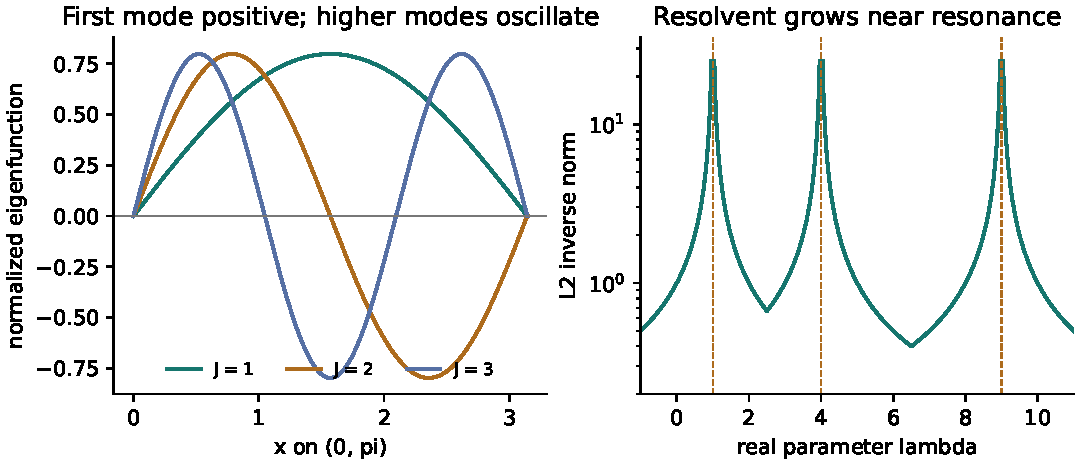
\includegraphics[width=\linewidth]{output/figures/ch06-modes-resonance.pdf}
\end{center}
{\small\textit{Explicit interval model.} On $(0,\pi)$ the Dirichlet
eigenvalues are $j^2$. For real $\lambda$ off the spectrum, the
self-adjoint inverse norm is
$\|(-\partial_{xx}-\lambda)^{-1}\|_{L^2\to L^2}
=1/\min_j|j^2-\lambda|$. The poles mark loss of uniqueness.}
\end{minipage}

\paragraph{Weyl's law: a source remark, not a proved theorem here.}
For the Dirichlet Laplacian on a smooth bounded domain,
\[
 N(\lambda):=\#\{j:\lambda_j\leq\lambda\}
 \sim \frac{\omega_n|U|}{(2\pi)^n}\lambda^{n/2}.
\]
Equivalently,
$\lambda_j\sim4\pi^2(j/(\omega_n|U|))^{2/n}$.
This asymptotic statement appears as a remark in Evans; its proof
requires additional spectral estimates and is not part of the
compactness argument above. Here $\omega_n$ is the volume of the unit ball.

\input{chapters/06-second-order-elliptic-equations/05-nonsymmetric-spectrum}
% Evans 6.6: English printed pp.343--348 / PDF pp.360--365.
\Needspace{65mm}
\section{Problems and Worked Solutions}
\label{sec:6-6}
These are concise restatements of the 17 source problems, with editorial
solutions. Unless a problem says otherwise, $U$ is bounded with smooth
boundary, coefficients are smooth and bounded, and ellipticity is uniform.
Connectedness is specified where constants or positivity are involved.
The same assumptions apply to each weak formulation below.

\Needspace{30mm}
\paragraph{1. Removing a potential by a positive solution.}
Relate $-\Delta u+cu=0$ to $-\operatorname{div}(aDv)=0$.
\begin{proof}[Solution]
If $w>0$ solves the first equation, set $u=wv$. The product rule gives
\[
 -\Delta(wv)+cwv
 =-w\Delta v-2Dw\cdot Dv+v(-\Delta w+cw)
 =-w^{-1}\operatorname{div}(w^2Dv).
\]
Thus $u$ solves the first equation exactly when $v=u/w$ solves the
second with $a=w^2$.
Conversely, given a smooth positive $a$, set $w=\sqrt a$ and
$c=\Delta w/w$. Then $-\Delta w+cw=0$, so the same identity proves
that $u=\sqrt a\,v$ solves the potential equation.
These are local identities wherever $w>0$; uniform bounds on $a$
are additional requirements for a uniform elliptic theory.
\end{proof}
\Needspace{45mm}
\PDEAnnotation{正解作为新的权重}{除以一个正解后，零阶项被吸收到权重 $w^2$ 中。关键是展开 $-\Delta(wv)$ 时保留两倍交叉项；反向构造的势是 $\Delta\sqrt a/\sqrt a$。}

\Needspace{30mm}

\Needspace{45mm}
\PDEAnnotation{负势可以由梯度能量吸收}{零阶系数略微为负并不立即破坏可解性。Poincar\'e 不等式把函数平方项转回梯度项；负势大小的阈值因此与区域几何有关。}
\paragraph{2. A small negative potential.}
For $L=-\partial_j(a^{ij}\partial_i)+c$, find $\mu>0$ so that
$c\geq-\mu$ ensures Lax--Milgram.
\begin{proof}[Solution]
Let $\|u\|_2\leq C_P\|Du\|_2$ on $H^1_0(U)$ and choose
$\mu=\theta/(2C_P^2)$. Then
\[
 B[u,u]\geq\theta\|Du\|_2^2-\mu\|u\|_2^2
 \geq\tfrac{\theta}{2}\|Du\|_2^2\geq C\|u\|_{H^1}^2.
\]
Bounded coefficients give boundedness of $B$. Apply
Theorem~\ref{thm:6-lax-milgram}. The permitted negative part depends on
both ellipticity and the domain's Poincar\'e constant.
\end{proof}

\Needspace{30mm}
\paragraph{3. The clamped biharmonic problem.}
For $f\in L^2(U)$, solve
$\Delta^2u=f$, with $u=\partial_\nu u=0$, weakly in $H^2_0(U)$.
\begin{proof}[Solution]
Use $B_2[u,v]=\int\Delta u\,\Delta v$ and $\ell(v)=\int fv$.
For $u\in C^\infty_c(U)$, integration by parts twice gives
\[
 \int(\Delta u)^2=\sum_{i,j}\int u_{ii}u_{jj}
                  =\sum_{i,j}\int u_{ij}^2.
\]
Approximation extends this to $H^2_0(U)$.
Since $u$ and each $u_i$ belong to $H^1_0(U)$, Poincar\'e applied twice
gives $\|u\|_{H^2}\leq C\|D^2u\|_2$.
Thus $B_2$ is bounded and coercive on $H^2_0$ and $\ell$ is bounded.
Lax--Milgram gives exactly one weak solution. On smooth boundaries
the closure definition of $H^2_0$ encodes both zero traces.
\end{proof}
\Needspace{45mm}
\PDEAnnotation{四阶方程用二阶能量空间}{双调和方程分部积分两次后只需二阶弱导数。$H^2_0$ 同时编码函数及一阶迹为零，不能用只有函数零迹的 $H^2\cap H^1_0$ 随意替代。}

\Needspace{30mm}
\paragraph{4. Neumann compatibility.}
For connected $U$, prove that
$\int Du\cdot Dv=\int fv$ for every $v\in H^1(U)$ is solvable exactly
when $\int_U f=0$.
\begin{proof}[Solution]
Testing with $v=1$ proves necessity. On
$V=\{u\in H^1(U):\int_Uu=0\}$, the mean-zero Poincar\'e inequality holds.
To see this, a counterexample can be normalized to have $\|u_j\|_2=1$,
mean zero and $\|Du_j\|_2\to0$.
Rellich gives a strong $L^2$ limit, whose weak gradient is zero.
It is constant by connectedness and zero by its mean, contradicting norm one.
Lax--Milgram on $V$ gives a unique mean-zero solution.
For arbitrary $v$, subtract its mean; the removed constant contributes
zero on both sides because $\int f=0$. Thus the full weak equation holds.
The difference of any two solutions has zero gradient, so all solutions
differ by a constant.
\end{proof}

\Needspace{30mm}
\paragraph{5. Robin boundary conditions.}
Formulate and solve $-\Delta u=f$, $u+\partial_\nu u=0$.
\begin{proof}[Solution]
Use $H^1(U)$ and its trace $T$, with
\[
 B_R[u,v]=\int_U Du\cdot Dv+\int_{\partial U}Tu\,Tv,\qquad
 \ell(v)=\int_Ufv.
\]
The plus boundary term follows from $\partial_\nu u=-u$ in Green's formula.
Trace boundedness makes $B_R$ bounded. Also
\[
 \|u\|_{H^1}^2\leq C\left(\|Du\|_2^2+
                            \|Tu\|_{L^2(\partial U)}^2\right).
\]
Otherwise normalize a violating sequence to norm one. Its gradients
and traces tend to zero; Rellich and weak $H^1$ convergence yield a
constant on each component, with zero trace, hence zero.
Strong $L^2$ convergence and vanishing gradients contradict norm one.
This proves coercivity; Lax--Milgram yields a unique solution for every $f$.
\end{proof}
\Needspace{45mm}
\PDEAnnotation{边界项也能控制常数}{Neumann 能量看不见常数，所以需要相容条件并允许加常数。Robin 能量多了边界平方项，常数方向也受到控制，于是无需零均值条件且解唯一。}

\Needspace{30mm}

\Needspace{45mm}
\PDEAnnotation{自然边界与本质边界}{Dirichlet 条件先限制解和测试函数所在空间，称为本质条件；Neumann 条件由分部积分后的边界项体现，称为自然条件。更换边界类型也就更换了变分空间。}
\paragraph{6. Mixed Dirichlet--Neumann data.}
Let connected $U$ have $\partial U=\Gamma_1\cup\Gamma_2$ with disjoint
closed pieces. Impose $u=0$ on $\Gamma_1$ and $\partial_\nu u=0$ on $\Gamma_2$.
\begin{proof}[Solution]
Set $V=\{u\in H^1(U):Tu=0\text{ on }\Gamma_1\}$ and require
$\int Du\cdot Dv=\int fv$ for every $v\in V$.
The Dirichlet condition is built into $V$; the Neumann condition appears
naturally after integration by parts.
If $\Gamma_1$ has positive surface measure, Poincar\'e holds on $V$:
a normalized counterexample converges to a constant by the argument
in Problem 4, and its zero trace on $\Gamma_1$ forces that constant to vanish.
Lax--Milgram gives existence and uniqueness for every $f$.
Under the stated smoothness and disjoint closed partition, a nonempty
$\Gamma_1$ is relatively open in $\partial U$ and has positive measure.
If $\Gamma_1$ is empty, Problem 4 gives the Neumann compatibility and
constant ambiguity. If $\Gamma_2$ is empty, this is the usual Dirichlet problem.
For more general partitions that meet along an interface, the weak
formulation still makes sense, but global $H^2$ regularity is a separate issue.
\end{proof}

\Needspace{30mm}
\paragraph{7. A monotone semilinear estimate.}
Let $u\in H^1(\R^n)$ have compact support and solve
$-\Delta u+c(u)=f$ weakly, where $c$ is smooth, $c(0)=0$, $c'\geq0$,
and $c(u),f\in L^2(\R^n)$. Prove $\|D^2u\|_2\leq C\|f\|_2$.
\begin{proof}[Solution]
For fixed $h$ in direction $e_k$, use
$v=-\delta_{-h}\delta_hu\in H^1(\R^n)$, an admissible compactly
supported weak test by density.
Discrete integration by parts gives
\[
 \|\delta_hDu\|_2^2+
 \int_{\R^n}\delta_h(c(u))\,\delta_hu
 =-\int_{\R^n}f\,\delta_{-h}\delta_hu.
\]
The second term is nonnegative because
$(c(s)-c(t))(s-t)\geq0$. Moreover,
$\|\delta_{-h}\delta_hu\|_2\leq\|\partial_k\delta_hu\|_2
\leq\|\delta_hDu\|_2$.
Hence $\|\delta_hDu\|_2\leq\|f\|_2$ uniformly in $h$.
The difference quotient criterion in each direction yields $u\in H^2$ and,
for the Frobenius norm, $\|D^2u\|_2\leq\sqrt n\,\|f\|_2$.
No upper bound on $c'$ is required in this monotonicity argument.
\end{proof}
\Needspace{45mm}
\PDEAnnotation{单调性替代导数上界}{非线性项的差商乘积非负，因此可以留在左边后直接舍去。这里使用的是 $c$ 的单调性，不需要把 $c'(u)$ 当作有界系数来估计。}

\Needspace{30mm}
\paragraph{8. Bernstein's gradient estimate.}
For $Lu=-a^{ij}u_{ij}=0$, show that
$v=|Du|^2+Mu^2$ is a subsolution for large $M$ and deduce a boundary estimate.
\begin{proof}[Solution]
Differentiate the equation to get
$Lu_k=(\partial_k a^{ij})u_{ij}$. Thus
\[
 L|Du|^2
 =-2a^{ij}u_{ki}u_{kj}
       +2u_k(\partial_k a^{ij})u_{ij}
 \leq-\theta|D^2u|^2+C|Du|^2 .
\]
Also $L(u^2)=-2a^{ij}u_i u_j\leq-2\theta|Du|^2$.
Choose $2M\theta\geq C$. Then $Lv\leq0$.
The weak maximum principle gives
$\sup_U|Du|^2\leq\sup_{\partial U}(|Du|^2+Mu^2)$, hence
\[
 \|Du\|_{L^\infty(U)}
 \leq C\bigl(\|Du\|_{L^\infty(\partial U)}
               +\|u\|_{L^\infty(\partial U)}\bigr).
\]
\end{proof}

\Needspace{30mm}
\paragraph{9. A boundary barrier estimate.}
For $Lu=-a^{ij}u_{ij}=f$, $u=0$ on $\partial U$, suppose
$Lw\geq1$, $w\geq0$ on $\partial U$, and $w(x_0)=0$.
\begin{proof}[Solution]
The minimum principle gives $w\geq0$ in $U$.
Let $F=\|f\|_\infty$. Since
$L(\pm u-Fw)\leq0$ and $\pm u-Fw\leq0$ on the boundary,
comparison gives $|u|\leq Fw$.
Assuming the indicated boundary derivatives exist, evaluate at
$x_0-t\nu$ and divide by $t$ to obtain
$|\partial_\nu u(x_0)|\leq F|\partial_\nu w(x_0)|$.
All tangential derivatives of the smooth zero-boundary function $u$
vanish at $x_0$, so $|Du(x_0)|=|\partial_\nu u(x_0)|$.
This is the desired estimate, with constant $F$.
\end{proof}
\Needspace{45mm}
\PDEAnnotation{屏障把函数值变成法向斜率}{先比较得到整个区域的 $|u|\leq\|f\|_\infty w$，再沿内法线取差商。边界上 $u$ 恒为零，所以梯度只剩法向分量。}

\Needspace{30mm}

\Needspace{80mm}
\PDEAnnotation{同一唯一性可有两种证明}{能量法用积分把整个梯度消掉；最大值原理通过极值位置与边界斜率制造矛盾。前者更适合弱解，后者直接揭示正性与边界几何的作用。}
\paragraph{10. Harmonic Neumann solutions are constant.}
Give energy and maximum-principle proofs on connected $U$.
\begin{proof}[Solution]
Green's identity gives
$\int_U|Du|^2=-\int_Uu\Delta u+\int_{\partial U}u\partial_\nu u=0$,
so $Du=0$ and connectedness gives constancy.
Alternatively, if $u$ were nonconstant, its maximum would be on the
boundary by the strong maximum principle and all interior values would
be strictly smaller. Hopf's lemma at a boundary maximum would imply
$\partial_\nu u>0$, contradicting the homogeneous Neumann condition.
The latter proof uses a smooth boundary, or at least the needed interior ball.
\end{proof}

\Needspace{30mm}
\paragraph{11. Convex functions of weak solutions.}
If bounded $u\in H^1(U)$ satisfies
$\int A Du\cdot Dv=0$ for $v\in H^1_0(U)$, prove that
$w=\varphi(u)$ is a weak subsolution for smooth convex $\varphi$.
\begin{proof}[Solution]
The bounded range of $u$ makes $\varphi',\varphi''$ bounded on that range,
so $w\in H^1(U)$ and $Dw=\varphi'(u)Du$.
First take bounded $0\leq v\in H^1_0(U)$.
The product $\varphi'(u)v\in H^1_0(U)$ is an admissible test and gives
\[
 \int A Dw\cdot Dv
 =-\int \varphi''(u)v\, A Du\cdot Du\leq0 .
\]
For arbitrary $0\leq v\in H^1_0(U)$, use
$v_M=\min(v,M)$ and pass in the left side by $v_M\to v$ in $H^1$.
This proves the required inequality for every nonnegative weak test.
The function $w$ need not have zero trace.
\end{proof}
\Needspace{45mm}
\PDEAnnotation{测试函数的乘积要先检查}{若 $v$ 无界，$\varphi''(u)vDu$ 未必属于 $L^2$，不能直接宣布 $\varphi'(u)v$ 合法。先截断 $v$，证明不等式后再用 $H^1$ 收敛去掉截断。}

\Needspace{30mm}
\paragraph{12. A positive supersolution implies comparison.}
Assume $h\in C^2(U)\cap C(\overline U)$,
$h>0$ on \emph{all of} $\overline U$, and $Lh\geq0$.
Prove the zero-boundary weak maximum principle without assuming $c\geq0$.
\begin{proof}[Solution]
For $Lu\leq0$ and $u\leq0$ on $\partial U$, set $z=u/h$.
The product formula gives
\[
 Lu=hMz+zLh,\qquad
 M=-A:D^2+(b-2ADh/h)\cdot D.
\]
On $\{z>0\}$, $Mz\leq0$ and $M$ has no potential.
For each $\varepsilon>0$, the closure of $\{z>\varepsilon\}$ is compact
in $U$, because $z\leq0$ on the boundary and $\min_{\overline U}h>0$.
The drift is bounded there, so the zero-potential maximum principle
gives $z\leq\varepsilon$ on this set, which must therefore be empty.
Let $\varepsilon\downarrow0$.
Positivity only in $U$ would not suffice:
$h=\sin x$ for $L=-\partial_{xx}-1$ on $(0,\pi)$ is an interior
positive solution but vanishes at the endpoints, and comparison fails.
\end{proof}

\Needspace{30mm}
\paragraph{13. Courant's max--min principle.}
For the symmetric operator of \S\ref{sec:6-5}, show
\[
 \lambda_k=\max_{\dim S=k-1}\ \min_{\substack{u\in H^1_0(U)\cap S^\perp\\\|u\|_2=1}} B[u,u],
\]
where $S\subset H^1_0(U)$ and orthogonality is in $L^2(U)$.
\begin{proof}[Solution]
For any such $S$, linear algebra supplies a nonzero vector in
$\operatorname{span}(w_1,\ldots,w_k)\cap S^\perp$.
Normalize it. Formula~\eqref{eq:6-energy-spectrum} gives its energy
at most $\lambda_k$, so the inner minimum is at most $\lambda_k$.
For $S=\operatorname{span}(w_1,\ldots,w_{k-1})$, every admissible $u$
has only modes $j\geq k$, and the same formula gives
$B[u,u]\geq\lambda_k$. Equality occurs at $w_k$.
For any fixed $S$, the minimum exists by the direct method; its
orthogonality constraints are preserved by strong $L^2$ convergence.
\end{proof}
\Needspace{45mm}
\PDEAnnotation{极小极大中的正交空间}{这里去掉的是前若干模态在 $L^2$ 中的方向。任意少于 $k$ 个线性约束都不可能消灭前 $k$ 个模态的全部组合，这就是一半不等式的有限维理由。}

\Needspace{30mm}

\Needspace{45mm}
\PDEAnnotation{非对称公式中的权重来自伴随}{不能只对 $Lu/u$ 做普通空间平均。与正的伴随特征函数配对后，正确权重是 $u\phi^*$；分部积分才把这个加权平均固定为主特征值。}
\paragraph{14. A principal-eigenvalue max--min formula.}
For the nonsymmetric operator, prove
\[
 \lambda_1=\sup_{\substack{u\in C^\infty(\overline U),\
                  u>0\text{ in }U\\u=0\text{ on }\partial U}}
                  \ \inf_{x\in U}\frac{Lu(x)}{u(x)}.
\]
\begin{proof}[Solution]
Let $\phi^*>0$ be the adjoint eigenfunction from
Lemma~\ref{lem:6-positive-adjoint}. Both functions have zero trace,
so Green's identity, or the weak adjoint identity, gives
\[
 \int_U\phi^*Lu=\int_UuL^*\phi^*
                =\lambda_1\int_Uu\phi^*.
\]
Thus the weighted average of $Lu/u$ with positive weight $u\phi^*$
is $\lambda_1$. Its infimum cannot exceed this average.
If the infimum is $-\infty$ the inequality is immediate; otherwise
integrating its pointwise lower bound proves it directly.
Taking $u=\phi$ achieves equality everywhere.
A constant shift handles potentials of arbitrary bounded sign.
\end{proof}

\Needspace{30mm}
\paragraph{15. Hadamard's domain-variation formula.}
Let $-\Delta w=\lambda w$ on a smoothly moving domain $U(\tau)$,
$w=0$ on its boundary and $\int_{U(\tau)}w^2=1$.
Assume a smooth eigenvalue/eigenfunction branch, and denote boundary
velocity by $\mathbf v$.
\begin{proof}[Solution]
Use the Eulerian derivative $\dot w$ at a fixed spatial point.
Differentiating $w(x(\tau),\tau)=0$ on the moving boundary gives
\[
 \dot w=-Dw\cdot\mathbf v
       =-\partial_\nu w\,(\mathbf v\cdot\nu).
\]
Reynolds' formula for normalization yields
$2\int_Uw\dot w+\int_{\partial U}w^2\mathbf v\cdot\nu=0$,
hence $\int_Uw\dot w=0$.
Since $\lambda=\int_U|Dw|^2$, differentiate once more:
\begin{align*}
 \dot\lambda
 &=2\int_U Dw\cdot D\dot w+
             \int_{\partial U}|Dw|^2\mathbf v\cdot\nu\\
 &=2\lambda\int_Uw\dot w+
      2\int_{\partial U}\partial_\nu w\,\dot w+
             \int_{\partial U}(\partial_\nu w)^2\mathbf v\cdot\nu\\
 &=-\int_{\partial U}(\partial_\nu w)^2\mathbf v\cdot\nu.
\end{align*}
Tangential derivatives vanish because $w$ is zero on the boundary.
The smooth-branch hypothesis is essential; a multiple eigenvalue need
not admit a single arbitrarily chosen differentiable eigenfunction branch.
\end{proof}
\Needspace{45mm}
\PDEAnnotation{扩张区域使特征值下降}{若边界向外移动，$\mathbf v\cdot\nu>0$，公式给出 $\dot\lambda<0$。负号来自移动边界条件 $\dot w=-\partial_\nu w\,\mathbf v\cdot\nu$，不是凭直觉添加。}

\Needspace{30mm}

\Needspace{45mm}
\PDEAnnotation{辐射条件选择向外传播}{时间因子取 $e^{-i\sigma t}$ 时，$e^{i\sigma r}/r$ 描述向外传播的球面波。条件中的减号与这一时间约定配套；平面波不会在所有方向都向外辐射。}
\paragraph{16. Helmholtz waves and radiation.}
Let real $\sigma\ne0$ and $\lambda=\sigma^2$.
\begin{proof}[Solution]
(a) For $|\omega|=1$,
$-\Delta e^{i\sigma\omega\cdot x}=\sigma^2e^{i\sigma\omega\cdot x}$.
Thus $e^{i\sigma(\omega\cdot x-t)}$ solves the wave equation.

(b) In dimension three put
$\Phi(x)=e^{i\sigma r}/(4\pi r)$, $r=|x|$.
The radial identity $\Delta g=g''+2g'/r$ shows
$(-\Delta-\sigma^2)\Phi=0$ for $r>0$.
At $r=\varepsilon$,
\[
 -\int_{\partial B_\varepsilon}\partial_r\Phi\,dS
 =e^{i\sigma\varepsilon}(1-i\sigma\varepsilon)\longrightarrow1.
\]
Integration by parts against a smooth test function outside
$B_\varepsilon$ therefore gives
$(-\Delta-\sigma^2)\Phi=\delta_0$; the other shrinking-sphere term and
the volume integral of $\sigma^2\Phi$ tend to zero.

(c) For $\Phi$,
$r(\Phi_r-i\sigma\Phi)=-e^{i\sigma r}/(4\pi r)\to0$ uniformly in angle.
For the plane wave at $x=r\vartheta$,
\[
 r(w_r-i\sigma w)
 =i\sigma r(\omega\cdot\vartheta-1)e^{i\sigma r\omega\cdot\vartheta},
\]
whose modulus diverges on every ray with $\omega\cdot\vartheta\ne1$.
Thus the plane wave does not satisfy the Sommerfeld condition.
\end{proof}

\Needspace{30mm}
\paragraph{17. Uniqueness of an entire radiating solution.}
Suppose $w$ solves $-\Delta w=\sigma^2w$ throughout $\R^3$ and satisfies
$r(w_r-i\sigma w)\to0$ \emph{uniformly in angle}. Prove $w=0$.
\begin{proof}[Solution]
Green's identity and the real coefficient $\sigma^2$ imply
\[
 0=\int_{\partial B_R}(\overline w\,w_r-w\,\overline{w_r})\,dS.
\]
The imaginary flux is zero, so expansion of the square gives
\[
 \int_{\partial B_R}(|w_r|^2+\sigma^2|w|^2)\,dS
 =\int_{\partial B_R}|w_r-i\sigma w|^2\,dS=o(1).
\]
Uniform radiation justifies the last step, since the sphere has area
$4\pi R^2$ and the integrand is $o(R^{-2})$ uniformly.
For a fixed $x_0$ and $R>|x_0|$, Green's representation with the
outgoing kernel $\Phi(x-x_0)$ gives
\[
 w(x_0)=\int_{\partial B_R}
   \bigl(\Phi\,w_r-w\,\partial_r\Phi\bigr)\,dS .
\]
Here $\partial_r$ on the kernel means the outward derivative on
$\partial B_R$, not radial differentiation about $x_0$.
For large $R$, both $\Phi(x-x_0)$ and this derivative are $O(R^{-1})$,
so their $L^2(\partial B_R)$ norms remain bounded.
Cauchy--Schwarz and the vanishing flux norm above imply $w(x_0)=0$.
Since $x_0$ was arbitrary, $w\equiv0$.
\end{proof}
\Needspace{45mm}
\PDEAnnotation{辐射条件还包含一致性}{从逐方向极限跳到球面积分极限需要控制角变量。这里明确采用对方向一致的 Sommerfeld 条件；基本解在原点有奇性，所以并不违背“全空间光滑辐射解只能为零”。}

% Evans 6.7: English printed p.348 / PDF p.365; Chinese printed p.246 / PDF p.264.
\Needspace{65mm}
\section{References and Proof Dependencies}
\label{sec:6-7}
The primary source is Lawrence C. Evans, \emph{Partial Differential
Equations}, second edition, Chapter~6, printed pp.~293--348
(local English PDF pp.~310--365). The Chinese scan corresponds to
printed pp.~208--246 (PDF pp.~226--264); selected page comparisons
are recorded in \texttt{docs/CHAPTER-06.md}.
The English prose, proof expansions, solutions and Chinese annotations
here are editorial reconstructions.

Evans's references point to Gilbarg--Trudinger for weak elliptic theory,
regularity, maximum principles and Harnack; Krylov and
Ladyzhenskaya--Uraltseva for regularity; Protter--Weinberger and
Pucci--Serrin for maximum principles; and Smoller for spectral theory.
For domain variations the source cites Garabedian; for radiation it
cites Colton. These are source bibliography pointers, not claims
that those books have been independently consulted for this draft.

\paragraph{Dependencies and boundaries.}
Riesz representation, Hilbert weak compactness and Hilbert Parseval
are prerequisites. Chapter~5 supplies the Sobolev tools.
Lax--Milgram, the compact Fredholm lemma, regularity, maximum principles,
the smooth principal-part Harnack inequality, compact self-adjoint
spectral decomposition and the principal-eigenvalue arguments are
expanded above. The nonsymmetric existence proof explicitly invokes
Schaefer's fixed-point theorem. Weyl's law is stated as an unproved
source remark. The general measurable-coefficient Harnack theorem
is described as an extension, not claimed as proved.
All 17 source problems have editorial solutions.
Compilation, model calculations and layout checks do not constitute
independent mathematical review; this chapter remains an author-checked
study draft.
% Source: English Chapter 7, printed p. 349, PDF page 366.
\chapter{Linear Evolution Equations}
\label{chap:linear-evolution-equations}

\PDESource
  {Chapter 7; printed p.~349; PDF page~366}
  {中译本对应章：线性发展方程，书内第 248 页起。}

\noindent\textbf{Status: outline only / 目录骨架。}
English exposition, Chinese margin notes, and expanded proofs will be added section by section.

% Evans second edition, section 7.1.
% English source: printed p. 349; PDF page 366 (1-based).
% Chinese subsection/page correspondence: pending verification against the scan.
% Status: outline-only; no source text or proof has been transcribed/reviewed.
\section{Second-Order Parabolic Equations}
\label{sec:7-1}

\PDEPending

% TODO: English exposition with source theorem/equation identifiers.
% TODO: Add necessary \PDEVocab, \PDEIdea, or \PDEChinese notes.
% TODO: Expand abbreviated arguments in expandedproof/proofdetails.
% TODO: Verify hypotheses, endpoints, constants, limits, and cross-references.

% Evans 7.2: printed pp.375--396 / English PDF pp.392--413.
% Chinese: printed pp.266--279 / scan pp.284--297.
\Needspace{55mm}
\section{Second-Order Hyperbolic Equations}
\label{sec:7-2}
\Needspace{55mm}
\subsection{Two initial data and the natural energy}
Keep $V=H^1_0(U)$, $H=L^2(U)$ and the divergence-form $L(t)$ from
\S\ref{sec:7-1}. Here assume $a^{ij},b^i,c\in C^1(\overline Q_T)$,
$a^{ij}=a^{ji}$, with the same uniform ellipticity bound. Study
\begin{equation}\label{eq:7-wave}
 u''+L(t)u=f,\quad u|_{\partial U}=0,\quad u(0)=g,\ u'(0)=h,
\end{equation}
where $g\in V$, $h\in H$, $f\in L^2(0,T;H)$.
A weak solution has
\[
 u\in L^2V,\quad u'\in L^2H,\quad u''\in L^2V',\qquad
 \langle u'',v\rangle+B_t[u,v]=(f,v).
\]
The initial values are meaningful in $H$ and $V'$, respectively:
$u\in H^1(0,T;H)\subset C([0,T];H)$ and
$u'\in H^1(0,T;V')\subset C([0,T];V')$.
The estimates below in fact put $u,u'$ in $L^\infty V,L^\infty H$.
\Needspace{55mm}
\PDEAnnotation{位移和速度的不同空间}{能量包含 $\|Du\|_2^2+\|u_t\|_2^2$，故自然数据为 $g\in H^1_0$、$h\in L^2$。基本弱解定义中速度初值先在 $H^{-1}$ 识别，不能无证明地宣称 $u_t$ 在 $L^2$ 连续。}

\Needspace{55mm}
\begin{theorem}[Energy bound and existence; source \S7.2.2, Theorems 1--3]
\label{thm:7-wave-existence}
There exists a weak solution satisfying
\begin{equation}\label{eq:7-wave-energy}
 \begin{split}
 &\mathop{\rm ess\,sup}_{0<t<T}
 (\|u(t)\|_V^2+\|u'(t)\|_H^2)+\|u''\|_{L^2V'}^2\\
 &\hspace{15mm}\leq C(\|g\|_V^2+\|h\|_H^2+\|f\|_{L^2H}^2).
 \end{split}
\end{equation}
\end{theorem}
\begin{expandedproof}[the second-order finite system]
Use the same $V_m$ and solve
\[
 (u_m'',w_k)+B_t[u_m,w_k]=(f,w_k),\quad
 u_m(0)=P_mg,\quad u_m'(0)=P_mh.
\]
This finite second-order system becomes a linear first-order ODE in
$(d,d')$, so has a unique solution. Test with $u_m'$ and put
\[
 E_m=\tfrac12\big(\|u_m'\|_H^2+
          \int_Ua^{ij}(u_m)_i(u_m)_j+\|u_m\|_H^2\big).
\]
A direct calculation gives
\[
 E_m'=(f,u_m')-\int_U(b^i(u_m)_i+cu_m)u_m'
      +\tfrac12\int_Ua_t^{ij}(u_m)_i(u_m)_j+(u_m,u_m').
\]
Thus $E_m'\leq CE_m+C\|f\|_H^2$. Gronwall gives the uniform energy
bound; $E_m$ is equivalent to $\|u_m\|_V^2+\|u_m'\|_H^2$.
Using $P_m$ in an arbitrary test gives
$\|u_m''\|_{V'}\leq C\|u_m\|_V+C\|f\|_H$.
Weak compactness yields the equation and identifies successive weak
derivatives by scalar time tests, exactly as in the parabolic construction.

For $v\in V_N$, $m\geq N$, and $\phi(T)=\phi'(T)=0$, twice integrating
in time gives
\[
 \begin{split}
 \int_0^T\{(u_m,v)\phi''+B_t[u_m,v]\phi\}\,dt
 ={}&\int_0^T(f,v)\phi\,dt\\
 &+(P_mh,v)\phi(0)-(P_mg,v)\phi'(0).
 \end{split}
\]
Both endpoint coefficients survive the weak limit. Comparing with the
trace formula for $u,u'$ identifies $u(0)=g$, $u'(0)=h$. Lower
semicontinuity, including the time-set argument of Problem 6, gives
\eqref{eq:7-wave-energy}.
\end{expandedproof}

\Needspace{55mm}
\subsection{Uniqueness without testing by an unavailable derivative}
A weak solution need not have $u'\in V$, so the formal test $v=u'$ is
not legitimate. The source's integrated test repairs this gap.
\Needspace{55mm}
\begin{theorem}[Weak uniqueness; source Theorem 4]
\label{thm:7-wave-unique}
The weak solution of \eqref{eq:7-wave} is unique in the class just defined.
\end{theorem}
\begin{expandedproof}[the integrated test]
Subtract two solutions, so $f=g=h=0$. Fix $s$ and use
$v(t)=\int_t^s u(r)\,dr$ for $0\leq t\leq s$. Then $v'=-u$ in $V$,
$v(s)=0$, and $v$ is a legal time-dependent $V$ test by approximation
with finite sums of scalar time tests.
Write $B_t=S_t+K_t$, with $S_t$ symmetric and $K_t$ skew-symmetric.
Integration by parts in space gives
\[
 \begin{split}
 S_t[z,z]&=\int_U a^{ij}z_i z_j+(c-\tfrac12\operatorname{div}b)z^2,\\
 K_t[u,v]&=-\int_Uu\,b\cdot Dv-\tfrac12(\operatorname{div}b)uv.
 \end{split}
\]
In particular $|K_t[u,v]|\leq C\|u\|_H\|v\|_V$,
$|\dot S_t[v,v]|\leq C\|v\|_V^2$ (one may use the original symmetric
formula, avoiding mixed coefficient derivatives).
Also $S_t[v,v]\geq\alpha\|v\|_V^2-\gamma\|v\|_H^2$.
Time integration by parts, with $u'(0)=0$ in $V'$, gives
\[
 \tfrac12\|u(s)\|_H^2+\tfrac12 S_0[v(0),v(0)]
 =-\int_0^s\big(\tfrac12\dot S_t[v,v]+K_t[u,v]\big)\,dt.
\]
Here $\int(u',u)=\frac12\|u(s)\|_H^2$ is valid since $u\in H^1(0,T;H)$;
all other pairings involve $V',V$.
Thus
\[
 \|u(s)\|_H^2+\alpha\|v(0)\|_V^2
 \leq C\int_0^s(\|u\|_H^2+\|v\|_V^2)\,dt+\gamma\|v(0)\|_H^2.
\]
Put $W(t)=\int_0^t u$, so $v(t)=W(s)-W(t)$.
The last term is bounded by $\gamma s\int_0^s\|u\|_H^2$.
Consequently, for a fixed sufficiently short interval,
\[
 \|u(s)\|_H^2+\tfrac\alpha2\|W(s)\|_V^2
 \leq C\int_0^s(\|u(t)\|_H^2+\|W(t)\|_V^2)\,dt.
\]
Gronwall forces $u=0$ there. Restart at its right endpoint: the $H$ and
$V'$ traces are zero, and all constants are uniform on $[0,T]$.
Finitely many repetitions give $u=0$ throughout.
\end{expandedproof}
\Needspace{55mm}
\PDEAnnotation{积分测试恢复合法性}{$v(t)=\int_t^s u$ 属于 $H^1_0$，而 $v'=-u$。它将不可用的 $u_t$ 测试转成合法的时间分部积分；短时间吸收后再拼接，覆盖整个时间区间。}

\Needspace{55mm}
\subsection{Higher regularity and the absence of smoothing}
For the remainder of the bounded-domain regularity discussion, coefficients
are smooth and time independent.
\Needspace{55mm}
\begin{theorem}[Improved wave regularity; source \S7.2.3, Theorem 5]
If $g\in H^2(U)\cap V$, $h\in V$, and $f\in H^1(0,T;H)$, then
\[
 u\in L^\infty H^2,\quad u'\in L^\infty V,\quad
 u''\in L^\infty H,\quad u'''\in L^2V',
\]
with norm bound $C(\|g\|_{H^2}+\|h\|_V+\|f\|_{H^1(0,T;H)})$.
\end{theorem}
\begin{expandedproof}[reconstruction instead of formal differentiation]
Construct $v$ solving $v''+Lv=f'$ with initial data
$v(0)=h$, $v'(0)=f(0)-Lg\in H$. Set $U=g+\int_0^t v$.
In distributions,
$(U''+LU-f)'=v''+Lv-f'=0$, while the residual at $0$ is zero in $V'$.
Hence $U$ solves the original equation and has data $g,h$.
Uniqueness gives $U=u$, $u'=v$. Estimate $v$ by
\eqref{eq:7-wave-energy} and recover $u\in L^\infty H^2$ from
$Lu=f-u''$ and the elliptic estimate. This proves every stated norm bound.
\end{expandedproof}
\Needspace{55mm}
\begin{theorem}[Higher wave regularity; source Theorems 6--7]
Let $m\geq0$, $g\in H^{m+1}(U)$, $h\in H^m(U)$, and
$\partial_t^kf\in L^2H^{m-k}(U)$ for $0\leq k\leq m$.
Set $q_0=g$, $q_1=h$, and
\[
 q_{j+2}=\partial_t^j f(0)-Lq_j\quad(0\leq j\leq m-2).
\]
Require $q_j\in V$ for $0\leq j\leq m$ (for $m=0$ only $g\in V$).
Then
\[
 \begin{split}
 &\mathop{\rm ess\,sup}_{0<t<T}\sum_{k=0}^{m+1}
 \|\partial_t^ku(t)\|_{H^{m+1-k}}\\
 &\qquad\leq C\left(\|g\|_{H^{m+1}}+\|h\|_{H^m}
 +\sum_{k=0}^{m}\|\partial_t^kf\|_{L^2H^{m-k}}\right).
 \end{split}
\]
Smooth data compatible to every order give a smooth solution on the closed cylinder.
\end{theorem}
\begin{expandedproof}[one time derivative at each induction step]
The case $m=0$ is the basic wave bound. In passing to $m+1$, the preceding
reconstruction gives $v=u'$ with data $h,f(0)-Lg$ and forcing $f'$.
Its compatibility sequence is shifted by one place. Apply induction to $v$.
The trace inequality
$\|F(0)\|_{H^r}\leq C(\|F\|_{L^2H^r}+\|F'\|_{L^2H^r})$
controls the forcing traces required at this step.
Then $Lu=f-u''$ and elliptic regularity recover the missing highest spatial
norm of $u$. This proves the estimate and the induction. Arbitrarily high
mixed Sobolev regularity and embedding prove the smooth conclusion.
\end{expandedproof}
\Needspace{55mm}
\PDEAnnotation{波动不会自动磨光}{$\sin(kx)$ 模态的位移为 $\cos(kt)\sin(kx)$；高频振幅没有热方程的 $e^{-k^2t}$ 衰减。提高解的正则性需要提高初值正则性，不能从能量估计推导任意正时刻光滑。}

\Needspace{55mm}
\subsection{Finite propagation and the geometry of the cone}
On $\R^n$ now take the source's nondivergence model
$u_{tt}-a^{ij}(x)u_{ij}=0$ with smooth symmetric positive $A$.
Assume on the region under consideration that an optical distance $q$ is
smooth away from $x_0$, positive there, $q(x_0)=0$, and
\[
 A Dq\cdot Dq=1.
\]
Assume its relevant sublevel sets are bounded and shrink to $x_0$.
Set $K_t=\{q<t_0-t\}$ for $0\leq t<t_0$ and
$K=\{(x,t):0\leq t<t_0,\ x\in K_t\}$.
\Needspace{55mm}
\begin{theorem}[Finite propagation; source \S7.2.4, Theorem 8]
If a smooth solution has $u=u_t=0$ on $K_0$, it vanishes throughout $K$,
and at its vertex by continuity.
\end{theorem}
\begin{expandedproof}[coarea, normal speed, and the energy flux]
The outward normal is $\nu=Dq/|Dq|$ and the moving boundary has outward
normal velocity $-1/|Dq|$. Hence for
$E(t)=\frac12\int_{K_t}(u_t^2+A Du\cdot Du)$, differentiation gives
\[
 \begin{split}
 E'(t)={}&-\int_{K_t}u_t(\partial_j a^{ij})u_i
 +\int_{\partial K_t}u_t A Du\cdot\nu\\
 &-\frac12\int_{\partial K_t}
       \frac{u_t^2+A Du\cdot Du}{|Dq|}.
 \end{split}
\]
The volume error is at most $CE(t)$ by ellipticity and bounded first
coefficient derivatives. Also
\[
 |A Du\cdot\nu|\leq(A Du\cdot Du)^{1/2}(A\nu\cdot\nu)^{1/2}
 =\frac{(A Du\cdot Du)^{1/2}}{|Dq|}.
\]
Young's inequality makes the boundary flux no larger than the negative
moving-boundary term. Thus $E'\leq CE$ and $E(0)=0$, giving $E=0$.
For fixed $x\in K_t$, that same $x$ belongs to every earlier $K_s$;
integrating $u_t=0$ from its zero initial value proves $u(x,t)=0$.
\end{expandedproof}
\Needspace{55mm}
\PDEAnnotation{光学距离的局部限制}{度量是 $A^{-1}$，不是 $A$。变系数的距离函数可能有割迹，不能默认全空间光滑；此处光滑 $q$ 是明确假设。常系数时 $q=\sqrt{(x-x_0)^TA^{-1}(x-x_0)}$，波前为椭球。}

\PDEBodyDiagram{7.3}{Anisotropy changes the cross-section of a wave cone.}
{For $A=\operatorname{diag}(4,1)$, $q(x)=\sqrt{x_1^2/4+x_2^2}$. At time $t$, the dependency cross-section is an ellipse with semiaxes $2(t_0-t)$ and $t_0-t$. The cone sketch and the spatial slice use separate coordinate scales.}
{ch07-anisotropic-cone}

\Needspace{55mm}
\subsection{Characteristic coordinates in two variables}
For $a u_{xx}+2b u_{xy}+d u_{yy}+\text{lower terms}=0$, assume smooth
coefficients and $ad-b^2<0$. A coordinate function $\xi$ must solve
\[
 a\xi_x^2+2b\xi_x\xi_y+d\xi_y^2=0.
\]
After a fixed linear coordinate change one can arrange $a\ne0$ near the
point: an indefinite quadratic form cannot vanish on every direction.
Writing $D=b^2-ad>0$ factors this equation into the two distinct fields
\[
 a\xi_x+(b+\sqrt D)\xi_y=0,\qquad
 a\eta_x+(b-\sqrt D)\eta_y=0.
\]
\begin{expandedproof}[local invertibility and both canonical forms]
The two smooth nonzero vector fields are transverse, since their determinant
is $-2a\sqrt D\ne0$. The local flow-box construction (solving the
characteristic ODE from a transverse curve) gives first integrals $\xi,\eta$
with nonzero independent gradients. Thus $\Phi=(\xi,\eta)$ is locally
invertible. By the chain rule the transformed principal matrix is
$\widetilde A=D\Phi\,A\,D\Phi^T$, whose two diagonal entries vanish.
Its determinant is $(\det D\Phi)^2\det A<0$, so the off-diagonal entry
is nonzero. Division yields $v_{\xi\eta}+\text{lower terms}=0$.
For $z_1=\xi+\eta$, $z_2=\xi-\eta$, this becomes
$v_{z_1z_1}-v_{z_2z_2}+\text{lower terms}=0$.
For example $u_{tt}-c^2u_{xx}$, $c>0$, becomes
$-4c^2v_{\xi\eta}$ with $\xi=x-ct$, $\eta=x+ct$.
All these coordinates are local; no global characteristic chart is asserted.
\end{expandedproof}
\Needspace{55mm}
\PDEAnnotation{双曲标准形是局部结论}{判别式给出两个横截特征方向；逆函数定理还需要 $\det D\Phi\ne0$。先处理 $a\ne0$ 的局部坐标，避免在 $a=0$ 处直接除法。}

% Evans second edition, section 7.3.
% English source: printed p. 396; PDF page 413 (1-based).
% Chinese subsection/page correspondence: pending verification against the scan.
% Status: outline-only; no source text or proof has been transcribed/reviewed.
\section{Systems of Hyperbolic First-Order Equations}
\label{sec:7-3}

\PDEPending

% TODO: English exposition with source theorem/equation identifiers.
% TODO: Add necessary \PDEVocab, \PDEIdea, or \PDEChinese notes.
% TODO: Expand abbreviated arguments in expandedproof/proofdetails.
% TODO: Verify hypotheses, endpoints, constants, limits, and cross-references.

% Evans 7.4: printed pp.409--420 / English PDF pp.426--437.
% Chinese: printed pp.289--296 / scan pp.307--314.
\Needspace{55mm}
\section{Semigroup Theory}
\label{sec:7-4}
\Needspace{55mm}
\subsection{Strong continuity, the generator, and its domain}
Let $X$ be a real Banach space. A strongly continuous semigroup is a family
$S(t)\in\mathcal L(X)$, $t\geq0$, satisfying
\[
 S(0)=I,\quad S(t+s)=S(t)S(s),\quad S(t)x\longrightarrow x
 \text{ in }X\text{ as }t\downarrow0.
\]
We first assume $\|S(t)\|\leq1$ (a contraction semigroup).
Its generator is the generally unbounded operator
\[
 D(G)=\left\{x:\lim_{h\downarrow0}\frac{S(h)x-x}{h}
          \text{ exists in }X\right\},\qquad
 Gx=\lim_{h\downarrow0}\frac{S(h)x-x}{h}.
\]
We use $G$ instead of the source's $A$, to distinguish it from the principal
coefficient matrix. For $u_t+Lu=0$, the generator is $G=-L$.
\Needspace{55mm}
\PDEAnnotation{强连续不等于范数连续}{要求每个固定 $x$ 的 $\|S(t)x-x\|\to0$。若要求 $\|S(t)-I\|\to0$，就排除了许多无界生成元，例如 $L^2$ 上的热半群。}

\Needspace{55mm}
\begin{theorem}[Generator properties; source \S7.4.1, Theorems 1--2]
\label{thm:7-generator}
The domain $D(G)$ is dense, and $G$ is closed. For $x\in D(G)$,
$S(t)x\in D(G)$, $GS(t)x=S(t)Gx$, and
\[
 \frac d{dt}S(t)x=GS(t)x=S(t)Gx.
\]
At $t=0$ this is a right derivative. In particular
$S(t)x-x=\int_0^tS(s)Gx\,ds$.
\end{theorem}
\begin{expandedproof}[domain invariance, density, and graph closure]
Commuting $S(t)$ with $S(h)$ and passing to the defining difference quotient
proves invariance and commutation. The right derivative follows likewise;
for the left derivative at $t>0$ use
\[
 \frac{S(t)x-S(t-h)x}{h}=S(t-h)\frac{S(h)x-x}{h}
 \longrightarrow S(t)Gx.
\]
Strong continuity and the contraction bound justify the last limit.
For arbitrary $x\in X$, let $x_t=t^{-1}\int_0^tS(s)x\,ds$.
A change of integration interval gives
\[
 x_t\in D(G),\qquad Gx_t=\frac{S(t)x-x}{t},\qquad x_t\to x.
\]
Thus the domain is dense. To prove closedness, take $x_k\to x$,
$Gx_k\to y$ in $X$ and pass to the limit in
$S(t)x_k-x_k=\int_0^tS(s)Gx_k\,ds$.
The contraction bound makes convergence of the integrals uniform on
bounded time intervals. Divide the limit identity by $t$ and let
$t\downarrow0$: its right side tends to $y$. Hence $x\in D(G)$ and $Gx=y$.
\end{expandedproof}
\Needspace{55mm}
\PDEAnnotation{闭算子与有界算子的区别}{闭性是 $x_k\to x$ 且 $Gx_k\to y$ 时才推出 $Gx=y$，不表示 $\|Gx\|\leq C\|x\|$。热方程的高频特征函数说明后一不等式不成立。}

\Needspace{55mm}
\subsection{Resolvents as Laplace transforms}
For a closed densely defined operator $G$, let $\rho(G)$ be the set of
real $\lambda$ for which $\lambda I-G:D(G)\to X$ is bijective, and
$R_\lambda=(\lambda I-G)^{-1}$. The closed graph theorem makes
$R_\lambda:X\to X$ bounded. Its range is $D(G)$.
\Needspace{55mm}
\begin{theorem}[Resolvent identities and representation; source Theorem 3]
\label{thm:7-resolvent}
For $\lambda,\mu\in\rho(G)$,
\begin{equation}\label{eq:7-resolvent-id}
 R_\lambda-R_\mu=(\mu-\lambda)R_\lambda R_\mu,\qquad
 R_\lambda R_\mu=R_\mu R_\lambda.
\end{equation}
For a contraction generator every $\lambda>0$ is in $\rho(G)$, and
\begin{equation}\label{eq:7-resolvent-laplace}
 R_\lambda x=\int_0^\infty e^{-\lambda t}S(t)x\,dt,
 \qquad\|R_\lambda\|\leq\lambda^{-1}.
\end{equation}
The integral is a norm-convergent Bochner integral.
\end{theorem}
\begin{expandedproof}[the inverse on both sides]
For the first identity insert
$(\mu I-G)-(\lambda I-G)=(\mu-\lambda)I$ between $R_\lambda$ and
$R_\mu$. These compositions are defined because each resolvent maps into
$D(G)$. Interchanging $\lambda,\mu$ gives commutation (equal parameters
are immediate).
Let $J_\lambda x$ denote the integral in \eqref{eq:7-resolvent-laplace}.
It converges since its integrand has norm at most $e^{-\lambda t}\|x\|$.
Changing variables gives
\[
 \frac{S(h)J_\lambda x-J_\lambda x}{h}
 =\frac{e^{\lambda h}-1}{h}J_\lambda x
 -\frac{e^{\lambda h}}h\int_0^he^{-\lambda t}S(t)x\,dt.
\]
The limit is $\lambda J_\lambda x-x$. Thus $J_\lambda x\in D(G)$ and
$(\lambda I-G)J_\lambda x=x$.
For $x\in D(G)$, differentiate $e^{-\lambda t}S(t)x$ and integrate:
\[
 \int_0^\infty e^{-\lambda t}S(t)(\lambda x-Gx)\,dt=x.
\]
The endpoint at infinity vanishes by the contraction bound. Therefore
$J_\lambda$ is also a left inverse, proving bijectivity and the formula.
The norm bound follows by integration. This proof never passes an
unbounded operator through an integral without a domain argument;
Problem 13 gives the equivalent graph-norm justification.
\end{expandedproof}
\Needspace{55mm}
\PDEAnnotation{预解算子的符号}{$G=-L$ 时 $R_\lambda=(\lambda I+L)^{-1}$。椭圆能量估计给出的正参数正好对应发展方程的稳定方向；若误写成 $L-\lambda I$，会引入不应出现的共振。}

\PDEMarginDiagram{7.M}{同一模态的两种衰减}
{热方程取 $E=\frac12\|u\|_2^2$，图示 $k=1$ 模态。波动方程取 $E=\frac12(\|u_t\|_2^2+\|u_x\|_2^2)$，同一模态总能量守恒。}
{ch07-energy-margin}

\Needspace{55mm}
\subsection{Constructing the semigroup from resolvent bounds}
\Needspace{55mm}
\begin{theorem}[Hille--Yosida, contraction case; source \S7.4.2, Theorem 4]
\label{thm:7-hille-yosida}
A closed densely defined linear $G$ generates a contraction semigroup if
and only if
\[
 (0,\infty)\subset\rho(G),\qquad\|R_\lambda\|\leq\lambda^{-1}
 \quad(\lambda>0).
\]
\end{theorem}
\begin{expandedproof}[Yosida approximation]
Necessity is Theorem~\ref{thm:7-resolvent}. Conversely define the bounded
operators
\[
 G_\lambda=\lambda^2R_\lambda-\lambda I=\lambda GR_\lambda.
\]
For $x\in D(G)$,
$\lambda R_\lambda x-x=R_\lambda Gx\to0$.
The bound $\|\lambda R_\lambda\|\leq1$ and density extend this convergence
to every $x\in X$. Consequently $G_\lambda x=\lambda R_\lambda Gx\to Gx$
for $x\in D(G)$.
Put $S_\lambda(t)=e^{tG_\lambda}$. Its power series gives
\[
 \|S_\lambda(t)\|\leq
 e^{-\lambda t}\sum_{k=0}^\infty
       \frac{(\lambda^2t)^k\|R_\lambda\|^k}{k!}\leq1.
\]
The resolvent identity shows that all $G_\lambda$ commute. Differentiate
$S_\mu(t-s)S_\lambda(s)x$ in $s$ and integrate to obtain
\[
 \|S_\lambda(t)x-S_\mu(t)x\|
 \leq t\|(G_\lambda-G_\mu)x\|\longrightarrow0
 \quad(x\in D(G)).
\]
Thus $S_\lambda(t)x$ converges uniformly on bounded time intervals.
Approximation of any $x\in X$ by points of $D(G)$ extends this convergence
to all $X$. The limit $S(t)$ is a contraction, is strongly continuous,
and satisfies the semigroup law: in the product limit use the uniform
operator bound to control one factor and strong convergence for the other.

Let $K$ be its generator. For $x\in D(G)$ pass to the limit in
\[
 S_\lambda(t)x-x=\int_0^tS_\lambda(s)G_\lambda x\,ds
\]
to get $S(t)x-x=\int_0^tS(s)Gx\,ds$. Dividing by $t$ proves
$G\subset K$. This inclusion alone is insufficient.
Fix $\lambda>0$ and $y\in D(K)$, and define
$x=R_\lambda(\lambda I-K)y\in D(G)$. Since $Kx=Gx$,
$(\lambda I-K)x=(\lambda I-K)y$. The operator $\lambda I-K$ is
injective by Theorem~\ref{thm:7-resolvent}, so $y=x\in D(G)$.
Thus $D(K)=D(G)$ and $K=G$.
\end{expandedproof}
\Needspace{55mm}
\PDEAnnotation{不能只证生成元的包含关系}{极限积分公式只给出 $G\subset K$。再用共同正参数下的预解算子满射和单射，才能排除 $K$ 有更大定义域，完成 $G=K$。}
For $\|S(t)\|\leq e^{\omega t}$, apply the theorem to $G-\omega I$.
The resolvent condition becomes
$\|R_\lambda\|\leq(\lambda-\omega)^{-1}$ for $\lambda>\omega$.
The theorem here has leading constant one; a general bound
$M e^{\omega t}$ requires the corresponding bounds on all resolvent powers.

\Needspace{55mm}
\subsection{Parabolic and wave generators}
Assume again smooth time-independent elliptic coefficients and smooth
bounded $U$. Set $D(G)=H^2(U)\cap V$, $Gu=-Lu$ on $H$.
\Needspace{55mm}
\begin{theorem}[Parabolic semigroup; source \S7.4.3, Theorem 5]
This $G$ generates a semigroup on $H$ with $\|S(t)\|\leq e^{\gamma t}$,
where $B[u,u]\geq\alpha\|u\|_V^2-\gamma\|u\|_H^2$.
\end{theorem}
\begin{expandedproof}[the elliptic resolvent and graph estimate]
Density follows from $C_c^\infty(U)\subset D(G)$.
If $u_k\to u$ and $Gu_k\to z$ in $H$, the elliptic estimate
\[
 \|u_k-u_\ell\|_{H^2}\leq C(\|G(u_k-u_\ell)\|_H+\|u_k-u_\ell\|_H)
\]
shows convergence in $H^2$. The trace is still zero and $Gu=z$; thus
$G$ is closed. For $\lambda>\gamma$, Lax--Milgram solves
$B[u,v]+\lambda(u,v)=(f,v)$, and elliptic regularity puts $u$ in $D(G)$.
Testing with $u$ gives
$(\lambda-\gamma)\|u\|_H^2\leq\|f\|_H\|u\|_H$.
Therefore $\|R_\lambda\|\leq(\lambda-\gamma)^{-1}$, and the shifted
Hille--Yosida theorem applies.
For $g\in D(G)$ the orbit is a classical $H$-valued solution. For $g\in H$
approximate by $D(G)$ data and use the energy estimate; the semigroup
orbit agrees with the weak parabolic solution. Domain regularity is not
claimed at $t=0$ for arbitrary $H$ data.
\end{expandedproof}
\Needspace{55mm}
\PDEAnnotation{自主与非自主发展}{单参数半群依赖系数不含时间。$L=L(t)$ 时通常要用双参数传播族 $U(t,s)$；不能把 $e^{-tL(t)}$ 当成解算子。Galerkin 法仍可直接处理此情形。}

For the wave application require $b=0$, $A=A^T$, $c\geq0$.
The symmetric form $B$ is coercive on $V$. On
$X=V\times H$ use
\[
 \|(u,v)\|_X^2=B[u,u]+\|v\|_H^2,\qquad
 \mathcal G(u,v)=(v,-Lu),
\]
with $D(\mathcal G)=(H^2(U)\cap V)\times V$.
\Needspace{55mm}
\begin{theorem}[Wave semigroup; source Theorem 6]
The operator $\mathcal G$ generates a contraction semigroup on $X$.
In fact it extends to an isometric group.
\end{theorem}
\begin{expandedproof}[wave resolvent]
The domain is dense. Closedness follows as above: convergence of
$(u_k,v_k)$ and $(v_k,-Lu_k)$ in $V\times H$ implies $v\in V$ and
$u\in H^2\cap V$, with the correct graph limit.
For $\lambda>0$, solving $(\lambda I-\mathcal G)(u,v)=(F,H_0)$ is
 equivalent to
\[
 (L+\lambda^2)u=H_0+\lambda F,\qquad v=\lambda u-F.
\]
Lax--Milgram and elliptic regularity give the unique domain solution.
Moreover $\langle\mathcal G(u,v),(u,v)\rangle_X
=B[v,u]-(Lu,v)=0$ by symmetry. Hence
\[
 \lambda\|(u,v)\|_X^2
 =\langle(F,H_0),(u,v)\rangle_X,
\]
which proves $\|R_\lambda\|\leq\lambda^{-1}$.
Hille--Yosida gives the contraction semigroup.
The same argument works for $-\mathcal G$. The two semigroups are
inverses: on domain data differentiate their product, then use density.
Both are contractions, so each preserves the norm. This proves the group
assertion as an editorial supplement, and explains energy conservation.
\end{expandedproof}
\Needspace{55mm}
\PDEAnnotation{波动的压缩实际是等距}{无阻尼、对称且时间独立时，反向演化也压缩，因此正向演化只能保持能量。不能由“压缩半群”一词推断波的能量严格衰减。}

\Needspace{55mm}
\subsection{Forcing and mild solutions: an editorial bridge}
For $f\in L^1(0,T;X)$ the variation-of-constants formula is
\[
 u(t)=S(t)g+\int_0^tS(t-s)f(s)\,ds.
\]
It defines a continuous $X$-valued mild solution; continuity follows from
strong continuity and the integrable norm bound.
For domain-valued data with continuous graph-norm forcing,
differentiation and Theorem~\ref{thm:7-generator} verify $u'=Gu+f$.
Approximation extends the formula as a mild solution for general $g,f$.
Uniqueness for classical domain-valued solutions follows by differentiating
$S(t-s)u(s)$. For parabolic forcing in $L^2(0,T;H)$ the energy estimate
and approximation identify this formula with the weak solution. A general
mild orbit is not asserted to be differentiable for arbitrary Banach-space
forcing.

% Evans 7.5: printed pp.420--423 / English PDF pp.437--440.
% Chinese: printed pp.297--299 / scan pp.315--317.
\Needspace{60mm}
\Needspace{55mm}
\section{Problems and Worked Solutions}
\label{sec:7-5}
The following are concise restatements of all 16 source exercises, with
editorial solutions. Unless specified otherwise, $U$ is bounded with smooth
boundary and all classical solutions have enough regularity for the indicated
integrations. The source problem numbers are retained in the paragraph labels.

\Needspace{30mm}
\paragraph{1. Neumann heat uniqueness.}
Prove uniqueness for $u_t-\Delta u=f$, $\partial_\nu u=0$, $u(0)=g$.
\begin{proof}[Solution]
A difference $w$ has zero initial value and homogeneous equation and boundary
data. Multiplication by $w$ yields
$\frac12\frac d{dt}\|w\|_2^2+\|Dw\|_2^2=0$; the boundary term is
$\int_{\partial U}w\partial_\nu w=0$. Thus $w=0$. Neumann constants do
not obstruct evolutionary uniqueness once the initial value is fixed.
\end{proof}

\Needspace{30mm}
\paragraph{2. Sharp Dirichlet heat decay.}
Show $\|u(t)\|_2\leq e^{-\lambda_1t}\|g\|_2$ for homogeneous heat flow.
\begin{proof}[Solution]
The energy identity and the Rayleigh characterization from
\S6.5 give
$\frac d{dt}\|u\|_2^2=-2\|Du\|_2^2\leq-2\lambda_1\|u\|_2^2$.
Multiply by $e^{2\lambda_1t}$, integrate, then take square roots.
Equality holds for a first Dirichlet eigenfunction; this fixes the factor two.
\end{proof}
\Needspace{55mm}
\PDEAnnotation{平方范数的衰减率}{$\|u\|_2^2$ 以 $2\lambda_1$ 衰减，而 $\|u\|_2$ 以 $\lambda_1$ 衰减。Neumann 问题有常数模态，不能直接使用正的 Dirichlet 谱隙。}

\Needspace{30mm}
\paragraph{3. Adjoint dynamics.}
For $u_t+Lu=0$, $u(0)=g$, and $v_t-L^*v=0$, $v(T)=h$, both with
zero Dirichlet data, prove $(v(0),g)=(u(T),h)$.
\begin{proof}[Solution]
The formal adjoint is defined by $(Lu,v)=(u,L^*v)$ on the zero-boundary
smooth functions, including the coefficient derivative in the adjoint drift.
Therefore $\frac d{dt}(u,v)=-(Lu,v)+(u,L^*v)=0$.
Evaluate at $0,T$. The backward adjoint problem is prescribed terminal data;
it is not a forward heat problem with the diffusion sign reversed arbitrarily.
\end{proof}

\Needspace{30mm}
\paragraph{4. Galerkin approximation for Poisson's equation.}
For nested spans of a complete $V$-orthogonal basis, let
$\int Du_m\cdot Dw_k=\int fw_k$ for $k\leq m$. Show weak convergence
to the zero-Dirichlet Poisson solution.
\begin{proof}[Solution]
Testing with $u_m$ and Poincar\'e bound $\|u_m\|_V$ uniformly.
Each weak subsequential limit satisfies the equation on every fixed span,
hence on $V$ by density. Uniqueness identifies every subsequence.
In fact one has stronger convergence: if $u$ is the weak solution,
$\int D(u-u_m)\cdot Dv_m=0$, so
\[
 \|D(u-u_m)\|_2\leq\inf_{v_m\in V_m}\|D(u-v_m)\|_2\longrightarrow0.
\]
The finite systems are invertible since their gradient Gram matrices are
positive definite. No $L^2$ orthonormality of this exercise's basis is needed.
\end{proof}

\Needspace{30mm}
\paragraph{5. Identifying a weak time derivative.}
If $u_k\rightharpoonup u$ in $L^2V$ and $u_k'\rightharpoonup z$ in
$L^2V'$, show $z=u'$.
\begin{proof}[Solution]
For $\phi\in C_c^1(0,T)$, $w\in V$,
$\int\langle u_k',w\rangle\phi=-\int(u_k,w)\phi'$.
Both sides converge by the stipulated weak convergences. The resulting
identity is exactly the definition of the $V'$-valued distributional derivative.
\end{proof}

\Needspace{30mm}
\paragraph{6. The essential supremum survives a weak limit.}
If $u_k\rightharpoonup u$ in $L^2(0,T;H)$ and
$\|u_k(t)\|_H\leq C$ a.e., show $\|u(t)\|_H\leq C$ a.e.
\begin{proof}[Solution]
For any measurable $E\subset(0,T)$, $\mathbf1_Eu\in L^2(0,T;H)$ is a
valid fixed weak test. Thus
\[
 \int_E\|u\|_H^2=\lim_k\int_E(u_k,u)\leq C\int_E\|u\|_H.
\]
Choosing $E=\{\|u\|_H>C+\delta\}$ makes its integrand difference at least
$\delta\|u\|_H$, so $E$ has measure zero. Take $\delta=1/j$.
This argument works even without assuming $H$ separable.
\end{proof}
\Needspace{55mm}
\PDEAnnotation{一致上界与弱极限}{逐时刻弱收敛并非已知。用固定测试函数 $\mathbf1_Eu$ 把问题化为每个时间集合上的积分不等式，直接得到极限的本质上确界。}

\Needspace{30mm}
\paragraph{7. Pointwise decay from a positive potential.}
For $u_t-\Delta u+cu=0$, zero Dirichlet data and $c\geq\gamma>0$, prove
$|u(x,t)|\leq C e^{-\gamma t}$.
\begin{proof}[Solution]
Set $z=e^{\gamma t}u$. Then $z_t-\Delta z+(c-\gamma)z=0$ and the
potential is nonnegative. Comparison with the constants
$\pm\|g\|_\infty$ yields $|z|\leq\|g\|_\infty$ on every finite cylinder.
The constant is independent of its final time, proving the assertion.
\end{proof}

\Needspace{30mm}
\paragraph{8. Positivity with a bounded signed potential.}
For the same equation, $g\geq0$ and bounded $c$, show $u\geq0$.
\begin{proof}[Solution]
Choose $\lambda\geq\max(0,-\inf c)$ and $z=e^{-\lambda t}u$.
Then $z_t-\Delta z+(c+\lambda)z=0$. The minimum principle gives $z\geq0$,
and multiplication by $e^{\lambda t}>0$ proves the claim.
\end{proof}

\Needspace{30mm}
\paragraph{9. The second-order coercive estimate, including its boundary terms.}
Prove the source inequalities (54) in \S7.1.3 and (59) in \S7.2.3:
\begin{equation}\label{eq:7-h2-coercive}
 \beta\|u\|_{H^2}^2\leq(Lu,-\Delta u)+\gamma\|u\|_2^2
 \qquad(u\in H^2(U)\cap V).
\end{equation}
\begin{proof}[Solution]
Take first smooth $u=0$ on $\partial U$ and smooth symmetric $A$.
Expand the divergence operator as $Lu=-a^{ij}u_{ij}+\widetilde b^iu_i+cu$.
For the principal term put $I=\int_Ua^{ij}u_{ij}u_{kk}$. Integrate first
in $k$ and then in $j$:
\[
 \begin{split}
 I={}&\int_U a^{ij}u_{ik}u_{jk}
 +\int_U\big((\partial_j a^{ij})u_{ik}u_k
                 -(\partial_k a^{ij})u_{ij}u_k\big)\\
 &+\int_{\partial U}\big((A:D^2u)\partial_\nu u
                         -(D^2u\,A\nu)\cdot Du\big).
 \end{split}
\]
The volume errors are bounded by
$\delta\|D^2u\|_2^2+C_\delta\|Du\|_2^2$.
The first volume term is at least $\theta\|D^2u\|_2^2$.
The boundary expression must not be discarded.

Write $q=\partial_\nu u$, $\Pi=I-\nu\otimes\nu$, and
$a_\tau=\Pi A\nu$. Since the tangential derivatives of $u$ vanish,
$Du=q\nu$, $\Pi D^2u\,\nu=\nabla_\tau q$, and the tangential Hessian
is $q\mathcal S$, where $\mathcal S=D_\tau\nu$ is the shape operator
with this sign convention. Cancellation of the pure normal second
 derivative leaves precisely
\[
 (A:D^2u)q-q\nu\cdot D^2u A\nu
 =q^2\operatorname{tr}(\Pi A\Pi\mathcal S)
    +q\,a_\tau\cdot\nabla_\tau q.
\]
Tangential integration by parts on the closed boundary turns its integral into
\[
 \int_{\partial U}q^2
 \left(\operatorname{tr}(\Pi A\Pi\mathcal S)
              -\tfrac12\operatorname{div}_\tau a_\tau\right).
\]
The coefficient is bounded by the $C^1$ norm of $A$ and boundary curvature.
A tubular-neighborhood trace estimate gives, for any $\delta>0$,
\[
 \|Du\|_{L^2(\partial U)}^2
 \leq\delta\|D^2u\|_2^2+C_\delta\|Du\|_2^2.
\]
For completeness this follows by writing the boundary value of $|Du|^2$
as its value at an interior normal offset plus the normal integral of its
derivative, averaging offsets, and applying Young to $|Du||D^2u|$;
a finite collar cover has bounded Jacobians. Thus the boundary term costs
only the same small highest-order norm and a lower-order norm.
The drift and potential paired with $-\Delta u$ cost
$\delta\|D^2u\|_2^2+C_\delta\|u\|_{H^1}^2$.
It follows that
\[
 (Lu,-\Delta u)\geq c_1\|D^2u\|_2^2-C_1\|u\|_{H^1}^2.
\]
Finally $\|Du\|_2^2=-(u,\Delta u)$, so
$\|Du\|_2^2\leq\delta\|D^2u\|_2^2+C_\delta\|u\|_2^2$.
Absorb this term and add a sufficiently large multiple of $\|u\|_2^2$
to get \eqref{eq:7-h2-coercive}. Smooth zero-trace functions are dense
in $H^2\cap V$ on a smooth domain; all final volume pairings are continuous
in $H^2$, extending the estimate. Both source inequalities are the same
estimate. Our earlier reconstruction proofs avoid needing it inside the
Galerkin regularity passage, but it remains a useful independent result.
\end{proof}
\Needspace{55mm}
\PDEAnnotation{零边界不消去全部边界项}{$u=0$ 只消去切向一阶导数，法向导数 $q$ 可不为零。纯法向二阶项抵消后，仍有曲率项和 $q\nabla_\tau q$；须切向分部积分并用带小常数的迹估计吸收。}

\Needspace{30mm}
\paragraph{10. Telegraph equation uniqueness.}
For $u_{tt}+du_t-u_{xx}=f$ on $(0,1)$, with zero endpoint values and
two prescribed initial data, prove uniqueness for any real constant $d$.
\begin{proof}[Solution]
For a difference $w$ let $E=\frac12\int_0^1(w_t^2+w_x^2)$.
The endpoint term vanishes since $w_t=0$ there. Then
$E'=-d\int w_t^2\leq2|d|E$. Zero initial energy and Gronwall imply
$E=0$; zero endpoint values give $w=0$. For $d<0$ energy can grow,
but uniqueness still holds.
\end{proof}

\Needspace{30mm}
\paragraph{11. Clamped beam uniqueness.}
For $u_{tt}+u_{xxxx}=0$, $u=u_x=0$ at $0,1$, prove uniqueness.
\begin{proof}[Solution]
For a difference let $E=\frac12\int_0^1(w_t^2+w_{xx}^2)$.
Twice integrating gives
$\int w_{xxxx}w_t=\int w_{xx}w_{txx}$: the boundary terms are
$[w_{xxx}w_t-w_{xx}w_{tx}]_0^1=0$ since both clamped data are constant
in time. Thus $E'=0$, $E(0)=0$, and $w_{xx}=0$.
An affine function with zero clamped data is zero.
\end{proof}

\Needspace{30mm}
\paragraph{12. Resolvent identities.}
Establish the source identities (12)--(13) in \S7.4.1.
\begin{proof}[Solution]
On $D(G)$ the difference of the two operators is
$(\mu I-G)-(\lambda I-G)=(\mu-\lambda)I$.
Multiplication on the left by $R_\lambda$ and on the right by $R_\mu$
gives $R_\lambda-R_\mu=(\mu-\lambda)R_\lambda R_\mu$.
Interchange parameters to get commutation when they differ; equality
of parameters is automatic. The intermediate vectors are in $D(G)$,
so no multiplication of an undefined unbounded expression occurs.
\end{proof}

\Needspace{30mm}
\paragraph{13. Passing a closed generator through an integral.}
For $x\in D(G)$ justify
$G\int_0^\infty e^{-\lambda t}S(t)x\,dt
=\int_0^\infty e^{-\lambda t}GS(t)x\,dt$, $\lambda>0$.
\begin{proof}[Solution]
Equip $D(G)$ with $\|y\|_G=\|y\|+\|Gy\|$; closedness makes this a Banach
space. The integrand is graph-norm continuous because
$GS(t)x=S(t)Gx$, and its graph norm is at most
$e^{-\lambda t}(\|x\|+\|Gx\|)$.
Riemann sums on finite intervals therefore converge in graph norm, and
the tails converge there as well. Applying the continuous map
$G:(D(G),\|\cdot\|_G)\to X$ proves the identity.
\end{proof}
\Needspace{55mm}
\PDEAnnotation{图范数使积分合法}{只知道被积函数在 $X$ 中可积不足以交换无界算子。同时控制函数及其 $G$ 像，等于在完备图范数空间中积分。}

\Needspace{30mm}
\paragraph{14. Heat convolution on two different spaces.}
Let $S(t)g=\Phi_t*g$, $S(0)=I$. Show it is a contraction semigroup on
$L^2(\R^n)$, but not a strongly continuous semigroup on $L^\infty(\R^n)$.
\begin{proof}[Solution]
The Gaussian is nonnegative of mass one, so Young's inequality gives
$\|S(t)\|_{2\to2}\leq1$. Gaussian convolution gives
$S(t+s)=S(t)S(s)$. On $C_c^\infty$, approximate identities give
$S(t)g\to g$ in $L^2$; density and contraction extend this to all $L^2$.
On $L^\infty$ the same convolution still contracts the norm.
The failed axiom is strong continuity: take
$g=\mathbf1_{\{x_1>0\}}$. Its smoothed value tends to $1/2$ as
$x_1\downarrow0$, so for every $t>0$,
$\|S(t)g-g\|_\infty=1/2$ (in the essential-supremum sense).
The source's phrase ``not a contraction semigroup'' refers to this
continuity failure, not to failure of the norm inequality.
\end{proof}
\Needspace{55mm}
\PDEAnnotation{同一公式依赖所选空间}{热卷积在 $L^\infty$ 仍满足 $\|S(t)\|\leq1$，但阶跃函数阻止强连续。不能仅核对卷积律与范数，就宣布得到 $C_0$ 半群。}

\Needspace{30mm}
\paragraph{15. Invariance of powers of the generator domain.}
Define $D(G^k)=\{x\in D(G^{k-1}):G^{k-1}x\in D(G)\}$.
Show $S(t)D(G^k)\subset D(G^k)$.
\begin{proof}[Solution]
For $k=1$ this is Theorem~\ref{thm:7-generator}. Inductively, for
$x\in D(G^k)$, one has $S(t)x\in D(G^{k-1})$ and
$G^{k-1}S(t)x=S(t)G^{k-1}x\in D(G)$ by the $k=1$ case.
This proves invariance and also $G^kS(t)x=S(t)G^kx$.
\end{proof}

\Needspace{30mm}
\paragraph{16. Smooth spatial heat orbits from compactly supported data.}
For the Dirichlet heat semigroup and $g\in C_c^\infty(U)$, show
$S(t)g\in C^\infty(U)$ for every $t\geq0$.
\begin{proof}[Solution]
Here $G=\Delta$, $D(G)=H^2\cap V$.
Every $\Delta^jg$ is again compactly supported smooth, so
$g\in\bigcap_{k\geq1}D(G^k)$. Problem 15 preserves these domains.
Repeated elliptic regularity gives
$D(G^k)\subset H^{2k}(U)$: apply the elliptic estimate to
$Gu\in D(G^{k-1})$ inductively. For any spatial derivative order $r$,
choose $2k>r+n/2$ and use Sobolev embedding.
This proves the claim, including $t=0$. Abstract domain invariance alone
would not prove smoothing of arbitrary $L^2$ data; that stronger heat
property needs additional estimates.
\end{proof}

% Evans second edition, section 7.6.
% English source: printed p. 423; PDF page 440 (1-based).
% Chinese subsection/page correspondence: pending verification against the scan.
% Status: outline-only; no source text or proof has been transcribed/reviewed.
\section{References}
\label{sec:7-6}

\PDEPending

% TODO: English exposition with source theorem/equation identifiers.
% TODO: Add necessary \PDEVocab, \PDEIdea, or \PDEChinese notes.
% TODO: Expand abbreviated arguments in expandedproof/proofdetails.
% TODO: Verify hypotheses, endpoints, constants, limits, and cross-references.



\part{Theory for Nonlinear Partial Differential Equations}
% Source: English Chapter 8, printed p. 427, PDF page 444.
\chapter{The Calculus of Variations}
\label{chap:the-calculus-of-variations}

\PDESource
  {Chapter 8; printed p.~427; PDF page~444}
  {中译本对应章：变分法，书内第 303 页起。}

\noindent\textbf{Status: outline only / 目录骨架。}
English exposition, Chinese margin notes, and expanded proofs will be added section by section.

% Evans 8.1: printed pp.427--437 / English PDF pp.444--454.
% Chinese: printed pp.303--310 / scan pp.321--328.
\section{Introduction}
\label{sec:8-1}
\Needspace{45mm}
\subsection{First variation and the Euler--Lagrange equation}
For a smooth Lagrangian $L(p,z,x)$ define
\begin{equation}\label{eq:8-energy}
 I[u]=\int_U L(Du,u,x)\,dx,\qquad u-g\in W^{1,q}_0(U).
\end{equation}
Here $g\in W^{1,q}(U)$ is a lift of the boundary data. An energy is a
functional on functions; its derivative is initially a linear functional
on variations, not automatically a pointwise differential operator.
For a smooth minimizer $u$ and $\phi\in C_c^\infty(U)$, the curve
$i(s)=I[u+s\phi]$ has $i'(0)=0$. Differentiation and integration by parts give
\begin{equation}\label{eq:8-first-variation}
 \delta I[u](\phi)=\int_U L_p(Du,u,x)\cdot D\phi+L_z(Du,u,x)\phi=0,
\end{equation}
so the Euler--Lagrange equation is
\begin{equation}\label{eq:8-EL}
 -\operatorname{div}L_p(Du,u,x)+L_z(Du,u,x)=0.
\end{equation}
For smooth functions and compactly supported variations, the derivatives
are bounded on the compact ranges involved; this justifies differentiating
inside the integral. The Sobolev justification appears in \S\ref{sec:8-2}.

\Needspace{55mm}
\PDEAnnotation{偏导数与全导数}{$L_{x_i}$ 只对显式的 $x$ 变量求偏导；$\partial_i[L_{p_i}(Du,u,x)]$ 还包含 $D^2u$ 与 $Du$ 的链式项。Noether 公式中也必须保持这个区别。}
Expanding the equation shows its quasilinear principal part:
\[
 -L_{p_ip_j}u_{ij}-L_{p_i z}u_i-L_{p_i x_i}+L_z=0.
\]
Thus convexity of $L$ in the gradient variable determines ellipticity.
The standard examples, in the source's order, are
\[
 \begin{array}{c|c}
 L(p,z,x)&\text{Euler--Lagrange equation}\\\hline
 \tfrac12|p|^2&-\Delta u=0\\
 \tfrac12a^{ij}(x)p_i p_j-f(x)z&-\partial_i(a^{ij}u_j)=f\\
 \tfrac12|p|^2-F(z),\ F'=f&-\Delta u=f(u)\\
 (1+|p|^2)^{1/2}&\operatorname{div}\dfrac{Du}{\sqrt{1+|Du|^2}}=0
 \end{array}
\]
For the second example $A=A^T$; no arbitrary drift is generated by a
quadratic unweighted Dirichlet energy. The last integrand measures graph
area. Its Hessian has eigenvalues $(1+|p|^2)^{-1/2}$ transverse to $p$
and $(1+|p|^2)^{-3/2}$ parallel to $p$: it is strictly convex, but not
uniformly convex on all gradient space.
\Needspace{55mm}
\PDEAnnotation{极小曲面的退化}{面积密度在大梯度方向的最小曲率约为 $|p|^{-3}$。严格凸不能代替一致椭圆；面积能量还只有线性增长，不属于后面的超线性强制性框架。}

\Needspace{45mm}
\subsection{Second variation and the Legendre condition}
For a smooth local minimizer, $i''(0)\geq0$, hence
\begin{equation}\label{eq:8-second-variation}
 Q_u[\phi]=\int_U L_{p_ip_j}\phi_i\phi_j
       +2L_{p_i z}\phi_i\phi+L_{zz}\phi^2\,dx\geq0.
\end{equation}
All coefficients are evaluated at $(Du,u,x)$.
\Needspace{55mm}
\begin{theorem}[Necessary gradient convexity; source \S8.1.3]
For every $x\in U$ and $\xi\in\R^n$,
$L_{p_ip_j}(Du(x),u(x),x)\xi_i\xi_j\geq0$.
\end{theorem}
\begin{expandedproof}[small amplitude, oscillatory gradient]
Let $\rho$ be the periodic triangular function of period one, with
$|\rho'|=1$ a.e., and take
$\phi_\varepsilon=\varepsilon\rho(x\cdot\xi/\varepsilon)\zeta(x)$,
$\zeta\in C_c^\infty(U)$. Smooth approximation makes
\eqref{eq:8-second-variation} valid for this compactly supported Lipschitz
function. Its value is $O(\varepsilon)$ and
$D\phi_\varepsilon=\rho'\xi\zeta+O(\varepsilon)$, uniformly on the fixed
support except at the harmless corners. The mixed and zeroth-order terms
vanish as $\varepsilon\to0$, while $(\rho')^2=1$ a.e. gives
$\int L_{p_ip_j}\xi_i\xi_j\zeta^2\geq0$.
If this continuous coefficient were negative at a point, choosing $\zeta$
in a small neighborhood would contradict the inequality.
This is positivity along the actual gradient of $u$, not global convexity
of $L$ at all $(p,z,x)$, and it is necessary rather than sufficient for a minimum.
\end{expandedproof}
\Needspace{55mm}
\PDEAnnotation{小振幅仍有大梯度}{$\phi_\varepsilon=O(\varepsilon)$，但 $D\phi_\varepsilon=O(1)$。高频测试分离出二阶变分的主部；仅看函数值的接近不能忽略梯度振荡。}

\Needspace{45mm}
\subsection{Systems, null Lagrangians, and the Piola identity}
For $u:U\to\R^m$ write $P_{\alpha i}=\partial_i u^\alpha$.
The first variation uses the Frobenius product $A:B=\sum_{\alpha,i}A_{\alpha i}B_{\alpha i}$:
\[
 \delta I[u](\phi)=\int_U L_P:D\phi+L_z\cdot\phi,
 \qquad -\partial_i L_{P_{\alpha i}}+L_{z_\alpha}=0.
\]
A null Lagrangian is one whose Euler--Lagrange expression vanishes for
every smooth map. It need not have constant density or zero integral.
\Needspace{55mm}
\begin{theorem}[Boundary dependence; source \S8.1.4, Theorem 1]
If $L$ is null and $u,v\in C^2(\overline U;\R^m)$ have the same boundary
values, then $I[u]=I[v]$.
\end{theorem}
\begin{expandedproof}[a homotopy with fixed trace]
Put $u_s=v+s(u-v)$ for $0\leq s\leq1$. Its energy derivative is
$\int L_P(Du_s,u_s,x):D(u-v)+L_z(Du_s,u_s,x)\cdot(u-v)$.
Integration by parts has zero boundary term because $u-v=0$ there.
The remaining Euler--Lagrange expression vanishes by nullity, so
$\frac d{ds}I[u_s]=0$. Integrating in $s$ proves the claim.
\end{expandedproof}

\Needspace{55mm}
\begin{lemma}[Piola identity; source divergence-free rows lemma]
For smooth $u:U\to\R^n$, with the cofactor matrix in the same row-column
convention as $Du$,
\begin{equation}\label{eq:8-piola}
 \partial_i(\operatorname{cof}Du)_{\alpha i}=0.
\end{equation}
Consequently $L(P)=\det P$ is a null Lagrangian (source Theorem 2).
\end{lemma}
\begin{expandedproof}[antisymmetry rather than invertibility]
The entry $(\operatorname{cof}Du)_{\alpha i}$ is
\[
 \frac1{(n-1)!}\epsilon_{\alpha\alpha_2\cdots\alpha_n}
 \epsilon_{ii_2\cdots i_n}
 u^{\alpha_2}_{i_2}\cdots u^{\alpha_n}_{i_n}.
\]
Differentiate in $i$ and sum. In each resulting term the second derivative
is symmetric in $i,i_j$, whereas the spatial alternating symbol is
antisymmetric in those indices; paired terms cancel.
For $n=1$ the cofactor is the constant $1$.
Since $\partial(\det P)/\partial P_{\alpha i}=(\operatorname{cof}P)_{\alpha i}$,
\eqref{eq:8-piola} is precisely the Euler--Lagrange identity.
No division by $\det Du$ occurs, so singular gradients are included.
\end{expandedproof}
\Needspace{55mm}
\PDEAnnotation{余子式的转置约定}{这里 $Du$ 的行是分量、列是空间方向；Piola 恒等式对每行取散度。矩阵恒等式为 $P(\operatorname{cof}P)^T=(\det P)I$，不能混用伴随矩阵与余子式矩阵。}
In two dimensions it reads
$\operatorname{cof}Du=\left(\begin{smallmatrix}u^2_y&-u^2_x\\-u^1_y&u^1_x\end{smallmatrix}\right)$;
each row divergence is equality of mixed partial derivatives.
All minors enjoy analogous cancellation, a fact used in the weak continuity
argument below.

\Needspace{45mm}
\subsection{An analytic route to Brouwer's fixed point theorem}
\Needspace{55mm}
\begin{theorem}[Brouwer; source \S8.1.4, Theorem 3]
Every continuous map $F:\overline B\to\overline B$, $B=B(0,1)\subset\R^n$,
has a fixed point.
\end{theorem}
\begin{expandedproof}[no retraction, including the smoothing step]
A smooth retraction $r:\overline B\to\partial B$ would have the same
boundary data as the identity. Nullity gives $\int_B\det Dr=|B|$.
But $|r|^2=1$ implies $(Dr)^Tr=0$, so $\det Dr=0$, a contradiction.
If a continuous retraction existed, extend it by $r(x)=x$ outside $B$.
It is nonzero everywhere and equals the identity outside a compact set.
Convolution with an even radial mollifier gives smooth $r_\varepsilon$
that remains nonzero for sufficiently small $\varepsilon$: uniform
approximation on a fixed compact ball preserves the positive minimum
of $|r|$, and farther away convolution reproduces $x$ exactly.
For $|x|\geq2$, $r_\varepsilon(x)=x$ if $\varepsilon<1$.
Thus $2r_\varepsilon/|r_\varepsilon|$ is a smooth retraction from
$\overline{B(0,2)}$ onto its boundary, the same contradiction after rescaling.
Finally, if $F$ had no fixed point, the ray from $F(x)$ through $x$ would
meet the sphere in a continuous point $r(x)$ with $r(x)=x$ on $\partial B$.
Explicitly, for $a=F(x)$ and $d=x-a\ne0$, take
\[
 r(x)=a+\lambda d,\quad
 \lambda=\frac{-a\cdot d+\sqrt{(a\cdot d)^2+|d|^2(1-|a|^2)}}{|d|^2}.
\]
The forward exit parameter is at least one; the formula is continuous
because $d\ne0$. It supplies the forbidden continuous retraction.
\end{expandedproof}

% Evans 8.2: printed pp.437--454 / English PDF pp.454--471.
% Chinese: printed pp.310--320 / scan pp.328--338.
\Needspace{55mm}
\section{Existence of Minimizers}
\label{sec:8-2}
\Needspace{45mm}
\subsection{Coercivity and the direct method}
Fix $g\in W^{1,q}(U;\R^m)$ and the affine class
$\mathcal A=g+W^{1,q}_0(U;\R^m)$, $1<q<\infty$.
The direct method separates three tasks: boundedness of minimizing
sequences, closure of the admissible class under the chosen convergence,
and a lower bound for the energy at the limit.
Suppose
\begin{equation}\label{eq:8-coercivity}
 L(P,z,x)\geq\alpha|P|^q-\beta,\qquad\alpha>0,\ \beta\geq0.
\end{equation}
A bounded energy sequence then has bounded $Du_k$ in $L^q$.
Poincar\'e applied to $u_k-g$ bounds $u_k$ in $W^{1,q}$.
Reflexivity gives a weakly convergent subsequence. The affine class is
weakly closed: the continuous trace map has weakly closed kernel, or use
that a norm-closed linear subspace is weakly closed by Hahn--Banach.
The missing issue is weak lower semicontinuity:
\[
 u_k\rightharpoonup u\text{ in }W^{1,q}
 \quad\Longrightarrow\quad I[u]\leq\liminf_kI[u_k].
\]
Strong norm continuity alone does not imply this inequality.
\Needspace{55mm}
\PDEAnnotation{三个条件各做什么}{强制性给出有界极小化序列；反射性给出弱子列；弱闭性保住边界和约束；弱下半连续性才保证极限达到下确界。四步不能互相替代。}

\PDEBodyDiagram{8.1}{The direct method keeps feasibility and energy in the limit.}
{The arrows represent separate arguments. A finite-energy competitor makes the infimum meaningful; coercivity and Poincare give boundedness. Weak closure preserves constraints, while lower semicontinuity supplies the minimizing inequality.}
{ch08-direct-method}

\Needspace{45mm}
\subsection{Convexity in the gradient and weak lower semicontinuity}
\Needspace{55mm}
\begin{theorem}[Lower semicontinuity; source \S8.2.2, Theorem 1]
\label{thm:8-lsc}
Let $L$ be smooth on gradient and value space times $\overline U$, bounded
below, and convex in $P$ for each $(z,x)$. Then $I$ is sequentially weakly
lower semicontinuous on $W^{1,q}(U;\R^m)$.
No convexity in $z$ is required. The scalar case is the source Theorem 1;
the vector version is used in Theorem 5.
\end{theorem}
\begin{expandedproof}[linearizing only the weakly convergent variable]
Add a constant so $L\geq0$. Pass to a subsequence realizing the liminf;
if it is infinite there is nothing to prove. Compact embedding gives
$u_k\to u$ strongly in $L^q$, and a further subsequence converges a.e.
For $\varepsilon>0$, Egoroff gives a set $E_\varepsilon$ where this
convergence is uniform, with $|U\setminus E_\varepsilon|<\varepsilon$.
Intersect it with $\{|u|+|Du|\leq\varepsilon^{-1}\}$ to obtain
$G_\varepsilon$, whose complement has measure tending to zero.
Convexity gives
\[
 \begin{split}
 I[u_k]\geq{}&\int_{G_\varepsilon}L(Du,u_k,x)\\
 &+\int_{G_\varepsilon}L_P(Du,u_k,x):(Du_k-Du).
 \end{split}
\]
On this set all arguments except $Du_k$ lie in a fixed compact range.
The first integral converges uniformly in its integrand. In the second,
$L_P(Du,u_k,x)$ converges uniformly to $L_P(Du,u,x)$.
Its difference pairs with a uniformly bounded $L^q$ sequence and tends
to zero by H\"older; its fixed limit pairs to zero by weak convergence.
Thus $\liminf I[u_k]\geq\int_{G_\varepsilon}L(Du,u,x)$.
To exhaust $U$ without assuming these sets are nested, fix $R<\infty$:
\[
 \int_{G_\varepsilon}L(Du,u,x)
 \geq\int_U\min\{L(Du,u,x),R\}-R|U\setminus G_\varepsilon|.
\]
Let $\varepsilon\downarrow0$, then $R\uparrow\infty$ by monotone
convergence. This also covers an infinite limit energy.
\end{expandedproof}
\Needspace{55mm}
\PDEAnnotation{为什么只对梯度要求凸}{Rellich 给出 $u_k$ 的强收敛，而 $Du_k$ 通常只有弱收敛。支撑超平面把 $Du_k$ 变成线性出现，正好能使用弱收敛；不能假定梯度有逐点收敛子列。}

\Needspace{55mm}
\begin{theorem}[Existence and uniqueness; source Theorems 2--3, 5--6]
\label{thm:8-direct}
Under \eqref{eq:8-coercivity} and Theorem~\ref{thm:8-lsc}, if
$\mathcal A$ contains $w_0$ with $I[w_0]<\infty$, then $I$ has a
finite minimizer in $\mathcal A$.
If $L=L(P,x)$ is independent of $z$ and uniformly convex in $P$, this
minimizer is unique. These statements apply to scalar and vector maps.
\end{theorem}
\begin{expandedproof}[the limit, and the midpoint deficit]
Choose $I[u_k]\downarrow\inf_{\mathcal A}I$, bounded above by
$I[w_0]+1$ and below by $-\beta|U|$. Coercivity and Poincar\'e give a
weakly convergent subsequence, with limit in $\mathcal A$.
Lower semicontinuity gives $I[u]\leq\inf_{\mathcal A}I$; the reverse
inequality follows from feasibility. This proves existence.
For two minimizers $u,v$, uniform convexity with constant $\theta>0$ gives
\[
 I[(u+v)/2]+\frac\theta8\int_U|Du-Dv|^2
 \leq\frac12(I[u]+I[v]).
\]
This follows by applying the supporting quadratic inequality at the
midpoint and adding the two endpoint inequalities; the linear terms
cancel. Since the midpoint is feasible, minimality forces $Du=Dv$.
Poincar\'e for $u-v\in W^{1,q}_0$ then gives $u=v$.
A merely convex dependence on $P$ with arbitrary $z$ dependence need
not give uniqueness: the value variable may introduce several wells.
\end{expandedproof}
The finite-competitor condition is stated explicitly here; otherwise a
formal minimizer with energy $+\infty$ says nothing about the PDE.

\PDEBodyDiagram{8.2}{Gradient oscillations test the need for convexity.}
{The left graph is $W(p)=(p^2-1)^2$. A zero-trace triangular profile on $(0,1)$ can have slopes $+1,-1$ while its amplitude tends to zero. Its energy is zero, whereas the limit profile has energy $W(0)=1$. The right profile is one exact period, before multiplying its horizontal and vertical scales by $1/k$.}
{ch08-oscillation}

\Needspace{45mm}
\subsection{A Sobolev minimizer solves the Euler--Lagrange equation}
Assume the additional growth bounds, with $q'=q/(q-1)$,
\begin{equation}\label{eq:8-growth}
 \begin{split}
 |L(P,z,x)|&\leq C(1+|P|^q+|z|^q),\\
 |L_P|+|L_z|&\leq C(1+|P|^{q-1}+|z|^{q-1}).
 \end{split}
\end{equation}
\Needspace{55mm}
\begin{theorem}[Weak Euler--Lagrange equation; source Theorems 4 and 7]
A minimizer $u\in\mathcal A$ satisfies
\[
 \int_U L_P(Du,u,x):D\phi+L_z(Du,u,x)\cdot\phi=0
 \quad(\phi\in W^{1,q}_0(U;\R^m)).
\]
\end{theorem}
\begin{expandedproof}[a difference quotient under an integrable bound]
For $|s|\leq1$, the fundamental theorem of calculus expresses
$[L(Du+sD\phi,u+s\phi,x)-L(Du,u,x)]/s$ as an average of derivatives
paired with $(D\phi,\phi)$. Its absolute value is bounded by
\[
 C(1+|Du|^{q-1}+|u|^{q-1}+|D\phi|^{q-1}+|\phi|^{q-1})
                 (|D\phi|+|\phi|),
\]
which lies in $L^1$ by H\"older. Dominated convergence proves the first
variation formula for every admissible $\phi$. Both signs of $s$ are
allowed, so minimality makes the derivative zero. The coefficients
$L_P(Du,u,x),L_z(Du,u,x)$ belong to $L^{q'}$, making this a continuous
weak identity. Without the growth bound, differentiability of the energy
on the whole Sobolev class has not been justified.
\end{expandedproof}
\Needspace{55mm}
\PDEAnnotation{解方程与达到极小}{一阶变分为零只给临界点。若 $L$ 对 $(P,z)$ 联合凸，则支撑不等式配合弱方程可推出全局极小；仅对 $P$ 凸而对 $z$ 非凸时，这个逆命题会失败。}

\Needspace{45mm}
\subsection{Weak continuity of minors and polyconvexity}
\Needspace{55mm}
\begin{lemma}[Weak determinant continuity; source \S8.2.4]
\label{lem:8-det-weak}
If $q>n$ and $u_k\rightharpoonup u$ in $W^{1,q}(U;\R^n)$, then
$\det Du_k\rightharpoonup\det Du$ in $L^{q/n}(U)$.
More generally every $r$-minor converges weakly in $L^{q/r}$, $1\leq r\leq n$.
\end{lemma}
\begin{expandedproof}[induction on minor order]
The gradients are bounded in $L^q$ and Morrey plus compact embedding gives
$u_k\to u$ uniformly after extraction. An $r$-minor is bounded in
$L^{q/r}$ by the polynomial estimate $|M_r(Du_k)|\leq C|Du_k|^r$.
Its Laplace expansion along one fixed component can be written in
 divergence form, with that component undifferentiated and its
$(r-1)$-cofactors inside the flux. The other derivative terms cancel by
the same alternating-index argument as Piola.
For a compactly supported smooth scalar test $\psi$, integration by parts
therefore pairs $u_k^\alpha D\psi$, converging uniformly, with
$(r-1)$-minors. By induction the latter converge weakly in
$L^{q/(r-1)}$. Thus the $r$-minors converge in distributions; the base
$r=1$ is weak gradient convergence. Since $q/r>1$, weak compactness
and density of smooth tests identify every weak subsequential limit
with $M_r(Du)$. This identifies the limit of the original sequence as well.
The same divergence identity extends to Sobolev maps by local smoothing
and H\"older, so it has not been used outside its legitimate class.
\end{expandedproof}
\Needspace{55mm}
\PDEAnnotation{非线性行列式的弱连续}{一般弱收敛不能交换非线性映射。行列式的散度结构把一个因子变为强收敛的 $u_k$，剩余余子式逐阶归纳；$q>n$ 还保证 $L^{q/n}$ 反射。}

The source uses the restricted polyconvex form
\[
 L(P,z,x)=F(P,\det P,z,x),\qquad (P,r)\mapsto F(P,r,z,x)
 \text{ convex}.
\]
The standard broader definition permits all minors. We use the displayed
restricted form, not an unmentioned change of definition in higher dimensions.
\Needspace{55mm}
\begin{theorem}[Polyconvex direct method; source Theorems 8--9]
If $q>n$, $L$ is bounded below, and the smooth representation above holds,
then $I$ is weakly lower semicontinuous. If also
\eqref{eq:8-coercivity} holds and a finite competitor exists, there is a minimizer.
\end{theorem}
\begin{expandedproof}[a supporting plane in an enlarged space]
Use Lemma~\ref{lem:8-det-weak} to get simultaneous weak convergence
of $Du_k$ in $L^q$ and $\det Du_k$ in $L^{q/n}$, and uniform convergence
of $u_k$ along a subsequence. On a good set where $|u|+|Du|$ is bounded,
apply the convex supporting inequality to $F$ in the independent variables
$(P,r)$ at $(Du,\det Du)$. The two linear errors pair with the respective
weakly convergent sequences; the coefficients converge uniformly and
are bounded there. The argument of Theorem~\ref{thm:8-lsc}, including
its truncated exhaustion of the domain, proves the inequality.
Coercivity and weak closure finish the direct method.
For example, $L(P)=|P|^4+(\det P)^2$ for $2\times2$ matrices is of this
form with $q=4$. Polyconvexity does not mean convexity of the nonlinear
map $P\mapsto(P,\det P)$.
\end{expandedproof}

\PDEMarginDiagram{8.M}{秩一方向与全矩阵方向}
{对 $2\times2$ 矩阵，$t\mapsto\det(P+t\,a\otimes b)$ 是仿射函数，但 $t\mapsto\det(tI)=t^2$。秩一方向上的条件不等于整个矩阵空间中的凸性。}
{ch08-rank-one-margin}

\Needspace{45mm}
\subsection{Local minimizers embedded in a field of extremals}
Assume a smooth family $u(x,\lambda)$ solves the scalar Euler--Lagrange
equation for each $\lambda$ in an interval containing zero, with
$u(x,0)=u_0(x)$. Suppose $L$ is convex in $p$. For a smooth
$\vartheta:\overline U\to\R$ taking values in that interval, with
$\vartheta=0$ on $\partial U$, put $w(x)=u(x,\vartheta(x))$.
\Needspace{55mm}
\begin{theorem}[Field of extremals; source \S8.2.5, Theorem 10]
For every such $w$, $I[w]\geq I[u_0]$.
If $u_\lambda$ is bounded away from zero near $\lambda=0$, the inverse
function theorem represents all sufficiently $C^0$-close smooth competitors
with the same trace in this form.
\end{theorem}
\begin{expandedproof}[a calibration flux]
Here $D_xu$ denotes differentiation with $\lambda$ fixed. The chain rule
gives $Dw=D_xu+u_\lambda D\vartheta$ at $\lambda=\vartheta(x)$.
Convexity bounds $L(Dw,w,x)$ below by
$L(D_xu,w,x)+u_\lambda L_p(D_xu,w,x)\cdot D\vartheta$.
Define the vector field
\[
 b_i(x)=\int_0^{\vartheta(x)}
 u_\lambda(x,s)L_{p_i}(D_xu(x,s),u(x,s),x)\,ds.
\]
Differentiating the upper endpoint and using the Euler--Lagrange equation
inside the integral gives
\[
 \begin{split}
 \operatorname{div}b={}&u_\lambda L_p\cdot D\vartheta
 +\int_0^{\vartheta}(L_p\cdot D_xu_\lambda+L_z u_\lambda)\,ds\\
 ={}&u_\lambda L_p\cdot D\vartheta
 +L(D_xu(x,\vartheta),w,x)-L(Du_0,u_0,x).
 \end{split}
\]
Thus $I[w]\geq I[u_0]+\int_U\operatorname{div}b=I[u_0]$, since
$b=0$ on the boundary. The last assertion follows by a uniform local
inverse in $\lambda$ on the compact closed domain. Without that
transversality, the theorem compares only competitors of the stated form.
\end{expandedproof}

% Evans 8.3: printed pp.454--458 / English PDF pp.471--475.
% Chinese: printed pp.320--323 / scan pp.338--341.
\Needspace{55mm}
\section{Regularity}
\label{sec:8-3}
\Needspace{45mm}
\subsection{Nonlinear difference quotients}
Consider a scalar weak solution $u\in H^1(U)$ of
\begin{equation}\label{eq:8-nonlinear-elliptic}
 -\operatorname{div}DL(Du)=f,\qquad f\in L^2(U),
\end{equation}
where $L\in C^2(\R^n)$ and
\begin{equation}\label{eq:8-uniform-hessian}
 \theta|\xi|^2\leq D^2L(p)\xi\cdot\xi\leq\Lambda|\xi|^2
 \quad(p,\xi\in\R^n),\qquad0<\theta\leq\Lambda.
\end{equation}
Subtracting the affine function $DL(0)\cdot p$ from $L$ leaves the weak
equation unchanged, because $\int_U DL(0)\cdot D\phi=0$ for
$\phi\in H^1_0$. We may therefore assume $DL(0)=0$, giving
$|DL(p)|\leq\Lambda|p|$.
\Needspace{55mm}
\begin{theorem}[Second derivatives; source \S8.3.1, Theorem 1]
\label{thm:8-H2}
For $V\Subset U$, $u\in H^2(V)$ and
\[
 \|D^2u\|_{L^2(V)}\leq C(\|f\|_{L^2(U)}+\|Du\|_{L^2(U)}).
\]
If $u\in H^1_0(U)$ and $\partial U$ is $C^2$, then
$u\in H^2(U)$ and $\|u\|_{H^2(U)}\leq C\|f\|_2$.
Constants depend on $\theta,\Lambda$, the domains and their indicated geometry.
\end{theorem}
\begin{expandedproof}[uniformly elliptic averaged Hessians]
Choose $V\Subset W\Subset U$ and a cutoff $\zeta$ supported in $W$,
equal to one on $V$. For a small step in direction $e_k$ let
$\delta_hv=(v(x+he_k)-v(x))/h$ and use the legal test
$\phi=-\delta_{-h}(\zeta^2\delta_hu)$.
It belongs to $H^1_0(U)$ because its support stays away from the boundary.
Discrete integration by parts gives
\[
 \int_U\delta_hDL(Du)\cdot D(\zeta^2\delta_hu)
 =-\int_U f\,\delta_{-h}(\zeta^2\delta_hu).
\]
The exact nonlinear linearization is
\[
 \delta_hDL(Du)=A_h\delta_hDu,\quad
 A_h=\int_0^1D^2L(Du+s(Du(x+he_k)-Du))\,ds.
\]
Hence $\theta I\leq A_h\leq\Lambda I$ independently of $h$.
Expanding the cutoff derivative, the principal integral bounds
$\theta\|\zeta\delta_hDu\|_2^2$. Its cross term costs
$\varepsilon\|\zeta\delta_hDu\|_2^2+C_\varepsilon\|\delta_hu\|_2^2$.
The forcing is controlled without differentiating $f$:
\[
 \begin{split}
 \left|\int f\,\delta_{-h}(\zeta^2\delta_hu)\right|
 &\leq C\|f\|_2\|D(\zeta^2\delta_hu)\|_2\\
 &\leq\varepsilon\|\zeta\delta_hDu\|_2^2+
 C_\varepsilon(\|f\|_2^2+\|Du\|_2^2).
 \end{split}
\]
Use $\|\delta_hu\|_2\leq\|Du\|_2$ on a slightly larger set and absorb
with $2\varepsilon<\theta$. The difference-quotient criterion from
\S5.8 then gives the interior estimate.
\end{expandedproof}
\Needspace{55mm}
\PDEAnnotation{平均 Hessian 保留椭圆性}{$A_h$ 是沿两点梯度连线的 Hessian 平均；一致上下界在平均后不变。不能只在某个未经控制的中间点套用局部凸性。}

\begin{expandedproof}[boundary and normal estimates]
This expands the boundary argument left to the reader in the source.
In a boundary chart write $x=\Phi(y)=(y',y_n+\gamma(y'))$, $v=u\circ\Phi$.
Its Jacobian is one and $v=0$ on $y_n=0$.
The transformed flux is
\[
 a(y,p)=D\Phi^{-1}\,DL(D\Phi^{-T}p),\qquad
 -\partial_{y_i}a_i(y,Dv)=\widetilde f.
\]
Bounded $D\Phi,D\Phi^{-1}$ preserve uniform monotonicity in $p$;
bounded $D^2\Phi$ gives $|D_ya(y,p)|\leq C|p|$, since $DL(0)=0$.
Tangential difference quotients now work on the half-chart. Their tests
have zero trace because $v$ and its tangential translates have zero trace.
Besides the averaged Hessian term, differencing $a$ produces a coefficient
error bounded by $C|Dv|$, which is absorbed as above. Thus all $v_{i\alpha}$,
$\alpha<n$, are in $L^2$, with bounds by $\|\widetilde f\|_2+\|Dv\|_2$.

To recover $v_{nn}$ without assuming it exists, let $w=a_n(y,Dv)$.
The known tangential derivatives and the flux chain rule give
$\partial_\alpha a_i(y,Dv)\in L^2$. The equation gives
$\partial_n w=-\widetilde f-\sum_{\alpha<n}\partial_\alpha a_\alpha\in L^2$.
For fixed $(y,p')$, $p_n\mapsto a_n(y,p',p_n)$ is strictly increasing
with derivative at least $c>0$ and at most $C$; it maps $\R$ onto $\R$.
Its inverse $p_n=\Psi(y,p',w)$ satisfies
\[
 |\Psi_w|+|\Psi_{p'}|\leq C,\qquad
 |\Psi_y|\leq C(|p'|+|\Psi|).
\]
Apply normal difference quotients to
$v_n=\Psi(y,D'v,w)$. The $L^2$ bounds for the normal derivatives of
$D'v$ and $w$ give an $L^2$ bound for the normal difference quotients
of $v_n$. The criterion proves $v_{nn}\in L^2$; this step avoids a circular
classical expansion of an equation before $H^2$ has been established.
Cutoffs, a finite chart cover and the interior estimate yield
$\|u\|_{H^2}\leq C(\|f\|_2+\|u\|_{H^1})$.
Finally testing the original equation by $u$, monotonicity and Poincar\'e give
\[
 \theta\|Du\|_2^2\leq\int_U DL(Du)\cdot Du=(f,u)
 \leq C\|f\|_2\|Du\|_2.
\]
This removes the lower-order norm and proves the global estimate.
\end{expandedproof}
\Needspace{55mm}
\PDEAnnotation{法向导数的非循环恢复}{先证明切向二阶导数，再由方程得到法向通量的弱导数，最后利用 $p_n\mapsto a_n$ 的一致单调可逆性恢复 $u_{nn}$。不能在已知 $u\in H^1$ 时直接展开二阶链式法则。}

\Needspace{45mm}
\subsection{Why further smoothness needs a new theorem}
For $f=0$, interior $H^2$ and the Lipschitz chain rule imply that
$v_k=u_{x_k}$ weakly solves
\[
 -\partial_i(A^{ij}(x)\partial_jv_k)=0,\qquad
 A^{ij}(x)=L_{p_ip_j}(Du(x)).
\]
These coefficients are only bounded measurable at this stage. The smooth
coefficient estimates of Chapter 6 cannot be applied to them.
The scalar De Giorgi--Nash--Moser theorem, used here as an external
regularity result, states that $H^1_{\rm loc}$ solutions of a uniformly
elliptic divergence equation with bounded measurable coefficients are
locally H\"older continuous. It gives $Du\in C^{0,\alpha}_{\rm loc}$.
For smooth $L$, $A$ is then H\"older. The external Schauder estimates
for linear divergence equations improve $v_k$ to $C^{1,\alpha}_{\rm loc}$;
iteration improves coefficient and solution regularity together, yielding
$u\in C^\infty(U)$.
This is a conditional bootstrap using those two named theorems, not a
proof of either deep estimate. For systems the scalar H\"older theorem
is unavailable in general; smoothness cannot be asserted by the same argument.
\Needspace{55mm}
\PDEAnnotation{线性化不意味着光滑系数}{$A(x)=D^2L(Du(x))$ 的正则性由未知梯度决定。先得到梯度的 H\"older 连续性，才能启动 Schauder 提升；多次形式求导不能绕过这一步。}

% Evans 8.4: printed pp.458--471 / English PDF pp.475--488.
% Chinese: printed pp.323--332 / scan pp.341--350.
\Needspace{55mm}
\section{Constraints}
\label{sec:8-4}
\Needspace{45mm}
\subsection{Integral constraints and a scalar multiplier}
On connected $U$, minimize $I[u]=\frac12\int_U|Du|^2$ over
\[
\mathcal A=\{u\in H^1_0(U):J[u]=0\},\qquad J[u]=\int_U G(u).
\]
Assume $g=G'$ satisfies $|g(z)|\leq C(1+|z|)$.
Then $|G(z)|\leq C(1+z^2)$, so the constraint is well defined.
\Needspace{55mm}
\begin{theorem}[Constrained existence; source \S8.4.1, Theorem 1]
If $\mathcal A\ne\varnothing$, it contains an energy minimizer.
\end{theorem}
\begin{expandedproof}[compactness preserves the nonlinear integral]
An energy-bounded minimizing sequence is bounded in $H^1_0$.
After extraction $u_k\rightharpoonup u$ in $H^1_0$ and $u_k\to u$ in $L^2$.
The mean value theorem and Cauchy--Schwarz give
\[
 |J[u_k]-J[u]|\leq C\|u_k-u\|_2
 (|U|^{1/2}+\|u_k\|_2+\|u\|_2)\longrightarrow0.
\]
Thus $u$ is feasible, and weak lower semicontinuity of the Dirichlet norm
makes it minimizing. Every member of this particular class has finite energy.
\end{expandedproof}
\Needspace{55mm}
\begin{theorem}[Lagrange multiplier; source Theorem 2]
For a minimizer $u$ there is $\lambda\in\R$ such that
\begin{equation}\label{eq:8-multiplier}
 \int_U Du\cdot D\phi=\lambda\int_Ug(u)\phi
 \quad(\phi\in H^1_0(U)).
\end{equation}
\end{theorem}
\begin{expandedproof}[an admissible curve and the degenerate case]
First suppose $g(u)\not\equiv0$. By density choose $\psi\in H^1_0$ with
$b=\int_Ug(u)\psi\ne0$. For any $\phi\in H^1_0$, set
$j(s,t)=J[u+s\phi+t\psi]$. Its derivatives are continuous by the
linear growth bound on $g$ and dominated convergence on this finite
parameter plane. Since $j_t(0,0)=b$, the ordinary implicit function
theorem supplies $t=\eta(s)$ with $j(s,\eta(s))=0$,
$\eta(0)=0$, and $\eta'(0)=-\int g(u)\phi/b$.
Minimality on this curve gives
$\int Du\cdot D\phi+\eta'(0)\int Du\cdot D\psi=0$.
Thus \eqref{eq:8-multiplier} holds with
$\lambda=(\int Du\cdot D\psi)/b$, independent of $\phi$.

If $g(u)=0$ a.e., the chain rule with truncation gives
$G(u)\in W^{1,1}$ and $D(G(u))=g(u)Du=0$.
The product is integrable by Cauchy--Schwarz. Connectedness makes $G(u)$
constant, and $J[u]=0$ makes it zero. To identify its boundary value,
approximate $u$ in $H^1_0$ by compactly supported smooth functions:
the linear growth of $g$ implies convergence of their compositions in
$W^{1,1}$, so $G(u)-G(0)$ has zero trace. Hence $G(0)=0$ and zero is
feasible. Minimality gives $I[u]=0$, whence $u=0$. Both sides of
\eqref{eq:8-multiplier} vanish for every $\lambda$.
This final conclusion is special to this energy and constraint, not a
universal multiplier theorem without a constraint qualification.
\end{expandedproof}
\Needspace{55mm}
\PDEAnnotation{退化约束不能直接除法}{只有 $J'[u]\ne0$ 时才能用隐函数定理并除以 $\int g(u)\psi$。本例退化时另证 $u=0$；一般约束问题不保证退化点存在普通 Lagrange 乘子。}

\Needspace{45mm}
\subsection{The obstacle problem and a variational inequality}
Let $f\in L^2(U)$, let $h$ be a smooth obstacle, and assume
$K=\{w\in H^1_0(U):w\geq h\text{ a.e.}\}\ne\varnothing$.
Minimize $I[w]=\frac12\|Dw\|_2^2-(f,w)$.
\Needspace{55mm}
\begin{theorem}[Obstacle minimizer; source \S8.4.2, Theorems 3--4]
There is a unique minimizer $u\in K$, characterized equivalently by
\begin{equation}\label{eq:8-VI}
 \int_U Du\cdot D(w-u)\geq\int_Uf(w-u)\qquad(w\in K).
\end{equation}
\end{theorem}
\begin{expandedproof}[one-sided variations and the converse]
Young and Poincar\'e imply
$I[w]\geq\frac14\|Dw\|_2^2-C\|f\|_2^2$.
Weak limits of minimizing sequences stay in $K$: strong $L^2$ convergence
has an a.e. convergent subsequence preserving $w\geq h$.
The direct method gives existence. The midpoint identity gives strict
convexity on $H^1_0$, hence uniqueness.
For $w\in K$, the segment $u+s(w-u)\in K$ for $0\leq s\leq1$.
Its right energy derivative at zero is nonnegative, giving \eqref{eq:8-VI}.
Conversely, expand the quadratic energy exactly:
\[
 I[w]-I[u]=\int_U Du\cdot D(w-u)-f(w-u)
                    +\tfrac12\|D(w-u)\|_2^2\geq0.
\]
This proves equivalence, including sufficiency of the inequality.
\end{expandedproof}
For every nonnegative $\phi\in C_c^\infty(U)$, $u+\phi\in K$ gives
$\mu=-\Delta u-f\geq0$ in distributions. If $u$ is continuous, then
$O=\{u>h\}$ is open; on a compact subset of $O$ both signs of a small
variation are allowed, so $-\Delta u=f$ there. If also $u\in H^2_{\rm loc}$,
then $\mu$ is a function and
\[
 u-h\geq0,\quad\mu\geq0,\quad (u-h)\mu=0\quad\text{a.e.}
\]
Interior continuity and $C^{1,1}_{\rm loc}$ regularity for smooth obstacle
and forcing require external obstacle regularity theory; they are not
proved by the direct method above. No global $W^{2,\infty}$ estimate
is claimed without specifying its boundary compatibility hypotheses.
The free boundary is $\partial\{u>h\}\cap U$.
\Needspace{55mm}
\PDEAnnotation{接触集与反力}{约束只允许向上变化，故反力 $\mu=-\Delta u-f$ 非负。在非接触区可双向变化，反力为零。可行集、反力和互补条件要使用同一符号约定。}

\PDEBodyDiagram{8.3}{An exact obstacle solution with two free-boundary points.}
{On $(-1,1)$ take $f=0$ and $h(x)=1-4x^2/3$. The minimizer is $u=h$ on $|x|\leq1/2$, and $u=4(1-|x|)/3$ outside. Values and first derivatives match at $\pm1/2$, so $-u''=8/3$ on the contact interval and zero elsewhere, with no point masses.}
{ch08-obstacle}

\Needspace{45mm}
\subsection{Pointwise constraints: harmonic maps}
Consider
$\mathcal A=\{u\in H^1(U;\R^m):u-g\in H^1_0,\ |u|=1\text{ a.e.}\}$,
and $I[u]=\frac12\int_U|Du|^2$.
A minimizing sequence is bounded in $H^1$ ($|u|=1$ fixes its $L^2$ norm).
A strong $L^2$ subsequence preserves the sphere constraint a.e.; the trace
condition is weakly closed, so a minimizer exists if the class is nonempty.
\Needspace{55mm}
\begin{theorem}[Harmonic map equation; source \S8.4.3, Theorem 5]
A minimizer satisfies
\begin{equation}\label{eq:8-harmonic-map}
 \int_U Du:D\phi=\int_U|Du|^2u\cdot\phi
 \quad(\phi\in H^1_0(U;\R^m)\cap L^\infty(U;\R^m)).
\end{equation}
\end{theorem}
\begin{expandedproof}[normalization generates tangent variations]
For bounded $\phi$, $u_s=(u+s\phi)/|u+s\phi|$ is well defined for
$|s|\|\phi\|_\infty<1/2$. Sobolev composition and traces show
$u_s\in\mathcal A$. Its derivative at zero in $H^1$ is
$\dot u_0=\phi-(u\cdot\phi)u$.
To justify this derivative, derivatives of the normalization map are
uniformly bounded on $|u+s\phi|\geq1/2$; its spatial derivative and
parameter derivative are dominated in $L^2$ by
$C(|D\phi|+|Du|\,\|\phi\|_\infty)$.
Thus differentiating the energy is legitimate.
Since $u\cdot\partial_i u=0$ a.e.,
\[
 Du:D((u\cdot\phi)u)=|Du|^2(u\cdot\phi).
\]
The vanishing derivative is precisely \eqref{eq:8-harmonic-map}.
The multiplier is the function $|Du|^2\in L^1$, explaining why bounded
variations appear in the weak formulation.
\end{expandedproof}
\Needspace{55mm}
\PDEAnnotation{约束曲率进入方程}{球面约束的切向投影是 $\phi-(u\cdot\phi)u$。对 $|u|^2=1$ 求导给 $u\cdot u_i=0$；再次求导产生 $|Du|^2u$，这里乘子是函数而非一个常数。}

\Needspace{45mm}
\subsection{Divergence constraints and pressure}
For $f\in L^2(U;\R^n)$ minimize
$I[v]=\frac12\int|Dv|^2-\int f\cdot v$ on the closed linear space
$V_\sigma=\{v\in H^1_0(U;\R^n):\operatorname{div}v=0\}$.
Coercivity and strict convexity give a unique $u$, with
$\ell(v)=\int Du:Dv-f\cdot v=0$ for $v\in V_\sigma$.
To recover pressure we use the following external divergence theorem:
on a bounded connected smooth domain there is a bounded right inverse
\[
 \mathcal B:L^2_0(U)\to H^1_0(U;\R^n),\quad
 \operatorname{div}\mathcal Bq=q,\quad\|\mathcal Bq\|_{H^1}\leq C\|q\|_2.
\]
Here $L^2_0$ denotes zero mean. This is the divergence-solving estimate
also invoked without proof in the source, often realized by a Bogovskii
operator. Its construction is not proved here.
\Needspace{55mm}
\begin{theorem}[Pressure multiplier; source \S8.4.4, Theorem 6]
There is a unique mean-zero $p\in L^2(U)$ satisfying
\[
 \int_U Du:Dv=\int_U f\cdot v+p\operatorname{div}v
 \quad(v\in H^1_0(U;\R^n)).
\]
Thus $-\Delta u+Dp=f$, $\operatorname{div}u=0$ in distributions.
The global conclusion uses the external right inverse just stated; the
source proves a local pressure statement.
\end{theorem}
\begin{expandedproof}[factoring a functional through divergence]
The functional $q\mapsto\ell(\mathcal Bq)$ is bounded on $L^2_0$.
Riesz representation gives mean-zero $p$ with
$\ell(\mathcal Bq)=\int pq$. For any $v\in H^1_0$,
$q=\operatorname{div}v$ has zero mean and
$v-\mathcal Bq\in V_\sigma$. Hence
$\ell(v)=\ell(\mathcal Bq)=\int p\operatorname{div}v$.
Surjectivity of divergence gives uniqueness in $L^2_0$ and
$\|p\|_2\leq C(\|Du\|_2+\|f\|_2)$.
Without mean normalization constants are undetermined, since
$\int\operatorname{div}v=0$. This argument needs connectedness and the
right inverse, not a claim that every curl-free field is globally a gradient.
\end{expandedproof}
\Needspace{55mm}
\PDEAnnotation{压力只确定到常数}{测试速度具有零边界，故散度积分为零；压力加常数不改变弱式。右逆估计将消失在无散度空间上的泛函表示为 $p\operatorname{div}v$，并给出压力范数控制。}

\Needspace{45mm}
\subsection{Nonlinear incompressibility}
In three-dimensional elasticity, $u$ is the deformation map (the new
position), not the displacement $u-x$. Local incompressibility is
$\det Du=1$. For an actual displacement $v=u-x$ it is
$\det(I+Dv)=1$, whose first-order linearization is $\operatorname{div}v=0$.
\Needspace{55mm}
\begin{theorem}[Determinant constraint; source Theorem 7]
For $q>3$, let $L(P,x)$ be smooth, convex in $P$, and satisfy
\eqref{eq:8-coercivity}. If
\[
 \mathcal A=\{u\in g+W^{1,q}_0(U;\R^3):\det Du=1\text{ a.e.}\}
\]
has a finite-energy member, then it has an energy minimizer.
\end{theorem}
\begin{expandedproof}[weak closure of the determinant condition]
Coercivity bounds a minimizing sequence in $W^{1,q}$.
Its weak limit keeps the trace, and Lemma~\ref{lem:8-det-weak} gives
$\det Du_k\rightharpoonup\det Du$ in $L^{q/3}$.
Since every determinant equals one, the limit does too. Convex lower
semicontinuity completes existence. The feasible set is not convex,
so convexity of $L$ alone supplies no uniqueness assertion here.
The determinant condition is local and does not by itself prove global
injectivity or prevent self-interpenetration.
\end{expandedproof}

% Evans 8.5: printed pp.471--481 / English PDF pp.488--498.
% Chinese: printed pp.332--339 / scan pp.350--357.
\Needspace{55mm}
\section{Critical Points}
\label{sec:8-5}
\Needspace{45mm}
\subsection{Palais--Smale compactness and a deformation}
Let $H$ be a real Hilbert space and $I\in C^1(H;\R)$.
Write $\nabla I(u)\in H$ for the Riesz representative of $DI(u)$;
the source writes this representative as $I'[u]$.
Assume $\nabla I$ is Lipschitz on bounded subsets, the source's class
$\mathcal C$. A critical point has $\nabla I(u)=0$.
The Palais--Smale condition says that every sequence with bounded
$I(u_k)$ and $\nabla I(u_k)\to0$ has a strongly convergent subsequence in $H$.
Boundedness of the sequence alone would not suffice in infinite dimension.
\Needspace{55mm}
\begin{theorem}[Deformation theorem; source \S8.5.1, Theorem 1]
\label{thm:8-deform}
Suppose $I\in\mathcal C$ satisfies Palais--Smale and has no critical point
at level $c$. For sufficiently small $\varepsilon>0$ there are
$0<\delta<\varepsilon$ and a continuous flow
$\eta:[0,1]\times H\to H$ with $\eta(0,u)=u$, fixing points outside
$\{|I-c|<\varepsilon\}$, not increasing $I$, and satisfying
\[
 \eta(1,\{I\leq c+\delta\})\subset\{I\leq c-\delta\}.
\]
\end{theorem}
\begin{expandedproof}[a bounded descending vector field]
There exist $\varepsilon_0>0$, $0<\sigma\leq1$ such that
$\|\nabla I(u)\|\geq\sigma$ whenever $|I(u)-c|\leq\varepsilon_0$.
Otherwise choose $|I(u_k)-c|\leq1/k$ and $\|\nabla I(u_k)\|\leq1/k$;
Palais--Smale and continuity give a critical point at $c$, a contradiction.
Choose $0<\varepsilon\leq\varepsilon_0$, a Lipschitz scalar cutoff $\chi$
equal to one on $[c-\varepsilon/2,c+\varepsilon/2]$ and zero outside
$(c-\varepsilon,c+\varepsilon)$, and define
\[
 V(u)=-\chi(I(u))\frac{\nabla I(u)}{\max\{1,\|\nabla I(u)\|\}}.
\]
It is Lipschitz on bounded sets and has norm at most one.
The Banach-space ODE $\dot\eta=V(\eta)$ has unique global solutions:
Picard iteration gives local existence, and bounded speed makes trajectories
Cauchy at a finite endpoint, allowing continuation.
Continuous dependence gives the required continuous flow, and $V=0$
outside the energy band fixes those points.
The Hilbert chain rule gives
\[
 \frac d{dt}I(\eta)=-\chi(I(\eta))
 \frac{\|\nabla I(\eta)\|^2}{\max\{1,\|\nabla I(\eta)\|\}}\leq0.
\]
Choose $0<\delta<\varepsilon/2$ with $2\delta<\sigma^2$.
An orbit starting at energy at most $c+\delta$ is already below
$c-\delta$, exits the narrow band downward, or stays in it for time one.
In the last case $\chi=1$ and the derivative is at most $-\sigma^2$,
so it too ends below $c-\delta$. This proves every asserted property.
\end{expandedproof}
\Needspace{55mm}
\PDEAnnotation{Palais--Smale 的用途}{若临界层附近不存在梯度下界，就能构造能量趋于 $c$、梯度趋零的序列。PS 将它变为强收敛子列，从而得到被假设排除的临界点。}

\Needspace{45mm}
\subsection{The mountain pass level}
\Needspace{55mm}
\begin{theorem}[Mountain pass; source Theorem 2]
\label{thm:8-mountain}
Let $I\in\mathcal C$ satisfy Palais--Smale, $I(0)=0$, and suppose
$I(u)\geq a>0$ when $\|u\|=r$, while some $e$ satisfies
$\|e\|>r$, $I(e)\leq0$. For
\[
 \begin{split}
 \Gamma&=\{\gamma\in C([0,1];H):\gamma(0)=0,\ \gamma(1)=e\},\\
 c&=\inf_{\gamma\in\Gamma}\max_{s\in[0,1]}I(\gamma(s)),
 \end{split}
\]
there is $u\in H$ with $I(u)=c\geq a$ and $\nabla I(u)=0$.
\end{theorem}
\begin{expandedproof}[deforming a nearly optimal path]
Every path crosses the radius-$r$ sphere by continuity of its norm, so
$c\geq a$. The straight path shows $c$ is finite.
If $c$ were not critical, use Theorem~\ref{thm:8-deform} with
$\varepsilon<a/2$. Choose a path with maximum at most $c+\delta$.
The deformed path has maximum at most $c-\delta$; its endpoints remain
$0,e$, because their energies lie below $c-\varepsilon$.
It still belongs to $\Gamma$, contradicting the definition of $c$.
The conclusion is existence at a minimax level; it does not assert
nondegeneracy, a particular Morse index, or uniqueness of the critical point.
\end{expandedproof}

\PDEBodyDiagram{8.4}{A minimax path must cross an energy barrier.}
{This is an exact two-dimensional model, $I(x,y)=(x^2-1)^2+y^2-1$, connecting $(1,0)$ to $(-1,0)$. Both endpoints have energy $-1$ and every path crosses $x=0$, where $I\geq0$. The horizontal path attains maximum zero at the saddle $(0,0)$. Translation and addition of a constant put the first endpoint at the theorem's $0$ with energy zero.}
{ch08-mountain-pass}

\Needspace{45mm}
\subsection{A nonzero solution of a semilinear Dirichlet equation}
Let $n\geq3$, $1<p<(n+2)/(n-2)$, $f\in C^1(\R)$, and
$F(s)=\int_0^sf(\tau)d\tau$. Assume for some $a,A>0$ and $\mu>2$,
\begin{equation}\label{eq:8-mp-growth}
 \begin{split}
 |f(s)|&\leq C(1+|s|^p),\quad |f'(s)|\leq C(1+|s|^{p-1}),\\
 a|s|^{p+1}&\leq F(s)\leq A|s|^{p+1},\qquad \mu F(s)\leq s f(s).
 \end{split}
\end{equation}
These are the source assumptions with $\mu=1/\gamma>2$.
\Needspace{55mm}
\begin{theorem}[Semilinear application; source \S8.5.2, Theorem 3]
The problem $-\Delta u=f(u)$, $u\in H^1_0(U)$, has a nonzero weak solution.
\end{theorem}
\begin{expandedproof}[differentiability and compactness]
Use $H=H^1_0(U)$ with $\|u\|_H=\|Du\|_2$ and define
$I(u)=\frac12\|u\|_H^2-\int F(u)$.
Sobolev embedding into $L^{p+1}$ makes $I$ finite.
The mean value bound on $f'$ gives
\[
 \|f(u)-f(v)\|_{L^{(p+1)/p}}
 \leq C(1+\|u\|_{p+1}^{p-1}+\|v\|_{p+1}^{p-1})\|u-v\|_{p+1}.
\]
Together with the quadratic Taylor remainder for $F$, this proves
Fr\'echet differentiability and a gradient Lipschitz on bounded $H$ sets.
If $K:H^{-1}\to H^1_0$ is the inverse Dirichlet Laplacian, Riesz
representation gives $\nabla I(u)=u-Kf(u)$.
The nonlinear functional $v\mapsto\int f(u)v$ is in $H^{-1}$ by H\"older
and the $L^{p+1}$ embedding; no pointwise identification of the Hilbert
gradient with $-\Delta u-f(u)$ is made.

For a Palais--Smale sequence, write $\epsilon_k=\|\nabla I(u_k)\|\to0$.
The superquadratic inequality yields
\[
 \left(\tfrac12-\tfrac1\mu\right)\|u_k\|_H^2
 \leq I(u_k)-\tfrac1\mu DI(u_k)[u_k]
 \leq C+\tfrac1\mu\epsilon_k\|u_k\|_H.
\]
Thus $u_k$ is bounded in $H$. Since $p+1<2^*=2n/(n-2)$, a subsequence
converges strongly in $L^{p+1}$; the preceding estimate gives
$f(u_k)\to f(u)$ in $H^{-1}$.
Then $u_k=Kf(u_k)+o_H(1)$ converges strongly in $H$.
This verifies Palais--Smale, including its strong compactness conclusion.

Finally $I(u)\geq\frac12\|u\|_H^2-C\|u\|_H^{p+1}$ is positive on a
small sphere, since $p+1>2$. For any nonzero $\phi\in C_c^\infty(U)$,
\[
 I(t\phi)\leq\tfrac12t^2\|\phi\|_H^2
                   -a t^{p+1}\|\phi\|_{p+1}^{p+1}\longrightarrow-\infty.
\]
The mountain pass theorem supplies a positive-energy critical point,
which is nonzero because $I(0)=0$. Its weak equation follows from
$DI(u)[v]=0$. In dimensions one and two the same proof works for finite
$p>1$ using the corresponding finite-exponent embeddings.
\end{expandedproof}
\Needspace{55mm}
\PDEAnnotation{严格次临界保证紧性}{$p+1<2^*$ 不仅保证能量可积，更让 $u_k$ 在 $L^{p+1}$ 强收敛。临界指数处连续嵌入仍在，但紧性丢失，不能照搬这个 PS 证明。}

% Evans second edition, section 8.6.
% English source: printed p. 481; PDF page 498 (1-based).
% Chinese subsection/page correspondence: pending verification against the scan.
% Status: outline-only; no source text or proof has been transcribed/reviewed.
\section{Invariance, Noether's Theorem}
\label{sec:8-6}

\PDEPending

% TODO: English exposition with source theorem/equation identifiers.
% TODO: Add necessary \PDEVocab, \PDEIdea, or \PDEChinese notes.
% TODO: Expand abbreviated arguments in expandedproof/proofdetails.
% TODO: Verify hypotheses, endpoints, constants, limits, and cross-references.

% Evans 8.7: printed pp.489--493 / English PDF pp.506--510.
% Chinese: printed pp.345--349 / scan pp.363--367.
\Needspace{55mm}
\section{Problems and Worked Solutions}
\label{sec:8-7}
These are concise restatements of all 20 source exercises, with editorial
solutions. Source problem numbers are retained. Smoothness and boundary
assumptions are stated where they affect a conclusion; in Problem 17
connectedness is essential.

\Needspace{30mm}
\paragraph{1. Oscillatory weak limits.}
Show $\sin(kx)\rightharpoonup0$ in $L^2(0,1)$, and that a periodic
mixture with proportions $\lambda,1-\lambda$ and values $a,b$ converges
weakly to $\lambda a+(1-\lambda)b$.
\begin{proof}[Solution]
For a $C^1$ test $\phi$, integration by parts bounds
$|\int\sin(kx)\phi|\leq C_\phi/k$. Uniform $L^2$ boundedness and density
extend convergence to all $L^2$ tests.
For the mixture, its integral over each cell $[j/k,(j+1)/k)$ is its mean
divided by $k$. Subtract the value $\phi(j/k)$ in each cell; uniform
continuity bounds the resulting error by
$C\sup_{|x-y|\leq1/k}|\phi(x)-\phi(y)|\to0$.
Again use density and uniform boundedness.
Neither result gives strong convergence unless the oscillatory variance vanishes.
\end{proof}

\Needspace{30mm}
\paragraph{2. A drift with a variational weight.}
Find a Lagrangian for $-\Delta u+D\varphi\cdot Du=f$.
\begin{proof}[Solution]
Take $L(p,z,x)=e^{-\varphi(x)}(\frac12|p|^2-f(x)z)$.
Its equation is $-\operatorname{div}(e^{-\varphi}Du)=e^{-\varphi}f$.
Division by the positive weight gives the stated equation.
The positive exponential factor and its sign are fixed by the drift.
\end{proof}

\Needspace{30mm}
\paragraph{3. Elliptic regularization of heat flow.}
Find an energy for $u_t-\Delta_xu-\varepsilon u_{tt}=0$.
\begin{proof}[Solution]
Use the space--time Lagrangian
$L_\varepsilon(p,s,z,x,t)=\frac12e^{-t/\varepsilon}(|p|^2+\varepsilon s^2)$.
Its equation is
$-\operatorname{div}_x(e^{-t/\varepsilon}Du)
-\partial_t(\varepsilon e^{-t/\varepsilon}u_t)=0$.
Canceling the weight gives precisely the asserted equation.
This is a variational identity for fixed endpoint variations; a choice of
temporal boundary conditions is additional data, not determined by the PDE alone.
\end{proof}

\Needspace{30mm}
\paragraph{4. Weighted null Lagrangians.}
Show $L(P,z)=\eta(z)\det P$ is null and its integral depends only on the trace.
\begin{proof}[Solution]
By Piola,
\[
 \partial_i[\eta(u)(\operatorname{cof}Du)_{\alpha i}]
 =\eta_{z_\beta}(u)u_i^\beta(\operatorname{cof}Du)_{\alpha i}
 =\eta_{z_\alpha}(u)\det Du=L_{z_\alpha}.
\]
Thus the Euler--Lagrange expression vanishes. The homotopy argument in
\S\ref{sec:8-1} proves boundary dependence. The calculation needs no
invertibility or fixed sign of $\det Du$.
\end{proof}

\Needspace{30mm}
\paragraph{5. The degree is an integer.}
Let $B=B(x_0,r)$ avoid $u(\partial U)$ and let $\eta$ be supported in $B$
with integral one. Show $\int_U\eta(u)\det Du\in\mathbb Z$.
\begin{proof}[Solution]
Define the distribution $\nu(\psi)=\int_U\psi(u)\det Du$ on $B$.
For $\psi\in C_c^\infty(B)$, the preceding cofactor identity gives
\[
 \int_U(\partial_\alpha\psi)(u)\det Du
 =\int_U\partial_i[\psi(u)(\operatorname{cof}Du)_{\alpha i}]=0,
\]
because $\psi(u)$ vanishes near $\partial U$.
Thus all distributional derivatives of $\nu$ vanish. A distribution with
zero derivatives on a connected ball is constant: mollification makes it
a constant smooth function on each smaller ball, and overlapping balls
identify the constants. Therefore $\nu(\psi)=d\int_B\psi$.

Use Sard's theorem (an external finite-dimensional theorem) to choose a
regular value $y\in B$; a value outside the image is permitted.
Its preimages in $U$ form a finite set, since they are isolated by the
inverse function theorem and lie in a compact set away from the boundary.
For a sufficiently small neighborhood of $y$, all preimages lie on these
finitely many inverse branches; compactness excludes extra branches.
Signed change of variables gives
$d=\sum_{x\in u^{-1}(y)}\operatorname{sgn}\det Du(x)\in\mathbb Z$.
Hence $\nu(\eta)=d$. Approximation extends the formula to the stated
$C^1$ density. This proof also shows independence from the chosen normalized
$\eta$ within the same ball.
\end{proof}
\Needspace{55mm}
\PDEAnnotation{度数是带符号计数}{正负 Jacobian 的原像分别计 $+1$ 与 $-1$。先证推前分布在避开边界像的球上为常数，再在正则值附近换元；不能对可能多对一的映射直接套全局一一换元。}

\Needspace{30mm}
\paragraph{6. The curvature integral is a boundary quantity.}
Show $\int_U(1+|Du|^2)^{-3/2}\det D^2u$ depends only on $Du|_{\partial U}$.
\begin{proof}[Solution]
Apply Problem 4 to the map $v=Du:U\subset\R^2\to\R^2$ and
$\eta(z)=(1+|z|^2)^{-3/2}$. The resulting weighted determinant integral
is exactly the displayed expression. The relevant boundary datum is the
full gradient of $u$, not merely $u$ itself.
\end{proof}

\Needspace{30mm}
\paragraph{7. A quadratic null Lagrangian.}
Show $L(P)=\operatorname{tr}(P^2)-(\operatorname{tr}P)^2$ is null.
\begin{proof}[Solution]
$L_{P_{\alpha i}}=2P_{i\alpha}-2(\operatorname{tr}P)\delta_{\alpha i}$.
With $P=Du$, its row divergence is
$2\sum_i\partial_i\partial_\alpha u^i
-2\partial_\alpha\sum_i\partial_i u^i=0$.
Notice $\operatorname{tr}(P^2)$ is not the Frobenius norm squared for
an arbitrary nonsymmetric matrix.
\end{proof}

\Needspace{30mm}
\paragraph{8. Why the area functional escapes this direct method.}
Explain the obstruction for $I[u]=\int\sqrt{1+|Du|^2}$ in $W^{1,q}$.
\begin{proof}[Solution]
For $q>1$ there is no coercive lower bound $\alpha|p|^q-\beta$ because
the density grows only linearly as $|p|\to\infty$.
For $q=1$, $W^{1,1}$ is not reflexive and an energy bound gives no
automatic weakly convergent $W^{1,1}$ subsequence: gradients may concentrate.
The functional is convex, so the missing step is compactness/coercivity,
not gradient convexity. A $BV$ relaxation and its boundary terms belong
to a different theory, not to the $q>1$ theorem above.
\end{proof}

\Needspace{30mm}
\paragraph{9. Legendre--Hadamard condition for systems.}
Derive the rank-one second-variation condition, and exhibit a nonconvex example.
\begin{proof}[Solution]
Use $\phi_\varepsilon=\varepsilon a\rho(x\cdot b/\varepsilon)\zeta(x)$,
so $D\phi_\varepsilon=\rho'(a\otimes b)\zeta+O(\varepsilon)$.
The scalar triangular-wave proof gives
\[
 L_{P_{\alpha i}P_{\beta j}}(Du,u,x)a_\alpha a_\beta b_i b_j\geq0.
\]
For $2\times2$ matrices, $L(P)=\det P$ is affine on every rank-one line,
so this expression is identically zero. Yet with
$P=\operatorname{diag}(1,-1)$ and $Q=-P$, one has
$L(P)=L(Q)=-1$ and $L((P+Q)/2)=0$, violating convexity.
For larger dimensions use a fixed $2\times2$ minor.
\end{proof}

\Needspace{30mm}
\paragraph{10. A nonzero semilinear solution by constrained minimization.}
For $n>2$ and $1<q<(n+2)/(n-2)$, solve $-\Delta v=|v|^{q-1}v$ with zero trace.
\begin{proof}[Solution]
Minimize $\frac12\|Du\|_2^2$ with $\int|u|^{q+1}=1$.
The class is nonempty, and compact $H^1_0\hookrightarrow L^{q+1}$
preserves its constraint under a minimizing sequence. The first derivative
of the constraint evaluated on $u$ equals $q+1\ne0$, so the implicit-curve
argument gives $-\Delta u=\lambda|u|^{q-1}u$.
Testing by $u$ gives $\lambda=\|Du\|_2^2>0$.
Then $v=\lambda^{1/(q-1)}u$ is the desired nonzero solution.
The constraint is superquadratic, so here its differentiability and compactness
use the subcritical embedding rather than the linear-growth hypothesis
of \S8.4.1.
\end{proof}

\Needspace{30mm}
\paragraph{11. A monotone nonlinear Robin condition.}
Assume $0<a\leq\beta'(s)\leq b$ and $f\in L^2(U)$. Prove weak existence
and uniqueness for $-\Delta u=f$, $\partial_\nu u+\beta(u)=0$.
\begin{proof}[Solution]
Let $B(s)=\int_0^s\beta(t)dt$ and minimize on $H^1(U)$
\[
 E[u]=\tfrac12\|Du\|_2^2+\int_{\partial U}B(Tu)\,dS-\int_Ufu.
\]
The trace map is continuous to $L^2(\partial U)$ and $B$ has quadratic
growth, so the energy is finite. Also
$B(s)\geq a s^2/4-C$, and
$\|u\|_{H^1}^2\leq C(\|Du\|_2^2+\|Tu\|_{L^2(\partial U)}^2)$.
The latter follows by a compactness contradiction: a normalized sequence
with vanishing gradient tends to a constant on each connected component,
and vanishing trace makes every such constant zero.
Thus $E$ is coercive. Its convex gradient and boundary terms are weakly
lower semicontinuous (a continuous convex functional is weakly lower
semicontinuous by separation), giving a minimizer.
The weak equation is
\[
 \int_U Du\cdot D\phi+\int_{\partial U}\beta(Tu)T\phi=\int_Uf\phi
 \quad(\phi\in H^1(U)).
\]
For two solutions test their difference; monotonicity gives
$\|D(u-v)\|_2^2+a\|T(u-v)\|_2^2\leq0$, hence uniqueness.
\end{proof}

\Needspace{30mm}
\paragraph{12. Fixed volume gives constant mean curvature.}
For a smooth area minimizer with fixed trace and $\int_Uu=1$, show its
graph has constant mean curvature.
\begin{proof}[Solution]
The integral constraint has nonzero derivative, so the same implicit-curve
argument yields
$\int Du\cdot D\phi/\sqrt{1+|Du|^2}=\lambda\int\phi$.
Thus
\[
 -\operatorname{div}\left(\frac{Du}{\sqrt{1+|Du|^2}}\right)=\lambda.
\]
With $nH=\operatorname{div}N$, where $N=Du/\sqrt{1+|Du|^2}$,
$H=-\lambda/n$ is constant. Reversing normal orientation reverses $H$.
\end{proof}

\Needspace{30mm}
\paragraph{13. The dual Dirichlet principle.}
Prove the minimum of $\frac12\|Dw\|_2^2-(f,w)$ over $H^1_0$ equals
$\max_{\operatorname{div}\xi=f}-\frac12\|\xi\|_2^2$ over $L^2(U;\R^n)$.
\begin{proof}[Solution]
Distributional divergence and zero trace give $(f,w)=-\int\xi\cdot Dw$.
Consequently
\[
 \tfrac12\|Dw\|_2^2-(f,w)
 =\tfrac12\|Dw+\xi\|_2^2-\tfrac12\|\xi\|_2^2
 \geq-\tfrac12\|\xi\|_2^2.
\]
For the Poisson solution $u$, take $\xi=-Du$. It is feasible since
$\operatorname{div}\xi=f$ and the square vanishes. Thus both extrema
are attained and equal; the dual sign is fixed by this choice of $\xi$.
\end{proof}
\Needspace{55mm}
\PDEAnnotation{对偶通量的正负}{原方程 $-\Delta u=f$ 配合对偶约束 $\operatorname{div}\xi=f$，最优通量应取 $\xi=-Du$。完成平方是 $|Dw+\xi|^2$，不是减号。}

\Needspace{30mm}
\paragraph{14. A multivalued obstacle equation.}
Relate the variational inequality to $-\Delta u+\beta(u-h)\ni f$, where
$\beta(s)=0$ for $s>0$, $\beta(0)=(-\infty,0]$, and $\beta(s)=\varnothing$ for $s<0$.
\begin{proof}[Solution]
Under the local $H^2$ and continuity regularity described in \S8.4.2,
let $\mu=-\Delta u-f\geq0$, supported on $\{u=h\}$.
Then $\eta=-\mu\in\beta(u-h)$ and $-\Delta u+\eta=f$ a.e.
Conversely these relations give
$\int Du\cdot D(w-u)-f(w-u)=\int\mu(w-u)\geq0$ for feasible $w$,
whenever these function pairings are justified; globally $H^2$ and
$\mu\in L^2$ suffice. For the bare $H^1$ formulation the precise equivalent
is $0\in -\Delta u-f+N_K(u)$ in $H^{-1}$, where
$\langle\eta,w-u\rangle\leq0$ defines the dual normal cone.
A pointwise multiplier is not asserted for a general distributional reaction.
\end{proof}

\Needspace{30mm}
\paragraph{15. A gradient constraint.}
Minimize the obstacle-type quadratic energy on
$K=\{u\in H^1_0(U):|Du|\leq1\text{ a.e.}\}$ and derive its inequality.
\begin{proof}[Solution]
This nonempty set is convex and norm closed: strong $H^1$ convergence
has an a.e. convergent gradient subsequence. Hence it is weakly closed.
The quadratic energy is coercive and weakly lower semicontinuous, so it
has a unique minimizer by strict convexity. Its segment variations give
$\int Du\cdot D(w-u)\geq\int f(w-u)$ for all $w\in K$,
with the same converse by completing the energy difference.
Pointwise gradient bounds are preserved by convex weak closure, not by
assuming weak gradients converge pointwise.
\end{proof}

\Needspace{30mm}
\paragraph{16. A singular harmonic map.}
For $n\geq3$ show $u=x/|x|\in H^1(U;\R^n)$ is a weak harmonic map into the sphere.
\begin{proof}[Solution]
Away from zero,
$Du=(I-u\otimes u)/r$, $|Du|^2=(n-1)/r^2$, and
$-\Delta u=(n-1)u/r^2$. The integral
$\int_0^\varepsilon r^{n-3}dr$ is finite exactly for $n>2$.
Deleting a small ball and passing to the limit proves these are the weak
first derivatives; its boundary error is $O(\varepsilon^{n-1})$.
For the equation, the new spherical normal derivative is zero because
$u$ is independent of $r$. Thus integration by parts has no inner flux,
and the integrable right side converges, proving the distributional equation.
Uniformly bounded smooth approximations to a bounded $H^1_0$ test extend
the identity to the weak class in \eqref{eq:8-harmonic-map}.
No energy-minimizing property has been claimed merely from this equation.
\end{proof}

\Needspace{30mm}
\paragraph{17. Uniqueness of a positive normalized ground state.}
On connected $U$, let positive $u,v\in H^1_0$ both minimize
$\int|Dw|^2$ with $\int w^2=1$. Show $u=v$.
\begin{proof}[Solution]
The Lipschitz composition $w=\sqrt{(u^2+v^2)/2}$ belongs to $H^1_0$
and is normalized. In the interior positivity permits
$s=u^2/(u^2+v^2)$ and
\[
 |Dw|^2=\frac{u^2+v^2}{2}
 \left|s\frac{Du}{u}+(1-s)\frac{Dv}{v}\right|^2
 \leq\tfrac12(|Du|^2+|Dv|^2).
\]
Both endpoint energies are minimal, so equality holds a.e.
Strict convexity of the square gives $Du/u=Dv/v$ a.e.
The minimizers solve the first-eigenvalue equation and are smooth and
strictly positive locally, so $D\log(u/v)=0$ and $u/v$ is constant on
connected $U$. Normalization fixes that constant at one.
Without connectedness the conclusion fails: two identical disjoint
components allow different positive masses on their ground states.
\end{proof}
\Needspace{55mm}
\PDEAnnotation{正特征函数的单性与连通性}{对数比值梯度为零只保证每个连通分支上为常数。不连通区域的多个分支若有相同最低特征值，可重新分配归一化质量，不能推出全域唯一。}

\Needspace{30mm}
\paragraph{18. Ordered conductivities and identical Cauchy data.}
Assume $0<a_1\leq a_2$, $\operatorname{div}(a_iDu_i)=0$, and on the
boundary $u_1=u_2$, $\partial_\nu u_1=\partial_\nu u_2$, $a_1=a_2$.
If $Du_2\ne0$ a.e., show both coefficients and solutions agree.
\begin{proof}[Solution]
Boundary integration gives $\int a_1|Du_1|^2=\int a_2|Du_2|^2$.
Each $u_i$ minimizes its strictly convex weighted Dirichlet energy with
the common trace. Hence
\[
 \int a_1|Du_1|^2\leq\int a_1|Du_2|^2
 \leq\int a_2|Du_2|^2=\int a_1|Du_1|^2.
\]
Equality gives $\int(a_2-a_1)|Du_2|^2=0$. The integrand is nonnegative
and $Du_2\ne0$ a.e., so $a_1=a_2$ a.e., then everywhere by continuity.
Uniqueness for the common Dirichlet problem gives $u_1=u_2$.
\end{proof}

\Needspace{30mm}
\paragraph{19. Wave momentum.}
For $u_{tt}-\Delta u+f(u)=0$, find $p^k,j^k$ with
$(p^k)_t-\operatorname{div}j^k=0$.
\begin{proof}[Solution]
Use the space--time Lagrangian
$\mathcal L=\frac12u_t^2-\frac12|Du|^2-F(u)$.
Spatial translation in direction $k$ gives multiplier $u_k$.
The time component of its Noether current is $p^k=u_tu_k$;
the spatial component is $-j^k$, where
\[
 j^k=u_kDu+\mathcal L e_k.
\]
Thus Noether's space--time divergence identity gives the desired law.
As a direct check, differentiating and substituting the wave equation
cancels $u_tu_{tk}$, the spatial Hessian terms and $f(u)u_k$.
\end{proof}

\Needspace{30mm}
\paragraph{20. Almgren's frequency formula.}
Let $u$ be harmonic on a neighborhood of $\overline{B_R}$, nonzero on
$B_R$, and $u(0)=0$. Set
$H(r)=\int_{\partial B_r}u^2$, $D(r)=\int_{B_r}|Du|^2$,
$a=r^{1-n}H$, $b=r^{2-n}D$, $N=b/a$.
\begin{proof}[Solution]
First $a(r)>0$: if $u=0$ on a sphere, the Dirichlet principle makes it
zero inside; analyticity of harmonic functions then makes it zero on
$B_R$, a contradiction. Differentiating surface integrals and using
$D=\int_{\partial B_r}uu_r$ gives
\[
 a'=2r^{1-n}\int_{\partial B_r}uu_r=2b/r.
\]
The $p=2$ formula \eqref{eq:8-monotonicity} gives
$b'=2r^{2-n}\int_{\partial B_r}u_r^2$.
Cauchy--Schwarz gives $b^2\leq(r/2)ab'$, hence
\[
 N'=\frac{ab'-ba'}{a^2}
     =\frac{ab'-2b^2/r}{a^2}\geq0.
\]
Let $\beta=2N(R)$ and $\gamma=a(R)/R^\beta$.
Then $a'/a=2N(r)/r\leq\beta/r$; integration from $r$ to $R$ yields
$a(r)\geq\gamma r^\beta$.
For a homogeneous harmonic polynomial of degree $\ell$, $N=\ell$ and
$a(r)$ is a constant times $r^{2\ell}$, checking the normalization.
We explicitly assume harmonicity beyond $\overline{B_R}$ so all endpoint
quantities at $R$ are defined; one may instead use any smaller radius.
\end{proof}

% Evans 8.8: printed p.494 / English PDF p.511.
% Chinese: printed p.349 / scan p.367.
\Needspace{55mm}
\section{References and Proof Dependencies}
\label{sec:8-8}
The primary source is Lawrence C. Evans, \emph{Partial Differential
Equations}, second edition, Chapter 8, printed pp.~427--494 (local English
PDF pp.~444--511). The Chinese scan covers printed pp.~303--349
(PDF pp.~321--367). The exposition and all proofs, solutions, Chinese
mathematical annotations and diagrams here are editorial reconstructions.
The source theorem numbering is section-local, unlike these notes.

Evans points to Giaquinta and Giaquinta--Hildebrandt for variational
calculus, Struwe and Zeidler for variational methods,
Ladyzhenskaya--Uraltseva for the lower-semicontinuity proof, and Ball--Murat
for fields of extremals. Further pointers include Kinderlehrer--Stampacchia
and Friedman for variational inequalities, H\'elein and Lin--Wang for
harmonic maps, and Rabinowitz for minimax theory.
The mountain pass theorem is attributed to Ambrosetti--Rabinowitz
(\emph{Journal of Functional Analysis} 14 (1973), 349--381).
Noether and wave applications are linked to Reed--Simon, Strauss,
Morawetz, Lax--Phillips and Lax; the conformal-square identity is attributed
to Costa--Strauss. Exercise 17 carries the source's Belloni--Kawohl
attribution, and exercise 18 its Alessandrini attribution.
These are reported source pointers, not independently consulted works.

\paragraph{Expanded here.}
First and second variations; null Lagrangians and Piola cancellation;
Brouwer via no retraction; convex lower semicontinuity and direct methods;
Sobolev first variations; weak minors and restricted polyconvexity;
fields of extremals; interior and boundary $H^2$ estimates; constrained
minimization and multipliers; obstacle inequalities and harmonic maps;
pressure recovery conditional on a divergence right inverse;
deformation and mountain pass; the subcritical Palais--Smale argument;
Noether currents, scaled-energy monotonicity, conformal multiplier and
exterior local wave-energy decay. All 20 exercises have editorial solutions.

\paragraph{External inputs and limits.}
Chapter 5 supplies traces, compactness, extension, difference quotients,
Morrey and Sobolev embedding; Chapter 6 supplies elliptic and spectral tools.
Weak compactness, Hahn--Banach separation, Riesz representation,
Egoroff, dominated convergence, finite-dimensional inverse/implicit
function theorems and Banach-space Picard iteration are prerequisites.
The De Giorgi--Nash--Moser and Schauder estimates in the smoothness
bootstrap are quoted, not proved. The bounded divergence right inverse
used for pressure is also an explicit external theorem. Obstacle
$C^{1,1}_{\rm loc}$ regularity is not proved; its pointwise complementarity
interpretation is conditional on the stated regularity. Problem 5 invokes
Sard's theorem and the elementary fact that distributions with zero
derivatives are constant. Problem 20 uses harmonic analyticity from
Chapter 2. Our polyconvex discussion uses $q>n$ and the source's restricted
$(P,\det P)$ representation; no full elasticity existence theory,
self-injectivity, general system smoothness, or critical-exponent
Palais--Smale theorem is claimed. Problem 17 explicitly requires connectedness.
This chapter has not received independent mathematical review.


% Source: English Chapter 9, printed p. 495, PDF page 512.
\chapter{Nonvariational Techniques}
\label{chap:nonvariational-techniques}

\PDESource
  {Chapter 9; printed p.~495; PDF page~512}
  {中译本对应章：非变分技术，书内第 350 页起。}

\noindent\textbf{Status: outline only / 目录骨架。}
English exposition, Chinese margin notes, and expanded proofs will be added section by section.

% Evans second edition, section 9.1.
% English source: printed p. 495; PDF page 512 (1-based).
% Chinese subsection/page correspondence: pending verification against the scan.
% Status: outline-only; no source text or proof has been transcribed/reviewed.
\section{Monotonicity Methods}
\label{sec:9-1}

\PDEPending

% TODO: English exposition with source theorem/equation identifiers.
% TODO: Add necessary \PDEVocab, \PDEIdea, or \PDEChinese notes.
% TODO: Expand abbreviated arguments in expandedproof/proofdetails.
% TODO: Verify hypotheses, endpoints, constants, limits, and cross-references.

% Evans second edition, section 9.2.
% English source: printed p. 501; PDF page 518 (1-based).
% Chinese subsection/page correspondence: pending verification against the scan.
% Status: outline-only; no source text or proof has been transcribed/reviewed.
\section{Fixed Point Methods}
\label{sec:9-2}

\PDEPending

% TODO: English exposition with source theorem/equation identifiers.
% TODO: Add necessary \PDEVocab, \PDEIdea, or \PDEChinese notes.
% TODO: Expand abbreviated arguments in expandedproof/proofdetails.
% TODO: Verify hypotheses, endpoints, constants, limits, and cross-references.

% Evans second edition, section 9.3.
% English source: printed p. 510; PDF page 527 (1-based).
% Chinese subsection/page correspondence: pending verification against the scan.
% Status: outline-only; no source text or proof has been transcribed/reviewed.
\section{Method of Subsolutions and Supersolutions}
\label{sec:9-3}

\PDEPending

% TODO: English exposition with source theorem/equation identifiers.
% TODO: Add necessary \PDEVocab, \PDEIdea, or \PDEChinese notes.
% TODO: Expand abbreviated arguments in expandedproof/proofdetails.
% TODO: Verify hypotheses, endpoints, constants, limits, and cross-references.

% Evans 9.4: printed pp.514--521; English PDF pp.531--538.
% Chinese: printed p.363 / scan p.381.
\section{Nonexistence of Solutions}
\label{sec:9-4}
\Needspace{40mm}
\subsection{Large data: a weighted moment becomes infinite}
Assume $U$ is connected and let $\phi_1>0$ be the first Dirichlet
eigenfunction, $-\Delta\phi_1=\lambda_1\phi_1$, normalized by
$\int_U\phi_1=1$. For the problem $u_t-\Delta u=u^2$,
$u|_{\partial U}=0$, $u(0)=g\geq0$, take a classical solution with enough
boundary regularity for Green's identity. The maximum principle gives
$u\geq0$ as long as it exists.
\Needspace{50mm}
\begin{theorem}[Large-data obstruction; source \S9.4.1, Theorem 1]
If $\eta_0=\int g\phi_1>\lambda_1$, a classical solution cannot persist
through the time
\[
 T_*={1\over\lambda_1}\log{\eta_0\over\eta_0-\lambda_1}.
\]
This is an upper bound for its lifespan, not necessarily its actual blow-up time.
\end{theorem}
\begin{expandedproof}[normalization gives Jensen's inequality]
Set $\eta(t)=\int u(t)\phi_1$. Both $u$ and $\phi_1$ vanish on the
boundary, so the two boundary terms in Green's second identity vanish.
Consequently
\[
 \eta'=-\lambda_1\eta+\int u^2\phi_1
 \geq-\lambda_1\eta+\eta^2.
\]
The last step uses the probability measure $\phi_1dx$. Comparison with
the scalar ODE, or integration of $\xi=e^{\lambda_1t}\eta$, gives
\[
 \eta(t)\geq {\lambda_1\eta_0e^{-\lambda_1t}
 \over\lambda_1-\eta_0(1-e^{-\lambda_1t})}\qquad(0\leq t<T_*).
\]
The denominator stays positive until $T_*$ and tends to zero there.
If the PDE solution existed smoothly through that time, its finite moment
would contradict this bound. It might cease to exist earlier. Moreover
$\eta(t)\leq\|u(t)\|_\infty$, so moment divergence implies amplitude
divergence when the solution persists up to the comparison time.
\end{expandedproof}
\PDEMarginDiagram{9.M}{反应与扩散的阈值}
{归一化为 $\lambda_1=1$ 后，比较 ODE 为 $y'=y(y-1)$。箭头只表示这个 ODE 的相线；$y_0\leq1$ 时不能据此断言 PDE 全局存在。}
{ch09-blowup-margin}

\Needspace{40mm}
\subsection{Subcritical Fujita blow-up in all of space}
\Needspace{50mm}
\begin{theorem}[Small-data obstruction; source Theorem 2]
Let $g\in C_c^\infty(\R^n)$ be nonnegative and nonzero. If
$1<p<1+2/n$, there is no global nonnegative classical solution of
$u_t-\Delta u=u^p$ in the class $C([0,T];L^1\cap L^\infty)$ for every
finite $T$. This class supplies the decay and integrability for the calculation.
\end{theorem}
\begin{expandedproof}[a scale selected after the initial datum]
Fix $s>0$, put $\Phi_s(x)=(4\pi s)^{-n/2}e^{-|x|^2/(4s)}$, and set
$\eta(t)=\int u(t)\Phi_s$. Since
\[
 \Delta\Phi_s=\left({|x|^2\over4s^2}-{n\over2s}\right)\Phi_s,
 \qquad \int\Phi_s=1,
\]
Green's identity and Jensen give
$\eta'\geq-\lambda\eta+\eta^p$ with $\lambda=n/(2s)$.
To justify the identity on $\R^n$, test first with $\chi_R\Phi_s$.
After integrating by parts onto this compactly supported test, the errors
$u(2D\chi_R\cdot D\Phi_s+\Phi_s\Delta\chi_R)$ tend to zero.
On each finite time interval, the assumed $L^1,L^\infty$ bounds also
control $u^p$; dominated convergence gives the integral differential
identity. Thus no unproved decay of $Du$ is required.

The comparison ODE blows up if $\eta(0)^{p-1}>\lambda$.
This condition is equivalent to
\[
 (4\pi)^{-n/2}\int g(x)e^{-|x|^2/(4s)}dx
 > (n/2)^{1/(p-1)}s^{\,n/2-1/(p-1)}.
\]
As $s\to\infty$, the left side tends to a positive constant and the right
side tends to zero, since $p<1+2/n$. Choose one such finite $s$; the
ODE comparison then forbids a global solution. At $p=1+2/n$ the right
side is constant: this argument does not establish the endpoint.
\end{expandedproof}
\Needspace{42mm}
\PDEAnnotation{两个临界指数}{热方程这里出现 $1+2/n$，来自质量与扩散尺度；椭圆 Pohozaev 中出现 $(n+2)/(n-2)$，来自 Dirichlet 能量与幂次能量的尺度。两者不能混同。}

\Needspace{40mm}
\subsection{The full Derrick--Pohozaev identity}
Let $n\geq3$, $f\in C(\R)$, $F(s)=\int_0^sf(r)dr$, and
$u\in C^2(\overline U)$ solve $-\Delta u=f(u)$ with zero boundary data.
\Needspace{50mm}
\begin{theorem}[Identity and nonexistence; source \S9.4.2, Theorem 3]
One has
\begin{equation}\label{eq:9-pohozaev}
 {n-2\over2}\int_U|Du|^2
 +{1\over2}\int_{\partial U}(x\cdot\nu)(\partial_\nu u)^2
 =n\int_U F(u).
\end{equation}
If $U$ is star-shaped about $0$ and $f(u)=|u|^{p-1}u$ with
$p>(n+2)/(n-2)$, then $u\equiv0$.
\end{theorem}
\begin{expandedproof}[every boundary term retained]
Introduce the vector field
$Q=(x\cdot Du)Du-x|Du|^2/2$. Direct differentiation cancels the Hessian
cross terms and yields
\[
 \operatorname{div}Q=(x\cdot Du)\Delta u+{2-n\over2}|Du|^2.
\]
On $\partial U$, all tangential derivatives of $u$ vanish, so
$Du=(\partial_\nu u)\nu$ and
$Q\cdot\nu=(x\cdot\nu)(\partial_\nu u)^2/2$.
Also $f(u)x\cdot Du=x\cdot DF(u)$, and
$\int x\cdot DF(u)=-n\int F(u)$ since $F(0)=0$ on the boundary.
The divergence theorem gives \eqref{eq:9-pohozaev} with the displayed signs.

For a $C^1$ star-shaped boundary, choose a local defining function
$\rho$ with $U=\{\rho<0\}$. Since $(1-t)x\in\overline U$ for small
$t>0$, $\rho((1-t)x)\leq0=\rho(x)$, so
$-D\rho(x)\cdot x\leq0$; hence $x\cdot\nu\geq0$.
Testing the PDE by $u$ gives
$\int|Du|^2=\int|u|^{p+1}$. Substitution in the identity implies
\[
 \left({n-2\over2}-{n\over p+1}\right)\int|u|^{p+1}\leq0.
\]
The coefficient is strictly positive at a supercritical exponent, so
$u=0$. At equality of the exponents it is zero: the displayed inequality
alone gives no conclusion. On a strictly star-shaped domain a positive
nonzero solution at the critical exponent is also ruled out by the
boundary term and Hopf's lemma, but this is a separate argument and does
not extend the stated theorem to arbitrary sign-changing critical solutions.
\end{expandedproof}
\Needspace{42mm}
\PDEAnnotation{边界几何进入哪一步}{星形性只用来保证 $x\cdot\nu\geq0$。Pohozaev 恒等式本身对一般光滑区域成立；若区域不是星形，不能直接丢掉边界积分。}

% Evans 9.5: printed pp.521--526; English PDF pp.538--543.
% Chinese: printed p.367 / scan p.385.
\section{Geometric Properties of Solutions}
\label{sec:9-5}
\Needspace{40mm}
\subsection{Dilation derivatives and star-shaped level sets}
Let $V\Subset W$ be smooth bounded star-shaped domains about $0$, with
$0\in V$, and assume $U=W\setminus\overline V$ is connected. Suppose
$u$ is harmonic in $U$, smooth up to the boundary, equal to $1$ on
$\partial V$ and $0$ on $\partial W$.
\Needspace{50mm}
\begin{theorem}[Source \S9.5.1, Theorem 1]
For $0<\ell<1$, the level surface $\{u=\ell\}$ is smooth and bounds
a star-shaped set. In fact $x\cdot Du<0$ throughout $U$.
\end{theorem}
\begin{expandedproof}[the sign on the inner boundary]
The maximum principle gives $0<u<1$. Set $v=x\cdot Du$.
The commutator formula
$\Delta(x\cdot Du)=2\Delta u+x\cdot D\Delta u$ shows that $v$ is harmonic.
On the outer boundary $Du$ is a negative multiple of the outward normal
of $W$, and $x\cdot\nu_W\geq0$, so $v\leq0$.
On the inner boundary $Du$ points into $V$, hence is a negative multiple
of its outward normal $\nu_V$; once more $v\leq0$.
The strong maximum principle gives either $v<0$ or $v\equiv0$ in the
connected shell. The latter is impossible: on each ray joining the two
boundaries it would make $u$ constant, contrary to the values $1,0$.
Thus $v<0$, so $Du\ne0$ in $U$ and the implicit function theorem makes
every intermediate level smooth.

Extend $u=1$ inside $V$. On a ray $r\omega$, star-shapedness of the two
domains makes their intersections initial radial intervals. In the shell,
$\partial_r u(r\omega)=v(r\omega)/r<0$. Therefore each ray crosses an
intermediate level exactly once, and its superlevel set contains every
segment from $0$ to one of its points. This proves star-shapedness
directly, including the global radial geometry.
\end{expandedproof}
\Needspace{42mm}
\PDEAnnotation{内边界法向易混}{相对于壳域 $U$，内边界外法向指向 $V$；相对于 $V$ 则方向相反。证明中用 $\nu_V$，于是 $Du$ 为其负倍数，两层边界都给 $x\cdot Du\leq0$。}

\Needspace{40mm}
\subsection{Maximum principles on a small set}
For moving planes the zero-order coefficient need not have a sign.
We record two precise substitutes for an unrestricted maximum principle.
\Needspace{50mm}
\begin{lemma}[Nonnegative supersolutions; source \S9.5.2, Lemma 1]
Let $D$ be connected, $c\in L^\infty(D)$, and $v\geq0$, $v\not\equiv0$
satisfy $-\Delta v+cv\geq0$ classically. Then $v>0$ in $D$.
At a zero boundary point with an interior tangent ball and $C^1$
regularity, $\partial_\nu v<0$.
\end{lemma}
\begin{expandedproof}[remove the zero-order term]
Put $v=e^{kx_1}w$ with $k^2\geq\|c\|_\infty$.
Then $w\geq0$ and
$-\Delta w-2kw_{x_1}\geq(k^2-c)w\geq0$.
The strong maximum principle and Hopf's lemma for this operator, whose
zero-order coefficient is zero, apply. At a zero of $v$,
$\partial_\nu w=e^{-kx_1}\partial_\nu v$, giving the asserted sign.
\end{expandedproof}
\Needspace{50mm}
\begin{lemma}[Small-support comparison; editorial supplement]
Fix a ball $B$ and $L\geq0$. There is $\delta>0$ such that if
$D\subset B$, $w_-\in H^1_0(D)$, $-\Delta w=c(x)w$,
$|c|\leq L$, and $|\{w<0\}|<\delta$, then $w\geq0$.
\end{lemma}
\begin{expandedproof}[the quantitative continuation step]
Choose $q>2$ for which $\|z\|_{L^q(B)}\leq C_B\|Dz\|_2$ on
$H^1_0(B)$ (take $q=2n/(n-2)$ if $n\geq3$, and $q=4$ if $n=1,2$).
Extend $w_-$ by zero. Testing the equation with $-w_-$ gives
\[
 \|Dw_-\|_2^2\leq L\|w_-\|_2^2
 \leq LC_B^2|\{w<0\}|^{1-2/q}\|Dw_-\|_2^2.
\]
Choose $LC_B^2\delta^{1-2/q}<1$ and absorb. Poincar\'e gives $w_-=0$.
The constant depends on the containing ball, not on the shape of $D$.
\end{expandedproof}
\Needspace{42mm}
\PDEAnnotation{小区域替代系数符号}{比较差满足 $-\Delta w=cw$，$c$ 可正可负。负部支集足够小时，Sobolev 与 H\"older 给出小因子，才能吸收 $L\|w_-\|_2^2$；普通最大值原理不能直接套用。}

\Needspace{40mm}
\subsection{Moving planes and radial symmetry}
Let $B=B_1(0)$, let $f$ be Lipschitz on $[0,\max u]$, and suppose
$u\in C^2(\overline B)$, $-\Delta u=f(u)$, $u>0$ in $B$, $u=0$ on
$\partial B$. For $0\leq\lambda<1$, set
\[
 \Sigma_\lambda=B\cap\{x_n>\lambda\},\quad
 x^\lambda=(x',2\lambda-x_n),\quad
 w_\lambda(x)=u(x^\lambda)-u(x).
\]
Reflection keeps the cap inside the ball. The difference satisfies
$-\Delta w_\lambda=c_\lambda w_\lambda$ with $|c_\lambda|\leq L$,
using the difference quotient of $f$ (set it to zero where the two values
agree). On the plane $w_\lambda=0$; on the spherical cap it is
nonnegative, and strictly positive away from the rim when $\lambda>0$.
\Needspace{50mm}
\begin{theorem}[Radial symmetry; source Theorem 2]
There is a radial profile $u(x)=v(|x|)$ and $v'(r)<0$ for $0<r<1$.
\end{theorem}
\begin{expandedproof}[start, stop, and continue the plane]
For $\lambda$ close to $1$ the cap has measure less than $\delta$ from
the small-support lemma. Its boundary values imply
$(w_\lambda)_-\in H^1_0(\Sigma_\lambda)$; the lemma gives
$w_\lambda\geq0$. The previous strong principle gives $w_\lambda>0$.
Let $\lambda_0$ be the infimum of positions such that all planes further
out have this comparison. Continuity gives $w_{\lambda_0}\geq0$.

If $\lambda_0>0$, the spherical boundary values exclude
$w_{\lambda_0}\equiv0$, hence $w_{\lambda_0}>0$ in the cap. Choose a
compact set $K\Subset\Sigma_{\lambda_0}$ whose complement in the cap
has measure less than $\delta/2$. On $K$ the minimum of
$w_{\lambda_0}$ is positive. Uniform continuity therefore gives
$w_\lambda>0$ on $K$ for all $\lambda$ slightly below $\lambda_0$.
The extra thin slice of the cap has measure less than $\delta/2$.
Thus any negative set of $w_\lambda$ has measure less than $\delta$;
the small-support lemma excludes it. The strong principle restores strict
positivity, contradicting the stopping definition. Hence $\lambda_0=0$.

At $\lambda=0$ one inequality follows. Repeating from the opposite pole
gives the reverse inequality, so $u$ is symmetric in the central plane.
Rotate the argument to every direction: invariance under all reflections
through $0$ makes $u$ radial. For $0<\lambda<1$, Hopf at an interior
point of the flat face gives $\partial_\nu w_\lambda<0$ with
$\nu=-e_n$. Since $(w_\lambda)_{x_n}=-2u_{x_n}$ there,
$u_{x_n}<0$ on that face. Taking $x=re_n$, $\lambda=r$, proves
$v'(r)<0$. At the center the gradient is zero by symmetry.
This proof replaces the source's boundary-derivative continuation with a
fully quantified small-support argument; it covers the same positive ball problem.
\end{expandedproof}
\PDEBodyDiagram{9.3}{Reflection and the region available for continuation.}
{The cap $\Sigma_\lambda$ reflects inside the unit ball. At a proposed positive stopping position, comparison is uniformly strict on a compact core $K$. Any negative part for a nearby plane must lie in the thin remainder, where the small-support estimate excludes it. Geometry is schematic; the equation is scalar and $u>0$ is essential.}
{ch09-moving-plane}
\Needspace{42mm}
\PDEAnnotation{正性和球形的用途}{球形保证反射帽仍在定义域内；正性给球面边界上的严格比较，从而排除正停止位置。一般区域或变号解不能据此推出径向对称。}

% Evans second edition, section 9.6.
% English source: printed p. 526; PDF page 543 (1-based).
% Chinese subsection/page correspondence: pending verification against the scan.
% Status: outline-only; no source text or proof has been transcribed/reviewed.
\section{Gradient Flows}
\label{sec:9-6}

\PDEPending

% TODO: English exposition with source theorem/equation identifiers.
% TODO: Add necessary \PDEVocab, \PDEIdea, or \PDEChinese notes.
% TODO: Expand abbreviated arguments in expandedproof/proofdetails.
% TODO: Verify hypotheses, endpoints, constants, limits, and cross-references.

% Evans 9.7: printed pp.538--541; English PDF pp.555--558.
% Chinese: printed p.380 / scan p.398.
\section{Problems}
\label{sec:9-7}
The following short problem descriptions preserve the source numbers 1--14.
All solutions are editorial additions. Domain, decay, and regularity conditions
needed by a computation are stated explicitly.

\subsection*{1. A flow proof of the finite-dimensional zero lemma}
\begin{proof}[Solution]
Let $V$ be smooth near $\overline B_r$ and solve $x'=-V(x)$.
The inequality $V(x)\cdot x\geq0$ on the sphere makes the closed ball
forward invariant. One justification uses a Lipschitz bound near the ball:
for $d(x)=\operatorname{dist}(x,\overline B_r)$, projection to the sphere
gives $(d(x)^2)'\leq C d(x)^2$ outside, so an orbit starting with $d=0$
cannot leave by Gronwall. Boundedness in the compact ball permits global
continuation. For every $h>0$ its continuous time-$h$ map has a Brouwer
fixed point $y_h$. Take $h_j\downarrow0$ and $y_{h_j}\to y$.
Uniformly for initial points in the ball,
$x(h,y_h)=y_h-hV(y_h)+O(h^2)$, since $V$ and $DV$ are bounded there.
The fixed-point identity gives $V(y_h)=O(h)$, hence $V(y)=0$.
A fixed point of just one time map could be a periodic orbit; the
small-time limit is necessary to complete this argument.
\end{proof}

\subsection*{2. Weakly continuous scalar nonlinearities are affine}
\begin{proof}[Solution]
Write $G$ for the continuous scalar nonlinearity. Fix $s,t\in\R$,
$0<\theta<1$. On each interval of length $1/k$ let $f_k$ equal $s$ on
the first fraction $\theta$ and $t$ on the remainder.
For continuous test functions, cellwise averaging gives
$f_k\rightharpoonup m=\theta s+(1-\theta)t$; boundedness and density
extend this to all $L^2$ tests. The same argument gives
$G(f_k)\rightharpoonup\theta G(s)+(1-\theta)G(t)$. The assumed weak
continuity forces
$G(\theta s+(1-\theta)t)=\theta G(s)+(1-\theta)G(t)$.
A continuous function satisfying this identity on every segment is
$G(s)=\alpha s+\beta$: set $\beta=G(0)$, compare first on $[0,1]$,
then use segments containing $0,1$ and any real $s$. Conversely affine
maps preserve weak convergence by linearity.
\end{proof}

\subsection*{3. Penalty approximation of the nonnegative obstacle}
\begin{proof}[Solution]
Let $\beta_\varepsilon(s)=\min(s,0)/\varepsilon$ and solve
$-\Delta u_\varepsilon+\beta_\varepsilon(u_\varepsilon)=f$.
Existence follows by minimizing the strictly convex functional
\[
 \tfrac12\|Dv\|_2^2+{1\over2\varepsilon}\|v_-\|_2^2-\int fv
 \quad\hbox{on }H^1_0(U).
\]
Coercivity and convex lower semicontinuity give a minimizer, and
its derivative gives the equation. Testing by $u_\varepsilon$ bounds
$\|Du_\varepsilon\|_2$ and $\varepsilon^{-1}\|(u_\varepsilon)_-\|_2^2$.
Testing by $-(u_\varepsilon)_-$ gives more precisely
\[
 \|D(u_\varepsilon)_-\|_2^2+
 \varepsilon^{-1}\|(u_\varepsilon)_-\|_2^2
 \leq\|f_-\|_2\|(u_\varepsilon)_-\|_2,
\]
so $\|(u_\varepsilon)_-\|_2\leq\varepsilon\|f_-\|_2$.
A weakly convergent subsequence has limit $u\geq0$ by compact $L^2$
convergence. For each $w\geq0$ in $H^1_0$,
$\beta_\varepsilon(u_\varepsilon)(w-u_\varepsilon)\leq0$, hence
\[
 \int Du_\varepsilon\cdot D(w-u_\varepsilon)
 \geq\int f(w-u_\varepsilon).
\]
Rearrange with $\|Du_\varepsilon\|_2^2$ on the left and use weak
lower semicontinuity to obtain the desired variational inequality for $u$.
Two such solutions, tested against one another, give equality by strict
convexity. Thus every subsequential limit is $u$, giving convergence
of the full family weakly in $H^1_0$. Taking $w=u$ in the last inequality
also gives a matching upper bound for the gradient norm, so convergence
is in fact strong in $H^1_0$.
\end{proof}

\subsection*{4. Periodic forcing selects one periodic initial datum}
\begin{proof}[Solution]
For $f(t+\tau)=f(t)$, $f\in L^\infty$, define the period map
$P(g)=u(\tau;g)$ on $L^2(U)$. The difference of two solutions has zero
forcing, and its energy estimate gives
$\|P(g)-P(h)\|_2\leq e^{-\lambda_1\tau}\|g-h\|_2$.
Banach provides a unique $g_*$. The functions $u(t+\tau;g_*)$ and
$u(t;g_*)$ solve the same problem with the same initial trace; linear
uniqueness proves periodicity. Every periodic solution supplies a fixed
point, proving uniqueness of the initial datum as well.
\end{proof}

\subsection*{5. A small gradient nonlinearity}
\begin{proof}[Solution]
Assume $f\in L^2$ and $b$ is globally Lipschitz with constant $L$.
Let $Av$ solve $-\Delta Av=f-b(Dv)$, zero trace. Testing the difference
of two outputs gives
\[
 \|D(Av-Aw)\|_2^2\leq LC_P\|D(v-w)\|_2\|D(Av-Aw)\|_2.
\]
Thus $LC_P<1$ makes $A$ a contraction on $H^1_0$. Its fixed point
is unique and belongs to $H^2$ by the linear $L^2$ regularity theorem.
The value $b(0)$ affects the forcing bound but not the contraction factor.
\end{proof}

\subsection*{6. A positive solution above the first eigenvalue}
\begin{proof}[Solution]
Assume $U$ connected, $f$ bounded and Lipschitz, $f(0)=0$, and
$f'(0)>\lambda_1$. Normalize $\|\phi_1\|_\infty=1$.
For small $\varepsilon>0$, differentiability at $0$ gives
$f(\varepsilon\phi_1)\geq\lambda_1\varepsilon\phi_1$,
so $\underline u=\varepsilon\phi_1$ is a subsolution.
Let $-\Delta\psi=1$, $\psi=0$ on the boundary, and take
$\overline u=M\psi$ with $M\geq\sup|f|$.
It is a supersolution and dominates $\underline u$ after increasing $M$:
indeed $-\Delta[(\lambda_1\|\phi_1\|_\infty)\psi-\phi_1]\geq0$,
so comparison bounds $\phi_1$ by a multiple of $\psi$.
The ordered theorem yields $u\geq\varepsilon\phi_1>0$ in $U$.
This pointwise statement uses the continuous representative, supplied by
elliptic regularity with bounded right side. On a disconnected domain,
$f'(0)>\lambda_1(U)$ alone need not give positivity on every component;
connectedness is the needed qualification here.
\end{proof}

\subsection*{7. Classical comparison for the ordered iterates}
\begin{proof}[Solution]
With $h(s)=f(s)+\lambda s$ nondecreasing, each difference satisfies
$(-\Delta+\lambda)(u_{k+1}-u_k)=h(u_k)-h(u_{k-1})\geq0$
once $u_k\geq u_{k-1}$. Its boundary data are zero, except at the
first comparison where they are nonnegative by the subsolution trace.
The maximum principle starts and propagates the induction.
Likewise $(-\Delta+\lambda)(\overline u-u_{k+1})\geq
h(\overline u)-h(u_k)\geq0$. Thus the entire chain lies between the
barriers. The weak proof in \S9.3 is its positive-part counterpart.
\end{proof}

\subsection*{8. Critical bubbles and lost compactness}
\begin{proof}[Solution]
For $n\geq3$, $U(r)=(1+r^2)^{-(n-2)/2}$ has
\[
 \begin{split}
 U'&=-(n-2)r(1+r^2)^{-n/2},\\
 -U''-{n-1\over r}U'&=n(n-2)(1+r^2)^{-(n+2)/2}.
 \end{split}
\]
Thus $c=n(n-2)$. Scaling gives
$U_\lambda(x)=\lambda^{-(n-2)/2}U(x/\lambda)$ and the same equation.
For $2^*=2n/(n-2)$, changing variables $x=\lambda y$ proves invariance
of both $\|U_\lambda\|_{2^*}$ and $\|DU_\lambda\|_2$.
These norms are finite: at infinity the respective integrands have radial
orders $r^{-n-1}$ and $r^{1-n}$, and they are regular at the origin.
As $\lambda\downarrow0$, $U_\lambda(x)\to0$ for $x\ne0$.
Any strongly convergent $L^{2^*}$ subsequence would have limit zero
(by a further a.e. convergent subsequence), contrary to its constant
nonzero norm. This proves noncompactness along a specified sequence;
constant norms alone would not prove it.
\end{proof}
\Needspace{42mm}
\PDEAnnotation{集中需要极限证据}{尺度不变范数只给有界性。还须取 $\lambda\downarrow0$，证明几乎处处极限为零，再用强收敛保持范数得到矛盾。}

\subsection*{9. Energy and a weighted parabolic Pohozaev identity}
\begin{proof}[Solution]
Assume sufficient rapid decay for every displayed integral and boundary
flux, and $F'=f$, $F(0)=0$. Set $E=\int(|Du|^2/2-F(u))$.
Differentiate, integrate by parts, and use $u_t=\Delta u+f(u)$:
$E'=-\int u_t^2$. For the second moment $E_2$ of the same density,
\[
 E_2'=-\int |x|^2u_t^2-2\int u_t(x\cdot Du).
\]
The two cross terms are
$\int\Delta u(x\cdot Du)=(n-2)\int|Du|^2/2$ and
$\int f(u)(x\cdot Du)=-n\int F(u)$. Therefore
\[
 E_2'=-\int\bigl(|x|^2u_t^2-2nF(u)+(n-2)|Du|^2\bigr).
\]
The signs differ because the two densities have different scaling degrees.
Weighted integrability is essential; finite unweighted energy alone does
not license differentiating $E_2$.
\end{proof}

\subsection*{10. The normal cone and metric projection}
\begin{proof}[Solution]
For a nonempty closed convex $K\subset\R^n$, its indicator energy has
\[
 \partial I(x)=N_K(x)=\{v:v\cdot(y-x)\leq0\ (y\in K)\}
 \quad(x\in K),
\]
and empty subdifferential outside $K$. Minimizing
$I(x)+|x-z|^2/(2\lambda)$ gives $J_\lambda z=P_Kz$, independent
of $\lambda$, and $A_\lambda z=(z-P_Kz)/\lambda$.
The projection condition $z-P_Kz\in N_K(P_Kz)$ follows by varying
along each segment to $y\in K$. At an interior point the normal cone
is $\{0\}$; on a smooth boundary it is the outward normal ray.
\end{proof}

\subsection*{11. An irreversible flow}
\begin{proof}[Solution]
Take $H=\R$, $I(s)=|s|$. Then $\partial I(s)=\{\operatorname{sgn}s\}$
for $s\ne0$ and $\partial I(0)=[-1,1]$. Directly,
$S(t)s=\operatorname{sgn}(s)(|s|-t)_+$ solves the inclusion a.e.
For example $S(2)1=S(2)2=0$ although $1\ne2$. This semigroup is
contractive and continuous but its time maps need not be injective;
a backward inverse flow cannot be defined on all states.
\end{proof}

\subsection*{12. A constrained sandpile as a normal-cone flow}
\begin{proof}[Solution]
Let $K=\{v\in L^2(\R^2):|Dv|\leq1\text{ a.e.}\}$, with the
inequality understood in the weak-gradient sense. It is convex and closed
in $L^2$: distributional limits preserve the gradient bound, by weak-*
compactness of bounded gradients on compact subsets. Its indicator $I$
is proper, convex and lower semicontinuous.
Assume the proposed fields are regular and integrable enough that
$f-u_t=-\operatorname{div}(aDu)\in L^2$ and integration by parts
against $v-u$ is justified, for instance by compactly supported flux
and approximation. For $v\in K$,
\[
 (f-u_t,v-u)=\int aDu\cdot(Dv-Du)\leq0.
\]
Indeed where $a>0$ one has $|Du|=1$, so
$Du\cdot Dv-|Du|^2\leq|Dv|-1\leq0$; elsewhere the integrand is zero.
This is precisely $f-u_t\in N_K(u)=\partial I(u)$.
The calculation is conditional on the asserted flux and regularity;
it does not construct $a$ from a solution of the abstract inclusion.
\end{proof}

\subsection*{13. Exponential decay of the speed}
\begin{proof}[Solution]
For a smooth solution with compatible boundary data, put $v=u_t$.
Differentiating $u_t-\operatorname{div}DL(Du)=0$ gives
$v_t-\operatorname{div}(D^2L(Du)Dv)=0$, with $v=0$ on the boundary.
Testing by $v$, uniform convexity and Poincar\'e give
\[
 \tfrac12(\|v\|_2^2)'\leq-\theta\|Dv\|_2^2
 \leq-\theta\lambda_1\|v\|_2^2.
\]
Hence $\|u_t(t)\|_2^2\leq\|u_t(0)\|_2^2e^{-2\theta\lambda_1t}$
when the initial speed is finite. Otherwise the same estimate starts
at any positive regular time, with a constant depending on that time.
The uniform coefficient $\theta$ is the source of the decay rate.
\end{proof}

\subsection*{14. Total variation under nonlinear diffusion}
\begin{proof}[Solution]
Write $v=\phi(u)$ with $\phi'>0$. Under the source's nonvanishing-gradient
assumption and sufficient integrability and vanishing flux at infinity,
$Du/|Du|=Dv/|Dv|$. Thus
\[
 {d\over dt}\int|Du|=\int{Dv\over|Dv|}\cdot D\Delta v.
\]
Differentiating $|Dv|$ twice gives the pointwise Bochner identity
\[
 \Delta|Dv|={Dv\over|Dv|}\cdot D\Delta v
 +{|D^2v|^2\over|Dv|}-{|D^2vDv|^2\over|Dv|^3}.
\]
Its Laplacian integrates to zero under the stated flux hypothesis, so
\[
 {d\over dt}\int|Du|
 =-\int\left({|D^2v|^2\over|Dv|}
       -{|D^2vDv|^2\over|Dv|^3}\right)\leq0.
\]
The inequality uses $|D^2vDv|\leq|D^2v||Dv|$.
This is the requested smooth calculation where denominators are defined.
At critical points one needs a regularization and a limiting argument;
no general BV contraction theorem is proved here, and nonvanishing and
whole-space decay should not be silently imposed on arbitrary data.
\end{proof}

% Evans second edition, section 9.8.
% English source: printed p. 541; PDF page 558 (1-based).
% Chinese subsection/page correspondence: pending verification against the scan.
% Status: outline-only; no source text or proof has been transcribed/reviewed.
\section{References}
\label{sec:9-8}

\PDEPending

% TODO: English exposition with source theorem/equation identifiers.
% TODO: Add necessary \PDEVocab, \PDEIdea, or \PDEChinese notes.
% TODO: Expand abbreviated arguments in expandedproof/proofdetails.
% TODO: Verify hypotheses, endpoints, constants, limits, and cross-references.


% Evans Chapter 10: printed pp.543--570; English PDF pp.560--587.
\chapter{\texorpdfstring{Hamilton--Jacobi Equations}{Hamilton-Jacobi Equations}}
\label{chap:hamilton-jacobi-equations}
\PDESource{Chapter 10; printed pp.~543--570; PDF pages~560--587}
{中译本书内第 384--403 页；扫描 PDF 第 402--421 页。}
\noindent This chapter reconstructs the source in English with editorial
proof details, Chinese mathematical annotations, and native TikZ diagrams.
The source's theorem numbers are identified separately from the numbering
of these notes. We distinguish the initial-value viscosity convention from
the terminal-control convention, and state the extra comparison argument
needed for a superlinear Hamiltonian. This is an editorial study draft;
it has not undergone independent mathematical review.
% Evans 10.1: printed pp.543--550; English PDF pp.560--567.
% Chinese section start: printed p.384 / scan p.402.
\section{Introduction, Viscosity Solutions}
\label{sec:10-1}
\subsection{Touching replaces integration by parts}
We study
\begin{equation}\label{eq:10-hj}
 u_t+H(D_xu,x)=0,\qquad u(x,0)=g(x),
\end{equation}
where $H:\R^n\times\R^n\to\R$ is continuous. Characteristics may
intersect, so a globally smooth solution is generally unavailable.
The nonlinear expression $H(Du,x)$ has no general distributional
interpretation for merely continuous $u$. At a local extremum of
$u-\phi$, however, the derivative of a smooth test function can replace
that of $u$. This is a pointwise contact argument, not integration by parts.
Write $\mathrm{BUC}(\R^n\times[0,T])$ for bounded uniformly continuous
functions on the whole closed slab; the uniformity includes spatial infinity.
\Needspace{55mm}
\begin{definition}[Initial-value viscosity convention; source \S10.1.1]
A continuous $u$ is a viscosity subsolution in $\R^n\times(0,T)$ if,
whenever $\phi\in C^\infty$ and $u-\phi$ has a local maximum at $(x,t)$,
\[
 \phi_t(x,t)+H(D\phi(x,t),x)\leq0.
\]
A supersolution uses a local minimum and the reverse inequality.
A solution is both. For the source's initial-value class we additionally
require $u\in\mathrm{BUC}$ on each finite slab and $u(\cdot,0)=g$.
The contact need not be strict and its value need not be zero, since a
constant can be added to $\phi$. All contacts in this definition have $t>0$.
\end{definition}
\Needspace{42mm}
\PDEAnnotation{测试方向与极值}{局部最大点对应测试函数从上接触，要求残差不大于零；局部最小点从下接触，要求残差不小于零。导数放在测试函数上，定义不要求 $Du$ 处处存在。}
\Needspace{55mm}
\begin{lemma}[Persistence of strict contacts; editorial detail for \S10.1.1]
Suppose $u_j\to u$ uniformly on a closed ball $B$ in space--time,
$u-\phi$ has a strict maximum at its center $z_0$, and $B$ lies in the
open PDE domain. Maximizers $z_j$ of $u_j-\phi$ on $B$ lie in its
interior eventually and converge to $z_0$.
\end{lemma}
\begin{expandedproof}[the boundary gap and all cluster points]
Continuity and compactness give a positive gap between the central value
and the maximum over $\partial B$. Uniform convergence preserves half
that gap, so $z_j\notin\partial B$. Any convergent subsequence of $z_j$
has a limit maximizing $u-\phi$ on $B$, by uniform convergence.
Strictness makes this limit $z_0$. Compactness then gives convergence of
the entire sequence. The minimum version follows by changing signs.
For a nonstrict maximum, replace $\phi$ by
$\phi+\delta|z-z_0|^2$: the contact is strict and the first derivatives at
$z_0$ are unchanged. For second-order equations one can instead use
$\delta|z-z_0|^4$ to preserve the Hessian as well.
\end{expandedproof}
\Needspace{55mm}
\begin{theorem}[Vanishing viscosity; source motivation, made conditional]
Let $\varepsilon_j\downarrow0$ and let smooth $u_j$ satisfy
$(u_j)_t+H(Du_j,x)-\varepsilon_j\Delta u_j=0$.
If $u_j\to u$ locally uniformly, then $u$ solves the first-order equation
in the viscosity sense in the open domain. If the convergence includes
$t=0$, the initial values converge to $g$, and $u$ is in the BUC class,
then it is a viscosity solution of the initial-value problem.
\end{theorem}
\begin{expandedproof}[the sign of the positive diffusion]
At a strict upper contact, choose $z_j\to z_0$ by the lemma. There
$D u_j=D\phi$, $(u_j)_t=\phi_t$, and
$D_x^2u_j\leq D_x^2\phi$ as symmetric matrices. Hence
\[
 \phi_t(z_j)+H(D\phi(z_j),x_j)
 =\varepsilon_j\Delta u_j(z_j)
 \leq\varepsilon_j\Delta\phi(z_j).
\]
The right side tends to zero because the test Hessian is bounded near
$z_0$. Continuity of $H$ gives the subsolution inequality. At a lower
contact the Hessian order reverses and gives the supersolution inequality.
Strictification treats arbitrary contacts. Convergence at $t=0$ gives the
trace. Local uniform convergence by itself does not prove global boundedness
or uniform continuity, and this theorem assumes the smooth approximants;
it does not construct them or establish their uniform estimates.
\end{expandedproof}
\Needspace{42mm}
\PDEAnnotation{消黏法的条件式结论}{不必控制 $D^2u_j$ 本身：在接触点只需用 $D^2\phi$ 的单侧界。但要得到存在性，还须另证正则化方程可解及紧性，不能由这个极限论证直接宣布一般 $H$ 的存在性。}

\Needspace{70mm}
\subsection{Smooth tests, differentiability, and consistency}
\Needspace{50mm}
\begin{lemma}[$C^1$ tests suffice; editorial expansion of source Theorem 1]
The first-order definition is unchanged if $C^\infty$ test functions
are replaced by $C^1$ test functions.
\end{lemma}
\begin{expandedproof}[mollify the test, not the unknown]
Only one implication needs proof. Strictify a $C^1$ upper contact,
choose a ball compactly inside the PDE domain, and mollify an extension
of $\phi$ on a slightly larger ball. Then $\phi_j\to\phi$ in $C^1$
on the contact ball. Maxima of $u-\phi_j$ are interior and converge
to the contact point by the boundary-gap argument. Apply the smooth-test
inequality and pass to the limit in the first derivatives and $H$.
For a lower contact repeat with minima. A smooth cutoff extends each
local test to the ambient domain without changing it near the contact.
\end{expandedproof}
\Needspace{50mm}
\begin{lemma}[A differentiable function has a $C^1$ touching function;
source \S10.1.2 lemma]
If continuous $u$ is differentiable at $z_0$, it has a $C^1$ strict
upper test and a $C^1$ strict lower test there, both with derivative $Du(z_0)$.
\end{lemma}
\begin{expandedproof}[a radial majorant of the differentiability error]
Subtract the tangent affine function and translate so $z_0=0$,
$u(0)=0$, $Du(0)=0$. On a small ball write
$|u(z)|\leq |z|\rho(|z|)$, where $\rho$ is continuous,
nondecreasing and $\rho(0)=0$. One choice is the maximum over $|w|\leq r$
of $|u(w)|/|w|$, extending that quotient by zero at $w=0$.
Set for $r=|z|$
\[
 \psi(z)=\int_r^{2r}\rho(s)\,ds+r^2.
\]
Then $\psi(z)\geq r\rho(r)+r^2>u(z)$ for $z\ne0$.
For $z\ne0$ its radial derivative is
$2\rho(2r)-\rho(r)+2r\to0$, while $\psi(z)/|z|\to0$.
Thus $\psi$ extends as a $C^1$ function with $D\psi(0)=0$.
It is a strict upper test. The same construction applied to $-u$
gives a lower test for $u$. Add back the affine function and use a cutoff
if a test on the whole ambient domain is desired.
\end{expandedproof}
\Needspace{55mm}
\begin{theorem}[Consistency; source Theorem 1]
A $C^1$ classical solution is a viscosity solution locally. Conversely,
a viscosity solution differentiable at $(x_0,t_0)$ satisfies
$u_t+H(Du,x_0)=0$ at that point. A locally Lipschitz viscosity solution
therefore solves the equation a.e.
\end{theorem}
\begin{expandedproof}[two contacts recover equality]
For a classical solution, derivatives of $u$ and its test agree at any
interior contact, so both test inequalities follow with equality.
Conversely, apply the preceding lemma in all $n+1$ variables.
The $C^1$ test equivalence gives the PDE residual at most zero from
the upper test, and at least zero from the lower test. Their derivatives
are those of $u$, proving equality. Rademacher's theorem supplies a.e.
differentiability of a locally Lipschitz function. The converse implication
from a.e. solvability to viscosity solvability is false: corners carry
additional information, as the next diagram and Problem 5 demonstrate.
\end{expandedproof}
\PDEBodyDiagram{10.1}{A corner distinguishes a.e. and viscosity solutions.}
{On $(-1,1)$ both $1-|x|$ and $|x|-1$ solve $|u'|=1$ away from zero and vanish at the endpoints. The upper test $1-x^2/2$ is allowed for the downward corner, with slope zero and residual $-1\leq0$. For the upward corner, the lower test $-1+x^2/2$ has the same residual and violates the required supersolution inequality. No smooth lower test exists at the downward corner.}
{ch10-contact}
\Needspace{42mm}
\PDEAnnotation{几乎处处满足还不够}{尖点集合可以只有一个点、测度为零，却决定可接受的解。黏性定义在尖点也检查所有可能接触斜率；只在可微点代入方程会漏掉这个选择机制。}

% Evans 10.2: printed pp.550--554; English PDF pp.567--571.
% Chinese section start: printed p.389 / scan p.407.
\Needspace{80mm}
\section{Uniqueness}
\label{sec:10-2}
\subsection{Tests at the upper time boundary}
\Needspace{50mm}
\begin{lemma}[Terminal extrema for an initial-value solution;
source \S10.2 lemma]
Let $u$ be a continuous viscosity subsolution on $0<t<T$.
If $u-\phi$ has a local maximum at $(x_0,T)$ relative to $t\leq T$,
then $\phi_t+H(D\phi,x_0)\leq0$ there. A supersolution has the
reverse inequality at a relative local minimum.
\end{lemma}
\begin{expandedproof}[discard a positive penalty derivative]
Strictify the maximum and restrict to a small closed backward cylinder.
For $t<T$ set $\phi_\delta=\phi+\delta/(T-t)$.
The quantity $u-\phi_\delta$ tends to $-\infty$ as $t\uparrow T$.
A comparison at $(x_0,T-\sqrt\delta)$ shows its maximum tends to
$(u-\phi)(x_0,T)$. The strict gap on the other cylinder boundaries
therefore puts maximizing points $(x_\delta,t_\delta)$ in the open
PDE domain, and all cluster points equal $(x_0,T)$. At those points,
\[
 \phi_t+{\delta\over(T-t_\delta)^2}+H(D\phi,x_\delta)\leq0.
\]
Discard the nonnegative middle term and pass to the limit. It need not
tend to zero. For a lower contact use
$\phi_\delta=\phi-\delta/(T-t)$, and discard its nonpositive derivative
from the reverse inequality. This lemma does not reverse the viscosity
convention: it only extends the initial-value convention to a one-sided
contact at the top of its slab.
\end{expandedproof}
\Needspace{42mm}
\PDEAnnotation{终端接触与终值问题不同}{本引理研究初值解在 $t=T$ 的单侧接触，不改变不等式方向。下一节的终值控制问题采用反向时间演化，才会改变方向；这两个“终端”不能混用。}

\Needspace{70mm}
\subsection{Comparison by doubling space and time}
Assume $H$ satisfies, with a single constant $C$,
\begin{equation}\label{eq:10-H-lip}
 \begin{split}
 |H(p,x)-H(q,x)|&\leq C|p-q|,\\
 |H(p,x)-H(p,y)|&\leq C|x-y|(1+|p|).
 \end{split}
\end{equation}
\Needspace{55mm}
\begin{theorem}[Comparison; source Theorem 1, strengthened to sub/supersolutions]
Let $u,v\in\mathrm{BUC}(\R^n\times[0,T])$ be a subsolution and a
supersolution respectively, with the initial-value convention.
If $u(x,0)\leq v(x,0)$, then $u\leq v$ on the slab. In particular
there is at most one BUC viscosity solution with prescribed initial data.
More generally,
\[
 \sup_x(u(x,t)-v(x,t))\leq\sup_x(u(x,0)-v(x,0)).
\]
\end{theorem}
\begin{expandedproof}[localization, small penalty, and two touching tests]
\textit{1. A positive maximum after penalization.}
Suppose $u(x_*,t_*)-v(x_*,t_*)=a>0$. Fix $\eta>0$ with
$2\eta T<a/4$. For $\varepsilon>0$ maximize on
$\R^{2n}\times[0,T]^2$
\begin{equation}\label{eq:10-doubling}
 \begin{split}
 \Phi_\varepsilon(x,y,t,s)={}&u(x,t)-v(y,s)-\eta(t+s)\\
 &-{|x-y|^2+|t-s|^2\over2\varepsilon}
 -\varepsilon(|x|^2+|y|^2).
 \end{split}
\end{equation}
Boundedness and the quadratic confinement make the maximum attained;
call its point $(x_\varepsilon,y_\varepsilon,t_\varepsilon,s_\varepsilon)$.
For small $\varepsilon$, testing on $(x_*,x_*,t_*,t_*)$ shows that
this maximum is at least $a/2$. Below all variables refer to this point.

\textit{2. First bounds.}
Comparing with a fixed point, and using boundedness of $u,v$, gives
\[
 r:=|x-y|=O(\sqrt\varepsilon),\quad
 d:=|t-s|=O(\sqrt\varepsilon),\quad
 \varepsilon(|x|+|y|)=O(\sqrt\varepsilon).
\]
These bounds allow $x,y$ to escape to infinity. This is why uniform
continuity on the full slab, rather than just on compact sets, is used.

\textit{3. The stronger small-penalty estimate.}
Compare the maximum with $\Phi_\varepsilon(x,x,t,t)$.
If $\omega_v$ is a modulus for $v$, then
\[
 {r^2+d^2\over2\varepsilon}
 \leq\omega_v(r+d)+\eta d
       +\varepsilon(|x|+|y|)r=o(1).
\]
In particular $r^2/\varepsilon\to0$. Merely knowing
$r=O(\sqrt\varepsilon)$ would only bound this expression and would
not complete the proof.

\textit{4. Neither time is initial.}
Since the penalty is nonnegative, $u(x,t)-v(y,s)\geq a/2$.
If a subsequence had $t\to0$, then $s\to0$ as well, and initial
ordering plus uniform continuity would give
\[
 u(x,t)-v(y,s)\leq\omega_u(t)+\omega_v(r+s)\longrightarrow0.
\]
This is a contradiction. The same reasoning excludes $s\to0$.
Thus both contact times are positive for all small $\varepsilon$.
They may equal $T$, in which case the preceding lemma applies.

\textit{5. Freeze the other pair of variables.}
At the maximum, the penalty with $(y,s)$ frozen is an upper test for
$u$ after adding a constant. Its time derivative and spatial gradient are
\[
 b_u=\eta+{t-s\over\varepsilon},\qquad
 p_u={x-y\over\varepsilon}+2\varepsilon x.
\]
The negative penalty with $(x,t)$ frozen is a lower test for $v$, with
\[
 b_v=-\eta+{t-s\over\varepsilon},\qquad
 p_v={x-y\over\varepsilon}-2\varepsilon y.
\]
Consequently $b_u+H(p_u,x)\leq0$ and $b_v+H(p_v,y)\geq0$.
Subtracting, the uncontrolled time difference cancels:
\[
 2\eta\leq H(p_v,y)-H(p_u,x).
\]

\textit{6. Estimate the Hamiltonians.}
By \eqref{eq:10-H-lip},
\[
 \begin{split}
 2\eta&\leq C|p_u-p_v|+Cr(1+|p_v|)\\
 &\leq C\sqrt\varepsilon+Cr
        +C{r^2\over\varepsilon}+Cr\sqrt\varepsilon\longrightarrow0.
 \end{split}
\]
This contradicts the fixed $\eta>0$, proving $u\leq v$.
Adding a constant to $v$ leaves its supersolution property unchanged;
apply ordering to $v+\sup_x(u(x,0)-v(x,0))$ for the last assertion.
Applying the result in both directions yields uniqueness and sup-norm
contraction for solutions with different initial values.
\end{expandedproof}
\PDEBodyDiagram{10.2}{Doubling variables produces two independent smooth tests.}
{The common vector $(x-y)/\varepsilon$ need not be bounded. Global Lipschitz control in momentum handles the small difference $p_u-p_v$, while $|x-y|^2/\varepsilon\to0$ handles the spatial dependence of $H$. The opposite strict time shifts leave the positive gap $2\eta$ after subtraction.}
{ch10-doubling}
\Needspace{42mm}
\PDEAnnotation{小量必须足够强}{若只得到 $|x-y|=O(\sqrt\varepsilon)$，则 $|x-y|^2/\varepsilon$ 可能不趋零。对角比较给出整个罚项 $o(1)$，正好消除 Hamiltonian 的空间误差。}

\Needspace{70mm}
\subsection{A comparison extension for Hopf--Lax}
The quadratic Hamiltonian $H(p)=|p|^2/2$ is not globally Lipschitz.
The source's Hopf--Lax uniqueness statement therefore needs a separate
comparison observation, supplied here.
\Needspace{55mm}
\begin{theorem}[One spatially Lipschitz competitor; editorial supplement]
Suppose $H(p)$ is continuous and independent of $x$. The comparison
conclusion above still holds if at least one of $u,v$ is uniformly
Lipschitz in $x$ on the slab. The other function may be merely BUC.
\end{theorem}
\begin{expandedproof}[a contact bounds the momentum]
If a $K$-Lipschitz function has a differentiable upper or lower touching
test at a point, its spatial test gradient has norm at most $K$.
Indeed restrict to increments $he$, use the touching inequality and the
Lipschitz bound, divide by $h$ with both signs, and conclude
$|D\phi\cdot e|\leq K$ for all unit $e$.

Use the same doubled maximum and first four steps above. If $u$ is
Lipschitz then $|p_u|\leq K$; if $v$ is Lipschitz then $|p_v|\leq K$.
Since $|p_u-p_v|=O(\sqrt\varepsilon)$, both momenta lie in a fixed
compact ball. Uniform continuity of $H$ on that ball gives
$H(p_v)-H(p_u)\to0$, contradicting $2\eta>0$ exactly as before.
No global Lipschitz bound on $H$, convexity, or boundedness of the
other function's gradient is needed for this particular extension.
\end{expandedproof}
\Needspace{42mm}
\PDEAnnotation{超线性 Hamiltonian 的衔接}{$H(p)=|p|^2/2$ 的梯度无界，不能直接套用全局动量 Lipschitz 定理。若一方解在空间中为 $K$-Lipschitz，接触斜率被限制在有界球内，就只需该球上的一致连续性。}

% Evans 10.3: printed pp.554--566; English PDF pp.571--583.
% Chinese section start: printed p.391 / scan p.409.
\section[Control Theory, Dynamic Programming]{Control Theory,\texorpdfstring{\\}{ }Dynamic Programming}
\label{sec:10-3}
\subsection{Measurable controls and deterministic responses}
Let $A\subset\R^m$ be nonempty and compact. Suppose
$f:\R^n\times A\to\R^n$ and $r:\R^n\times A\to\R$ are continuous,
and uniformly in $a\in A$ satisfy
\[
 \begin{aligned}
 |f(x,a)|&\leq M,& |f(x,a)-f(y,a)|&\leq L_f|x-y|,\\
 |r(x,a)|&\leq R,& |r(x,a)-r(y,a)|&\leq L_r|x-y|.
 \end{aligned}
\]
Let $g$ be bounded and $G$-Lipschitz. Fix a horizon $T>0$.
An admissible control $\alpha:[t,T]\to A$ is measurable. Its state is
an absolutely continuous solution of
\begin{equation}\label{eq:10-control-ode}
 X'(s)=f(X(s),\alpha(s))\text{ a.e.},\qquad X(t)=x.
\end{equation}
\Needspace{50mm}
\begin{lemma}[Response estimates; details for source \S10.3.1]
Every admissible control has a unique response, and
\[
 |X(s)-x|\leq M(s-t),\qquad
 |X^{x,\alpha}(s)-X^{y,\alpha}(s)|\leq e^{L_f(s-t)}|x-y|.
\]
\end{lemma}
\begin{expandedproof}[the integral equation accepts measurable controls]
For fixed $\alpha$ use the map
$Z\mapsto x+\int_t^s f(Z(q),\alpha(q))dq$ on continuous paths.
The integrand is measurable and bounded; the map returns continuous
paths and is a contraction on intervals with $L_fh<1$.
Iterating these intervals gives an absolutely continuous solution on
$[t,T]$. Its displacement bound follows by integrating $|f|\leq M$.
For two responses with the same control, subtract the integral equations
and apply Gronwall. This gives the second estimate and uniqueness.
No differentiability in time of the control is required.
\end{expandedproof}
The cost and value are
\begin{equation}\label{eq:10-value}
 \begin{split}
 J_{x,t}(\alpha)&=\int_t^T r(X(s),\alpha(s))ds+g(X(T)),\\
 V(x,t)&=\inf_\alpha J_{x,t}(\alpha).
 \end{split}
\end{equation}
An infimum does not itself assert existence of an optimal control.
The following arguments use controls within an arbitrarily prescribed
positive error of the infimum.
\Needspace{42mm}
\PDEAnnotation{紧控制集保证什么}{连续性与紧性保证 Hamiltonian 的逐点最小值能取到。但这并不自动给出整个时间区间的最优控制，也不自动保证反馈场的闭环 ODE 可解；动态规划证明只使用近似最优控制。}

\Needspace{70mm}
\subsection{The dynamic programming principle}
\Needspace{55mm}
\begin{theorem}[DPP; source \S10.3.2, Theorem 1]
For $0<h\leq T-t$,
\begin{equation}\label{eq:10-dpp}
 V(x,t)=\inf_{\alpha|_{[t,t+h]}}
 \left\{\int_t^{t+h}r(X(s),\alpha(s))ds+V(X(t+h),t+h)\right\}.
\end{equation}
\end{theorem}
\begin{expandedproof}[restriction and concatenation give opposite bounds]
Call the right side $W$. Any full control has a prefix up to $t+h$
and a continuation thereafter. Its continuation cost is at least the value
at its reached state. Thus every full cost is at least $W$, giving $V\geq W$.

Conversely, fix any prefix, with reached state $z$. For $\delta>0$
choose a continuation whose cost is at most $V(z,t+h)+\delta$.
Concatenate the two measurable controls. Uniqueness of the state equation
makes its trajectory exactly the concatenation of their responses.
Therefore $V(x,t)$ is at most the displayed prefix cost plus $\delta$.
Take the infimum over prefixes and let $\delta\downarrow0$, obtaining
$V\leq W$. A continuation is chosen for a single reached state at a time;
no measurable selection depending simultaneously on every state is needed.
\end{expandedproof}
\PDEBodyDiagram{10.3}{A prefix and its continuation form one admissible control.}
{Restricting a full control gives a continuation cost at least $V(z,t+h)$. Conversely, for a fixed prefix reaching $z$, choose one $\delta$-optimal continuation and concatenate it. The two comparisons prove the equality in DPP. The curves are schematic state trajectories, not a claim of optimality for the drawn paths.}
{ch10-dpp}
\Needspace{50mm}
\begin{lemma}[Regularity of the value; source \S10.3.3 lemma]
The value is bounded by $RT+\|g\|_\infty$. Uniformly in $t$ it is
$K_T$-Lipschitz in $x$, where
\[
 K_T=Ge^{L_fT}+L_r\int_0^T e^{L_fs}ds.
\]
It is $(R+K_TM)$-Lipschitz in time and $V(x,T)=g(x)$.
\end{lemma}
\begin{expandedproof}[compare identical controls before taking infima]
For the same control started at $x,y$, the response estimate bounds the
cost difference by
\[
 \left(G e^{L_f(T-t)}+L_r\int_0^{T-t}e^{L_fs}ds\right)|x-y|.
\]
This holds for every control, so taking infima yields the same bound
for $|V(x,t)-V(y,t)|$. In DPP every reached state satisfies
$|X(t+h)-x|\leq Mh$ and every running integral has absolute value
at most $Rh$. The expression inside its infimum is therefore between
$V(x,t+h)-(R+K_TM)h$ and $V(x,t+h)+(R+K_TM)h$.
Taking its infimum gives the time estimate without assuming a smooth
value function or an optimal control. At $t=T$ the running interval is
empty and $X(T)=x$, so every control gives cost $g(x)$.
\end{expandedproof}
\Needspace{42mm}
\PDEAnnotation{先用同一控制比较}{估计两个初值的价值差时，对它们使用相同控制，先用 Gronwall 控制轨道差，再对代价取下确界。直接把两个未知最优控制相减没有这样的稳定性依据。}

\Needspace{70mm}
\subsection{The terminal HJB equation and its time orientation}
Define the control Hamiltonian
\begin{equation}\label{eq:10-control-H}
 H_c(p,x)=\min_{a\in A}\{f(x,a)\cdot p+r(x,a)\}.
\end{equation}
It is concave in $p$, since it is a minimum of affine functions, and
\[
 \begin{split}
 |H_c(p,x)-H_c(q,x)|&\leq M|p-q|,\\
 |H_c(p,x)-H_c(p,y)|&\leq(L_f|p|+L_r)|x-y|.
 \end{split}
\]
For a terminal problem written as $V_t+H_c(DV,x)=0$, the source
uses the following convention: an upper contact has residual
$\phi_t+H_c(D\phi,x)\geq0$, and a lower contact has residual at most zero.
Equivalently this is the usual viscosity convention applied to
$-V_t-H_c(DV,x)=0$.
\Needspace{50mm}
\begin{lemma}[Time reversal; source remark after Theorem 2]
Set $w(x,\tau)=V(x,T-\tau)$. Then the terminal convention for $V$
is exactly the initial-value convention for
\[
 w_\tau+K(Dw,x)=0,\qquad K(p,x)=-H_c(p,x),\qquad w(x,0)=g(x).
\]
In particular $K$ is convex in $p$ and satisfies \eqref{eq:10-H-lip}.
\end{lemma}
\begin{expandedproof}[transform the test as well as the equation]
If $w-\psi$ has an upper contact at $(x_0,\tau_0)$, then
$V-\phi$, $\phi(x,t)=\psi(x,T-t)$, has an upper contact at
$(x_0,T-\tau_0)$. Now $\phi_t=-\psi_\tau$, $D\phi=D\psi$.
The terminal inequality $-\psi_\tau+H_c(D\psi,x)\geq0$ is precisely
$\psi_\tau-H_c(D\psi,x)\leq0$. Lower contacts give the other direction.
The implication is reversible. Negating the minimum of affine functions
makes a maximum of affine functions, proving convexity of $K$.
\end{expandedproof}
\PDEMarginDiagram{10.M}{时间方向与测试符号}
{图中残差均按方程所写的时间变量计算。令 $\tau=T-t$ 后，$\partial_t=-\partial_\tau$，Hamiltonian 同时变为 $-H_c$；不能只改变时间端点而保留所有符号。}
{ch10-time-margin}
\Needspace{55mm}
\begin{theorem}[Value function solves HJB; source Theorem 2]
The value in \eqref{eq:10-value} is the unique BUC solution of
$V_t+H_c(DV,x)=0$, $V(x,T)=g(x)$, with the terminal convention just
specified. Equivalently its time reversal solves the corresponding
initial-value problem with Hamiltonian $K=-H_c$.
\end{theorem}
\begin{expandedproof}[all constant controls versus an $h^2$-optimal prefix]
Normalize an upper test by $V(x_0,t_0)=\phi(x_0,t_0)$.
For any fixed $a\in A$, use the constant control on $[t_0,t_0+h]$.
The displacement bound keeps its path in the contact neighborhood when
$h$ is small, independently of $a$. DPP and upper touching give
\[
 \begin{split}
 0&\leq\int_{t_0}^{t_0+h}r(X(s),a)ds
              +V(X(t_0+h),t_0+h)-V(x_0,t_0)\\
 &\leq\int_{t_0}^{t_0+h}
       \bigl(\phi_t+f(X(s),a)\cdot D\phi+r(X(s),a)\bigr)ds.
 \end{split}
\]
Divide by $h$ and let $h\downarrow0$. The limit inequality holds for
every $a$, hence
$\phi_t(x_0,t_0)+H_c(D\phi(x_0,t_0),x_0)\geq0$.

At a normalized lower contact choose a prefix within $h^2$ of the
DPP infimum. The lower touching inequality now yields
\[
 h^2\geq\int_{t_0}^{t_0+h}
 \bigl(\phi_t+f(X(s),\alpha(s))\cdot D\phi+r(X(s),\alpha(s))\bigr)ds.
\]
Continuity in $(x,t,a)$ on a compact neighborhood times $A$ makes
replacement of $(X(s),s)$ by $(x_0,t_0)$ have a uniform $o(h)$ error.
The resulting integrand is bounded below by
$\phi_t(x_0,t_0)+H_c(D\phi(x_0,t_0),x_0)$ for every control value.
After division by $h$ and passage to the limit we obtain a residual
at most zero. The error must be $o(h)$: a fixed $\delta$-optimal control
would leave the uncontrolled quotient $\delta/h$.

The value is BUC and takes the terminal data by the regularity lemma.
Time reversal converts it to an initial-value solution for $K$, whose
structural estimates allow comparison in \S10.2. This proves uniqueness.
\end{expandedproof}
\Needspace{42mm}
\PDEAnnotation{近似最优误差要随步长缩小}{在下接触证明中取 $h^2$-最优前缀，再除以 $h$，误差才趋零。上接触使用每个常值控制；下接触使用近似最优控制，二者的量词不同。}

\Needspace{70mm}
\subsection{Verification and the limits of feedback synthesis}
\Needspace{55mm}
\begin{theorem}[Smooth verification; editorial completion of source discussion]
Suppose $v\in C^1(\R^n\times[0,T])$ satisfies
$v_t+H_c(Dv,x)=0$ and $v(x,T)=g(x)$. Then $v(x,t)\leq J_{x,t}(\alpha)$
for every admissible control. If an admissible $\alpha_*$ with response
$X_*$ attains the Hamiltonian minimum along its path a.e., then its cost
equals $v(x,t)$ and it is optimal; in particular $v=V$ at that starting point.
\end{theorem}
\begin{expandedproof}[integrate the nonnegative verification residual]
The chain rule for an absolutely continuous path gives
\[
 {d\over ds}v(X(s),s)+r(X(s),\alpha(s))
 =v_t+f(X(s),\alpha(s))\cdot Dv+r(X(s),\alpha(s))\geq0
\]
a.e. Integrate to $T$ and use the terminal value $g$ to obtain
$J_{x,t}(\alpha)\geq v(x,t)$. If the minimum is attained along $X_*$,
the residual vanishes a.e. and equality holds. All evaluations are along
a bounded path on a finite interval, where the derivatives of $v$ are bounded.
This verifies an admissible path; it does not establish solvability of a
closed-loop ODE for an arbitrary minimizing feedback field.
\end{expandedproof}
The pointwise prescription
$a_*(x,t)\in\operatorname*{argmin}_{a\in A}\{f(x,a)\cdot DV(x,t)+r(x,a)\}$
is conditional on the gradient and on an admissible resulting trajectory.
At nonsmooth points $DV$ may not exist. Even with a pointwise minimizer,
measurability and closed-loop existence require additional arguments.
\Needspace{42mm}
\PDEAnnotation{验证定理与控制构造}{验证定理说：若已有合适的最小化轨道，则它最优。它没有证明任意逐点选出的反馈都可积分成轨道；尤其在价值函数不可微处，直接写 $DV$ 没有定义。}

\Needspace{70mm}
\subsection{Hopf--Lax: compact minimizers and viscosity inequalities}
Return now to an initial-value Hamiltonian $H:\R^n\to\R$, finite,
convex and superlinear, with $g$ bounded and $G$-Lipschitz. Let
\[
 L(q)=\sup_p\{p\cdot q-H(p)\},\qquad
 Q_tg(x)=\min_y\left\{tL\left({x-y\over t}\right)+g(y)\right\}.
\]
Convex duality from \S3.3 gives finite continuous convex superlinear $L$
and $H(p)=\sup_q(p\cdot q-L(q))$. In particular all displayed minima
exist by coercivity. These assumptions include $H(p)=|p|^2/2$, which
is outside the global momentum Lipschitz hypothesis of \S10.2.
\Needspace{55mm}
\begin{lemma}[Semigroup, speed bound, and regularity; details for source Theorem 3]
One has $Q_hQ_tg=Q_{h+t}g$. Each $Q_tg$ is $G$-Lipschitz in space.
All minimizing velocities $q=(x-y)/t$ lie in a ball independent of $x,t$.
With $Q_0g=g$, the function $U(x,t)=Q_tg(x)$ is BUC on every finite slab
and is Lipschitz in time.
\end{lemma}
\begin{expandedproof}[Jensen and the competitor with zero velocity]
For a two-stage path from $y$ through $z$ to $x$, Jensen gives
\[
 tL\left({z-y\over t}\right)+hL\left({x-z\over h}\right)
 \geq(t+h)L\left({x-y\over t+h}\right).
\]
Equality is obtained by $z=(tx+hy)/(t+h)$, so infimizing proves the
semigroup identity. Translating $x$ and $y$ by the same increment
changes only $g(y)$, proving the spatial Lipschitz estimate.

At a minimizer compare with $y=x$. Since $g$ is $G$-Lipschitz,
$L(q)-G|q|\leq L(0)$. Superlinearity makes this sublevel bounded,
say $|q|\leq R_G$. The bound is uniform even as $t\downarrow0$.
For any $G$-Lipschitz $v$, set
$m_G=\inf_q(L(q)-G|q|)>-\infty$. Then
\[
 v(x)+hm_G\leq Q_hv(x)\leq v(x)+hL(0).
\]
Together with the semigroup this gives a uniform time Lipschitz constant
$\max\{|m_G|,|L(0)|\}$ and convergence to $g$ at $t=0$.
The same estimate with $v=g$ bounds $U$ on finite slabs.
\end{expandedproof}
\Needspace{55mm}
\begin{theorem}[Hopf--Lax viscosity solution; source \S10.3.4, Theorem 3]
Under the preceding assumptions $U(x,t)=Q_tg(x)$ is the unique BUC
viscosity solution of $U_t+H(DU)=0$, $U(x,0)=g(x)$.
\end{theorem}
\begin{expandedproof}[bounded minimizing velocities close the lower test]
At an upper contact at $(x,t)$, choose any fixed velocity $q$ and
$0<h<t$. The semigroup gives
$U(x,t)\leq hL(q)+U(x-hq,t-h)$.
Upper touching then gives
$\phi(x,t)-\phi(x-hq,t-h)\leq hL(q)$.
Divide by $h$ and let $h\downarrow0$ to get
$\phi_t+D\phi\cdot q-L(q)\leq0$ for every $q$.
Taking the supremum in $q$ yields $\phi_t+H(D\phi)\leq0$.

At a lower contact, let $q_h$ minimize the short-step semigroup formula,
so $U(x,t)=hL(q_h)+U(x-hq_h,t-h)$. The spatial Lipschitz estimate
for $U(\cdot,t-h)$ bounds $|q_h|\leq R_G$ by the preceding lemma.
Thus the earlier point stays in the contact neighborhood and Taylor's
first-order remainder is $o(h)$ uniformly in $q_h$. Lower touching gives
\[
 hL(q_h)\leq\phi(x,t)-\phi(x-hq_h,t-h)
 =h(\phi_t+D\phi\cdot q_h)+o(h).
\]
Since $D\phi\cdot q_h-L(q_h)\leq H(D\phi)$,
$\phi_t+H(D\phi)\geq-o(1)$, which proves the lower-test inequality.
Initial data and BUC regularity were proved in the lemma.

For uniqueness compare $U$ with any other BUC solution in both directions.
The extension at the end of \S10.2 applies because $U$ is uniformly
spatially Lipschitz and $H$ is continuous and independent of $x$.
This explicitly supplies the comparison step without assuming a global
Lipschitz bound for the superlinear $H$.
\end{expandedproof}
\PDEBodyDiagram{10.4}{Two minimizing origins can create a viscosity corner.}
{Take $H(p)=p^2/2$, $t=1/2$, and $g(y)=\min\{|y-1|,|y+1|,2\}$. The exact value is $\min\{h_t(|x-1|),h_t(|x+1|),2\}$, where $h_t(d)=d^2/(2t)$ for $d\leq t$ and $d-t/2$ otherwise. At $x=0$ the two minimizing origins are $y=\pm1/2$, both of cost $3/4$. The left panel shows $g$ and its value; the right panel shows the minimized cost at $x=0$.}
{ch10-hopf-lax}
\Needspace{42mm}
\PDEAnnotation{最小化速度为何有界}{由与 $y=x$ 比较得 $L(q)-G|q|\leq L(0)$。超线性把 $q$ 限在固定球内，因此短步最小化点满足 $|x-y|=O(h)$，下接触证明中的 Taylor 余项才一致为 $o(h)$。}

% Evans second edition, section 10.4.
% English source: printed p. 566; PDF page 583 (1-based).
% Chinese subsection/page correspondence: pending verification against the scan.
% Status: outline-only; no source text or proof has been transcribed/reviewed.
\section{Problems}
\label{sec:10-4}

\PDEPending

% TODO: English exposition with source theorem/equation identifiers.
% TODO: Add necessary \PDEVocab, \PDEIdea, or \PDEChinese notes.
% TODO: Expand abbreviated arguments in expandedproof/proofdetails.
% TODO: Verify hypotheses, endpoints, constants, limits, and cross-references.

% Evans second edition, section 10.5.
% English source: printed p. 569; PDF page 586 (1-based).
% Chinese subsection/page correspondence: pending verification against the scan.
% Status: outline-only; no source text or proof has been transcribed/reviewed.
\section{References}
\label{sec:10-5}

\PDEPending

% TODO: English exposition with source theorem/equation identifiers.
% TODO: Add necessary \PDEVocab, \PDEIdea, or \PDEChinese notes.
% TODO: Expand abbreviated arguments in expandedproof/proofdetails.
% TODO: Verify hypotheses, endpoints, constants, limits, and cross-references.


% Source: English Chapter 11, printed p. 571, PDF page 588.
\chapter[Systems of Conservation Laws]{Systems of\\Conservation Laws}
\label{chap:systems-of-conservation-laws}

\PDESource
  {Chapter 11; printed p.~571; PDF page~588}
  {中译本对应章：守恒律组，书内第 404 页起。}

\noindent\textbf{Editorial reconstruction.}
This chapter develops wave geometry, the local Riemann solver, Riemann
invariants, and entropy selection. Exposition, expanded proofs, Chinese
annotations, problem solutions, and diagrams are reconstructed study
material. Source theorem numbers are stated separately. External input
and the scope of each existence assertion are specified explicitly.

% Evans 11.1, printed pp.571--582; English PDF pp.588--599.
% Chinese section start: printed p.404 / scan p.422.
\section{Introduction}
\label{sec:11-1}
\subsection{Conserved variables and the weak formulation}
Let $\Omega\subset\R^m$ be an open state domain and let
$F\in C^3(\Omega;\R^m)$. We study
\begin{equation}\label{eq:11-system}
 u_t+F(u)_x=0,\qquad u(x,0)=g(x),\quad x\in\R.
\end{equation}
For a smooth solution, integration over $[a,b]$ gives
$\frac d{dt}\int_a^b u\,dx=F(u(a,t))-F(u(b,t))$.
This is a vector balance: each component is a conserved density.
In several space dimensions the flux is an $m\times n$ matrix
and its divergence is taken row by row.
\PDEAnnotation{守恒变量的选择}{浅水取 $u=(h,q)$、$q=hv$。
速度 $v$ 是原始变量而不是动量密度。光滑时可作变量替换，
跨激波时必须回到原守恒律的跳跃条件。}

\begin{definition}[Integral solution; source \S11.1.1]
A bounded measurable $u$ with essential range in a compact subset of
$\Omega$ is an integral solution if, for every
$\varphi\in C_c^\infty(\R\times[0,\infty);\R^m)$,
\begin{equation}\label{eq:11-weak}
 \int_0^\infty\!\int_{\R}
 [u\cdot\varphi_t+F(u)\cdot\varphi_x]\,dx\,dt
 +\int_{\R} g\cdot\varphi(x,0)\,dx=0.
\end{equation}
A strong $L^1_{\rm loc}$ initial trace, when required, is an
additional property beyond this distributional initial condition.
\end{definition}

\begin{theorem}[Jump condition; source \S11.1.1, equation (20)]
Suppose $u$ is piecewise $C^1$ across $x=s(t)$, $s\in C^1$, with
one-sided traces, and solves the PDE on each side. Put
$[u]=u_r-u_l$, $[F]=F(u_r)-F(u_l)$. The interior weak equation
holds if and only if
\begin{equation}\label{eq:11-rh}
 [F]=s'(t)[u].
\end{equation}
Together with the correct initial trace this implies \eqref{eq:11-weak}.
\end{theorem}
\begin{expandedproof}[editorial distribution calculation]
Integrate separately on $x<s(t)$ and $x>s(t)$ on a compact time strip.
The singular part of $u_t$ is $-s'[u]\delta_{x=s(t)}$; that of
$F(u)_x$ is $[F]\delta_{x=s(t)}$. All regular terms vanish by the
classical equations. Arbitrary vector tests on the curve force every
component of $[F]-s'[u]$ to vanish. Integrating from $t=\delta$
and sending $\delta\downarrow0$ supplies the initial term if the
trace converges in $L^1_{\rm loc}$. Values assigned on the curve
itself do not change any integral.
\end{expandedproof}
\PDEAnnotation{同一个激波速度}{若某分量 $[u^i]=0$，则须有
$[F^i]=0$；不能在该分量中作除法。所有非零分量给出的
$[F^i]/[u^i]$ 必须相同，故系统中并非任意两状态都能接激波。}

\subsection{Physical models and characteristic speeds}
For the elastic $p$-system use strain $a$ and velocity $b$:
\[
 a_t-b_x=0,\qquad b_t-p(a)_x=0,\qquad
 A=DF=\begin{pmatrix}0&-1\\-p'(a)&0\end{pmatrix}.
\]
This follows from $a=y_x$, $b=y_t$ for
$y_{tt}-(p(y_x))_x=0$. If $p'>0$, the speeds are
$\lambda_1=-c$, $\lambda_2=c$, $c=\sqrt{p'}$, with right vectors
$(1,c)$ and $(1,-c)$.
\PDEAnnotation{本章的应力符号}{这里 $p(a)$ 随应变增加，故
$p'>0$。气体的 Lagrange 比容形式常采用另一种符号约定，
不能把那里的压强导数符号直接搬来。}
For shallow water with gravity scaled to one,
\begin{equation}\label{eq:11-sw}
 h_t+q_x=0,\qquad q_t+(q^2/h+h^2/2)_x=0,\qquad h>0.
\end{equation}
The speeds are $v\mp\sqrt h$, $v=q/h$. The strict gap
$2\sqrt h$ closes at vacuum.
For Euler, the conserved variables are $(\rho,\rho v,\rho E)$,
$E=e+v^2/2$, and the flux is
$(\rho v,\rho v^2+p,(\rho E+p)v)$. On $\rho>0$, smooth solutions obey
\[
 \rho_t+v\rho_x+\rho v_x=0,\quad
 v_t+vv_x+\rho^{-1}p_x=0,\quad
 e_t+ve_x+(p/\rho)v_x=0.
\]
Subtracting the kinetic-energy balance from total energy gives the
last equation. Their matrix is $vI+C$, where
\[
 C=\begin{pmatrix}0&\rho&0\\p_\rho/\rho&0&p_e/\rho\\
 0&p/\rho&0\end{pmatrix},\qquad c^2=p_\rho+pp_e/\rho^2.
\]
Its characteristic polynomial is $\det(\mu I-C)=\mu(\mu^2-c^2)$.
Thus $c^2>0$ gives speeds $v-c,v,v+c$. Evans's assumptions
$p,p_\rho,p_e>0$ are sufficient; division by $\rho$ requires positivity.

\subsection{Strict hyperbolicity and smooth eigenframes}
\begin{definition}[Source \S11.1.2]
The system $u_t+B(u)u_x=0$ is strictly hyperbolic if $B(z)$ has
real distinct eigenvalues $\lambda_1<\cdots<\lambda_m$.
Write $Br_k=\lambda_k r_k$, $l_kB=\lambda_k l_k$ and choose
$l_j\cdot r_k=\delta_{jk}$. Right eigenvectors are unit when discussing
arc length; the dual left eigenvectors need not also be unit.
\end{definition}
For $j\ne k$, $(\lambda_j-\lambda_k)l_j\cdot r_k=0$.
The right eigenvectors form a basis, so $l_k\cdot r_k\ne0$ before
normalization. A smooth inviscid traveling wave $V(x-\sigma t)$
satisfies $(B(V)-\sigma I)V'=0$. Where $V'\ne0$, its speed must be
an eigenvalue along its path. A viscous profile instead uses the
scaled variable $(x-\sigma t)/\varepsilon$.

\begin{theorem}[Coordinate invariance; source \S11.1.2, Theorem 1]
Let $H$ be a $C^2$ diffeomorphism of state domains. For smooth $u$,
$\widetilde u=H(u)$ satisfies a system with matrix
\[
 \widetilde B(H(z))=DH(z)B(z)DH(z)^{-1}.
\]
Strict hyperbolicity and genuine nonlinearity are preserved.
Conservation form need not be preserved.
\end{theorem}
\begin{expandedproof}[chain rule and similarity]
Multiply the PDE by $DH(u)$ and use $\widetilde u_x=DH(u)u_x$.
Similarity preserves eigenvalues. Right vectors become $DH r_k$;
left vectors become $l_k DH^{-1}$. Moreover
$D_{\widetilde z}\widetilde\lambda_k\cdot(DH r_k)
=D_z\lambda_k\cdot r_k$. Rescaling a vector by a nonzero factor
preserves whether this expression is zero. This proof uses a
classical chain rule. Through a jump, the corresponding product of
a discontinuous coefficient and a measure is not justified.
\end{expandedproof}

\PDEAnnotation{局部与全局特征向量}{隐函数定理先给局部选择。
一般有孔状态域的特征直线丛可能无法连续定向；本章波曲线和
Riemann 拼接只需要一个小邻域。}
\begin{theorem}[Eigenframe dependence; source \S11.1.2, Theorem 2]
A smooth strictly hyperbolic matrix field has smooth ordered
 eigenvalues and local smooth eigenframes. On state domain $\R^m$,
unit eigenvectors can be chosen globally and smoothly. On a general
open state domain the eigenframe assertion made here is local.
\end{theorem}
\begin{expandedproof}[including the global orientation step]
At a fixed state take $Br_0=\lambda_0r_0$, $|r_0|=1$.
Apply the implicit function theorem to
$(B(z)r-\lambda r,(|r|^2-1)/2)$. The kernel of its derivative in
$(r,\lambda)$ satisfies
$(B-\lambda_0I)h-\mu r_0=0$, $r_0\cdot h=0$.
Multiplication by $l_0$ gives $\mu=0$; simplicity gives $h=cr_0$,
then $h=0$. The square derivative is invertible. Ordered eigenvalues
agree on overlaps, so they are global.

For global eigenvectors on $\R^m$, form the smooth projection
\[
 P_k(z)=\prod_{j\ne k}
 \frac{B(z)-\lambda_j(z)I}{\lambda_k(z)-\lambda_j(z)}.
\]
Put $P(s)=P_k(sz)$ and solve
$R_s=[P_s,P]R$, $R(0)=r_k(0)$, $0\le s\le1$.
Differentiating $P^2=P$ gives $PP_sP=0$ and
$[[P_s,P],P]=P_s$. If $U_s=[P_s,P]U$, $U(0)=I$, then
$P(s)U(s)=U(s)P(0)$: subtract the two sides, differentiate, and use
this commutator identity and uniqueness for a homogeneous linear ODE.
Hence $R$ remains in the range of $P$, and never vanishes since
$U$ is invertible. Smooth dependence on $z$ and normalization at
$s=1$ give a global unit vector. Apply the same construction to the
transpose and rescale the left vectors to be dual. This radial
construction uses the contractibility of $\R^m$.
\end{expandedproof}

% Evans 11.2, printed pp.582--595; English PDF pp.599--612.
% Chinese start: printed p.412 / scan p.430.
\section{Riemann's Problem}
\label{sec:11-2}
The initial data are $u_l$ for $x<0$ and $u_r$ for $x>0$.
All constructions below take place in a sufficiently small strictly
hyperbolic neighborhood of a fixed state. Distinguish the state-space
curves $R_k,S_k$ from their space-time realizations: the former
parameterize possible states, whereas the latter have slopes $x/t$.
\PDEAnnotation{标量化的适用范围}{简单波代入使用链式法则。
连续稀疏波可逐片验证再拼接；若标量 $w$ 跳跃，
$V(w)$ 未必满足系统 Rankine--Hugoniot 条件，不能直接搬用标量激波。}

\subsection{Simple waves and genuine nonlinearity}
Seek $u=V(w(x,t))$ with $V'=r_k(V)$. Substitution gives
\[
 u_t+DF(u)u_x=r_k(V)\{w_t+\lambda_k(V(w))w_x\}.
\]
Thus a smooth scalar solution of $w_t+f_k(w)_x=0$, where
$f_k'(s)=\lambda_k(V(s))$, produces a smooth system solution.
The integral curve $V$ through $z$ is the $k$-rarefaction curve $R_k(z)$.
\begin{definition}[Source \S11.2.1]
The $k$-field is genuinely nonlinear if
$\gamma_k=D\lambda_k\cdot r_k\ne0$ throughout the neighborhood;
it is linearly degenerate if $\gamma_k\equiv0$ there.
\end{definition}
For a genuinely nonlinear field orient the unit vector so that
$\gamma_k>0$. Then $f_k''=\gamma_k(V)>0$ locally. Reversing the
orientation changes the parameter but not the geometric wave.

\begin{theorem}[Centered rarefaction; source \S11.2.2, Theorem 1]
Suppose the $k$-field is genuinely nonlinear and $u_r=V(s_r)$,
$u_l=V(s_l)$ with $s_l<s_r$. On this short curve let
$L(s)=\lambda_k(V(s))$. Then the continuous integral solution is
\begin{equation}\label{eq:11-fan}
 u(x,t)=\begin{cases}
 u_l,&x/t\le L(s_l),\\
 V(L^{-1}(x/t)),&L(s_l)<x/t<L(s_r),\\
 u_r,&x/t\ge L(s_r).
 \end{cases}
\end{equation}
\end{theorem}
\begin{expandedproof}[PDE, interfaces, and the initial trace]
Since $L'=\gamma_k>0$, its inverse exists and is smooth. In the fan,
$U(\xi)=V(L^{-1}(\xi))$ satisfies
$(DF(U)-\xi I)U'=0$, so $u_t+DF(u)u_x=0$ for $t>0$.
On a strip $t\ge\delta>0$ the profile is piecewise $C^1$ and continuous
at both fan edges; therefore there is no interface measure in its
first derivatives. The fan and all differing initial states occupy
an interval of length at most $Ct$ near the origin. Boundedness gives
$\|u(\cdot,t)-g\|_{L^1(K)}\le C_Kt$ for each compact $K$.
Integration by parts above $\delta$ followed by $\delta\downarrow0$
proves the initial weak identity.
\end{expandedproof}
\PDEBodyDiagram{11.1}{Wave patterns in physical space}
{The left panel is a centered rarefaction: characteristic speeds increase
from $\lambda_l$ to $\lambda_r$. The middle panel shows a compressive
shock with $\lambda_r<\sigma<\lambda_l$; forward characteristics terminate
on it. The right panel is a contact, with equal characteristic and interface
speed. Only slopes and incidence are represented; these are schematic
panels for a single characteristic family.}{ch11-wave-patterns}

\subsection{The Hugoniot locus and its second-order contact}
The shock set at $z$ consists of states $v$ for which
$F(v)-F(z)=\sigma(v-z)$ for some common speed $\sigma$.
\begin{theorem}[Local shock curves; source \S11.2.3, Theorem 2]
For $F\in C^3$ strictly hyperbolic near $z$, the shock set is locally
the union of $m$ curves $S_k(z)$. In a signed unit-speed parameter
$a$, choose $S_k(0;z)=z$, $\partial_aS_k(0;z)=r_k(z)$.
Writing $v=S_k(a;z)$, the shock speed extends smoothly along this
branch to $\sigma_k(0;z)=\lambda_k(z)$, and
\begin{equation}\label{eq:11-shock-expansion}
 \partial_a\sigma_k(0;z)=\tfrac12\gamma_k(z),\qquad
 \sigma_k(a;z)=\frac{\lambda_k(v)+\lambda_k(z)}2+O(a^2).
\end{equation}
The shock and rarefaction curves have equal second derivatives at zero
when both use oriented arc length.
\end{theorem}
\PDEAnnotation{激波速度不是全域函数}{每一条 $S_k$ 上的速度可光滑
延拓到基点，但不同分支极限是不同的 $\lambda_k(z)$。
不能在所有分支的交点假定一个共同的光滑 $\sigma(v,z)$。}
\begin{expandedproof}[construction and all Taylor coefficients]
Define $\overline A(v,z)=\int_0^1DF(z+\theta(v-z))\,d\theta$.
The jump equation becomes
$(\overline A(v,z)-\sigma I)(v-z)=0$.
Near $v=z$ this averaged matrix is strictly hyperbolic; its real
simple eigenvalues and dual eigenvectors are smooth. Reality follows
by continuation of the real simple roots of the characteristic
polynomial, and the spectral gaps persist after shrinking the ball.
Let these left vectors be $\overline l_j(v,z)$. The $m-1$ equations
\[
 \overline l_j(v,z)\cdot(v-z)=0,\qquad j\ne k,
\]
 have derivative at $v=z$ with independent rows $l_j(z)$.
The implicit function theorem gives a curve tangent to $r_k(z)$.
Every nearby nontrivial jump vector is an eigenvector of the averaged
matrix, hence belongs to exactly one of these branches. The speed
on the branch is its $k$th eigenvalue; at the common base point there
are $m$ distinct branch limits, not a single joint speed function.

Set $r=r_k(z)$, $A=DF(z)$, $\lambda=\lambda_k(z)$ and
$H=D^2F(z)[r,r]$. Twice differentiating
$F(S(a))-F(z)=\sigma(a)(S(a)-z)$ at zero gives
\[
 (A-\lambda I)S''(0)=2\sigma'(0)r-H.
\]
Differentiate $DF\,r_k=\lambda_k r_k$ in direction $r$:
\[
 (A-\lambda I)Dr_k(z)r=\gamma_k(z)r-H.
\]
Left multiplication by $l_k$ yields $2\sigma'(0)=\gamma_k$.
Subtracting the equations shows that $S''(0)-Dr_k r$ is parallel
to $r$. Both terms are orthogonal to $r$, because both curves have
unit speed; hence they are equal. Taylor's formula now gives
$\lambda_k(S(a))=\lambda+\gamma_k a+O(a^2)$ and the stated speed
estimate. Local equivalence $|S(a)-z|\asymp|a|$ also permits the
remainder to be written $O(|v-z|^2)$.
\end{expandedproof}

\begin{theorem}[Contacts; source \S11.2.3, Theorem 3]
If the $k$-field is linearly degenerate on a neighborhood, its local
shock and rarefaction curves coincide and their speed is
$\lambda_k(z)=\lambda_k(v)$. Two such states are joined by a contact
at that speed.
\end{theorem}
\begin{expandedproof}[inclusion and local equality]
Along $V'=r_k(V)$, $\frac d{ds}\lambda_k(V)=0$.
Integration gives
$F(V(s))-F(z)=\int_0^s\lambda_k(z)V'(a)\,da
=\lambda_k(z)(V(s)-z)$.
Thus the rarefaction curve lies in the shock set. Its tangent places
it on branch $k$; the implicit-function construction gives the unique
local curve on that branch. The two germs coincide, and
\eqref{eq:11-rh} gives the contact solution. This is a local equality,
not a statement about arbitrary distant branches of the shock set.
\end{expandedproof}

\subsection{Admissible shocks and the local solver}
For a genuinely nonlinear field with $\gamma_k>0$, \eqref{eq:11-shock-expansion}
gives for small $a<0$
\[
 \lambda_k(S_k(a;z))<\sigma_k(a;z)<\lambda_k(z).
\]
These are the compressive Lax shocks. For $a>0$ the inequalities
reverse and give expansion shocks, which are rejected. Spectral
separation also gives
$\lambda_{k-1}(z)<\sigma_k<\lambda_{k+1}(S_k(a;z))$
when the neighboring indices exist. The strict inequalities follow
because the leading gaps have size $|\gamma_k a|/2$, whereas the
error has size $O(a^2)$.
\PDEMarginDiagram{11.M}{平均速度与压缩}
{本图取 Burgers 通量 $f(u)=u^2/2$、$u_l=1,u_r=0$。
激波速度恰为 $1/2$，两侧速度为 $1$ 和 $0$；
一般系统的平均公式只在小振幅下成立到二阶余项。}{ch11-speed-margin}

Define $T_k(a;z)$ as the rarefaction curve for $a\ge0$ and the
shock curve for $a\le0$, each with compatible oriented parameters.
For a linearly degenerate field use its contact curve for both signs.
The common value and tangent, as well as smooth base-state dependence,
make $T_k$ jointly $C^1$ near $(0,z)$; the second-order contact proved
above gives additional matching in the wave parameter.
\begin{theorem}[Local Riemann solver; source \S11.2.4, Theorem 4]
If each field is genuinely nonlinear or linearly degenerate on a
neighborhood of $u_l$, every sufficiently close $u_r$ can be joined
to $u_l$ by at most $m$ elementary waves, ordered by family.
The resulting integral solution is self-similar. Its small wave-strength
vector is unique within this construction.
\end{theorem}
\begin{expandedproof}[state matching, speed ordering, weak gluing]
Let $z_0=u_l$ and $z_k=T_k(a_k;z_{k-1})$. The endpoint map
$\mathcal E(a)=z_m$ is $C^1$, $\mathcal E(0)=u_l$, and
\[
 D\mathcal E(0)=(r_1(u_l),\ldots,r_m(u_l)).
\]
This is invertible. The inverse function theorem gives a unique small
$a$ with $\mathcal E(a)=u_r$. Choose disjoint intervals around the
ordered numbers $\lambda_k(u_l)$. For states and strengths sufficiently
small, every fan edge, shock speed, and contact speed in family $k$
remains in its own interval. Consequently the elementary waves do not
overlap in $\xi=x/t$, and constant intermediate states fill the gaps.
Integrate on each smooth sector: continuous fan boundaries have no
jump measure, and each shock or contact satisfies
\eqref{eq:11-rh}. All interior interface terms cancel. The difference
from the initial step is bounded and confined to $|x|\le Ct$, giving
the initial trace as in the rarefaction proof. The inverse theorem
proves uniqueness of the small parameters; it does not prove uniqueness
among all bounded weak or entropy solutions of the system.
\end{expandedproof}
\PDEAnnotation{波曲线的方向}{本稿始终写右状态 $z_k\in T_k(z_{k-1})$。
原书 §11.2.4 的式 (43) 与随后 (45) 的左右方向写法不一致；
这里以构造式 (45) 为准，明确每次从左状态走向右状态。}
\PDEBodyDiagram{11.2}{Matching states before placing waves}
{The endpoint map composes the family curves in state space. Its derivative
at zero consists of the independent eigenvectors. Disjoint speed intervals
then place those waves in increasing order in $x/t$. The unique small
strength vector is a local finite-dimensional conclusion; no general
system uniqueness theorem is inferred.}{ch11-local-solver}

% Evans 11.3, printed pp.595--601; English PDF pp.612--618.
% Chinese start: printed p.421 / scan p.439.
\section{Systems of Two Conservation Laws}
\label{sec:11-3}
\subsection{Local Riemann coordinates}
In this section $m=2$. Evans calls $w_i$ an $i$th Riemann invariant
when $Dw_i\cdot r_i=0$: it is constant on the state-space curve $R_i$.
A useful coordinate must also have $Dw_i\ne0$.
\begin{lemma}[Existence of local invariant coordinates; editorial detail]
Near a strictly hyperbolic state there are smooth $w_1,w_2$ satisfying
$Dw_i\cdot r_i=0$ and $\det D(w_1,w_2)\ne0$.
\end{lemma}
\begin{expandedproof}[flow-box construction]
Choose a short curve $\Gamma(a)$ transverse to $r_i$ at the base
point. Let $X(s,a)$ solve $X_s=r_i(X)$, $X(0,a)=\Gamma(a)$.
At the base point the two columns $r_i,\Gamma'$ are independent,
so the inverse function theorem makes $(s,a)$ local coordinates.
Define $w_i(X(s,a))=a$. Then $Dw_i r_i=0$ and $Dw_i\ne0$.
In two dimensions the annihilator of $r_i$ is spanned by $l_j$,
$j\ne i$. Thus $Dw_1$ and $Dw_2$ are nonzero multiples of
independent left eigenvectors. After intersecting their neighborhoods,
the two functions together are coordinates.
\end{expandedproof}

\begin{theorem}[Diagonal form; source \S11.3.1, Theorem 1]
For a smooth solution, set $v_i=w_i(u)$ and express $u=z(v_1,v_2)$.
Then
\begin{equation}\label{eq:11-diagonal}
 (v_1)_t+\lambda_2(v)(v_1)_x=0,\qquad
 (v_2)_t+\lambda_1(v)(v_2)_x=0.
\end{equation}
Here $\lambda_i(v)$ means $\lambda_i(z(v))$.
\end{theorem}
\begin{expandedproof}[why the indices cross]
Because $Dw_i$ is parallel to $l_j$, $j\ne i$,
$Dw_i(-DF+\lambda_jI)u_x=0$. The chain rule gives the displayed
transport equation. Along a curve $X'=\lambda_j(u(X,t))$ its $v_i$
value is constant. Also $z_{v_j}$ is a nonzero multiple of $r_i$
for $i\ne j$: it lies in the kernel of $Dw_i$ and cannot be zero
since $Dz$ is invertible. Therefore genuine nonlinearity of family
$i$ is equivalent to $\partial_{v_j}\lambda_i\ne0$. The transport
speeds still depend on both invariants, so the diagonal equations
are coupled, not independent scalar equations.
\end{expandedproof}
\PDEAnnotation{两种“不变”曲线}{按 Evans 的编号，$w_1$ 在状态空间
沿 $R_1$ 不变，但 $w_1(u(x,t))$ 沿时空的 $\lambda_2$ 特征线不变。
这两个陈述分别使用右特征向量与另一族左特征向量，并不矛盾。}

For barotropic gas in conserved variables $(\rho,q)$,
\[
 F=(q,q^2/\rho+p(\rho)),\qquad \rho>0,\quad p'>0.
\]
In primitive variables $(\rho,v)$, $v=q/\rho$, the matrix is
$\left(\begin{smallmatrix}v&\rho\\p'/\rho&v\end{smallmatrix}\right)$,
with speeds $v\mp c$, $c=\sqrt{p'}$. Put
\begin{equation}\label{eq:11-gas-invariants}
 I(\rho)=\int_{\rho_*}^{\rho}\frac{c(s)}s\,ds,\qquad
 w_1=I(\rho)+v,\quad w_2=I(\rho)-v.
\end{equation}
The Jacobian determinant in $(\rho,v)$ is $-2c/\rho\ne0$.
Direct substitution of
$\rho_t+v\rho_x+\rho v_x=0$ and
$v_t+vv_x+(c^2/\rho)\rho_x=0$ proves
$D_+w_1=0$, $D_-w_2=0$, where $D_\pm=\partial_t+(v\pm c)\partial_x$.
These equations use only the barotropic mass--momentum model.
It is not necessary to impose the full Euler energy equation with
constant internal energy.
\PDEAnnotation{远离真空的条件}{当 $\rho\downarrow0$，$c/\rho$
可能发散，特征间隙也可能消失。局部坐标可逆不保证整个解的值域
始终留在同一张坐标图中；下面的爆破定理显式规定紧矩形值域。}

\subsection{Compression and a weighted Riccati equation}
We give a version of source \S11.3.2, Theorem 2 with its uniformity
assumptions explicit. Suppose the characteristic variables exist on
an open set containing the closed rectangle
$K=[A_1,B_1]\times[A_2,B_2]$. Assume the coefficients are $C^2$ there,
\begin{equation}\label{eq:11-blowup-assumptions}
 \lambda_2-\lambda_1\ge d>0,\qquad
 \partial_{v_1}\lambda_2\ge c_0>0,\qquad
 \partial_{v_2}\lambda_1\ge c_0>0 \quad\hbox{on }K.
\end{equation}
The signs can be obtained from genuine nonlinearity by suitable
orientations of the two invariant coordinates on a connected chart.
\begin{theorem}[Finite-time loss of smoothness]
Suppose the smooth initial invariants range in $K$, and a classical
solution remains in this chart with range in $K$ while it exists.
If either initial derivative $(v_1)_x$ or $(v_2)_x$ is negative
somewhere, it cannot remain a classical solution for all positive time.
More precisely a weighted derivative diverges to $-\infty$ in a
finite bounded time unless the assumed smooth regime ends sooner.
\end{theorem}
\PDEAnnotation{爆破的是梯度}{输运使 $v_i$ 保持初值范围，
而 $e^H(v_1)_x$ 满足负二次 ODE。
证明使用的是系数的一致正下界；只有逐点正性而没有紧值域控制，
不能据此断言积分必在有限时刻达到临界值。}
\begin{expandedproof}[removing the mixed derivative term]
Set $a=(v_1)_x$, $b=(v_2)_x$ and $D_2=\partial_t+\lambda_2\partial_x$.
Differentiating the first equation in \eqref{eq:11-diagonal} gives
\[
 D_2a=-(\partial_1\lambda_2)a^2-(\partial_2\lambda_2)ab,
 \qquad D_2v_2=(\lambda_2-\lambda_1)b.
\]
Choose $H$ with
\[
 H(v_1,v_2)=\int_{A_2}^{v_2}
 \frac{\partial_2\lambda_2(v_1,s)}{\lambda_2(v_1,s)-\lambda_1(v_1,s)}\,ds.
\]
Along a $\lambda_2$ characteristic, $v_1$ is constant, so
$D_2H=(\partial_2\lambda_2)b$. For $y=e^H a$ the mixed term cancels:
\begin{equation}\label{eq:11-riccati}
 \frac{dy}{dt}=-k(t)y^2,\qquad
 k=e^{-H}\partial_1\lambda_2\ge\kappa>0.
\end{equation}
The lower bound follows from compactness of $K$ and
\eqref{eq:11-blowup-assumptions}, not merely pointwise positivity.
If $y(0)<0$, uniqueness preserves its sign before blow-up, and
\[
 \frac1{y(t)}=\frac1{y(0)}+\int_0^t k(s)\,ds.
\]
The denominator reaches zero no later than
$T_*=-1/(\kappa y(0))$. Thus a globally finite derivative is impossible.
For $b$, use $D_1=\partial_t+\lambda_1\partial_x$ and a weight
$J$ satisfying $\partial_1J=\partial_1\lambda_1/(\lambda_1-\lambda_2)$;
then $D_1(e^Jb)=-e^{-J}\partial_2\lambda_1(e^Jb)^2$.

On a smooth solution confined to the chart, the characteristic speeds
are bounded and locally Lipschitz in space, so the characteristics
exist on every finite smooth time strip. Each invariant is transported
from its initial range; this explains invariance of the rectangle
provided the chart covers that entire rectangle. It does not supply
a missing global inverse chart. Smooth compactly supported perturbations
of a constant state have bounded invariant ranges. Any nonconstant
one of these invariants, with equal limits at $\pm\infty$, has a
negative derivative somewhere, so the criterion applies under the
stated chart and uniformity assumptions.
\end{expandedproof}
\PDEBodyDiagram{11.3}{Compression reaches a vertical slope}
{An exact simple-wave example is the scalar Burgers characteristic map
$x=\alpha+t\,g(\alpha)$ for $g(\alpha)=-\alpha$ on a local interval.
Its Jacobian is $1-t$, and $u_x=-1/(1-t)$ until $t=1$.
The second panel plots this derivative. For two-field systems, the
weight in \eqref{eq:11-riccati} removes the mixed interaction and
recovers the same Riccati mechanism; the drawn map is the scalar model.}
{ch11-compression}

% Evans 11.4, printed pp.601--613; English PDF pp.618--630.
% Chinese start: printed p.425 / scan p.443.
\section{Entropy Criteria}
\label{sec:11-4}
\subsection{Viscous profiles and the limits of dimension counting}
For identity viscosity,
$u_t^\varepsilon+F(u^\varepsilon)_x=\varepsilon u_{xx}^\varepsilon$.
The ansatz $u^\varepsilon=V((x-\sigma t)/\varepsilon)$ gives
\begin{equation}\label{eq:11-profile}
 \begin{split}
 V'&=F(V)-F(u_l)-\sigma(V-u_l)=G(V;\sigma),\\
 V(-\infty)&=u_l,\qquad V(+\infty)=u_r.
 \end{split}
\end{equation}
Here integration used $V'(-\infty)=0$; the right limit then forces
Rankine--Hugoniot. For an autonomous smooth ODE, convergence of $V$
to an equilibrium also implies $V'\to0$.
\PDEAnnotation{稳定维数不等于轨道存在}{线性化特征值是
$\lambda_j(u_l)-\sigma$。某个方向不稳定只说明允许离开平衡点，
不能单凭维数判断一条轨道必到达指定的右状态；一般系统须另用中心流形等工具。}

We use the following \emph{external finite-dimensional theorem}, not
proved here: a sufficiently smooth autonomous vector field with a
spectral splitting into center, stable, and unstable subspaces has a
local center manifold of any fixed finite differentiability allowed
by the field. It is tangent to the center space and contains every
complete orbit staying in a sufficiently small neighborhood, in
particular all nearby equilibria. Parameters can be included as
variables with zero derivative. The conclusion is local; it does not
assert that a distant excursion lies on the manifold.

\begin{theorem}[Small local viscous profiles]
This is a local version of source \S11.4.1, Theorem 1.
Assume $F$ is smooth and the $k$-field is genuinely nonlinear near
$u_l$. For a sufficiently small nonzero $k$-shock state $u_r$, a
profile whose entire image stays near $u_l$ exists if and only if
it is on the compressive branch $S_k^-(u_l)$. The proof below uses
the stated external center-manifold theorem.
\end{theorem}
\begin{expandedproof}[center-manifold reduction]
Fix $u_l$, orient $r=r_k(u_l)$ so $\gamma=D\lambda_k(u_l)r>0$,
and write $\beta=\sigma-\lambda_k(u_l)$. Adjoin $\beta'=0$ to
\eqref{eq:11-profile}. At $(V,\beta)=(u_l,0)$ the center space has
dimension two, spanned by $(r,0)$ and $(0,1)$; all other eigenvalues
are separated from zero by strict hyperbolicity. A local center
manifold can be parameterized by $a=l_k(u_l)(V-u_l)$ and $\beta$:
\[
 V=u_l+ar+W(a,\beta),\quad l_kW=0,\quad
 W(0,\beta)=0,\quad W=O(a^2+|a\beta|).
\]
The equality $W(0,\beta)=0$ follows because $V=u_l$ is an equilibrium
for every small $\beta$. Project the vector field by $l_k$.
Taylor expansion, $l_k(DF-\lambda_kI)=0$, and $l_kr=1$ give
\[
 a'=g(a,\beta)=-\beta a+\tfrac12\gamma a^2
       +O\bigl(|a|(|a|+|\beta|)^2\bigr).
\]
The coefficient identity $l_kD^2F[r,r]=\gamma$ follows by
differentiating the eigenvalue equation. The nearby right equilibrium
lies on the manifold. Write its coordinate $a_r\ne0$; by the shock
speed expansion, $\beta=\gamma a_r/2+O(a_r^2)$.
For this fixed $\beta$, both $0$ and $a_r$ are roots of $g$.
Divide smoothly first by $a$ and then by $a-a_r$, using the integral
form of the mean value theorem. Uniformly for $a$ between the roots,
\[
 g(a,\beta)=a(a-a_r)h(a,\beta),\qquad
 h=\gamma/2+O(|a_r|)>0.
\]
If $a_r<0$, the vector field is negative between $a_r$ and $0$.
The solution through any interior point decreases, stays between
the equilibria, and converges to $0$ as $s\to-\infty$ and to $a_r$
as $s\to+\infty$. The simple roots make the times to both endpoints
infinite (the separated integral has logarithmic divergences).
Lifting gives the desired profile, with its full image small.
If $a_r>0$, the field is negative on $(0,a_r)$ and cannot connect
$0$ to $a_r$ forward in $s$. Every complete sufficiently small
profile lies on the center manifold, so this also proves the local
necessity. The equivalence $a_r<0\iff u_r\in S_k^-(u_l)$ follows
from \eqref{eq:11-shock-expansion}. No assertion about profiles
making large excursions is obtained from this local argument.
\end{expandedproof}

For a non-genuinely nonlinear branch, the Liu criterion compares
shock speeds along the full intervening Hugoniot arc:
\[
 \sigma(z,u_l)\ge\sigma(u_r,u_l)
 \quad\hbox{for intermediate states }z\in S_k(u_l).
\]
The source writes a strict version for nontrivial intermediate states.
The local general existence theory requires additional hypotheses and
is not proved by the preceding genuinely nonlinear reduction.
In the scalar profile calculation below, strictness has a precise
meaning: it excludes an extra equilibrium that would block passage.

\subsection{A complete profile test for the viscous elastic system}
Use viscosity only in the velocity equation:
$a_t-b_x=0$, $b_t-p(a)_x=\varepsilon b_{xx}$.
For end strains $a_l<a_r$ choose
\[
 \sigma=\sqrt{\frac{p(a_r)-p(a_l)}{a_r-a_l}}>0,\qquad
 b_r=b_l-\sigma(a_r-a_l),\qquad p'>0.
\]
\begin{theorem}[Source \S11.4.1, elastic example]
A traveling profile joining these states exists if and only if
\begin{equation}\label{eq:11-p-liu}
 p(a)-p(a_l)>\sigma^2(a-a_l),\qquad a_l<a<a_r.
\end{equation}
It is unique up to translation among such monotone profiles.
\end{theorem}
\begin{expandedproof}[separation and infinite endpoint time]
The first integrated equation gives $B=b_l-\sigma(A-a_l)$.
The second yields
\[
 A'=g(A)=\frac{p(A)-p(a_l)-\sigma^2(A-a_l)}\sigma.
\]
Thus $g(a_l)=g(a_r)=0$. If $g>0$ in the open interval, the inverse
of $s-s_0=\int_{A_0}^{A}d\zeta/g(\zeta)$ is a strictly increasing
profile. Since $g$ is $C^1$ and vanishes at each endpoint,
$|g(a)|\le C|a-a_l|$ near $a_l$ and similarly near $a_r$;
the endpoint integrals diverge, even if the roots are not simple.
The inverse is defined for all real $s$ with the required limits.
Conversely any connecting scalar orbit must pass every intermediate
value. Uniqueness for a scalar Lipschitz ODE prevents passage through
an interior zero and prevents a change of direction. Hence $g>0$
throughout the interval. Separation also proves translation uniqueness.
Condition \eqref{eq:11-p-liu} is precisely strict decrease of the
secant speed from $a_l$ to an intermediate point relative to the
final positive speed. This proof concerns the stated partial viscosity,
not an unmentioned change of viscosity matrix.
\end{expandedproof}

\subsection{Entropy pairs, symmetrizers, and viscous limits}
\begin{definition}[Source \S11.4.2]
An entropy pair $(\eta,Q)$ consists of $C^2$ functions with $\eta$
convex and $DQ=D\eta\,DF$. An integral solution is an entropy solution
if for every such pair and $0\le\varphi\in C_c^\infty(\R\times(0,\infty))$,
\begin{equation}\label{eq:11-entropy}
 \iint[\eta(u)\varphi_t+Q(u)\varphi_x]\,dx\,dt\ge0.
\end{equation}
Thus the distribution $\eta(u)_t+Q(u)_x$ is nonpositive.
\end{definition}
For a smooth solution the entropy balance is equality. At a shock it
reduces to $[Q]-\sigma[\eta]\le0$ by the same interface calculation
as before. The sign refers to convex mathematical entropy, often
the negative of physical entropy.
\PDEAnnotation{系统熵对的相容性}{标量情形每个凸 $\eta$ 都能积分得到
$Q$；系统须满足超定条件 $D^2\eta\,DF$ 对称。并不是任意凸函数
都可充当某个系统的熵，更不能由一个能量不等式直接得到所有解的唯一性。}

\begin{lemma}[Entropy compatibility; editorial supplement]
Locally, $D\eta\,DF$ is the gradient of a flux if and only if
$D^2\eta\,DF$ is symmetric. If $D^2\eta$ is positive definite,
$DF$ is similar to a symmetric matrix and has real eigenvalues.
This does not force distinctness.
\end{lemma}
\begin{expandedproof}[integrability and symmetrization]
For $b_j=\sum_a\eta_a F^a_j$, differentiate with respect to $z_i$.
In $\partial_i b_j-\partial_j b_i$ the terms involving $F^a_{ij}$
cancel. The remaining expression is the skew part of $D^2\eta DF$.
A closed $C^1$ one-form has a potential on a small ball: integrate
along radial segments and differentiate, using equality of the cross
partials. This proves local sufficiency; global sufficiency requires,
for example, a simply connected domain. If $S=D^2\eta>0$, then
$S^{1/2}DF S^{-1/2}$ is symmetric because $SDF=(DF)^TS$.
It is similar to $DF$ and hence has the same real spectrum.
\end{expandedproof}
For the elastic system, a strictly convex pair is
$\eta(a,b)=b^2/2+P(a)$, $P'=p$, and $Q=-bp(a)$.
Indeed $D^2\eta=\operatorname{diag}(p',1)>0$.

\begin{theorem}[Viscous limit; source \S11.4.2, Theorem 2]
Suppose smooth identity-viscosity solutions with initial data $g$
are uniformly bounded with range in a fixed compact state set and
converge a.e. to $u$ on $\R\times(0,\infty)$. Then $u$ is an
integral solution and satisfies \eqref{eq:11-entropy} for all smooth
convex entropy pairs. This is conditional on the convergence; it
is not a compactness or existence theorem for general systems.
\end{theorem}
\begin{expandedproof}[moving derivatives onto the compact test]
The chain rule yields
\[
 \eta(u^\varepsilon)_t+Q(u^\varepsilon)_x
 =\varepsilon\eta(u^\varepsilon)_{xx}
 -\varepsilon (u_x^\varepsilon)^TD^2\eta(u^\varepsilon)u_x^\varepsilon.
\]
The last term is nonpositive. Multiply by $\varphi\ge0$ and integrate:
\[
 \iint(\eta(u^\varepsilon)\varphi_t+Q(u^\varepsilon)\varphi_x)
 \ge-\varepsilon\iint\eta(u^\varepsilon)\varphi_{xx}.
\]
The error is $O(\varepsilon)$ because the test support and the range
are compact. Dominated convergence handles the other terms. For the
weak PDE, test the viscous equation directly, including $t=0$:
\[
 \iint(u^\varepsilon\cdot\varphi_t+F(u^\varepsilon)\cdot\varphi_x
 +\varepsilon u^\varepsilon\cdot\varphi_{xx})
 +\int g\cdot\varphi(\cdot,0)=0.
\]
The same argument proves \eqref{eq:11-weak}. No integration over
spatial infinity, energy decay assumption, or gradient bound is
needed for these compactly supported tests. An arbitrary nonsmooth
system entropy is not automatically covered by scalar convolution:
that convolution need not preserve the system flux compatibility.
\end{expandedproof}

\subsection{Scalar entropy and the full contraction argument}
Let $m=1$, $f\in C^2(\R)$, and work in
$u\in C([0,\infty);L^1(\R))\cap L^\infty$ with initial trace $g$.
For each $k\in\R$, the Kruzhkov pair is
\[
 \eta_k(u)=|u-k|,\qquad
 q_k(u)=\operatorname{sgn}(u-k)(f(u)-f(k)).
\]
It follows from the smooth pairs by replacing $|s-k|$ by
$\sqrt{(s-k)^2+\delta^2}$ and taking
$Q_\delta(s)=\int_k^s\eta_\delta'(r)f'(r)\,dr$.
On a bounded range both components converge uniformly, so entropy
inequalities pass to the limit.

\begin{theorem}[Scalar contraction; source \S11.4.3, Theorem 3]
If $u,v$ are scalar entropy solutions in this class with data $g,h$,
then for all $0\le s\le t$,
\begin{equation}\label{eq:11-contraction}
 \|u(\cdot,t)-v(\cdot,t)\|_1
 \le\|u(\cdot,s)-v(\cdot,s)\|_1.
\end{equation}
In particular, the solution with a prescribed initial trace is unique.
No convexity of $f$ is required.
\end{theorem}
\begin{expandedproof}[doubling, diagonal limit, and endpoint times]
For fixed $(y,s)$ use $k=v(y,s)$ in the entropy inequality for $u$,
and for fixed $(x,t)$ use $k=u(x,t)$ in that for $v$. The pair
$q(a,b)=\operatorname{sgn}(a-b)(f(a)-f(b))$ is symmetric in $a,b$.
Add and integrate the inequalities to get, for nonnegative smooth
compactly supported $\zeta(x,t,y,s)$ away from $t=0,s=0$,
\[
 \iiiint \bigl\{|u-v|(\partial_t+\partial_s)\zeta
       +q(u,v)(\partial_x+\partial_y)\zeta\bigr\}\ge0.
\]
Fubini is legitimate because all variables are bounded on the compact
support; the inequalities hold for every constant $k$ and smooth test.
Take
\[
 \zeta=\rho_\delta(x-y)\rho_\delta(t-s)
 \phi\bigl((x+y)/2,(t+s)/2\bigr),\qquad \phi\ge0.
\]
For small $\delta$ the support remains away from both initial times.
The difference-kernel derivatives cancel under the summed derivatives;
the derivatives of $\phi$ have coefficient one.
Use mean and difference variables; their constant positive Jacobian
can be divided out. Translations are continuous in $L^1$ on compact
space-time sets. The functions $|a-b|$ and $q(a,b)$ are jointly
Lipschitz on any bounded square: for fixed $b$, the piecewise derivative
of $q$ is $\pm f'(a)$ and the two pieces meet continuously at $a=b$;
then repeat in $b$. Thus the diagonal limit gives
\begin{equation}\label{eq:11-kato}
 \iint(A\phi_t+B\phi_x)\ge0,\quad
 A=|u-v|,\quad B=q(u,v),\quad |B|\le LA,
\end{equation}
where $L=\max_{|r|\le M}|f'(r)|$ and $M$ bounds both solutions.

Choose $\phi=\alpha_R(x)\beta(\tau)$, with $0\le\alpha_R\le1$,
$\alpha_R=1$ on $[-R,R]$, zero outside $[-2R,2R]$,
$|\alpha_R'|\le C/R$, and $\beta\ge0$ compact in positive time.
The flux contribution tends to zero, since its absolute value is
at most $(CL/R)\|\beta\|_\infty\int\|u-v\|_1d\tau$.
The time integral is finite by $L^1$ continuity on compact intervals.
Dominated convergence yields
$\int\|u-v\|_1\beta'\ge0$. Hence the distributional time derivative
of this continuous function is nonpositive. Equivalently, approximate
the indicator of $[s,t]$ by trapezoidal Lipschitz functions and then
mollify; the two end averages tend to the values at $s,t$ by
continuity. This proves contraction first for $s>0$, then for $s=0$
by the strong initial traces. Continuity also upgrades an a.e.-time
inequality to every time.
\end{expandedproof}
\PDEAnnotation{初始迹与全时刻唯一性}{消黏的分布初值不自动给强
$L^1$ 连续性。本定理把 $C_tL^1_x$ 与强初始迹作为解类条件，
再把几乎处处时刻的收缩提升到每个时刻。一般系统没有相同的序结构。}
The same Kato inequality gives a local finite-speed estimate:
\[
 \int_{|x|\le R}|u(x,t)-v(x,t)|\,dx
 \le\int_{|x|\le R+Lt}|g(x)-h(x)|\,dx.
\]
To verify it, use cutoffs of the backward interval
$|x|<R+L(t-\tau)$ in \eqref{eq:11-kato}; they satisfy
$\phi_\tau+L|\phi_x|\le0$ between the two time cutoffs.
The bound $|B|\le LA$ makes the lateral flux nonpositive.
Smooth approximation and the strong local traces supply the two
end sections. This local version also proves uniqueness for bounded
nonintegrable Riemann data with $L^1_{\rm loc}$ time continuity.
\PDEBodyDiagram{11.4}{The entropy chord for a nonconvex flux}
{For $f(u)=u^3-u$, the chord from $u_l=-1$ to $u_*=1/2$ has slope
$-1/4=f'(1/2)$ and lies below $f$ on that interval. The entropy
solution for right state $1$ joins this shock to a rarefaction
$u=\sqrt{(x/t+1)/3}$ for $-1/4<x/t<2$.
A single jump from $-1$ to $1$ violates the chord criterion.
The exact states and speeds are derived in Problems 14--15.}{ch11-entropy-chord}

% Evans 11.5, printed pp.613--616; English PDF pp.630--633.
% Chinese start: printed p.433 / scan p.451.
\section{Problems}
\label{sec:11-5}
The following are abbreviated descriptions of the 17 source problems.
All solutions and additional qualifications are editorial reconstructions.

\subsection*{1. Generalized elastic system}
For $F=(-q(b),-p(a))$ with $p',q'>0$,
\[
 DF=\begin{pmatrix}0&-q'(b)\\-p'(a)&0\end{pmatrix},\qquad
 \lambda_\pm=\pm\sqrt{p'(a)q'(b)}.
\]
They are real and distinct. Corresponding vectors are
$(q'(b),-\lambda_\pm)$; substitution verifies the eigenvalue equation.

\subsection*{2. Shallow water and a change of conserved variables}
In $(h,q)$, $DF=\left(\begin{smallmatrix}0&1\\h-q^2/h^2&2q/h\end{smallmatrix}\right)$,
whose characteristic polynomial is $(\lambda-v)^2-h$.
For smooth $h>0$, expansion of $q=hv$ and use of
$h_t+(hv)_x=0$ give $v_t+vv_x+h_x=0$.
Hence the alternative smooth system has flux
$\widetilde F(h,v)=(hv,v^2/2+h)$ and matrix
$\left(\begin{smallmatrix}v&h\\1&v\end{smallmatrix}\right)$,
again with speeds $v\pm\sqrt h$.
This is equivalence for smooth solutions only. For example, the
original jump from $(h,v)=(1,0)$ to $(2,\sqrt3/2)$ has speed
$\sigma=\sqrt3$ and satisfies both original conservation laws.
For the alternative velocity law its flux jump is $11/8$, whereas
$\sigma[v]=3/2$; the jump fails. Nonlinear coordinate changes can
therefore alter admissible weak solutions even when both resulting
smooth systems happen to have conservation form.

\subsection*{3. Smooth matrices with rotating eigenspaces}
For $z\ne0$ put $\theta=1/z$ and
\[
 B(z)=e^{-1/z^2}\begin{pmatrix}\cos2\theta&\sin2\theta\\
 \sin2\theta&-\cos2\theta\end{pmatrix},\qquad B(0)=0.
\]
Every derivative is a finite sum of a bounded sine or cosine times
$z^{-N}e^{-1/z^2}$, which tends to zero. Induction proves $B\in C^\infty$.
The eigenvalues are $\pm e^{-1/z^2}$ for $z\ne0$, but coincide at zero.
The positive eigenline is spanned by $(\cos\theta,\sin\theta)$;
the negative line is its perpendicular. Along sequences $\theta=n\pi$
and $\theta=\pi/2+n\pi$, even the positive line has incompatible
limits. Sign choices cannot repair this, so no continuous unit
frame extends through zero. This failure concerns loss of strictness.

\subsection*{4. Shallow-water rarefaction curves}
In $(h,v)$ use $r_1=(1,-1/\sqrt h)$, $r_2=(1,1/\sqrt h)$.
Integrating $dv/dh=\mp h^{-1/2}$ gives
$2\sqrt h+v=C$ on $R_1$ and $2\sqrt h-v=C$ on $R_2$.
The gradient of each displayed invariant annihilates its own vector.

\subsection*{5. Shallow-water shock curves}
Write the base state as $(h_0,h_0v_0)$. Eliminating $\sigma$ from
$\sigma[h]=[hv]$, $\sigma[hv]=[hv^2+h^2/2]$ gives, for $h\ne h_0$,
\begin{equation}\label{eq:11-sw-shocks}
 v=v_0\pm(h-h_0)\sqrt{\frac{h+h_0}{2hh_0}},\qquad
 q=hv_0\pm(h-h_0)\sqrt{\frac{h(h+h_0)}{2h_0}}.
\end{equation}
One way to see the elimination is to introduce the relative mass flux
$j=h(v-\sigma)=h_0(v_0-\sigma)$; momentum gives
$j^2=(h^2-h_0^2)/(2(1/h_0-1/h))=hh_0(h+h_0)/2$.
The nontrivial branch speeds are
$\sigma=v_0\pm\sqrt{h(h+h_0)/(2h_0)}$.
If $h=h_0$, the mass jump forces $q=q_0$, so there is no missing
nonzero jump. For $q_0=0$, the formula is exactly
$q=\pm(h-h_0)h\sqrt{(1/h+1/h_0)/2}$.

\subsection*{6. Dam-break Riemann data with positive depths}
Let $h_l>h_r>0$ and both initial velocities be zero. The intermediate
depth $H$ is the unique root in $(h_r,h_l)$ of
\begin{equation}\label{eq:11-dambreak-root}
 2(\sqrt{h_l}-\sqrt H)
 =(H-h_r)\sqrt{\frac{H+h_r}{2Hh_r}}=:V.
\end{equation}
The left member strictly decreases and the right strictly increases:
for the latter square it and differentiate
$(H-h_r)^2(H+h_r)/(2Hh_r)$, or note both positive factors
$H-h_r$ and $\sqrt{1+h_r/H}$ have combined positive derivative.
The endpoint signs are opposite, proving existence and uniqueness.
Set $q_i=HV$, $\sigma=HV/(H-h_r)$. With $\xi=x/t$,
\[
 (h,v)=\begin{cases}
 (h_l,0),&\xi\le-\sqrt{h_l},\\
 ((2\sqrt{h_l}-\xi)^2/9,\ 2(\sqrt{h_l}+\xi)/3),
       &-\sqrt{h_l}<\xi<V-\sqrt H,\\
 (H,V),&V-\sqrt H\le\xi<\sigma,\\
 (h_r,0),&\xi>\sigma.
 \end{cases}
\]
The fan preserves $v+2\sqrt h=2\sqrt{h_l}$ and has
$\xi=v-\sqrt h$. Its right edge precedes the shock. Indeed
\[
 \sigma^2=\frac{H(H+h_r)}{2h_r}>h_r,\qquad
 (\sigma-V)^2=\frac{h_r(H+h_r)}{2H}<H.
\]
Thus $\sqrt{h_r}<\sigma<V+\sqrt H$, the Lax inequalities for a
2-shock; also $V-\sqrt H<\sigma$. The fan is continuous, the shock
satisfies both vector jumps, and the $O(t)$ disturbed interval proves
the initial trace. For all smooth entropy pairs the shock inequality
can also be checked without assuming small amplitude. Hold the left
state $(H,HV)$ fixed and follow its 2-shock branch toward smaller
$h$. Parameterize by $s=H-h>0$. Formula \eqref{eq:11-sw-shocks}
gives $\sigma(s)=V+\sqrt{h(h+H)/(2H)}$, strictly decreasing in $s$.
For $E(s)=[Q]-\sigma(s)[\eta]$, differentiated Rankine--Hugoniot gives
\[
 E'(s)=\sigma'(s)\{D\eta(u_r(s))\cdot(u_r(s)-u_l)
                      -\eta(u_r(s))+\eta(u_l)\}\le0
\]
by convexity, and $E(0)=0$. Thus this is an entropy solution in the
system sense, including for large positive depth ratios.
\PDEAnnotation{水坝问题不必小振幅}{局部 Riemann 定理只保证邻近状态。
本题通过单调求根、精确跳跃条件及沿激波支的熵耗散，
单独处理任意 $h_l>h_r>0$；不把局部定理扩大到真空或任意大数据。}

\subsection*{7. Barotropic invariants in the proper variables}
For $z=(\rho,q)$, use $r_1=(1,v-c)$ and $r_2=(1,v+c)$.
The gradients of \eqref{eq:11-gas-invariants} are
\[
 Dw_1=((c-v)/\rho,1/\rho),\qquad
 Dw_2=((c+v)/\rho,-1/\rho).
\]
Their respective products with $r_1,r_2$ vanish. This verifies the
source definition in conserved, rather than merely primitive, variables.

\subsection*{8. Compatibility for the alternative shallow-water system}
For $\widetilde F=(hv,v^2/2+h)$ the entropy relation reads
$Q_h=v\eta_h+\eta_v$, $Q_v=h\eta_h+v\eta_v$.
Equality of their cross derivatives gives
$\eta_{vv}=h\eta_{hh}$. This is necessary for a flux; convexity of
$\eta$ is a separate part of being an entropy pair.

\subsection*{9. Mechanical entropy for barotropic gas}
In conserved variables $(\rho,q)$ put
$\eta=q^2/(2\rho)+P(\rho)$ with $P''=p'/\rho$.
A compatible flux is
\[
 Q=\frac{q^3}{2\rho^2}+qP'(\rho).
\]
Direct differentiation gives $DQ=D\eta DF$. If the affine freedom
in $P$ is chosen so $\rho P'-P=p$, this is
$Q=v(\eta+p)$; without that normalization these expressions differ
by a constant multiple of the mass flux $q$ and one must use the
compatible expression above. In fact $\rho P'-P-p$ is a constant,
so choosing the additive constant in $P$ removes it.
The Hessian quadratic form is
\[
 D^2\eta[(a,b),(a,b)]
 =\frac{p'(\rho)}\rho a^2+\frac1\rho(b-va)^2>0
 \quad ((a,b)\ne0).
\]
Convexity here is in $(\rho,q)$, not asserted in $(\rho,v)$.

\subsection*{10. Gradient flux}
For $F=D\phi$ take $\eta=|z|^2/2$ and
$Q=z\cdot D\phi-\phi$. The derivative of $z\cdot D\phi$ is
$D\phi+z^TD^2\phi$; cancellation leaves $DQ=z^TD^2\phi=D\eta DF$.
The Hessian of $\eta$ is $I$.

\subsection*{11. Antigradient flux and the generalized elastic energy}
For $F=(\phi_2,\phi_1)$ and convex $\phi$,
$\eta=\phi$, $Q=\phi_1\phi_2$. Componentwise,
$D\eta DF=(\phi_1\phi_{12}+\phi_2\phi_{11},
\phi_1\phi_{22}+\phi_2\phi_{12})=DQ$.
For Problem 1 set $P'=p$, $R'=q$, and use
\[
 \eta(a,b)=P(a)+R(b),\qquad Q(a,b)=-p(a)q(b).
\]
Then $D^2\eta=\operatorname{diag}(p',q')>0$ and the compatibility
identity follows directly. This energy is obtained by calculation;
the flux itself need not come from a convex antigradient potential
with the same sign as in the first part.

\subsection*{12. Several space dimensions}
For $F=(F_1,\ldots,F_n)$ with $F_j:\Omega\to\R^m$, an entropy
pair is a convex $\eta$ and $Q=(Q_1,\ldots,Q_n)$ such that
$DQ_j=D\eta DF_j$ for each $j$.
Smooth solutions obey $\eta(u)_t+\operatorname{div}Q(u)=0$;
the entropy inequality for weak solutions is tested against every
nonnegative compactly supported scalar space-time function.

\subsection*{13. Nonlinear dielectric Maxwell energy}
With $B_t=-\operatorname{curl}E$, $D_t=\operatorname{curl}H$,
$E=D_D\eta$, $H=D_B\eta$, the chain rule gives
\[
 \eta_t=H\cdot(-\operatorname{curl}E)+E\cdot\operatorname{curl}H
       =-\operatorname{div}(E\times H).
\]
The identity $\operatorname{div}(E\times H)
=H\cdot\operatorname{curl}E-E\cdot\operatorname{curl}H$
fixes the sign. To verify the algebraic entropy compatibility, the
$j$th fluxes for the state $(B,D)$ have components
$F^{B_i}_j=\epsilon_{ijk}E_k$ and
$F^{D_i}_j=-\epsilon_{ijk}H_k$. Hence
$D\eta\,dF_j=H_i\epsilon_{ijk}dE_k-E_i\epsilon_{ijk}dH_k
=d(E\times H)_j$ (summation over $i,k$).
Convexity of the given energy supplies the entropy condition.

\subsection*{14. The entropy chord criterion for a scalar shock}
Let $a=u_l$, $b=u_r$, $a\ne b$, and
$\sigma=(f(b)-f(a))/(b-a)$. Write
$\ell(k)=f(a)+\sigma(k-a)$.
For $a<k<b$, the Kruzhkov jump defect is
\[
 [q_k]-\sigma[\eta_k]=2(\ell(k)-f(k)).
\]
For $b<k<a$, the defect is $2(f(k)-\ell(k))$.
Outside the interval it is zero by Rankine--Hugoniot.
Thus for an increasing jump entropy requires $f\ge\ell$ on $[a,b]$;
for a decreasing jump it requires $f\le\ell$ on $[b,a]$.
This also suffices for every smooth convex entropy: on a bounded
interval any such entropy is an affine function plus a positive
superposition of $|u-k|$, with weights $\eta''(k)/2$; integrate
the corresponding jump inequalities. The affine part contributes
zero by the vector jump identity. Diagram~\ref{fig:tikz-11.4}
shows the increasing-jump geometry. A uniformly convex $f$ lies
strictly below every nontrivial chord, so only decreasing shocks
are allowed.

\subsection*{15. Exact cubic-flux Riemann solution}
For $f(u)=u^3-u$, $a=-1$, seek a shock to a positive state $b$
whose speed equals the left edge of a rarefaction:
\[
 \frac{f(b)-f(-1)}{b+1}=b^2-b=3b^2-1=f'(b).
\]
The nontrivial root is $b=1/2$ and $\sigma=-1/4$.
The entropy solution is
\[
 u(x,t)=\begin{cases}
 -1,&x/t<-1/4,\\
 \sqrt{(x/t+1)/3},&-1/4<x/t<2,\\
 1,&x/t\ge2.
 \end{cases}
\]
On $[-1,1/2]$,
$f(u)-\ell(u)=(u+1)(u-1/2)^2\ge0$.
The shock satisfies the chord criterion and the fan is continuous
at $x/t=2$. Rankine--Hugoniot and the $O(t)$ trace argument prove
the weak initial problem. The local scalar contraction theorem
proves uniqueness in the bounded entropy class with strong local traces;
these Riemann states are not in $L^1(\R)$.

\subsection*{16. The perturbed sonic shock is curved}
Take $0<\lambda<1/4$. Label left characteristics by $\alpha<0$:
\[
 a(\alpha)=\begin{cases}-1+\lambda,&\alpha\le-1,\\
 -1-\lambda\alpha,&-1<\alpha<0,
 \end{cases}\qquad
 x=\alpha+(3a(\alpha)^2-1)t.
\]
Their Jacobian in the sloping part is $1-6\lambda a t>0$, so this
left region has no characteristic crossings. The initial shock from
Problem 15 now encounters increasing left states. Let its position
be $s(t)$, its left trace $a(t)<0$, and its right trace
$b(t)=-a(t)/2$. Rankine--Hugoniot and tangency give
\begin{equation}\label{eq:11-sonic-shock}
 s'=3a^2/4-1=f'(b),\qquad
 s=\alpha+(3a^2-1)t,\qquad a=-1-\lambda\alpha.
\end{equation}
Differentiating the second equation and substituting the first yields
\[
 \alpha'=-\frac{9a^2}{4(1-6\lambda a t)},\qquad
 a'=\frac{9\lambda a^2}{4(1-6\lambda a t)}>0.
\]
Thus $s''=(3/2)aa'<0$: the shock bends to the left relative to
its initial line. An explicit parameterization until it reaches the
left plateau is, with $r=-a\in[1-\lambda,1]$,
\[
 t(r)=\frac4{15\lambda}(r^{-8/3}-r^{-1}),\quad
 \alpha(r)=\frac{r-1}\lambda,\quad
 s(r)=\alpha(r)+(3r^2-1)t(r).
\]
Indeed the linear ODE for $t(a)$ has integrating factor $(-a)^{8/3}$.
The plateau is reached at $t_0=t(1-\lambda)$; after that
$a=-1+\lambda$ and the shock continues linearly with speed
$3(1-\lambda)^2/4-1$, matching its previous position and tangent.

The right-hand fan is no longer entirely centered at the origin.
For each emission time $0\le\theta\le\min(t,t_0)$, the tangent ray
\[
 x=s(\theta)+s'(\theta)(t-\theta),\qquad u=b(\theta)
\]
 fills the region from the shock to $x=-t/4$. Since
$\partial_\theta x=s''(\theta)(t-\theta)<0$ before $t_0$, these
rays do not cross in their domain and define the new fan uniquely.
For $-t/4<x<2t$ retain the original centered fan of Problem 15;
for $x>2t$ retain $u=1$. On the left use the noncrossing initial
characteristics up to the shock. The match at $x=-t/4$ has $u=1/2$.
Each shock jump $a\to-a/2$ obeys
$f(u)-\ell(u)=(u-a)(u+a/2)^2\ge0$ on that interval,
so it is admissible even though the fan derivative can be unbounded
on the sonic boundary. The solution is continuous away from the
shock, piecewise smooth away from fan edges, and its bounded fluxes
permit exhaustion by such regions in the weak identity. Equivalently
one may use the scalar characteristic construction and its continuous
fan limit. The initial transition region is bounded with an $O(t)$
perturbation near the origin, yielding the required local trace.
For a quantitative early-time check,
\[
 s(t)=-\tfrac14t-\tfrac{27}{16}\lambda t^2+O(t^3).
\]
Keeping the old fan $\sqrt{(x/t+1)/3}$ directly against a curved
shock would violate the entropy tangency condition. The emitted
rays are an essential part of the perturbation.

\subsection*{17. Smooth scalar contraction in several dimensions}
Let $w=u-\widehat u$ and define the smooth vector field
$b=\int_0^1F'(\widehat u+\theta w)\,d\theta$.
Then $w_t+\operatorname{div}(bw)=0$.
To avoid a discontinuous terminal adjoint, use
$\eta_\delta(w)=\sqrt{w^2+\delta^2}-\delta$.
The chain rule gives
\[
 \partial_t\eta_\delta(w)+\operatorname{div}(b\eta_\delta(w))
 =\{\eta_\delta(w)-w\eta_\delta'(w)\}\operatorname{div}b.
\]
The expression in braces has absolute value at most $\delta$ and
is zero where $w=0$. On a finite time strip with common compact
spatial support and smooth bounded derivatives, integrate and use
$\delta\int|\operatorname{div}b|$ on that compact set as an error.
It tends to zero. Dominated convergence gives
$\|w(t)\|_1=\|w(0)\|_1$, which is stronger than contraction as long
as both solutions remain smooth. Uniform compact support on a finite
strip follows from bounded speeds and initially compact support in
the smooth regime, or may be assumed explicitly in this calculation.
After shocks form the smooth renormalization argument no longer
applies, and only entropy contraction remains available.

% Evans 11.6, printed p.616; English PDF p.633.
% Chinese start: printed p.435 / scan p.453.
\clearpage
\section{References}
\label{sec:11-6}
\subsection*{Source attributions}
Evans states that T.-P.~Liu wrote the initial chapter draft and cites
Liu [Lu] as a major reference. The local Riemann construction is
attributed to Lax, Comm.~Pure Appl.~Math.~10 (1957), 537--566.
The scalar entropy uniqueness theorem is attributed to S.~Kruzhkov,
Mat.~Sbornik 123 (1970), 228--255, using the source's bibliographic
numbering. Further sources listed there include Bressan [Bs],
Courant--Friedrichs [C-F], Dafermos [D], Majda [Mj], Xiao--Zhang [X-Z],
Zheng [Zh], Logan [Lo], Neu [Ne1], and Smoller [S].
The source acknowledges P.~Colella for calculations and W.~Han for
the eigenvector-dependence proof. Problem 3 is credited to Kato [K];
Problems 4--6 to Holden--Risebro [H-R]; Problems 10--11 to Smoller;
Problem 13 to Dafermos. These are attributions read in Evans, not a
claim of separate consultation of all the cited works.

\subsection*{Proof dependencies and boundaries}
The proofs use inverse/implicit function theorems, smooth ODE theory,
spectral algebra, dominated convergence, $L^1$ translation continuity,
and cutoff approximation. Global eigenframes are constructed on $\R^m$;
on other state domains the wave geometry is local. The Riemann solver
has local amplitude and small-strength uniqueness. The blow-up proof
requires a chart covering the entire compact invariant rectangle,
a uniform spectral gap, and positive uniform nonlinearity coefficients.

The source refers general viscous-profile sufficiency to Majda--Pego,
J.~Diff.~Eq.~56 (1985), 229--262. Our local proof supplies the scalar
reduction but invokes an external center-manifold theorem, which is
not proved here. It does not cover distant excursions. The general
non-genuinely nonlinear Liu/profile result, referred to Conlon,
Adv.~Math.~35 (1980), 1--18, remains unproved here. The partially
viscous elastic model is proved directly by a scalar ODE.

The viscous limit assumes bounded smooth approximants and a.e.
convergence; general-system compactness is not proved. Scalar
contraction includes strong initial traces and a local version for
Riemann data. General system existence/uniqueness, Glimm/front-tracking
theory, compensated compactness, vacuum, multidimensional systems,
and nonsmooth system-entropy approximation remain outside the proofs.
The 17 solutions and five diagrams are editorial additions. Source
comparison, self-check, compilation, and visual QA are distinct from
independent mathematical review, which has not been performed.


% Source: English Chapter 12, printed p. 617, PDF page 634.
\chapter{Nonlinear Wave Equations}
\label{chap:nonlinear-wave-equations}

\PDESource
  {Chapter 12; printed p.~617; PDF page~634}
  {中译本对应章：非线性波动方程，书内第 437 页起。}

\noindent\textbf{Editorial reconstruction.}
We develop energy, causality, local solvability, defocusing global
existence, and focusing blow-up. The exposition, expanded arguments,
Chinese mathematical notes, problem solutions, and diagrams are
reconstructed study material. Source identifiers are recorded separately
from our numbering. In particular, a weak energy inequality is not
smooth energy conservation, and a noninteger power does not automatically
give a smooth nonlinearity. The critical proof states its external
linear estimate explicitly.

% Evans 12.1, printed pp.617--620; English PDF pp.634--637.
% Chinese section start: printed p.437 / scan p.455.
\section{Introduction}
\label{sec:12-1}
\subsection{The equation and its conserved energy}
Write $\PDEWave=\partial_t^2-\Delta_x$. The main equation is
\begin{equation}\label{eq:12-semi}
 \PDEWave u+f(u)=0,\qquad u(0)=g,\quad u_t(0)=h
 \quad\hbox{on }\R^n.
\end{equation}
We also study $\PDEWave u+N(Du,u_t,u)=0$, with $N(0,0,0)=0$.
Its highest-order part is still the constant wave operator.
Although Evans calls it mildly quasilinear, its nonlinearity involves
only lower derivatives; equations with solution-dependent principal
coefficients require additional analysis. Throughout $D=D_x$.
For a scalar $f$ set $F(z)=\int_0^z f(a)\,da$, so $F(0)=0$.
\PDEAnnotation{非线性项的符号}{本章把 $f$ 放在左侧。
$f(u)=|u|^{p-1}u$ 给非负势能，$f(u)=-|u|^{p-1}u$ 给负势能。
后者才可能满足负能量爆破条件；不能只比较幂次而忽略符号。}

\begin{theorem}[Energy; source \S12.1.1, Theorem 1]
For a smooth solution with support in one common compact spatial
set on each finite time strip, or sufficient decay to justify the
same integrations,
\begin{equation}\label{eq:12-energy}
 E(t)=\int_{\R^n}\left\{\frac12(u_t^2+|Du|^2)+F(u)\right\}dx=E(0).
\end{equation}
\end{theorem}
\begin{expandedproof}[local identity before integration]
Put $e=\frac12(u_t^2+|Du|^2)+F(u)$. The product rule gives
\[
 e_t-\operatorname{div}(u_tDu)=u_t(\PDEWave u+f(u))=0.
\]
Integrate on a ball containing the support over a fixed time strip;
its boundary term is zero. Under decay hypotheses use cutoffs with
radius tending to infinity and check that $u_tDu$ is integrable.
This also explains why control of both kinetic and gradient energy
is sufficient to eliminate the flux at infinity. For weak solutions
the product $u_t\PDEWave u$ may be undefined; conservation must then be
established by approximation, not by this formal multiplication.
\end{expandedproof}

\subsection{Backward cones and the exact flux}
For apex $(x_0,T)$ put
\[
 \begin{aligned}
 B_t&=B(x_0,T-t),\\
 K_{s,\tau}&=\{(x,t):s<t<\tau,\ x\in B_t\},\\
 \Gamma_{s,\tau}&=\{(x,t):s<t<\tau,\ |x-x_0|=T-t\}.
 \end{aligned}
\]
On the mantle let $\nu=(x-x_0)/|x-x_0|$. Write
$E_K(t)=\int_{B_t}e(x,t)\,dx$.
\PDEAnnotation{锥面上的两种测度}{锥面 $t=T-|x-x_0|$ 的诱导测度
为 $\sqrt2\,dx$，分时切片则为 $\sqrt2\,dS_xdt$。
因此式中的 $1/\sqrt2$ 是几何因子。
临界点可能奇异时，顶端剩余能量不能预先设为零。}
\begin{theorem}[Cone flux; source \S12.1.2, Theorem 2]
For a solution smooth up to every truncated cone,
\begin{equation}\label{eq:12-cone-flux}
 E_K(s)-E_K(\tau)=\frac1{\sqrt2}\int_{\Gamma_{s,\tau}}
 \left\{\tfrac12|u_t\nu-Du|^2+F(u)\right\}dS.
\end{equation}
If $F\ge0$, the local cone energy is nonincreasing. If its initial
section has $g=h=0$, then $u=0$ in that cone.
\end{theorem}
\begin{expandedproof}[moving boundary and the surface factor]
Reynolds' formula for the ball shrinking at unit speed gives
\[
 E_K'(t)=\int_{\partial B_t}(u_t\partial_\nu u-e)\,dS_x
 =-\int_{\partial B_t}\{\tfrac12|u_t\nu-Du|^2+F(u)\}\,dS_x.
\]
The square is $u_t^2+|Du|^2-2u_t\partial_\nu u$; its tangential
part must not be dropped. Integrating in time proves the result,
because the space-time mantle measure satisfies
$dS=\sqrt2\,dS_xdt$. If the initial local energy is zero, positivity
forces $u_t=Du=0$ in every smaller section. Integrating along vertical
segments from the zero initial data gives $u=0$ there, even if $F$
has other zeroes. When $u$ is smooth at the apex, $E_K(\tau)\to0$
as $\tau\uparrow T$. We retain this term whenever the apex might
be singular: smoothness only for $t<T$ does not justify dropping it.
\end{expandedproof}
\PDEBodyDiagram{12.1}{The shrinking sections and the null flux}
{A spatial section of the backward unit-speed cone has radius $T-t$.
Energy leaves through the mantle with density
$\frac12|u_t\nu-Du|^2+F(u)$, measured using $dS/\sqrt2$.
The top section at $\tau<T$ is retained. The drawing is a one-space-dimensional
section of the $n$-dimensional cone, not a reduction of the PDE.}
{ch12-cone-flux}

\subsection{Finite propagation without a positive potential}
\begin{theorem}[Domain of dependence; source \S12.1.2, Theorem 3]
Let $N$ be locally Lipschitz, $N(0)=0$, and let two classical solutions
of $\PDEWave u+N(Du,u_t,u)=0$ have bounded first-order state on a compact
backward cone. If their two initial data agree on its base, they
agree inside the cone. In particular compactly supported data yield
support in $B(0,R+t)$ while a classical solution exists.
\end{theorem}
\begin{expandedproof}[difference energy and local Lipschitz constants]
For $w=u-v$, write $Z_u=(Du,u_t,u)$ and define $Z_v$ similarly.
The local Lipschitz bound is
\[
 |N(Z_u)-N(Z_v)|\le L(|Dw|+|w_t|+|w|),
\]
where $L$ depends only on a bound for the two states in this cone.
Add $w^2/2$ to the usual wave energy and integrate on its shrinking
sections. The lateral boundary contribution is
$-\frac12|w_t\nu-Dw|^2-w^2/2\le0$.
The interior contribution is $w_t\{w-(N(u)-N(v))\}$ and is at most
$C_L(w_t^2+|Dw|^2+w^2)$. Thus $Y'(t)\le C_LY(t)$ and $Y(0)=0$;
Gronwall gives $Y=0$. Comparison with zero uses $N(0)=0$.
For energy solutions with globally Lipschitz $N$, the same inequality
is obtained by time/spatial regularization and smooth cone cutoffs,
then passage to the limit in $L^2$. Thus it is also available for the
local-data gluing in the next section. A cone is characteristic for
the fixed principal wave operator; adding lower-order derivative
terms does not change its speed.
\end{expandedproof}

% Evans 12.2, printed pp.620--627; English PDF pp.637--644.
% Chinese start: printed p.439 / scan p.457.
\Needspace{45mm}
\section{Existence of Solutions}
\label{sec:12-2}
\subsection{The linear estimate and the energy solution class}
For an integer $k\ge1$, write
\[
 \|(u,u_t)\|_{\mathcal E_k(I)}
 =\sup_{t\in I}\{\|u(t)\|_{H^k}+\|u_t(t)\|_{H^{k-1}}\}.
\]
The inhomogeneous $H^k$ norm includes the low-frequency $L^2$ term.
We use the whole-space linear wave construction from Chapters 2 and 7:
Fourier multipliers $\cos(t|D|)$ and $\sin(t|D|)/|D|$ give, for
$u_{tt}-\Delta u=G$,
\begin{equation}\label{eq:12-linear-energy}
 \|(u,u_t)\|_{\mathcal E_k([0,T])}
 \le C_T\left(\|g\|_{H^k}+\|h\|_{H^{k-1}}
                    +\|G\|_{L^1(0,T;H^{k-1})}\right).
\end{equation}
Here $C_T$ is bounded for $T\le1$.
\begin{expandedproof}[the energy estimate with its missing low mode]
For smooth data apply $D^\alpha$, $|\alpha|\le k-1$, and multiply
by $D^\alpha u_t$. The square root of
$\|D^\alpha u_t\|_2^2+\|DD^\alpha u\|_2^2$ grows at most by
$\|D^\alpha G\|_2$. Replace this square root by
$\sqrt{\varepsilon+\cdots}$ if it vanishes, then let $\varepsilon\downarrow0$.
The remaining $\|u(t)\|_2$ is bounded by
$\|g\|_2+\int_0^t\|u_t(s)\|_2ds$.
Summing gives \eqref{eq:12-linear-energy}; density gives a solution
in $C_tH^k\cap C_t^1H^{k-1}$. Duhamel's formula gives continuity
also for $G\in L^1_tH^{k-1}$. Thus no Poincare constant depending
on an expanding spatial ball is needed.
\end{expandedproof}

An energy solution below has $u\in C([0,T];H^1)$,
$u_t\in C([0,T];L^2)$ and satisfies the PDE in distributions.
If $N(Du,u_t,u)\in L^2_{\rm loc}$, then
$u_{tt}\in L^2_{\rm loc}(0,T;H^{-1}_{\rm loc})$ and the usual
weak formulation against compactly supported $H^1$ tests follows.
The two time traces specify $g,h$ separately.

\subsection{Globally Lipschitz nonlinearities}
\begin{theorem}[Source \S12.2.1, Theorem 1]
Assume $N:\R^{n+2}\to\R$ is globally Lipschitz, $N(0)=0$.
For $g\in H^1$, $h\in L^2$ there is a unique global energy solution
of $\PDEWave u+N(Du,u_t,u)=0$. For $g\in H^2$, $h\in H^1$ it also has
$u\in L^\infty(0,T;H^2)$, $u_t\in L^\infty(0,T;H^1)$,
$u_{tt}\in L^\infty(0,T;L^2)$ on every finite strip.
With $H^1_{\rm loc},L^2_{\rm loc}$ data the corresponding statements
hold locally in space, with uniqueness in the local energy class.
\end{theorem}
\begin{expandedproof}[contraction, restart, and local gluing]
On the complete space $C_tH^1\cap C_t^1L^2$ with the prescribed
initial traces, define $A[v]$ by the linear equation with forcing
$-N(Dv,v_t,v)$. Since $N(0)=0$, this forcing belongs to $C_tL^2$.
For two inputs, \eqref{eq:12-linear-energy} gives
\[
 \|A[v]-A[w]\|_{\mathcal E_1}
 \le C_1LT\|v-w\|_{\mathcal E_1}.
\]
The homogeneous solution makes the affine space nonempty. Choose
$T\le1$ so $C_1LT<1/2$ and apply Banach's theorem.
The same step size works for every new initial state, so repeated
restart constructs a solution on every finite interval. Its norm is
finite there, for example by the integral estimate and Gronwall;
no finite accumulation of restart times occurs.

For the additional derivative, apply the spatial difference quotient
$\delta_\varepsilon$ to the PDE. Pointwise Lipschitz continuity gives
\[
 |\delta_\varepsilon N(Du,u_t,u)|
 \le L(|D\delta_\varepsilon u|+|\delta_\varepsilon u_t|
                                  +|\delta_\varepsilon u|).
\]
The difference energy and Gronwall bound the quotient in
$L^\infty_tH^1$ and its time derivative in $L^\infty_tL^2$,
uniformly in $\varepsilon$, by the $H^2\times H^1$ initial norm.
Weak compactness and the difference-quotient characterization give
$D^2u,Du_t\in L^\infty_tL^2$; the equation then gives the asserted
bound for $u_{tt}$. Differentiability of a merely Lipschitz $N$ is
not needed for this argument.

For local data, cut them off outside $B(0,j)$ and solve the global
problem. Two cutoff solutions coincide in the backward domains where
their data agree, by the regularized difference-cone estimate from
\S\ref{sec:12-1}. For every fixed compact space-time cylinder they
therefore agree for all sufficiently large $j$. Their common values
define a solution independent of the cutoff. The same cone argument
proves uniqueness and localizes the higher-regularity estimates.
\end{expandedproof}
\PDEAnnotation{原点条件与全空间}{若 $N(0)\ne0$，零状态也会受到常量
强迫，$N(Dv,v_t,v)$ 不一定在 $L^2(\R^n)$。
$N(0)=0$ 同时保证零解、有限传播中的比较基准与全空间能量构造。}

\subsection{Sobolev products and composition}
\begin{theorem}[Source \S12.2.2, Theorem 2; Problem 12]
Let $r>n/2$ be an integer, $u_1,\ldots,u_m\in H^r(\R^n)$.
For multiindices with $\sum_j|\beta_j|\le r$,
\begin{equation}\label{eq:12-product}
 \left\|\prod_jD^{\beta_j}u_j\right\|_2
 \le C_{n,r,m}\prod_j\|u_j\|_{H^r}.
\end{equation}
If $P:\R^m\to\R$ is smooth and $P(0)=0$, then $P(u)\in H^r$,
with a bound depending on the $H^r$ norms and derivatives of $P$
on the resulting bounded range.
\end{theorem}
\begin{expandedproof}[including the exponent allocation]
Put $b_j=|\beta_j|$. Sobolev embedding gives
$D^{\beta_j}u_j\in L^{2r/b_j}$ for $0<b_j\le r$ and $u_j\in L^\infty$
for $b_j=0$. Indeed for $b_j<r$ the choice $1/p=b_j/(2r)$ lies
strictly above $1/2-(r-b_j)/n$, since $2r>n$; $b_j=r$ gives $p=2$.
Each derivative also lies in $L^2$. By interpolation choose
$1/p_j\in[b_j/(2r),1/2]$ so that $\sum_j1/p_j=1/2$.
This is possible because the sum of the lower endpoints is at most
$1/2$ and that of the upper endpoints is at least $1/2$.
Holder's inequality proves \eqref{eq:12-product}. On the infinite
measure space one must make this sum exact, rather than infer an
$L^2$ estimate from a product lying only in a larger $L^p$ space.

For $0<|\alpha|\le r$, the chain rule expresses $D^\alpha P(u)$
as a finite sum of bounded coefficients $D^jP(u)$ times products
of derivatives of the $u_i$ with total order $|\alpha|$.
Apply \eqref{eq:12-product}. For the undifferentiated term use
$P(0)=0$ and $|P(u)|\le C|u|$ on the bounded range.
Approximation by smooth functions proves the Sobolev chain rule
and the assertion for all $H^r$ inputs. The same estimates applied
to $P(u)-P(v)=\int_0^1DP(v+\theta(u-v))(u-v)d\theta$ show local
Lipschitz dependence in $H^r$; subtract the constant $DP(0)$ before
using the algebra estimate on its coefficient.
\end{expandedproof}

\subsection{Local existence and the role of the two norms}
\begin{theorem}[Source \S12.2.2, Theorem 3]
Assume $N$ is smooth with $N(0)=0$, and $k>n/2+1$ is an integer.
For $g\in H^k$, $h\in H^{k-1}$ there are $T>0$ and a unique solution
\[
 u\in C([0,T];H^k),\qquad u_t\in C([0,T];H^{k-1}).
\]
The lifetime depends on these norms and the nonlinearity on a bounded
state range. Classical $C^2$ regularity follows if $k>n/2+2$.
\end{theorem}
\PDEAnnotation{两个范数各做什么}{高阶界使 $(Du,u_t,u)$ 的值域有界，
从而给出 $N$ 的局部 Lipschitz 常数。低阶能量范数用于收缩。
只说迭代在弱范数收敛，还需证明强范数球在该度量下闭合。}
\begin{expandedproof}[closed strong ball with the weaker metric]
Fix $T\le1$ and let $Y_R$ consist of pairs $(v,v_t)$ continuous in
$H^1\times L^2$, with the prescribed traces, and with
$\|(v,v_t)\|_{\mathcal E_k}\le R$ in the essential-supremum sense.
Use the $\mathcal E_1$ metric. This space is complete: a Cauchy
sequence has a strong low-norm limit; the high-norm bounded sequence
has a weak-star subsequence in $L^\infty(H^k\times H^{k-1})$.
Both limits agree as distributions. Weak lower semicontinuity gives
the bound $R$, and low-norm convergence preserves the derivative
relation and both initial traces. The uniform high bound can also
be assigned at each time by weak limits of nearby good time slices.

For $A[v]$ as above, composition at order $k-1>n/2$ gives
\[
 \|N(Dv,v_t,v)\|_{H^{k-1}}\le\Phi(R).
\]
Take $R>2C_1(\|g\|_{H^k}+\|h\|_{H^{k-1}})+1$.
The free wave belongs to $Y_R$, and
\[
 \|A[v]\|_{\mathcal E_k}\le C_1D_0+C_1T\Phi(R)\le R
\]
for small $T$. Sobolev embedding bounds all first-order states by
$C R$, so the local Lipschitz constant $L_R$ gives
$\|A[v]-A[w]\|_{\mathcal E_1}\le C_1TL_R\|v-w\|_{\mathcal E_1}$.
Shorten $T$ to make this less than one half of the input distance.
Banach's theorem gives a fixed point in the closed space $Y_R$.
The resulting forcing is in $L^1_tH^{k-1}$; linear uniqueness and
\eqref{eq:12-linear-energy} then upgrade the solution to the asserted
strong time continuity. Differences of two bounded high-regularity
solutions obey the same low-energy Gronwall estimate, proving uniqueness
without restricting them to one preselected ball. If $k>n/2+2$,
$D^2u,Du_t,u_{tt}$ are continuous by embedding and the PDE.
\end{expandedproof}
\PDEBodyDiagram{12.2}{A complete ball for the weak-metric iteration}
{Every iterate stays in a bounded high Sobolev ball. Contraction is measured
in the lower energy norm; weak-star compactness identifies its limit with
the low-norm limit, preserving the high bound. The final linear equation
restores strong time continuity. The arrows describe a proof, not a
numerical convergence rate in the high norm.}{ch12-two-norms}

% Evans 12.3, printed pp.627--636; English PDF pp.644--653.
% Chinese start: printed p.444 / scan p.462.
\section{Semilinear Wave Equations}
\label{sec:12-3}
\subsection{A sign condition gives weak existence}
Assume $f$ is smooth and $zf(z)\ge0$. Then $F\ge0$.
The resulting energy controls $Du,u_t$, but it does not directly
control $\|u\|_2$ uniformly for all positive time.
\PDEAnnotation{能量不控制全时间质量}{这里 $F$ 可为零，能量只控制
$Du,u_t$。由 $u(t)=g+\int_0^t u_t$ 得到的是
$\|u(t)\|_2\le\|g\|_2+t\sqrt{2E(0)}$。
因此一般只能写每个有限时间条带上的 $L^\infty_tH^1_x$ 界。}
\begin{theorem}[Sign condition; source \S12.3.1, Theorem 1]
If $g\in H^1$, $h\in L^2$ and $F(g)\in L^1$, there is a global
distributional solution with $f(u)\in L^1_{\rm loc}$ and
\[
 \|Du(t)\|_2^2+\|u_t(t)\|_2^2+2\int F(u(t))\le2E(0).
\]
One can choose $u\in C([0,\infty);L^2)$ with
$\|u(t)\|_2\le\|g\|_2+t\sqrt{2E(0)}$, and $Du,u_t$ weakly
continuous into $L^2$. The energy inequality holds at every time
for these representatives. The initial energy traces are strong.
No uniqueness or energy equality is asserted in this general class.
\end{theorem}
\begin{expandedproof}[truncation, uniform integrability, and time slices]
Choose even smooth cutoffs $0\le\chi_j\le1$, equal to one on
$[-j,j]$ and zero outside $[-2j,2j]$. Put $f_j=\chi_jf$ and
$F_j(z)=\int_0^z f_j(a)da$. Then $f_j$ is globally Lipschitz,
$zf_j(z)\ge0$, $0\le F_j\le F$, and $F_j=F$ on $[-j,j]$.
The previous section gives an energy solution $u_j$.
Conservation for this Lipschitz problem follows by approximating the
data with smooth data in $H^1\times L^2$ and passing through the
linear energy estimate; $F_j(z)\le C_jz^2$ makes the potential
continuous in $L^1$ under $L^2$ convergence on bounded energy sets.
Consequently $E_j(t)=E_j(0)\le E(0)$ and
\[
 \|Du_j(t)\|_2+\|(u_j)_t(t)\|_2\le C_E,\qquad
 \|u_j(t)\|_2\le\|g\|_2+tC_E.
\]
Dominated convergence also gives $E_j(0)\to E(0)$.
Rellich compactness on bounded balls and the equicontinuity
$\|u_j(t)-u_j(s)\|_2\le C_E|t-s|$ give, by a diagonal
Arzela--Ascoli argument,
$u_j\to u$ in $C([0,T];L^2_{\rm loc})$ for every finite $T$,
and a.e. in space-time along a subsequence. The first derivatives
converge weak-star in $L^\infty_tL^2_x$.

Multiplying the approximate PDE by $u_j$ and integrating yields
\[
 \int_0^T\!\int u_j f_j(u_j)
 =\int_0^T\!\int((u_j)_t^2-|Du_j|^2)
      -\left[\int u_j(u_j)_t\right]_0^T\le C_{E,g,T}.
\]
All terms are justified first for smooth data and then by the same
energy approximation. The integrand on the left is nonnegative.
For a measurable subset $A$ of a compact space-time cylinder and $M>0$,
\[
 \int_A|f_j(u_j)|\le C_{E,g,T}/M
              +|A|\max_{|z|\le M}|f(z)|.
\]
The first term comes from $|u_j|>M$; the second uses $|f_j|\le|f|$.
This is uniform integrability. Also $f_j(u_j)\to f(u)$ a.e., because
at any point with finite limit $u$, eventually $|u_j|<j$.
Egoroff on the compact cylinder, followed by the preceding small-set
bound, proves $f_j(u_j)\to f(u)$ in $L^1$ there. This is a
space-time $L^1_{\rm loc}$ statement, not a claim of convergence
at every fixed time. The weak equation now passes to the limit.
For a smooth test reaching $t=0$ its first-order form is
\[
 \iint\{-u_t\varphi_t+Du\cdot D\varphi+f(u)\varphi\}
       =\int h\varphi(\cdot,0),\qquad u(0)=g.
\]

To obtain time representatives, for each compactly supported smooth
$\psi$ use
$\frac d{dt}\int(u_j)_t\psi=\int u_j\Delta\psi-f_j(u_j)\psi$.
Uniform integrability makes these scalar functions equicontinuous,
including at zero. Diagonal extraction for a dense collection of
$\psi$, and the uniform $L^2$ bounds, give weak $L^2$ convergence
of the velocities at every time and weak time continuity of $u_t$.
The gradients converge weakly at every time by the strong local
convergence of $u_j$. At a fixed time, extract a further subsequence
with a.e. spatial convergence on expanding balls. Fatou for $F_j(u_j)$
and weak lower semicontinuity of the two quadratic terms give
$E(t)\le E(0)$, independently of the chosen subsequence.
Thus this inequality holds for the chosen representatives at all times.
The identity $u(t)=g+\int_0^t u_t(s)ds$ gives the asserted global
$L^2$ continuity and growth bound. As $t\downarrow0$, lower
semicontinuity of the potential and weak convergence of $(Du,u_t)$,
together with $E(t)\le E(0)$, force convergence of their squared
norms; weak convergence plus convergence of Hilbert norms is strong.
This proves both strong initial energy traces. A diagonal extraction
in $T=1,2,\ldots$ completes global existence.
\end{expandedproof}

\subsection{Three-dimensional retarded potentials and continuation}
For smooth compactly supported $g,h$ let $v$ be their free wave.
In three dimensions Duhamel's formula is
\begin{equation}\label{eq:12-retarded}
 u(x,t)=v(x,t)-\frac1{4\pi}\int_{B(x,t)}
 \frac{f(u(y,t-|y-x|))}{|y-x|}\,dy.
\end{equation}
\begin{theorem}[Source \S12.3.2, Theorem 2]
If $f$ is smooth, $f(0)=0$, this problem has a unique local smooth
solution. If its maximal smooth lifetime $T_*<\infty$, then
\[
 \sup_{0\le t<T_*}\|u(t)\|_\infty=\infty.
\]
Equivalently, a bound for $u$ on a finite strip permits continuation.
We use this strip-bound criterion rather than infer a pointwise limit
from the mere failure of a uniform bound.
\end{theorem}
\begin{expandedproof}[the kernel norm and derivative persistence]
On $0\le t\le T\le1$, take the closed sup-norm ball
$\|u-v\|_\infty\le1$ of bounded continuous functions with initial
trace $g$. Its range is in $[-M,M]$ for a fixed $M$.
The right side of \eqref{eq:12-retarded} defines a map with
\[
 \|A[u]-A[w]\|_\infty\le\tfrac12 L_MT^2\|u-w\|_\infty,
 \qquad \|A[u]-v\|_\infty\le\tfrac12 T^2\max_{[-M,M]}|f|,
\]
because $(4\pi)^{-1}\int_{B(0,T)}|y|^{-1}dy=T^2/2$.
It is a contraction of the ball for small $T$.

The fixed point is smooth. For instance spatial difference quotients
satisfy a linear retarded equation with coefficient
$\int_0^1f'(\theta u(x+\varepsilon e_j,t)+(1-\theta)u(x,t))d\theta$.
It is uniformly bounded on a bounded range. The retarded operator
has the estimate
$\|R[G](t)\|_\infty\le\int_0^t(t-s)\|G(s)\|_\infty ds$.
Gronwall therefore bounds the first spatial derivatives. The time
derivative satisfies the differentiated wave equation with initial
data $(h,\Delta g-f(g))$ and is bounded in the same way. Successive
differentiation gives an equation with leading term $f'(u)D^\alpha u$
and forcing made from lower derivatives, already bounded by induction.
Difference quotients justify each differentiation and convergence;
the corresponding linear retarded equation has a unique continuous
solution. This bounds every derivative on a finite strip if $u$ is
bounded there. Finite propagation provides a common support ball.
Uniform bounds on one further derivative give limiting smooth data
at $T_*$; applying local existence to them extends the solution,
a contradiction. Alternatively higher-order energy limits provide
the same restart. Uniqueness follows either from contraction on
successive short strips or the difference-cone energy estimate.
\end{expandedproof}

\subsection{Subcritical defocusing powers}
Consider $f(u)=|u|^{p-1}u$, $1<p<5$, in $n=3$.
\PDEAnnotation{实数幂与光滑性}{当 $p$ 不是正奇整数，
$|z|^{p-1}z$ 在零点通常不是 $C^\infty$。
下面对所有 $1<p<5$ 声称有限能量有界 mild 解；
只有非线性本身光滑时，才由导数持续性得到光滑解。}
\begin{lemma}[Cone-trace bounds; expanded source \S12.3.3]
For a smooth defocusing solution and $t\le T_0<\infty$, put
$w(y)=u(y,t-|y-x|)$ on $B(x,t)$. Then
\begin{equation}\label{eq:12-cone-hardy}
 \|Dw\|_2+t^{-1}\|w\|_2+\|w/|y-x|\|_2+\|w\|_6
 \le C(E(0)^{1/2}+T_0^{1/2}\|g\|_\infty).
\end{equation}
Constants are independent of the apex and the cone radius.
\end{lemma}
\begin{expandedproof}[the nonzero boundary value in Hardy's inequality]
The chain rule gives $Dw=Du-\nu u_t$ on the mantle.
Thus \eqref{eq:12-cone-flux} gives $\int|Dw|^2\le2E(0)$.
Let $\overline w$ be the ball average. Integrating $|u_t|$ along
vertical lines in the cone gives
\[
 \int_{B(x,t)}|w|\le\int_{B(x,t)}|g|
                        +\iint_{K_{0,t}}|u_t|.
\]
Indeed each vertical segment from time zero to $t-|y-x|$ lies in
the cone. Since its space-time volume is $Ct^4$ and
$\iint_Ku_t^2\le2tE(0)$,
$|\overline w|\le C t^{-1/2}E(0)^{1/2}+\|g\|_\infty$.
Poincare's inequality yields
$t^{-2}\|w\|_2^2\le C\|Dw\|_2^2+Ct|\overline w|^2$.
The scaled ball inequalities are
\[
 \|w\|_6+\|w/|y-x|\|_2
 \le C(\|Dw\|_2+t^{-1}\|w\|_2).
\]
They follow by scaling the unit-ball Sobolev and Hardy inequalities.
For the latter, extend the unit-ball function by a bounded $H^1$
extension and cutoff to $\R^3$, then apply whole-space Hardy.
One cannot apply the zero-trace version directly to this cone trace.
These inequalities and the average bound prove the lemma.
\end{expandedproof}

\begin{theorem}[Subcritical existence; source \S12.3.3, Theorem 3]
For compactly supported smooth data and $1<p<5$, there is a unique
global finite-energy mild solution, bounded on each finite time
strip, with $u\in C_tH^1$, $u_t\in C_tL^2$ and conserved energy.
When the nonlinearity is smooth, the solution is smooth.
\end{theorem}
\begin{expandedproof}[the sublinear bootstrap and the power qualification]
First work in a smooth regime. Formula \eqref{eq:12-retarded} and
Cauchy--Schwarz give
\[
 |u(x,t)|\le\|v\|_\infty+C
 \|w/|y-x|\|_2\left(\int_{B(x,t)}|w|^{2(p-1)}dy\right)^{1/2}.
\]
For $1<p\le4$, the last exponent is at most six. Holder on the ball
and \eqref{eq:12-cone-hardy} give a uniform bound for $t\le T_0$;
this uses integrals, not an invalid norm triangle inequality when
$2(p-1)<1$. For $4<p<5$, put
$M(\tau)=\sup_{x,0\le t\le\tau}|u(x,t)|$. Then
\[
 \left(\int|w|^{2(p-1)}\right)^{1/2}
 \le M(\tau)^{p-4}\|w\|_6^3,
 \quad M(\tau)\le C_0+C_1M(\tau)^{p-4}.
\]
Since $0<p-4<1$, Young's inequality absorbs the last term into
$M/2$ plus a constant. Thus $M$ is bounded independently of the
current smooth lifespan below $T_0$. The continuation theorem
proves global smooth existence whenever $f$ is smooth.

For an arbitrary real $p$, approximate $f$ by smooth sign-preserving
nonlinearities, cut off at large amplitudes, converging in $C^1$
on every bounded interval and with
$|f_j(z)|\le C(|z|+|z|^p)$. For example smooth
$z(z^2+\varepsilon_j^2)^{(p-1)/2}$ first and then truncate far out.
Their nonnegative potentials and compact initial data have uniformly
bounded energy. The preceding argument gives a uniform strip bound;
the extra linear term is bounded by the same Hardy estimate times
the square root of the ball volume. On this bounded range the
nonlinearities have one uniform Lipschitz constant. Difference energy
estimates, using uniform convergence of $f_j$ on that range and the
common finite support ball, show Cauchy convergence in
$C_tH^1\times C_tL^2$. The retarded Volterra difference estimate
also gives Cauchy convergence in the supremum norm.
The retarded formula passes to the limit,
and its sup-norm contraction gives the same mild solution. The
potentials converge uniformly on the bounded range, so their integrals
converge and energy equality passes to the limit. The difference
estimate also proves uniqueness among bounded energy solutions on
each finite strip. Smoothness across zeros is not claimed for the
noninteger powers. This supplies the regularity qualification absent
from a literal all-power smoothness statement.
\end{expandedproof}

% Evans 12.4, printed pp.636--642; English PDF pp.653--659.
% Chinese start: printed p.451 / scan p.469.
\section{Critical Power Nonlinearity}
\label{sec:12-4}
\subsection{Scaling and the external linear estimate}
In $\R^3$ the defocusing equation
\begin{equation}\label{eq:12-quintic}
 \PDEWave u+u^5=0,\qquad
 E=\int\{(u_t^2+|Du|^2)/2+u^6/6\}
\end{equation}
is energy critical. For the general power,
$u_\lambda(x,t)=\lambda^{2/(p-1)}u(\lambda x,\lambda t)$ solves
the same equation, while its energy scales by
$\lambda^{4/(p-1)-1}$. At $p=5$ this factor is one: a small spatial
scale cannot be excluded by total energy alone.
\PDEMarginDiagram{12.M}{能量临界的缩放指数}
{图中 $a(p)=4/(p-1)-1$，且 $E[u_\lambda]=\lambda^{a(p)}E[u]$。
$p=5$ 是三维退聚焦波方程的能量临界指数；
它与后面聚焦小数据爆破的 $1+\sqrt2$ 阈值属于不同问题。}
{ch12-scaling-margin}

\begin{theorem}[Linear estimate; source \S12.4, Theorem 1]
For $\PDEWave v=G$ on a time interval $I=[s,\tau]$ in $\R^3$,
assume $v(s)\in\dot H^1$, $v_t(s)\in L^2$, and
$G\in L^1(I;L^2)$. Then
\begin{equation}\label{eq:12-strichartz}
 \begin{split}
 &\|Dv,v_t\|_{L^\infty(I;L^2)}+\|v\|_{L^\infty(I;L^6)}
       +\|v\|_{L^4(I;L^{12})}\\
 &\hspace{4mm}\le C\{\|Dv(s)\|_2+\|v_t(s)\|_2
                               +\|G\|_{L^1(I;L^2)}\}.
 \end{split}
\end{equation}
We explicitly use the homogeneous three-dimensional Strichartz
estimate for the $(4,12)$ pair as an \emph{external theorem}, with
constant independent of the interval. It is not proved here.
\end{theorem}
\begin{expandedproof}[the proved energy part and the external input]
The energy argument of \S\ref{sec:12-2}, without the $L^2$ position
term, gives the first norm on the left. The homogeneous Sobolev
inequality $\|v\|_6\le C\|Dv\|_2$ gives the second. The external
homogeneous estimate bounds the third norm for free waves by their
$\dot H^1\times L^2$ data. Apply this to the free evolution starting
at each forcing time and use Minkowski in Duhamel's integral. Its
$\dot H^1\times L^2$ size is $\|G(t)\|_2$, giving the forcing term
in \eqref{eq:12-strichartz}. Restriction of the homogeneous estimate
on the whole time line explains uniformity under interval shortening.
The dispersive proof of that homogeneous estimate remains external;
energy conservation alone does not imply an $L^4_tL^{12}_x$ bound.
\end{expandedproof}

\subsection{Morawetz identity and potential nonconcentration}
Fix an apex $(x_0,T)$ before which $u$ is smooth and has finite
conserved energy. Set $x_0=0$ by translation and $r=|x|$.
The local energy $E_K(t)$ decreases, so it has a limit $E_*\ge0$
as $t\uparrow T$. Define the tail flux
\begin{equation}\label{eq:12-tail-flux}
 \phi(s)=E_K(s)-E_*
 =\frac1{\sqrt2}\int_{\Gamma_{s,T}}
       \{\tfrac12|u_t\nu-Du|^2+u^6/6\}\,dS.
\end{equation}
Monotone convergence in the truncated flux identity gives this
formula and $\phi(s)\to0$. At this stage $E_*=0$ is \emph{not} known.

\begin{lemma}[Multiplier identity; source equations (6)--(8)]
Put $\theta=t-T$, $m=\theta u_t+x\cdot Du+u$ and
\[
 P=\theta\{(u_t^2+|Du|^2)/2+u^6/6\}+(x\cdot Du+u)u_t,
\]
\[
 Q=mDu+x\{(u_t^2-|Du|^2)/2-u^6/6\}.
\]
Then $P_t-\operatorname{div}Q=m(\PDEWave u+u^5)-u^6/3$.
\end{lemma}
\PDEAnnotation{先证明通量尾部趋零}{正确的关系是
$\phi(s)=E_K(s)-\lim_{t\uparrow T}E_K(t)$。
单调性保证尾部趋零，不要求顶端剩余能量预先为零。
后面通过线性 Duhamel 的强能量极限再证明全部能量不集中。}
\begin{expandedproof}[an identity also valid off solutions]
Use $\theta_t=1$, $\operatorname{div}x=3$ and
$D(x\cdot Du)=Du+D^2u\,x$.
The mixed terms $\theta Du\cdot Du_t$ cancel, as do
$x\cdot D(u_t)u_t$ and $x\cdot D^2u\,Du$ after differentiation.
The remaining second derivatives form $m(u_{tt}-\Delta u)$.
The potential terms are $m u^5-u^6/3$: their residual coefficient
is $1/6+3/6-1=-1/3$. The coefficients of $u_t^2$ and $|Du|^2$
are both zero. This proves the identity without presupposing the PDE.
\end{expandedproof}

\begin{theorem}[Potential nonconcentration; source \S12.4, Theorem 2]
For $R=T-s$,
\begin{equation}\label{eq:12-nonconcentration}
 \int_{B(x_0,R)}|u(x,s)|^6dx
       \le C\{\phi(s)+\phi(s)^{1/3}\}\longrightarrow0.
\end{equation}
Since $\phi\le E$, the right side can also be written
$C_E\phi(s)^{1/3}$, making its energy dependence explicit.
\end{theorem}
\begin{expandedproof}[top term, boundary cancellation, and the endpoint]
Translate $s$ to zero, so $R$ replaces $T$. Integrate the multiplier
identity on $K_{0,\tau}$ and let $\tau\uparrow R$.
The top integral tends to zero even if the apex is singular:
with $\rho=R-\tau$,
\[
 \left|\int_{B(0,\rho)}P(x,\tau)dx\right|
 \le C\rho E+C\|u\|_{L^2(B_\rho)}\|u_t\|_2
 \le C\rho(E+E^{2/3}).
\]
Here Holder gives $\|u\|_{L^2(B_\rho)}\le C\rho\|u\|_6$.
Thus, putting
$A=\frac1{\sqrt2}\int_\Gamma(P-Q\cdot\nu)dS$ and
$B=\int_{B_R}P(x,0)dx$, we obtain $A-B=-\iint_Ku^6/3\le0$.

On the mantle $r=R-t$,
$P-Q\cdot\nu=-r(u_t-u_r)^2+u(u_t-u_r)$.
Set $w(y)=u(y,R-|y|)$. Then $w_r=u_r-u_t$ and
\begin{equation}\label{eq:12-mantle-square}
 A=-\int_{B_R}r\left(w_r+\frac wr\right)^2dy
                      +\frac12\int_{\partial B_R}u(x,0)^2dS_x.
\end{equation}
Indeed $A=-\int(rw_r^2+ww_r)$ and
$\int(w^2/r+ww_r)=\frac12\int_{\partial B_R}w^2$, from
$\operatorname{div}(y/r)=2/r$.
This calculation is valid for the possibly singular cone trace:
flux gives $Dw\in L^2$ and $w\in L^6$, so $w\in H^1(B_R)$
(the point at zero is removable for $H^1$ in dimension three).
The weighted term $w^2/r$ is integrable by Holder. Approximate in
$H^1$ with the outer smooth trace fixed, or use radial cutoffs and
a vanishing inner-boundary subsequence, to justify the integration.

For the bottom term use Young's inequality and $r\le R$:
\[
 \begin{split}
 B&\le-\frac R6\int_{B_R}u^6
       +\frac R2\int_{B_R}(|Du+xu/r^2|^2-|Du|^2)\\
  &=-\frac R6\int_{B_R}u^6+\frac12\int_{\partial B_R}u^2.
 \end{split}
\]
The last equality follows from $\operatorname{div}(x/r^2)=1/r^2$;
the origin contributes no boundary term for the smooth bottom data.
The boundary terms cancel between this bound and
\eqref{eq:12-mantle-square}. Therefore
\[
 R\int_{B_R}u(x,0)^6dx
 \le C\int_{B_R}r(w_r+w/r)^2
 \le CR\phi(0)+C\int_{B_R}w^2/r.
\]
Finally
\[
 \int_{B_R}w^2/r
 \le\left(\int_{B_R}w^6\right)^{1/3}
      \left(\int_{B_R}r^{-3/2}\right)^{2/3}
 \le CR\phi(0)^{1/3}.
\]
Divide by $R$ and undo the time translation. Every estimate is on
truncated smooth cones before a justified limit, so no regularity
at the candidate blow-up point has been assumed.
\end{expandedproof}

\subsection{Localizing Strichartz and closing the global proof}
\begin{lemma}[Localized estimate and the bootstrap barrier]
Let $C=\{s<t<\tau,\ |x-x_0|<R-(t-s)\}$ be a backward cone.
For a smooth quintic solution set
$X(\tau)=\|u\|_{L^4(s,\tau;L^{12}(C_t))}$.
Then
\begin{equation}\label{eq:12-cone-strichartz}
 X(\tau)\le C_0+C\sup_{s<t<\tau}\|u(t)\|_{L^6(C_t)}X(\tau)^4,
 \qquad C_0\le C\sqrt E.
\end{equation}
If the displayed $L^6$ coefficient is sufficiently small depending
only on $E$, then $X(\tau)$ stays bounded up to the cone apex.
\end{lemma}
\begin{expandedproof}[no unsupported restriction of a global estimate]
Solve the linear equation with data $(u(s),u_t(s))$ on all space
and forcing $-\mathbf1_Cu^5$, zero outside $C$. Finite propagation
for the linear equation implies its solution equals $u$ inside $C$:
the backward cone of any point of $C$ remains inside $C$ down to $s$.
Apply \eqref{eq:12-strichartz} to this linear solution. Holder in
space and time gives
\[
 \|u^5\|_{L^1L^2(C)}
 \le\sup_t\|u(t)\|_{L^6(C_t)}
                 \int_s^\tau\|u(t)\|_{L^{12}(C_t)}^4dt.
\]
This proves the estimate using a globally defined forcing and data;
no boundary Strichartz theorem is being assumed.
Choose $B=2\max(C_0,1)$ and require the nonlinear coefficient to be
less than $1/(4B^3)$. The continuous function $X$ starts at zero.
At a first crossing of $B$, the inequality would give
$B\le C_0+B/4\le3B/4$, impossible. It therefore remains below $B$.
The small coefficient alone is insufficient unless this continuity
argument excludes the large branch of $X\le C_0+\varepsilon X^4$.
\end{expandedproof}

\begin{theorem}[Global smooth quintic solution; source \S12.4, Theorem 3]
For $g,h\in C_c^\infty(\R^3)$, the defocusing quintic problem has
a unique global smooth solution. The proof uses the stated external
homogeneous Strichartz estimate.
\end{theorem}
\begin{expandedproof}[from potential flux to an actual continuation bound]
Assume a finite maximal time $T$. For each $x_0$, potential
nonconcentration makes the $L^6$ coefficient in
\eqref{eq:12-cone-strichartz} small on a sufficiently short tail of
the cone with apex $(x_0,T)$. Thus $X(T)<\infty$ on that cone, and
$G=-\mathbf1_Ku^5\in L^1(s,T;L^2)$.
The linear solution with this forcing and full data at $s$ agrees
with $u$ inside the cone, as in the lemma. Because its forcing is
integrable in time, Duhamel gives a strong
$\dot H^1\times L^2$ limit at $T$.
Strong $L^2$ convergence of its gradient and velocity, together with
absolute continuity of their squared integrals at the limiting time,
now implies
\[
 \int_{B(x_0,T-t)}(|Du|^2+u_t^2)dx\longrightarrow0.
\]
Together with \eqref{eq:12-nonconcentration} this proves
$E_K(t)\to0$. This argument replaces an unproved differentiation
estimate on a cone with a characteristic boundary.

Fix $x_0$. Choose $s<T$ so its local energy is smaller than a chosen
$\varepsilon>0$. At this fixed smooth time, absolute continuity in
the radius allows a $\delta>0$ such that the energy on
$B(x_0,T-s+\delta)$ is less than $2\varepsilon$.
Positive cone flux propagates this bound into the enlarged cone
$|x-x_0|<T-t+\delta$. Its $L^6$ norm is at most
$(12\varepsilon)^{1/6}$. The localized lemma, still using the full
initial energy $E$ for $C_0$, gives a finite $L^4L^{12}$ norm on this
enlarged cone. Choose $\varepsilon$ small enough for the fixed barrier.

Finite propagation bounds all supports for $t<T$ by the fixed closed
ball $\overline B(0,R_0+T)$. Cover that ball by finitely many of the
balls $B(x_j,\delta_j/2)$ just constructed. These balls lie inside
the corresponding enlarged sections for every $t<T$. Start after
the largest of their finitely many start times, and use the triangle
inequality in $L^{12}$ and then $L^4$. Adding the earlier smooth
strip proves $u\in L^4(0,T;L^{12}(\R^3))$.
No object $\operatorname{spt}u(\cdot,T)$ is needed before existence
at $T$ is known.

Finally $v=D_ju$ solves $\PDEWave v=-5u^4v$. The homogeneous energy
estimate and Sobolev give, for
$A_j(t)=\|Dv(t)\|_2+\|v_t(t)\|_2$,
\[
 A_j(t)\le C_j+C\int_0^t\|u(s)\|_{12}^4 A_j(s)ds,
 \qquad \|u^4v\|_2\le\|u\|_{12}^4\|v\|_6.
\]
Gronwall bounds $A_j$ up to $T$. Thus $Du$ is bounded in $L^6$;
energy already bounds $u$ in $L^6$. The embedding
$W^{1,6}(\R^3)\hookrightarrow L^\infty$ supplies a uniform amplitude
bound. The continuation theorem of \S\ref{sec:12-3} contradicts
maximality. Local uniqueness extends to all time.
\end{expandedproof}
\PDEBodyDiagram{12.3}{Why the cone must be enlarged}
{The flux tail first makes the potential energy small on shrinking cones.
Localized Strichartz and a linear Duhamel limit then exclude concentration
of the kinetic and gradient energy. At a fixed time $s$, the small-energy
ball can be enlarged by $\delta>0$. The enlarged sections retain a ball
of radius $\delta$ near $T$, allowing a finite cover of the fixed possible
support. A cone with zero terminal radius alone would not provide that cover.}
{ch12-nonconcentration}

% Evans 12.5, printed pp.642--647; English PDF pp.659--664.
% Chinese start: printed p.456 / scan p.474.
\section{Nonexistence of Solutions}
\label{sec:12-5}
\subsection{Negative energy and the concavity method}
Consider a classical solution of \eqref{eq:12-semi} with compactly
supported smooth data and sufficient regularity for the following
identities. Finite propagation bounds its support on every finite
strip. This section allows a negative potential.
\begin{theorem}[Source \S12.5.1, Theorem 1]
Suppose $f(0)=0$, $F'=f$, $F(0)=0$, and for some $\lambda>2$,
\[
 zf(z)\le\lambda F(z)\quad(z\in\R).
\]
If the conserved energy $E(0)<0$, no such solution can persist for
all $t\ge0$. In particular, the concavity argument forces breakdown
in a finite time.
\end{theorem}
\begin{expandedproof}[obtaining a decreasing concave quantity]
Put $I(t)=\frac12\int u^2$. Differentiating twice and integrating
by parts gives
\[
 I'=\int uu_t,\qquad I''=\int(u_t^2-|Du|^2-uf(u)).
\]
Set $\alpha=(\lambda-2)/4>0$ and $\beta=-\lambda E(0)>0$.
Energy conservation and the structural assumption yield
\[
 I''\ge(2+2\alpha)\int u_t^2+2\alpha\int|Du|^2+\beta,
 \qquad (I')^2\le2I\int u_t^2.
\]
Therefore $II''-(1+\alpha)(I')^2\ge\beta I$.
The function $I$ never vanishes: if $u=0$ on a time slice, its
energy there would be $\frac12\int u_t^2\ge0$.
For $J=I^{-\alpha}>0$,
\begin{equation}\label{eq:12-concavity}
 J''=-\alpha I^{-\alpha-2}
       \{II''-(1+\alpha)(I')^2\}
       \le-\alpha\beta I^{-\alpha-1}<0.
\end{equation}
If a global solution existed, $I''\ge\beta$ would make $I'$ positive
at some finite $t_0$. Then $J'(t_0)<0$, and concavity implies
$J(t)\le J(t_0)+(t-t_0)J'(t_0)$ for $t\ge t_0$.
The right side becomes zero in finite time, contradicting $J>0$.
No positivity assumption on the initial correlation $\int gh$ is
needed; $I''\ge\beta$ creates the required sign later.
\end{expandedproof}
\PDEAnnotation{负能量不需要初速度向外}{聚焦幂
$f(z)=-|z|^{p-1}z$ 满足 $zf=(p+1)F$。
取 $h=0,g=A\psi$，$A$ 足够大就使
$E=A^2\|D\psi\|_2^2/2-A^{p+1}\|\psi\|_{p+1}^{p+1}/(p+1)<0$。
证明不依赖 $I'(0)>0$。}

\subsection{Small-data blow-up below the three-dimensional threshold}
Now consider the different focusing equation
\begin{equation}\label{eq:12-source-power}
 \PDEWave u=|u|^p\quad\hbox{in }\R^3,
 \qquad \int g>0,\quad\int h>0,
 \quad\operatorname{spt}(g,h)\subset B(0,R_0).
\end{equation}
The data themselves need not be nonnegative. For a noninteger $p$
the statement concerns a classical solution with the regularity
needed for the representation and integrations, not an automatic
$C^\infty$ solution of a nonsmooth nonlinearity.
\begin{theorem}[Source \S12.5.2, Theorem 2]
If $1<p<1+\sqrt2$, the solution in \eqref{eq:12-source-power}
cannot exist classically for all positive time. The assumptions allow
arbitrarily small positive multiples of fixed admissible data.
The endpoint $p=1+\sqrt2$ is not established by this proof.
\end{theorem}
\begin{expandedproof}[the shell gain and a divergent time integral]
Assume a global solution and put $I(t)=\int u(x,t)dx$.
Finite propagation and integration of the PDE give
$I''=\int|u|^p$, hence $I,I'>0$. Holder on $B(0,R_0+t)$ gives
\begin{equation}\label{eq:12-I-diff}
 I''\ge c(1+t)^{-3(p-1)}I^p.
\end{equation}
Let $v$ be the free wave with the same data. Positivity of the
three-dimensional retarded kernel gives $u\ge v$, despite possible
sign changes of $v$. Huygens' principle puts $v$ in the shell
$A_t=\{\max(t-R_0,0)\le|x|\le t+R_0\}$, whose volume is at most
$C(1+t)^2$. Also $\int v=\int g+t\int h$.
Consequently
\[
 c(1+t)\le\int_{A_t}u
 \le\left(\int|u|^p\right)^{1/p}|A_t|^{1-1/p},
 \qquad I''\ge c(1+t)^{2-p}.
\]
Since $p<3$, two integrations and the positive initial values yield
$I(t)\ge c(1+t)^{4-p}$ (after adjusting the constant for small $t$).
This stronger lower bound comes from shell volume, not ball volume.

Choose $0<\varepsilon<p-1$ so that
$\mu=(p-1)^2+\varepsilon(4-p)<2$. Combining the lower bound with
\eqref{eq:12-I-diff} gives
$I''\ge c I^{1+\varepsilon}(1+t)^{-\mu}$.
Multiply by $I'>0$ and integrate. The product rule
\[
 (I^{2+\varepsilon}(1+t)^{-\mu})'
 =(2+\varepsilon)I^{1+\varepsilon}I'(1+t)^{-\mu}
       -\mu I^{2+\varepsilon}(1+t)^{-\mu-1}
\]
shows
$(I')^2\ge cI^{2+\varepsilon}(1+t)^{-\mu}-C$.
The positive term tends to infinity: its power lower bound has
exponent $2(4-p)-(p-1)^2>0$ on the stated range. Thus for large $t$,
\[
 I'\ge cI^{1+\varepsilon/2}(1+t)^{-\mu/2},\qquad
 (I^{-\varepsilon/2})'\le-c(1+t)^{-\mu/2}.
\]
Because $\mu/2<1$, the time integral on the right diverges.
It makes the positive left quantity negative at a finite time,
a contradiction. Scaling the initial data down changes constants
and the possible lifetime, but does not remove this contradiction.
\end{expandedproof}
\PDEAnnotation{两个临界指数不可混用}{这里 $1+\sqrt2$ 来自
$(p-1)^2<2$ 和球壳的 $t^2$ 体积增长；
三维退聚焦的能量临界 $p=5$ 来自缩放。
本节既没有证明 Strauss 临界端点，也没有讨论阈值以上的小数据全局理论。}
\PDEBodyDiagram{12.4}{Two different obstructions to a global solution}
{On the left, a positive concave quantity with negative derivative lies
below its tangent and must reach zero. The displayed curve
$J=1-t-t^2/4$ is only an exact concavity model, not a PDE solution.
On the right, $(p-1)^2<2$ leaves room for the positive $\varepsilon$
in the shell-based proof; the endpoint is excluded. Neither diagram
asserts a quantitative lifespan formula for the PDE.}{ch12-blowup}

% Evans 12.6, printed pp.647--651; English PDF pp.664--668.
% Chinese start: printed p.459 / scan p.477.
\section{Problems}
\label{sec:12-6}
These are abbreviated descriptions of all 18 source problems, followed
by reconstructed solutions. Regularity, decay, and parameter
qualifications are included where the source wording suppresses them.

\subsection*{1. Energy for a gradient-dependent principal part}
For $u_{tt}-\operatorname{div}DL(Du)=0$, use
\[
 E_L(t)=\int\{u_t^2/2+L(Du)-L(0)\}dx.
\]
The subtraction makes the integral finite for compactly supported $u$.
Its derivative is $\int u_tu_{tt}+DL(Du)\cdot Du_t
=\int u_t\{u_{tt}-\operatorname{div}DL(Du)\}=0$.
This needs no convexity of $L$ for the identity; positivity or
hyperbolicity would require further assumptions.

\subsection*{2. Klein--Gordon energy and equipartition}
For $\PDEWave u+m^2u=0$, take $m\ge0$ and
$E=\frac12\int(u_t^2+|Du|^2+m^2u^2)$. Multiplication by $u_t$
proves conservation. For finite-energy data let
$\omega(\xi)=\sqrt{|\xi|^2+m^2}$ and use a unitary Fourier transform:
\[
 \widehat u=\widehat g\cos(\omega t)
                   +\widehat h\sin(\omega t)/\omega.
\]
The difference between potential and kinetic terms is
\[
 \begin{split}
 D(t)&=\int(\omega^2|\widehat u|^2-|\widehat u_t|^2)d\xi\\
 &=\int(\omega^2|\widehat g|^2-|\widehat h|^2)\cos(2\omega t)
       +2\omega\operatorname{Re}(\widehat g\overline{\widehat h})
                                      \sin(2\omega t)\,d\xi.
 \end{split}
\]
Both amplitudes are $L^1$ by Cauchy--Schwarz and finite energy.
In polar coordinates change the radial variable from $r$ to
$\omega=\sqrt{r^2+m^2}$. The resulting amplitudes are $L^1$ on
$(m,\infty)$; the possible critical point $r=0$ has no atom.
Riemann--Lebesgue gives $D(t)\to0$. Since potential plus kinetic
is $2E$, each tends to $E$, including the claimed
$\int(|Du|^2+m^2u^2)\to E$. A finite-energy approximation removes
any auxiliary smoothness used for the Fourier calculation.

\subsection*{3. Descent and the one-dimensional massive kernel}
Put $\overline u(x,y,t)=u(x,t)\cos(my)$. Then
$(\partial_t^2-\Delta_x-\partial_y^2)\overline u
=\cos(my)(\PDEWave u+m^2u)=0$.
For $n=1$, apply the two-dimensional Poisson formula and integrate
out the additional variable. With
$J_0(z)=\pi^{-1}\int_0^\pi\cos(z\sin\theta)d\theta$, the result is
\[
 \begin{split}
 u(x,t)={}&\frac12\partial_t\int_{x-t}^{x+t}
       g(y)J_0\!\left(m\sqrt{t^2-(x-y)^2}\right)dy\\
 &+\frac12\int_{x-t}^{x+t}
       h(y)J_0\!\left(m\sqrt{t^2-(x-y)^2}\right)dy.
 \end{split}
\]
The integrated kernel identity is
$\int_{-a}^a\cos(my)(a^2-y^2)^{-1/2}dy=\pi J_0(ma)$,
obtained by $y=a\sin\theta$.
If desired, differentiating the first integral gives endpoint term
$\{g(x+t)+g(x-t)\}/2$ and interior kernel
$-mtJ_1(m\sqrt{t^2-(x-y)^2})/(2\sqrt{t^2-(x-y)^2})$.
Its endpoint limit is finite because $J_1(z)\sim z/2$.
At $m=0$ this reduces exactly to d'Alembert's formula.

\subsection*{4. Removing constant damping}
For $\PDEWave u+du_t=0$, put $v=e^{dt/2}u$.
Direct substitution gives $\PDEWave v-(d^2/4)v=0$.
Thus the constant zero-order coefficient is negative when $d>0$;
the damping has not turned into a positive Klein--Gordon mass.

\subsection*{5. Phase speed and the domain of dependence}
The plane wave $e^{i(x\cdot\xi-\omega t)}$ has dispersion
$\omega^2=|\xi|^2+m^2$. For $m>0$ its phase speed is
$\omega/|\xi|>1$, but its group velocity is
$D_\xi\omega=\xi/\omega$, of magnitude less than one.
A plane wave has no compact support and carries no newly created
front. Causal propagation of a localized disturbance is the cone
statement of \S\ref{sec:12-1}, which remains true for the massive
lower-order term. Group velocity describes narrow-band packets;
the finite propagation proof is what controls an actual front.
For $m=0$ both speeds have magnitude one.

\subsection*{6. Uniform three-dimensional decay}
Kirchhoff gives
\[
 u(x,t)=\frac1{4\pi}\int_{S^2}
 [g(x+t\omega)+tDg(x+t\omega)\cdot\omega+th(x+t\omega)]d\omega.
\]
If the data are supported in $B(0,R)$ and $t\ge2R$, the part of
$S^2$ where $x+t\omega\in B(0,R)$ has area at most $C R^2/t^2$.
This follows by intersecting the sphere of radius $t$ centered at
$x$ with that fixed ball and using the spherical-cap area formula;
if there is no intersection the integral is zero.
The displayed formula is therefore bounded by $C/t$ uniformly in
$x$. For $t\le2R$, the same formula with the full sphere bounds
$u$ by a fixed constant, which is also at most a larger $C/t$.

\subsection*{7. Uniform two-dimensional decay}
Differentiate the rescaled Poisson formula to write
\[
 u(x,t)=\frac1{2\pi}\int_{|x-y|<t}
 \frac{h(y)+\{g(y)+(y-x)\cdot Dg(y)\}/t}
                       {\sqrt{t^2-|x-y|^2}}dy.
\]
For $t$ larger than a fixed multiple of the support radius, its
absolute value is bounded by a data constant times
$J=\int_{B_R\cap B(x,t)}(t^2-|x-y|^2)^{-1/2}dy$.
On $|x-y|\le t/2$ the contribution is $C_R/t$.
For the remaining radii use coarea about $x$. The length of a circle
of radius $r>t/2$ intersected with $B_R$ is at most $C R$;
the possible radii form an interval of length at most $2R$.
Since the kernel increases toward $r=t$, this contribution is at most
\[
 C R\int_{\max(t-2R,t/2)}^t\frac{dr}{\sqrt{t^2-r^2}}
 \le C_Rt^{-1/2}.
\]
The bounded small-time strip follows directly from the rescaled
Poisson formula and the smooth data. Hence $|u(x,t)|\le Ct^{-1/2}$
for all $x,t>0$. Unlike the three-dimensional case, the interior
of the light cone generally carries a tail.

\subsection*{8. Bounded displacement data can amplify}
For the given radial $g^\varepsilon$, $0\le g^\varepsilon\le1$
and $g^\varepsilon(r)\to\mathbf1_{(1,3)}(r)$ a.e. as
$\varepsilon\downarrow0$. At $x=0$ and fixed $t>3$, Poisson gives
\[
 u^\varepsilon(0,t)=-t\int_1^3
        \frac{r g^\varepsilon(r)}{(t^2-r^2)^{3/2}}dr
 \longrightarrow t\left\{\frac1{\sqrt{t^2-1}}
                         -\frac1{\sqrt{t^2-9}}\right\}.
\]
Dominated convergence is valid for each such fixed $t$.
The limit tends to $-\infty$ as $t\downarrow3$.
Given any $M$, first choose $3<t<4$ making its magnitude exceed
$2M$, then take $\varepsilon$ small enough. This proves that the
supremum in the problem tends to infinity. No maximum principle
for wave displacement follows from a bound on $g$ alone.

\subsection*{9. Hyperbolic Kelvin transform}
Let $d=n+1$, $X=(x,t)$, $q=|x|^2-t^2\ne0$,
$Y=X/q$, $a=(d-2)/2$ and $w(X)=|q|^{-a}$.
For the Lorentz matrix $G=\operatorname{diag}(-1,\ldots,-1,1)$,
direct differentiation gives
\[
 DY\,G\,(DY)^T=q^{-2}G,\qquad \PDEWave w=0,
 \qquad w\PDEWave Y^j+2\langle Dw,DY^j\rangle_G=0.
\]
For example $\PDEWave q=-2d$, $\langle Dq,Dq\rangle_G=-4q$,
$\PDEWave Y^j=2(d-2)X^j/q^2$, and
$\langle Dw,DY^j\rangle_G=-2awX^j/q^2$.
The product and chain rules therefore cancel every first-derivative
term and leave
\[
 \PDEWave\{w\,u(Y)\}=|q|^{-(d+2)/2}(\PDEWave u)(Y).
\]
It follows that the transform preserves free waves on each region
where $q\ne0$. Absolute values allow both signs of $q$;
no extension through the characteristic cone is asserted.

\subsection*{10. Compatibility of the sine--Gordon system}
Set $A=(u+v)/2$, $B=(u-v)/2$. The given equations are
$B_t=a\sin A$, $A_x=a^{-1}\sin B$.
Differentiating gives $B_{xt}=\cos A\sin B$ and
$A_{xt}=\cos B\sin A$. Adding and subtracting yield
$u_{xt}=\sin(A+B)=\sin u$ and
$v_{xt}=\sin(A-B)=\sin v$.
These $x,t$ are characteristic coordinates. With new variables
$T=x+t$, $X=x-t$, the mixed derivative becomes
$\partial_x\partial_t=\partial_T^2-\partial_X^2$.
Thus the equation has the usual wave-operator form in $(X,T)$,
with no missing factor when these summed coordinates are used.

\subsection*{11. A B\"acklund kink from the zero solution}
With $v=0$, the equations become
$u_t=2a\sin(u/2)$, $u_x=2a^{-1}\sin(u/2)$.
They imply $u=U(s)$, $s=at+x/a$, and $U'=2\sin(U/2)$.
Since $(\tan(U/4))'=\tan(U/4)$, nonconstant solutions are
\[
 u(x,t)=4\arctan(Ce^{at+x/a}),\qquad C\ne0,
\]
with compatible $4\pi$ shifts; the constant solutions $u=2\pi k$
are included separately. Differentiation gives $U''=\sin U$, so
$u_{xt}=U''=\sin u$. For $a>0,C>0$ the profile connects $0$ to
$2\pi$ as $s$ increases. The parameter $C$ translates the kink.

\subsection*{12. The Sobolev product estimate}
For $b_j=|\beta_j|$, the proof of \eqref{eq:12-product} gives
$D^{\beta_j}u_j\in L^{p_j}$ for every inverse exponent between
$b_j/(2k)$ and $1/2$, when $k>n/2$.
Choose these inverse exponents with sum exactly $1/2$; the endpoint
sums bracket $1/2$ because $\sum b_j\le k$.
Holder then gives
$\|\prod D^{\beta_j}u_j\|_2\le C\prod\|u_j\|_{H^k}$.
This handles also zero multiindices and the case of a derivative
of order exactly $k$, without using the false endpoint embedding
$H^{n/2}\hookrightarrow L^\infty$.

\subsection*{13. Sphere-valued wave maps}
Since $|u|^2=1$, differentiation gives
$u\cdot u_{tt}=-|u_t|^2$ and $u\cdot\Delta u=-|Du|^2$.
The normal space of the sphere is spanned by $u$ itself. Thus
$\PDEWave u=\gamma u$ with
$\gamma=u\cdot\PDEWave u=|Du|^2-|u_t|^2$, as asserted.
This is a genuine derivative nonlinearity, so the scalar potential
energy theory is not directly applicable.

\subsection*{14. Wave-map energy and a support correction}
A unit-length map cannot itself vanish outside a compact set.
Interpret the source's support wording as $u$ equal to a fixed unit
vector outside a compact set, or impose decay on $Du,u_t$ sufficient
for integration by parts. Then
\[
 \frac d{dt}\frac12\int(|u_t|^2+|Du|^2)
 =\int u_t\cdot\PDEWave u
 =\int(|Du|^2-|u_t|^2)u_t\cdot u=0,
\]
because $u_t\cdot u=0$. This states the nonvacuous finite-energy
version of the exercise.
\PDEAnnotation{球面值映射不能紧支为零}{若 $|u|=1$，则
$u\not\equiv0$ 于任何外部区域。题 14 的紧支应理解成
$u-u_\infty$ 紧支或导数充分衰减。能量只积分 $Du,u_t$，
不积分处处为 1 的 $|u|^2$。}

\subsection*{15. An elementary small-energy quintic proof}
Modify the average estimate in \eqref{eq:12-cone-hardy} using
$\int_{B_t}|g|\le Ct^{5/2}\|g\|_6$. Then
\[
 |\overline w|\le Ct^{-1/2}(E^{1/2}+\|g\|_6),\qquad
 \|w/r\|_2\le C(E^{1/2}+E^{1/6}),
\]
since $\|g\|_6^6\le6E$. Cone flux also gives $\int w^6\le6E$.
For $M(\tau)=\sup_{t\le\tau,x}|u(x,t)|$,
\[
 \int\frac{|w|^5}{r}
 \le\|w/r\|_2\left(\int|w|^8\right)^{1/2}
 \le C(E+E^{2/3})M(\tau).
\]
The retarded formula gives
$M(\tau)\le\|v\|_\infty+C(E+E^{2/3})M(\tau)$.
Choose a universal small initial-energy threshold making the last
coefficient at most $1/2$. On every finite strip the free wave is
bounded, so the amplitude is bounded and the smooth solution
continues globally. This argument needs neither the Morawetz identity
nor Strichartz, and makes no smallness assumption on a high Sobolev
norm of the data.

\subsection*{16. Galilean invariance for NLS}
For $iu_t+\Delta u=f(|u|^2)u$, set
$\theta=\xi\cdot x/2-|\xi|^2t/4$, $y=x-\xi t$,
$w=e^{i\theta}u(y,t)$. Then
\[
 \begin{split}
 iw_t&=e^{i\theta}(|\xi|^2u/4+iu_t-i\xi\cdot Du),\\
 \Delta w&=e^{i\theta}(\Delta u+i\xi\cdot Du-|\xi|^2u/4).
 \end{split}
\]
The extra terms cancel, and $|w|=|u(y,t)|$ makes the nonlinear
term transform with the same phase. This proves the stated invariance.

\subsection*{17. NLS mass, energy, and momentum}
Assume the solution and the needed derivatives decay rapidly.
Let $\rho=|u|^2$, $F(0)=0$, $F'=f$, with $f$ real. The mass
identity follows from
$\rho_t=-2\operatorname{div}\operatorname{Im}(\overline uDu)$.
For the energy $\mathcal H=\int(|Du|^2+F(\rho))$,
\[
 \mathcal H'=2\operatorname{Re}\int
 (-\Delta\overline u+f(\rho)\overline u)u_t
 =2\operatorname{Re}\int(-i\overline u_t)u_t=0.
\]
For $P_j=\operatorname{Im}\int\overline u\,u_{x_j}$, integration
by parts in one of the two time-derivative terms gives
\[
 P_j'=2\operatorname{Im}\int\overline u_tu_{x_j}
 =-2\operatorname{Re}\int\Delta\overline u\,u_{x_j}
       +2\operatorname{Re}\int f(\rho)\overline u\,u_{x_j}=0.
\]
The last two integrals are respectively integrals of
$\partial_j|Du|^2$ and $\partial_jF(\rho)$, hence vanish.
This agrees with the source's momentum integrand
$(\overline uDu-uD\overline u)/(2i)$.

\subsection*{18. NLS virial identity and focusing cubic blow-up}
In addition assume finite variance $V(t)=\int|x|^2|u|^2$ and
sufficient decay for the weighted integrations. The mass continuity
identity gives
$V'=4\operatorname{Im}\int x\cdot\overline uDu$.
Differentiate this expression, substitute
$u_t=i\Delta u-if(\rho)u$, and integrate twice in the Laplacian
terms. They give $2\int|Du|^2$ in the derivative of $V'/4$.
The nonlinear terms give
\[
 -\int x\cdot\rho Df(\rho)
 =-\int x\cdot D\{\rho f(\rho)-F(\rho)\}
 =n\int\{\rho f(\rho)-F(\rho)\}.
\]
Thus
\begin{equation}\label{eq:12-nls-virial}
 V''=8\int|Du|^2+4n\int\{\rho f(\rho)-F(\rho)\}.
\end{equation}
For focusing cubic NLS, $f(\rho)=-\rho$, $F=-\rho^2/2$ and
$\mathcal H=K-P/2$, with $K=\int|Du|^2$, $P=\int|u|^4$.
Hence $V''=8K-2nP=8\mathcal H+(4-2n)P\le8\mathcal H(0)<0$
when $n\ge2$ and the initial energy is negative.
Integrating gives
$0\le V(t)\le V(0)+V'(0)t+4\mathcal H(0)t^2$,
which fails at a finite time. This proves nonexistence of a global
solution in the stated regularity and finite-variance class.
The variance hypothesis is essential to this particular proof;
negative energy alone is not a license to differentiate an infinite
weighted integral.

% Evans second edition, section 12.7.
% English source: printed p. 651; PDF page 668 (1-based).
% Chinese subsection/page correspondence: pending verification against the scan.
% Status: outline-only; no source text or proof has been transcribed/reviewed.
\section{References}
\label{sec:12-7}

\PDEPending

% TODO: English exposition with source theorem/equation identifiers.
% TODO: Add necessary \PDEVocab, \PDEIdea, or \PDEChinese notes.
% TODO: Expand abbreviated arguments in expandedproof/proofdetails.
% TODO: Verify hypotheses, endpoints, constants, limits, and cross-references.




\appendix
% The original groups A--E under Appendices. Individual appendix chapters
% here keep A.1, ..., E.5 numbering and provide usable cross-references.
\part*{Appendices}
\addcontentsline{toc}{part}{Appendices}
% Source: English Appendix A, printed p. 653, PDF page 670.
\chapter{Notation}
\label{app:notation}

\PDESource
  {Appendix A; printed p.~653; PDF page~670}
  {中译本对应章：记号，书内第 463 页起。}

\noindent\textbf{Status: outline only / 目录骨架。}
English exposition, Chinese margin notes, and expanded proofs will be added section by section.

% Evans second edition, section A.1.
% English source: printed p. 653; PDF page 670 (1-based).
% Chinese subsection/page correspondence: pending verification against the scan.
% Status: outline-only; no source text or proof has been transcribed/reviewed.
\section{Notation for matrices}
\label{sec:a-1}

\PDEPending

% TODO: English exposition with source theorem/equation identifiers.
% TODO: Add necessary \PDEVocab, \PDEIdea, or \PDEChinese notes.
% TODO: Expand abbreviated arguments in expandedproof/proofdetails.
% TODO: Verify hypotheses, endpoints, constants, limits, and cross-references.

% Evans second edition, section A.2.
% English source: printed p. 654; PDF page 671 (1-based).
% Chinese subsection/page correspondence: pending verification against the scan.
% Status: outline-only; no source text or proof has been transcribed/reviewed.
\section{Geometric notation}
\label{sec:a-2}

\PDEPending

% TODO: English exposition with source theorem/equation identifiers.
% TODO: Add necessary \PDEVocab, \PDEIdea, or \PDEChinese notes.
% TODO: Expand abbreviated arguments in expandedproof/proofdetails.
% TODO: Verify hypotheses, endpoints, constants, limits, and cross-references.

% Evans second edition, section A.3.
% English source: printed p. 655; PDF page 672 (1-based).
% Chinese subsection/page correspondence: pending verification against the scan.
% Status: outline-only; no source text or proof has been transcribed/reviewed.
\section{Notation for functions}
\label{sec:a-3}

\PDEPending

% TODO: English exposition with source theorem/equation identifiers.
% TODO: Add necessary \PDEVocab, \PDEIdea, or \PDEChinese notes.
% TODO: Expand abbreviated arguments in expandedproof/proofdetails.
% TODO: Verify hypotheses, endpoints, constants, limits, and cross-references.

% Evans second edition, section A.4.
% English source: printed p. 659; PDF page 676 (1-based).
% Chinese subsection/page correspondence: pending verification against the scan.
% Status: outline-only; no source text or proof has been transcribed/reviewed.
\section{Vector-valued functions}
\label{sec:a-4}

\PDEPending

% TODO: English exposition with source theorem/equation identifiers.
% TODO: Add necessary \PDEVocab, \PDEIdea, or \PDEChinese notes.
% TODO: Expand abbreviated arguments in expandedproof/proofdetails.
% TODO: Verify hypotheses, endpoints, constants, limits, and cross-references.

% Evans second edition, section A.5.
% English source: printed p. 659; PDF page 676 (1-based).
% Chinese subsection/page correspondence: pending verification against the scan.
% Status: outline-only; no source text or proof has been transcribed/reviewed.
\section{Notation for estimates}
\label{sec:a-5}

\PDEPending

% TODO: English exposition with source theorem/equation identifiers.
% TODO: Add necessary \PDEVocab, \PDEIdea, or \PDEChinese notes.
% TODO: Expand abbreviated arguments in expandedproof/proofdetails.
% TODO: Verify hypotheses, endpoints, constants, limits, and cross-references.

% Evans second edition, section A.6.
% English source: printed p. 660; PDF page 677 (1-based).
% Chinese subsection/page correspondence: pending verification against the scan.
% Status: outline-only; no source text or proof has been transcribed/reviewed.
\section{Some comments about notation}
\label{sec:a-6}

\PDEPending

% TODO: English exposition with source theorem/equation identifiers.
% TODO: Add necessary \PDEVocab, \PDEIdea, or \PDEChinese notes.
% TODO: Expand abbreviated arguments in expandedproof/proofdetails.
% TODO: Verify hypotheses, endpoints, constants, limits, and cross-references.


% Source: English Appendix B, printed p. 661, PDF page 678.
\chapter{Inequalities}
\label{app:inequalities}

\PDESource
  {Appendix B; printed p.~661; PDF page~678}
  {中译本对应章：不等式，书内第 471 页起。}

\noindent\textbf{Status: outline only / 目录骨架。}
English exposition, Chinese margin notes, and expanded proofs will be added section by section.

% Evans second edition, section B.1.
% English source: printed p. 661; PDF page 678 (1-based).
% Chinese subsection/page correspondence: pending verification against the scan.
% Status: outline-only; no source text or proof has been transcribed/reviewed.
\section{Convex functions}
\label{sec:b-1}

\PDEPending

% TODO: English exposition with source theorem/equation identifiers.
% TODO: Add necessary \PDEVocab, \PDEIdea, or \PDEChinese notes.
% TODO: Expand abbreviated arguments in expandedproof/proofdetails.
% TODO: Verify hypotheses, endpoints, constants, limits, and cross-references.

% Evans second edition, section B.2.
% English source: printed p. 661; PDF page 678 (1-based).
% Chinese subsection/page correspondence: pending verification against the scan.
% Status: outline-only; no source text or proof has been transcribed/reviewed.
\section{Useful inequalities}
\label{sec:b-2}

\PDEPending

% TODO: English exposition with source theorem/equation identifiers.
% TODO: Add necessary \PDEVocab, \PDEIdea, or \PDEChinese notes.
% TODO: Expand abbreviated arguments in expandedproof/proofdetails.
% TODO: Verify hypotheses, endpoints, constants, limits, and cross-references.


% Source: English Appendix C, printed p. 665, PDF page 682.
\chapter{Calculus}
\label{app:calculus}

\PDESource
  {Appendix C; printed p.~665; PDF page~682}
  {中译本对应章：微积分，书内第 475 页起。}

\noindent\textbf{Status: outline only / 目录骨架。}
English exposition, Chinese margin notes, and expanded proofs will be added section by section.

% Evans second edition, section C.1.
% English source: printed p. 665; PDF page 682 (1-based).
% Chinese subsection/page correspondence: pending verification against the scan.
% Status: outline-only; no source text or proof has been transcribed/reviewed.
\section{Boundaries}
\label{sec:c-1}

\PDEPending

% TODO: English exposition with source theorem/equation identifiers.
% TODO: Add necessary \PDEVocab, \PDEIdea, or \PDEChinese notes.
% TODO: Expand abbreviated arguments in expandedproof/proofdetails.
% TODO: Verify hypotheses, endpoints, constants, limits, and cross-references.

% Evans second edition, section C.2.
% English source: printed p. 667; PDF page 684 (1-based).
% Chinese subsection/page correspondence: pending verification against the scan.
% Status: outline-only; no source text or proof has been transcribed/reviewed.
\section{Gauss--Green Theorem}
\label{sec:c-2}

\PDEPending

% TODO: English exposition with source theorem/equation identifiers.
% TODO: Add necessary \PDEVocab, \PDEIdea, or \PDEChinese notes.
% TODO: Expand abbreviated arguments in expandedproof/proofdetails.
% TODO: Verify hypotheses, endpoints, constants, limits, and cross-references.

% Evans second edition, section C.3.
% English source: printed p. 668; PDF page 685 (1-based).
% Chinese subsection/page correspondence: pending verification against the scan.
% Status: outline-only; no source text or proof has been transcribed/reviewed.
\section{Polar coordinates, coarea formula}
\label{sec:c-3}

\PDEPending

% TODO: English exposition with source theorem/equation identifiers.
% TODO: Add necessary \PDEVocab, \PDEIdea, or \PDEChinese notes.
% TODO: Expand abbreviated arguments in expandedproof/proofdetails.
% TODO: Verify hypotheses, endpoints, constants, limits, and cross-references.

% Evans second edition, section C.4.
% English source: printed p. 668; PDF page 685 (1-based).
% Chinese subsection/page correspondence: pending verification against the scan.
% Status: outline-only; no source text or proof has been transcribed/reviewed.
\section{Moving regions}
\label{sec:c-4}

\PDEPending

% TODO: English exposition with source theorem/equation identifiers.
% TODO: Add necessary \PDEVocab, \PDEIdea, or \PDEChinese notes.
% TODO: Expand abbreviated arguments in expandedproof/proofdetails.
% TODO: Verify hypotheses, endpoints, constants, limits, and cross-references.

% Evans second edition, section C.5.
% English source: printed p. 669; PDF page 686 (1-based).
% Chinese subsection/page correspondence: pending verification against the scan.
% Status: outline-only; no source text or proof has been transcribed/reviewed.
\section{Convolution and smoothing}
\label{sec:c-5}

\PDEPending

% TODO: English exposition with source theorem/equation identifiers.
% TODO: Add necessary \PDEVocab, \PDEIdea, or \PDEChinese notes.
% TODO: Expand abbreviated arguments in expandedproof/proofdetails.
% TODO: Verify hypotheses, endpoints, constants, limits, and cross-references.

% Evans second edition, section C.6.
% English source: printed p. 671; PDF page 688 (1-based).
% Chinese subsection/page correspondence: pending verification against the scan.
% Status: outline-only; no source text or proof has been transcribed/reviewed.
\section{Inverse Function Theorem}
\label{sec:c-6}

\PDEPending

% TODO: English exposition with source theorem/equation identifiers.
% TODO: Add necessary \PDEVocab, \PDEIdea, or \PDEChinese notes.
% TODO: Expand abbreviated arguments in expandedproof/proofdetails.
% TODO: Verify hypotheses, endpoints, constants, limits, and cross-references.

% Evans second edition, section C.7.
% English source: printed p. 672; PDF page 689 (1-based).
% Chinese subsection/page correspondence: pending verification against the scan.
% Status: outline-only; no source text or proof has been transcribed/reviewed.
\section{Implicit Function Theorem}
\label{sec:c-7}

\PDEPending

% TODO: English exposition with source theorem/equation identifiers.
% TODO: Add necessary \PDEVocab, \PDEIdea, or \PDEChinese notes.
% TODO: Expand abbreviated arguments in expandedproof/proofdetails.
% TODO: Verify hypotheses, endpoints, constants, limits, and cross-references.

% Evans second edition, section C.8.
% English source: printed p. 673; PDF page 690 (1-based).
% Chinese subsection/page correspondence: pending verification against the scan.
% Status: outline-only; no source text or proof has been transcribed/reviewed.
\section{Uniform convergence}
\label{sec:c-8}

\PDEPending

% TODO: English exposition with source theorem/equation identifiers.
% TODO: Add necessary \PDEVocab, \PDEIdea, or \PDEChinese notes.
% TODO: Expand abbreviated arguments in expandedproof/proofdetails.
% TODO: Verify hypotheses, endpoints, constants, limits, and cross-references.


% Source: English Appendix D, printed p. 674, PDF page 691.
\chapter{Functional Analysis}
\label{app:functional-analysis}

\PDESource
  {Appendix D; printed p.~674; PDF page~691}
  {中译本对应章：泛函分析，书内第 482 页起。}

\noindent\textbf{Status: outline only / 目录骨架。}
English exposition, Chinese margin notes, and expanded proofs will be added section by section.

% Evans second edition, section D.1.
% English source: printed p. 674; PDF page 691 (1-based).
% Chinese subsection/page correspondence: pending verification against the scan.
% Status: outline-only; no source text or proof has been transcribed/reviewed.
\section{Banach spaces}
\label{sec:d-1}

\PDEPending

% TODO: English exposition with source theorem/equation identifiers.
% TODO: Add necessary \PDEVocab, \PDEIdea, or \PDEChinese notes.
% TODO: Expand abbreviated arguments in expandedproof/proofdetails.
% TODO: Verify hypotheses, endpoints, constants, limits, and cross-references.

% Evans second edition, section D.2.
% English source: printed p. 675; PDF page 692 (1-based).
% Chinese subsection/page correspondence: pending verification against the scan.
% Status: outline-only; no source text or proof has been transcribed/reviewed.
\section{Hilbert spaces}
\label{sec:d-2}

\PDEPending

% TODO: English exposition with source theorem/equation identifiers.
% TODO: Add necessary \PDEVocab, \PDEIdea, or \PDEChinese notes.
% TODO: Expand abbreviated arguments in expandedproof/proofdetails.
% TODO: Verify hypotheses, endpoints, constants, limits, and cross-references.

% Evans second edition, section D.3.
% English source: printed p. 676; PDF page 693 (1-based).
% Chinese subsection/page correspondence: pending verification against the scan.
% Status: outline-only; no source text or proof has been transcribed/reviewed.
\section{Bounded linear operators}
\label{sec:d-3}

\PDEPending

% TODO: English exposition with source theorem/equation identifiers.
% TODO: Add necessary \PDEVocab, \PDEIdea, or \PDEChinese notes.
% TODO: Expand abbreviated arguments in expandedproof/proofdetails.
% TODO: Verify hypotheses, endpoints, constants, limits, and cross-references.

% Evans second edition, section D.4.
% English source: printed p. 678; PDF page 695 (1-based).
% Chinese subsection/page correspondence: pending verification against the scan.
% Status: outline-only; no source text or proof has been transcribed/reviewed.
\section{Weak convergence}
\label{sec:d-4}

\PDEPending

% TODO: English exposition with source theorem/equation identifiers.
% TODO: Add necessary \PDEVocab, \PDEIdea, or \PDEChinese notes.
% TODO: Expand abbreviated arguments in expandedproof/proofdetails.
% TODO: Verify hypotheses, endpoints, constants, limits, and cross-references.

% Evans second edition, section D.5.
% English source: printed p. 679; PDF page 696 (1-based).
% Chinese subsection/page correspondence: pending verification against the scan.
% Status: outline-only; no source text or proof has been transcribed/reviewed.
\section{Compact operators, Fredholm theory}
\label{sec:d-5}

\PDEPending

% TODO: English exposition with source theorem/equation identifiers.
% TODO: Add necessary \PDEVocab, \PDEIdea, or \PDEChinese notes.
% TODO: Expand abbreviated arguments in expandedproof/proofdetails.
% TODO: Verify hypotheses, endpoints, constants, limits, and cross-references.

% Evans second edition, section D.6.
% English source: printed p. 683; PDF page 700 (1-based).
% Chinese subsection/page correspondence: pending verification against the scan.
% Status: outline-only; no source text or proof has been transcribed/reviewed.
\section{Symmetric operators}
\label{sec:d-6}

\PDEPending

% TODO: English exposition with source theorem/equation identifiers.
% TODO: Add necessary \PDEVocab, \PDEIdea, or \PDEChinese notes.
% TODO: Expand abbreviated arguments in expandedproof/proofdetails.
% TODO: Verify hypotheses, endpoints, constants, limits, and cross-references.


% Source: English Appendix E, printed p. 684, PDF page 701.
\chapter{Measure Theory}
\label{app:measure-theory}

\PDESource
  {Appendix E; printed p.~684; PDF page~701}
  {中译本对应章：测度论，书内第 490 页起。}

\noindent\textbf{Status: outline only / 目录骨架。}
English exposition, Chinese margin notes, and expanded proofs will be added section by section.

% Evans second edition, section E.1.
% English source: printed p. 684; PDF page 701 (1-based).
% Chinese subsection/page correspondence: pending verification against the scan.
% Status: outline-only; no source text or proof has been transcribed/reviewed.
\section{Lebesgue measure}
\label{sec:e-1}

\PDEPending

% TODO: English exposition with source theorem/equation identifiers.
% TODO: Add necessary \PDEVocab, \PDEIdea, or \PDEChinese notes.
% TODO: Expand abbreviated arguments in expandedproof/proofdetails.
% TODO: Verify hypotheses, endpoints, constants, limits, and cross-references.

% Evans second edition, section E.2.
% English source: printed p. 685; PDF page 702 (1-based).
% Chinese subsection/page correspondence: pending verification against the scan.
% Status: outline-only; no source text or proof has been transcribed/reviewed.
\section{Measurable functions and integration}
\label{sec:e-2}

\PDEPending

% TODO: English exposition with source theorem/equation identifiers.
% TODO: Add necessary \PDEVocab, \PDEIdea, or \PDEChinese notes.
% TODO: Expand abbreviated arguments in expandedproof/proofdetails.
% TODO: Verify hypotheses, endpoints, constants, limits, and cross-references.

% Evans second edition, section E.3.
% English source: printed p. 686; PDF page 703 (1-based).
% Chinese subsection/page correspondence: pending verification against the scan.
% Status: outline-only; no source text or proof has been transcribed/reviewed.
\section{Convergence theorems for integrals}
\label{sec:e-3}

\PDEPending

% TODO: English exposition with source theorem/equation identifiers.
% TODO: Add necessary \PDEVocab, \PDEIdea, or \PDEChinese notes.
% TODO: Expand abbreviated arguments in expandedproof/proofdetails.
% TODO: Verify hypotheses, endpoints, constants, limits, and cross-references.

% Evans second edition, section E.4.
% English source: printed p. 687; PDF page 704 (1-based).
% Chinese subsection/page correspondence: pending verification against the scan.
% Status: outline-only; no source text or proof has been transcribed/reviewed.
\section{Differentiation}
\label{sec:e-4}

\PDEPending

% TODO: English exposition with source theorem/equation identifiers.
% TODO: Add necessary \PDEVocab, \PDEIdea, or \PDEChinese notes.
% TODO: Expand abbreviated arguments in expandedproof/proofdetails.
% TODO: Verify hypotheses, endpoints, constants, limits, and cross-references.

% Evans second edition, section E.5.
% English source: printed p. 687; PDF page 704 (1-based).
% Chinese subsection/page correspondence: pending verification against the scan.
% Status: outline-only; no source text or proof has been transcribed/reviewed.
\section{Banach space-valued functions}
\label{sec:e-5}

\PDEPending

% TODO: English exposition with source theorem/equation identifiers.
% TODO: Add necessary \PDEVocab, \PDEIdea, or \PDEChinese notes.
% TODO: Expand abbreviated arguments in expandedproof/proofdetails.
% TODO: Verify hypotheses, endpoints, constants, limits, and cross-references.



\backmatter
\bookmarksetup{startatroot}
\chapter*{Bibliography}
\addcontentsline{toc}{chapter}{Bibliography}
\markboth{Bibliography}{Bibliography}
The source bibliography starts on English printed p.~689 (PDF page~706). Bibliographic entries and any additional references remain to be entered.

\PDEPending

\bookmarksetup{startatroot}
\chapter*{Index}
\addcontentsline{toc}{chapter}{Index}
\markboth{Index}{Index}
The source index starts on English printed p.~703 (PDF page~720). An index for these notes will be prepared as the text is written; page numbers must refer to this edition.

\PDEPending

\bookmarksetup{startatroot}
\chapter*{Bilingual Glossary\\英汉术语表}
\addcontentsline{toc}{chapter}{Bilingual Glossary / 英汉术语表}
\markboth{Bilingual Glossary / 英汉术语表}{Bilingual Glossary / 英汉术语表}
This added study aid will collect the English terms used in the notes, their Chinese equivalents, and links to the relevant definitions. Entries remain to be prepared.

\PDEPending

\end{document}
